\documentclass[]{tufte-book}

% ams
\usepackage{amssymb,amsmath}

\usepackage{ifxetex,ifluatex}
\usepackage{fixltx2e} % provides \textsubscript
\ifnum 0\ifxetex 1\fi\ifluatex 1\fi=0 % if pdftex
  \usepackage[T1]{fontenc}
  \usepackage[utf8]{inputenc}
\else % if luatex or xelatex
  \makeatletter
  \@ifpackageloaded{fontspec}{}{\usepackage{fontspec}}
  \makeatother
  \defaultfontfeatures{Ligatures=TeX,Scale=MatchLowercase}
  \makeatletter
  \@ifpackageloaded{soul}{
     \renewcommand\allcapsspacing[1]{{\addfontfeature{LetterSpace=15}#1}}
     \renewcommand\smallcapsspacing[1]{{\addfontfeature{LetterSpace=10}#1}}
   }{}
  \makeatother

\fi

% graphix
\usepackage{graphicx}
\setkeys{Gin}{width=\linewidth,totalheight=\textheight,keepaspectratio}

% booktabs
\usepackage{booktabs}

% url
\usepackage{url}

% hyperref
\usepackage{hyperref}

% units.
\usepackage{units}


\setcounter{secnumdepth}{2}

% citations
\usepackage{natbib}
\bibliographystyle{apalike}


% pandoc syntax highlighting
\usepackage{color}
\usepackage{fancyvrb}
\newcommand{\VerbBar}{|}
\newcommand{\VERB}{\Verb[commandchars=\\\{\}]}
\DefineVerbatimEnvironment{Highlighting}{Verbatim}{commandchars=\\\{\}}
% Add ',fontsize=\small' for more characters per line
\newenvironment{Shaded}{}{}
\newcommand{\AlertTok}[1]{\textcolor[rgb]{1.00,0.00,0.00}{\textbf{#1}}}
\newcommand{\AnnotationTok}[1]{\textcolor[rgb]{0.38,0.63,0.69}{\textbf{\textit{#1}}}}
\newcommand{\AttributeTok}[1]{\textcolor[rgb]{0.49,0.56,0.16}{#1}}
\newcommand{\BaseNTok}[1]{\textcolor[rgb]{0.25,0.63,0.44}{#1}}
\newcommand{\BuiltInTok}[1]{#1}
\newcommand{\CharTok}[1]{\textcolor[rgb]{0.25,0.44,0.63}{#1}}
\newcommand{\CommentTok}[1]{\textcolor[rgb]{0.38,0.63,0.69}{\textit{#1}}}
\newcommand{\CommentVarTok}[1]{\textcolor[rgb]{0.38,0.63,0.69}{\textbf{\textit{#1}}}}
\newcommand{\ConstantTok}[1]{\textcolor[rgb]{0.53,0.00,0.00}{#1}}
\newcommand{\ControlFlowTok}[1]{\textcolor[rgb]{0.00,0.44,0.13}{\textbf{#1}}}
\newcommand{\DataTypeTok}[1]{\textcolor[rgb]{0.56,0.13,0.00}{#1}}
\newcommand{\DecValTok}[1]{\textcolor[rgb]{0.25,0.63,0.44}{#1}}
\newcommand{\DocumentationTok}[1]{\textcolor[rgb]{0.73,0.13,0.13}{\textit{#1}}}
\newcommand{\ErrorTok}[1]{\textcolor[rgb]{1.00,0.00,0.00}{\textbf{#1}}}
\newcommand{\ExtensionTok}[1]{#1}
\newcommand{\FloatTok}[1]{\textcolor[rgb]{0.25,0.63,0.44}{#1}}
\newcommand{\FunctionTok}[1]{\textcolor[rgb]{0.02,0.16,0.49}{#1}}
\newcommand{\ImportTok}[1]{#1}
\newcommand{\InformationTok}[1]{\textcolor[rgb]{0.38,0.63,0.69}{\textbf{\textit{#1}}}}
\newcommand{\KeywordTok}[1]{\textcolor[rgb]{0.00,0.44,0.13}{\textbf{#1}}}
\newcommand{\NormalTok}[1]{#1}
\newcommand{\OperatorTok}[1]{\textcolor[rgb]{0.40,0.40,0.40}{#1}}
\newcommand{\OtherTok}[1]{\textcolor[rgb]{0.00,0.44,0.13}{#1}}
\newcommand{\PreprocessorTok}[1]{\textcolor[rgb]{0.74,0.48,0.00}{#1}}
\newcommand{\RegionMarkerTok}[1]{#1}
\newcommand{\SpecialCharTok}[1]{\textcolor[rgb]{0.25,0.44,0.63}{#1}}
\newcommand{\SpecialStringTok}[1]{\textcolor[rgb]{0.73,0.40,0.53}{#1}}
\newcommand{\StringTok}[1]{\textcolor[rgb]{0.25,0.44,0.63}{#1}}
\newcommand{\VariableTok}[1]{\textcolor[rgb]{0.10,0.09,0.49}{#1}}
\newcommand{\VerbatimStringTok}[1]{\textcolor[rgb]{0.25,0.44,0.63}{#1}}
\newcommand{\WarningTok}[1]{\textcolor[rgb]{0.38,0.63,0.69}{\textbf{\textit{#1}}}}

% table with pandoc
\usepackage{longtable,booktabs,array}
\usepackage{calc} % for calculating minipage widths
% Correct order of tables after \paragraph or \subparagraph
\usepackage{etoolbox}
\makeatletter
\patchcmd\longtable{\par}{\if@noskipsec\mbox{}\fi\par}{}{}
\makeatother
% Allow footnotes in longtable head/foot
\IfFileExists{footnotehyper.sty}{\usepackage{footnotehyper}}{\usepackage{footnote}}
\makesavenoteenv{longtable}

% multiplecol
\usepackage{multicol}

% strikeout
\usepackage[normalem]{ulem}

% morefloats
\usepackage{morefloats}


% tightlist macro required by pandoc >= 1.14
\providecommand{\tightlist}{%
  \setlength{\itemsep}{0pt}\setlength{\parskip}{0pt}}

% title / author / date
\title{现代科研指北}
\author{于淼}
\date{2022-04-22}

\usepackage{booktabs}
\usepackage[fontset=mac]{ctex}
%\setCJKmainfont{FangSong}
%\setCJKmonofont{KaiTi}
%\setCJKsansfont{SimHei}

\begin{document}

\maketitle



{
\setcounter{tocdepth}{1}
\tableofcontents
}

\begin{quote}
献给那些勤于思考的科研探索者。
\end{quote}

\hypertarget{ux81f4ux8c22}{%
\chapter*{致谢}\label{ux81f4ux8c22}}
\addcontentsline{toc}{chapter}{致谢}

这本书会通过协作方式不断在线更新,版本号从2.7开始,会以自然底数为模版不断增长,没有尽头。在此特别感谢谢益辉博士开发的 \href{https://bookdown.org/yihui/bookdown/}{bookdown} 包,没有基于 rmarkdown 的完整软件生态,这本书不会落地。

本书感谢知乎 \citet{羲洁}、张汇泉、 \citet{wogong} 对书稿的校正,特别感谢电子工业出版社付睿与许艳老师对本书出版的帮助。

\hypertarget{intro}{%
\chapter{前言}\label{intro}}

本书初稿写作于我处于学生与独立科研人员或转行的过渡期,也就是博士后阶段。在这一阶段身处海外的我意识到了现代科研的一些趋势与这个年龄段科研人员的种种迷茫,为了铭记,也为了启迪,我将这一阶段对于现代科研的一些思考整合为一本书。这本书是开源的,在初稿完成后开放协作,我也鼓励科研人员能记录自己的成长经历,如果实在不知从哪下手,可以参考这本书来整理。是否认可本书观点并不重要,但没有自己的科研思考过程对于科研人员是一种悲哀。

本书的出发点是 Jeef Leek \href{https://leanpub.com/modernscientist}{\emph{How to be a modern scientist}}与 Phillip J. Guo 的\href{https://www.goodreads.com/en/book/show/15731248-the-ph-d-grind}{\emph{The Ph.D Grind}} 读后感,前者介绍了当前科研过程中的一些趋势而后者完整给出了个人读博士成长的经历,本书则更像是两者的结合体。由于文化差异与技术进步,当2017年我整理前一本书笔记时发现有些内容已经需要更新了。这样我开始是保留其框架然后填上新的内容,有的内容直接是其他书的笔记,如同忒修斯的船一样,当零件换到一定程度结构也就需要重新调整,调到最后已经看不出跟原书有多大关系了,整体思路收敛到了我的个人经验上,此时就更像是后一本书了。

没错,这本书的一个重要来源就是我从事科研工作十年的实际感受。我非常重视从源头思考或第一推动原理,希望找到科学问题的最原始的出发点去探索,过程中会对比其他人的思路去验证或优化。这个重复造轮子的过程虽然效率不高,但会保证思路的清晰与独立性,在不断试错中步步为营,扎实推进。与之对比的是简单模仿前人的做法,这样虽然比较快,但一方面会失去探索乐趣,另一方面很难产生新洞见。很多章节我倾向于在给出解决方案前阐述这样做的原因,科研需要黑箱模型,但思路不能单纯照搬别人黑箱。这部分内容在第二章现代科研、第四章思维工具和第五章实验上有所体现。

之所以带上``现代'',是因为科研走到今天变化非常快而多数人对现代性理解不足。很多看法现在看或者是刻板印象,或者已被取代,这类关于科研的偏见不仅仅存在于非科研人员,甚至科研人员自己也会把某些``约定俗成''的说法看作科研特性。此外,加上现代就说明我们也面对很多之前科研进程不具备的一些新问题新趋势,这里面最严重的可能要数可重复性危机与开放科学的兴起:如果我们不解决可重复性危机,大量的研究资源会被浪费在无意义的项目上;如果我们不了解开放科学,学术交流的效率就会明显落后于时代。这部分内容在第三章科研现状概览有所体现。

另一个现代化问题则是技术进步带来的,现代科研使用大量信息技术进步带来的软硬件及标准操作流程,熟悉这些技术与管理理念有利于提高科研效率,这在本书第六章数据处理、第七章文献与第八章学术生活中有所体现。这部分是研究生或初级科研人员最需要知道但教育体系目前没有很好覆盖的知识。本书最后一章介绍科研外就业问题,为科研人员提供一点出圈的思路。

本书有三个附录,第一个附录是科研工具软件的选择与推荐,第二个附录是我理想中全栈科学家的一套自测题,第三个则是一些科研俚语,希望读者永远不要忘记幽默。

本书涉及的主题是我这些年体会到的比较重要的问题,但并不是说别的主题不重要,只是我个人经验覆盖不到。同时,能力有限,即便我所覆盖的部分只是我了解的部分,肯定带有偏见,一定时刻存疑,当你开始思考这些问题就会有收获。

虽然这本书关注的是科研,但科研不过是生活的一部分,希望读者不要被职业固化生活,去看日出,也去看日落;上得了高山,也下得了盆地;去经历风雨,也能闲观虹霓\ldots 充分感受每一过程中的冲突、意外、美丑,科学只是一个视角但人要有更大的视野。

本书框架如下:

第一章前言。

第二章介绍现代科研的知识背景与认识框架。

第三章介绍现代社会及现代科研趋势与问题。

第四章介绍科研思维。

第五章介绍实验。

第六章介绍数据分析。

第七章介绍文献管理。

第八章介绍学术生活。

第九章介绍离开学术界的就业途径。

附录一 现代科研工具包。

附录二 检验本书阅读效果的试题。

附录三 调侃风格的科研版词典。

文中会涉及编程,均使用R语言展示并提供代码。

\hypertarget{know}{%
\chapter{现代科研}\label{know}}

现代科研对于任何研究人员而言都是一个庞杂的知识体系,个体科研人员终其一生也只能在一个或几个方向上做些许的探索,所有人都是带着有限的知识背景进入到科研中去验证或发现新知。因此,面对不懂的知识或日新月异的技术发展时不必惊慌焦虑,这是正常现象。很多问题目前还没有或几乎不可能有完美答案,很多技术也还没找到最好的应用场景。不过,在直面这些问题与趋势前,我们要了解理清自己的知识框架,然后打造自己的知识体系,伴随经验与灵感去拓展自己与学术界的知识边疆,当然从一开始就要认识并接受到人本身存在的局限性,特别是认知偏误。

\hypertarget{ux79d1ux5b66ux77e5ux8bc6ux7684ux4e94ux4e2aux5c42ux6b21}{%
\section{科学知识的五个层次}\label{ux79d1ux5b66ux77e5ux8bc6ux7684ux4e94ux4e2aux5c42ux6b21}}

科研的基础是前人传下来的知识,知识大体可分为经验与规律。前者带有一定个人色彩,经常没有经过严谨的验证,还有些经验知识只能算个人观点,当然这不妨碍知识的应用。规律则具备客观性,经过了大量验证且有较为严格的证明与论证过程,也都具备应用场景限制。教育能传承的科学知识大都属于规律,而科研则可看作从经验中提取普遍规律的过程。但知识本身也有不同层次,了解这些层次是为了同不同知识层次交流时能减少隔阂与无效沟通,一个简单的原则就是尽可能与知识层次高的人沟通,不过也要清楚这对于知识层次高的人而言很多时候属于浪费时间。

\hypertarget{ux80ccux666fux7ec4}{%
\subsection{背景组}\label{ux80ccux666fux7ec4}}

现代社会中中等教育已经基本实现普及,因此完成义务教育可以代表大多数人的知识背景。这里要意识到九年义务教育之后,进入普通高中还是职业学校会产生第一次分工,对于高中到大学一路走下来的人可能意识不到同龄人中大概三分之一已经走了职高高职这条更注重技术经验累积的职业路线。需要注意的是国内初中毕业生比例在2020年的人口中大概是占到六成,依然存在大量人口可能不具备基本的义务教育阶段的科学知识,因此面向全社会的知识交流难度要定在九年义务教育水平。而这部分知识一般侧重原理或事实本身,或者说学到的是通识,例如地球是圆的、力学有三大定律、元素周期表是按什么排的\ldots 这类知识其实就算老师不教,百科类网站也能很容易找到。这一阶段的知识分科包括但不限于语数外理化生史地政音体美,就是中小学课程表上那些学科,没有这些基本知识,现代社会陌生人间交流都成问题。

\hypertarget{ux5df2ux77e5ux7684ux5df2ux77e5ux7ec4}{%
\subsection{已知的已知组}\label{ux5df2ux77e5ux7684ux5df2ux77e5ux7ec4}}

大学毕业水平。主要指专业知识,例如 PM2.5 是怎么回事?行星间距离如何测量?端粒长度跟寿命关系等。这个是社会大多数人科学背景知识的上限,也是职业化的下限。如果继续深究,基本就是做这一行的职业人士才了解,需要经验积累。传统职业学科包括医学、会计、法律、工程学、建筑、计算机科学、金融、护理、工商管理等,这类学科拿到学士学位就表明你已经掌握了这部分内容,可以成为社会螺丝钉了,最多需要学到硕士,从事研究的比较少也不太需要。

目前这个层次的科学知识几乎可以被互联网导论级公开课覆盖,职业知识一般有自己的学科框架跟体系。但学科间壁垒明显,如果相关知识是构建在高度结构化的知识框架上,那么很有可能被机器识别。也就是说,死记硬背的知识是最容易被替代的,掌握这些知识是基础但更重要的是如何使用及经验累积。

\hypertarget{ux5df2ux77e5ux7684ux672aux77e5ux7ec4}{%
\subsection{已知的未知组}\label{ux5df2ux77e5ux7684ux672aux77e5ux7ec4}}

这部分的知识是从已知走向未知,知识都是比较前沿的探索性尝试,很可能被后续结果推翻掉。但就研究思想层次看,其实即使一线科研工作者自己可能都比较迷糊,大部分人是站在前人基础上往前推进。前人的研究结论容易保存,但思想可能早就消散了,过个十几年重新发明发现一遍规律的情况并不鲜见。这阶段的知识因为开始走向应用所以学科间开始互通,边缘性综合性研究方向会出现。科研人员的知识水平基本是这个层次的,知道前沿在哪里但还在探索。统计学也是这个阶段常用手段,但需要使用者理解方法本质,人工智能可作为研究方法但无法职业替代,因为探索性的思路还得人来启发。

当前职业化的学术研究的问题大都处于已知的未知,例如纳米材料、表观遗传学、基因修饰技术、测序技术、蛋白质结晶、组学、量子计算机、区块链、深度学习、虚拟现实、增强现实、干细胞、气候变化、3D 打印、生物入侵、物联网、可穿戴设备、无人驾驶等,这些学科里科学问题是比较清晰的,更多借助技术进步特别是分析技术的进步来回答问题。这部分知识的介绍一般不算做科普而更多是学科内交流,内容会出现在高等教育专业课及研究生教育的文献讨论班之中,当然大众媒体也会从事实角度进行报道但不会涉及细节。

\hypertarget{ux672aux77e5ux7684ux5df2ux77e5ux7ec4}{%
\subsection{未知的已知组}\label{ux672aux77e5ux7684ux5df2ux77e5ux7ec4}}

这个层次侧重于整合已有知识进行创新得到的新知识,基本上只有经验很丰富的人才能站到一定高度上理解一个学科。此时谈思想谈逻辑之外要整合学科历史,把发展沿革搞清楚。将学科间知识高度互通是少数有洞见的科研人员才能做到的事,统计学或人工智能在这个层次知识已然失灵,只能摸着石头过河。整合知识的能力跟分析知识点能力所需要的知识量是不在一个数量级的,现在很多有重大意义的新发现实际就是综合了不同领域知识的结果而不是凭空出现的,这即需要有专精知识的人,也需要有人能把这些知识整合起来,想获得这类知识多需要团队协作。我们可以把这个学科统称为复杂性科学或系统科学。

现代社会的分工促进效率原则在这里是失灵的,很多这个层次的科学问题需要的是多视角证明或者需要别的学科的技术工具来帮忙。然而,现代科研教育体系只能保证到已知的未知组层次人才的培养,在未知的已知层次需要的更多是科研项目经验与多学科研究思路的累积,很难通过课堂来教授。这里虽然研究的是科学问题,但采用的实际是工程手段,通过整合或者接纳其他学科的研究手段与方法去回答复杂的现实问题,此时问题是中心,学科是手段。

\hypertarget{ux672aux77e5ux7684ux672aux77e5ux7ec4}{%
\subsection{未知的未知组}\label{ux672aux77e5ux7684ux672aux77e5ux7ec4}}

这个组就是人类知识天花板了,或者走向科幻领域了。不过哪怕是科幻也是科研人员要读的,因为你可以体会其中思考的乐趣,当然知识背景设定就不要细看了。这个组需要你能构建出一个逻辑自洽且符合现实的知识理论体系,其实就是形而上的东西了,但小说中是可以虚构出来的并展示不同其实当前并不存在的可能性。

总结下就是职业化的现代科研知识集中在探索各自学科已知的未知内容不过也在逐渐转到未知的已知这类面向问题的工程化科研的阶段。至于未知的未知,大概只能从人的虚构能力里发现些端倪吧。

\begin{table}

\caption{\label{tab:unnamed-chunk-1}已知-未知列联表}
\centering
\begin{tabular}[t]{lll}
\toprule
  & 已知 & 未知\\
\midrule
已知 & 大学教材 & 职业科研\\
未知 & 系统科学 & 科学幻想\\
\bottomrule
\end{tabular}
\end{table}

\hypertarget{ux77e5ux8bc6ux4f53ux7cfbux7684ux65f6ux95f4ux6784ux5efa}{%
\section{知识体系的时间构建}\label{ux77e5ux8bc6ux4f53ux7cfbux7684ux65f6ux95f4ux6784ux5efa}}

除了基于已知未知这种简单的面向科研既有知识的划分方法,个人知识还需要一个时间与逻辑上的累积与构建,这样可以自洽于其他非科研知识,毕竟科研是有噪声边界的,但更广义的知识却不一定有噪声来指出不确定性。

《四库全书》采用了经史子集的划分方法,内在逻辑是把经典的普世规律、过往的经验事实、学科专业知识与个人文集或观点进行了区分。这种分法从可靠性上逐渐降低但多样性逐渐升高,让我们可以很容易把自己的知识架构在这个划分方法上。从个人知识角度,知识可以分为形而上的观点理论与形而下的事实经验。日常所见都是事实,前人所见则为历史,幻想与虚构的故事也是未来的存在,所以一个基础的形而下知识体系要有个人经验与历史,侧重对事实的准确描述,而关于未来则可单独开列,因为这类事实并不存在但不妨碍有思考的乐趣。至于形而上的东西,没必要确立经典,要按照逻辑自洽的原则去整理,包括有证据有逻辑的强理论;有逻辑无证据或弱证据的观点及个人经验;如果仅有证据没有观点,可移到形而下部分;仅有逻辑的理论是很危险的,若是科幻小说还值得看,否则不要随意吸收,因为这部分内容尚属于探索中的高风险理论,如果你不打算从政或成为企业家,可参考,但如果打算,就要考验个人决策能力了。科学探索恰恰可能也在这个地方,所以得学会用从观察与实验中提炼知识的能力,至于是否改变世界,那是你的自由。

\begin{figure}
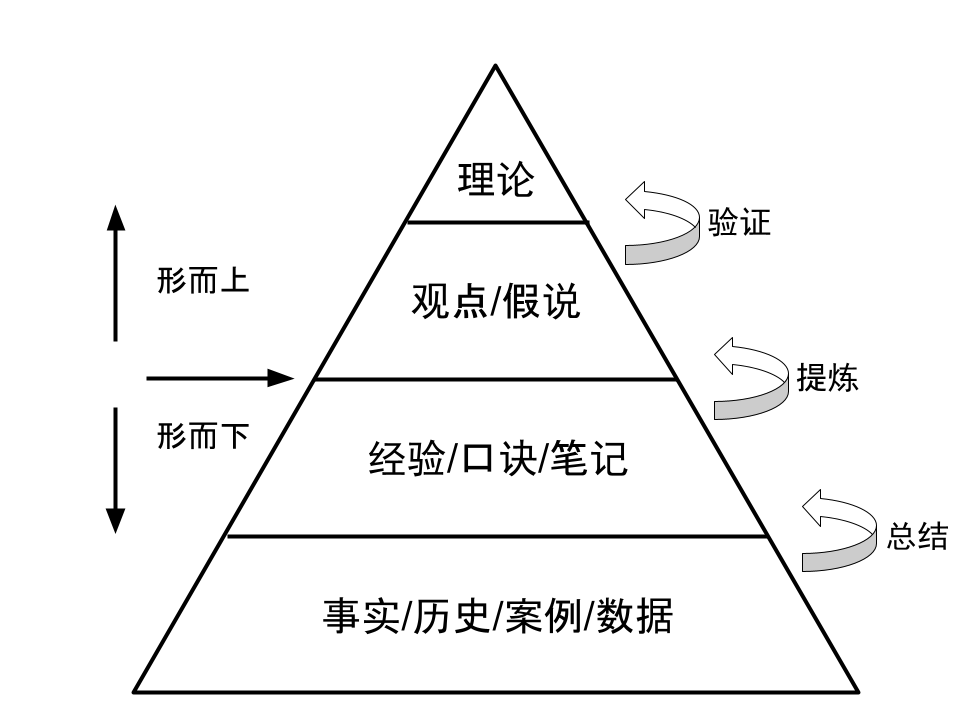
\includegraphics{data/knowledge} \caption[知识体系的构建]{知识体系的构建}\label{fig:unnamed-chunk-2}
\end{figure}

简单说就是你可以在知识层次超过背景组后就创建一个笔记系统来整合你的知识:形而下的基础数据与案例库、历史沿革及信息检索方法与形而上的理论观点库,区分强理论与弱理论并学会总结理论。要学会把新信息整合到这个知识体系中去并持续整合,形成完整独立的知识库,这样就不容易被新思想所迷惑,总能找到位置。如同世界观一样,你自己的知识体系也会被其他人的知识体系所冲击,此时要学习别人优点来丰富自己的知识边界而不是直接彻底否定与全盘接纳,后者常发生在宗教皈依过程之中。

\hypertarget{ux8ba4ux77e5ux504fux8bef}{%
\section{认知偏误}\label{ux8ba4ux77e5ux504fux8bef}}

真实世界中人会有一些很难避免的认知偏误。这些认知规律可能来自于动物本能或进化遗留的曾经帮助人类渡过难关的思维模式,也可能来源于有倾向性的判断失误,要认识并接纳这样的人性,很多行为是无法用理性解释的。

人的本能是认知偏误的重要来源。人会厌恶风险的,如果风险从1\%降到0\%会比从5\%降到2\%给人更大的安全感,人们会为绝对安全付出更大的代价。如果感觉安全或者有人托底,人们又会倾向于冒险,人们会认为放弃一件事的损失大于得到一件事的效益,即使损失与效益的绝对量是相同的。人们天生有保守化倾向,一旦感觉会犯错就会停止尝试,但不作为本身产生的危害可能更大。这一现象可以用来设计实验,例如用抽奖手段就会比处罚手段获得更高参与度。人们天生喜欢熟悉的东西或人,会从众,做比较时会喜欢用熟悉的概念或人群做参考而不是更大的陌生人群体。人也是短视的,会看重眼前的事而对长远的事经常顾不过来,例如学术报告能给人留下印象的往往是最后几张幻灯片或者说峰终效应,毕竟人们更容易记住那些让自己产生情绪波动的事。当你的受众是普通民众时,讲他们熟悉的例子要比画饼更能被理解,有时也许熟悉的例子并不能准确反映你的观点,但传播效果要好。为了减少认知负担,人们会倾向于脸谱化一些复杂事物,给这些东西一些抽象的设定或标签,然后对着这些设定或标签发泄情绪。人们喜欢形象化的东西,能画图就不要制表。即使内容不重要,简单重复性的刺激会加深其印象。人们天生搞不清楚概率与随机事件,经常把整体中发生某事的概率理解成个人重复做会发生某事的概率,把现象的概率看成预测性反馈性概率,虽然从回归意义上也有一定合理性,但基本属于一厢情愿。同时,大多数人搞不清观点与事实,例如科研结论通常是事实但经常被解读为一种观点,事实有真假无对错带有不确定性但观点经常带有倾向性与确定性,这对科学传播影响很大。

人具备思维惯性。人们会倾向于不计后果维护自己的一致性或之前的判断,哪怕自己已经知道错了,这种思维惯性跟科学思维是反的,科学思维倾向于质疑自己之前的判断。确认偏误也是思维惯性的一种,人们会倾向于主动确认那些自己熟悉或确认过的观点形成正反馈甚至形成光环效应,例如巴纳姆效应。人们会认为好的总会是完美的,甚至会把认可观点或人身上不相关的特性甚至缺点也识别为优点进行追捧。另外,每个人的经历不同或者背景知识不同,会对相同的事实产生不同的决策或判断,也就是说思维惯性对不同的人是不一样的。研究人员不能用自己的思维惯性去设计面向别人的实验,需要更多的同理心来兼容不同想法,写论文的时候也不能假设读者能顺着你思路想问题,毕竟有些人的思路非常跳跃。说白了人会脑补,读下下面这段文字,相信有英文基础的科研人员都知道是怎么回事,但问题是里面的单词大多数都是错的。我们的大脑会把错的识别为正确的,也会同样把正确的识别为错误,一定要警惕过于符合自己价值判断的理论与现象。

\begin{quote}
I cdnuolt blveiee taht I cluod aulaclty uesdnatnrd waht I was rdanieg. The phaonmneal pweor of the hmuan mnid, aoccdrnig to a rscheearch at Cmabrigde Uinervtisy, it dseno't mtaetr in waht oerdr the ltteres in a wrod are, the olny iproamtnt tihng is taht th e frsit and lsat ltteer be in the rghit pclae. The rset can be a taotl mses and you can sitll raed it whotuit a pboerlm. Tihs is bcuseae the huamn mnid deos not raed ervey lteter by istlef, but the wrod as a wlohe. Azanmig huh? yaeh and I awlyas tghuhot slpeling was ipmorantt!
\end{quote}

人会有逻辑自洽的倾向。这是人维持心态稳定的重要保障,人会倾向于解释一切的模糊因果理论但对概率模型及不确定性敬而远之,也会倾向于从噪声里找规律。好比一个律师打官司,他要做的就是收集事实证据形成证据链,但目的从一开始就定好了,那就是最大程度保护委托人。法庭因果看重的是叙事逻辑而不是真相本身,例如一个人随机杀人,那么其律师就要为这个行为构建行为逻辑,例如精神有问题或被别人指使。不论如何,法官或陪审团会从原因出发来量刑或定罪。然而,事实是这个人可能就是随机杀人,没有精神病史,也没有幕后黑手,但这个事实律师也好、法庭也好都会认为不可能,杀人不是意外,一定有历史或个人因素的原因,而这样的证据也可以很轻松从邻居或朋友评论中找到蛛丝马迹连成故事,可能是小时候踩死蚂蚁后笑了一下,可能是某次闲谈提到了武器,这些都是事实,但连成故事后可能杀人者都会突然发现,原来他逻辑上早就可能杀人了,甚至怀疑自己并不是随机杀人而是早有伏笔。人的记忆需要完整的逻辑连接来补充遗忘的部分,因此说的通的故事就会被认为是真实的。

但逻辑自洽经常跟事实对不上,好比一个科学家研究一个问题,他所能做的就是观察与实验,结论在观察中无法直接得出,要等数据符合统计要求了才能开展分析,经常连结论都没有而只是对之前一个观点的否定,要构建一组因果关系非常麻烦,需要反复多角度论证,如果论述不充分,科学家宁可保持未知状态也不会去任何一个数据支撑不充分的结论。这种因果观先看现象后形成论点,有时候还行不成很严谨的结论。例如病毒出现了,流病专家、基因组学专家还有分析专家都会在各自学科背景下对源头进行推测并报告不确定度,然而持法庭因果的人已经开始了审判。同样,法庭因果下人们只会采纳有利于自己的证据,但科研环境下不存在原告被告,需要同时列出实验阳性与阴性的结果,如果一组实验反复重复时只在小概率下阳性,那么这个现象不能被认为是真的。

认知偏误是所有人都有的问题,了解这些行为除了能帮助识别科研中存在的跟别人有关的问题,也能促进自我反省。通常而言,接受高等教育且从事科研的人经常会把自己的认知水平放到一个高位去跟别人交流,但事实上在犯错这件事上知识水平的预防效果非常有限。科研就是在错误中前进的,越快承认错误就能越快思考发现新的解决思路,当然也许新的思路还是错的。千万不要纠结结论的对错去评判别人,科研的重点在真假而不是对相对临时结论的价值判断。不要傲慢。

\hypertarget{view}{%
\chapter{科研现状概览}\label{view}}

了解科研现状要先了解现代社会及其形成过程,明白科研是现代社会的一部分,要优先解决现实存在的问题,也要学会从整体经济指标上观察现代社会结构并对科研这个行业进行定位。具体到当前,科研的基础研究生教育目前存在一些时代困境,读研会遇到扩招后的学历贬值、毕业延期问题,毕业后进行科研会遇到职业发展的爬金字塔过程及转行问题。而科研本身也遇到了可重复性危机等问题与趋势,下面就具体来讨论。

\hypertarget{ux73b0ux4ee3ux793eux4f1a}{%
\section{现代社会}\label{ux73b0ux4ee3ux793eux4f1a}}

现代科研隶属于现代政治经济系统,满足社会的需求是其存在的基础,至于是否满足个人兴趣爱好与远大理想,可认为是副产品。当然,这是从社会层面说,具体到个人千差万别。

\hypertarget{ux73b0ux4ee3ux793eux4f1aux7684ux5f62ux6210}{%
\subsection{现代社会的形成}\label{ux73b0ux4ee3ux793eux4f1aux7684ux5f62ux6210}}

首先,我们要了解现代社会运行的基本模式,其中陌生人分工协作是现代社会最突出的特色。社会,简单说就是一群人而不是一个人生存的行为与知识模式集合。

相比宗族或家庭为单位的原始聚居,古代与近代社会的发展不断突破着人们行为与知识范围的地理与血缘限制。在原始聚居条件下,人们终生活动范围有限,语言隔阂等也限制了信息交流,好的生存模式或经验很难传递到下一代或更远的地方,短暂的寿命基本都用在维持生存繁衍上了。当然,对原始部落的研究发现生活在其中的人并不比焦虑的现代人的快乐感受更少,但生活的自由度其实很有限(从另一方面讲,如果完全意识不到当今生活自由度可以改变其实也是一种内在幸福感,拥有更大自由度的人并不能完全体会到)。这种狩猎采集的原始聚居其实并不太需要共同的社会行为规则,但后来人们驯化了农作物与牲畜(其实很难讲谁驯化了谁,作物与牲畜也可能通过被驯化更好地传播了基因),进而从流动走向了定居。

定居后的社会出现了更细致的分工,例如一个村落需要祭祀、防卫、生产、医疗等部门维持生存结构,这种分工有着自己的生命力,一旦产生会让整体受益,同时也会让这种结构加强。同样的,这种分工模式并不惟一,但如果两个定居的社会共同体产生利益矛盾,最后剩下来的总是一种更有利群体生存的模式。这个模式下的行为规则形成了社会道德的起源。这同时也是一个路径依赖的过程,总会带有一些副产品例如民俗,很多时候我们就是通过副产品来回溯过去。如同对进化过程的研究一致,使用幸存者就是最好的或最合理的逻辑是不恰当的,我们需要通过回溯来发现一些制度历史上的合理性与偶然性,逻辑自洽并不代表历史真相,这点对科研认识也是很重要的。然而,这个阶段的社会政治经济体制依然很大程度被自然条件所控制,多数规则要么偏向农业社会,要么偏向商业经济。人类的视野逐渐开阔,但基于血缘与地域的多样化依然可以保留,直到更追求效率的技术与体制规则进一步交互作用,孕育出近代工业社会。

近代工业社会将分工与效率推向了极致,影响的范围从多个国家推广到了全球。伴随而来的就是一套基于陌生人交流法则的法制社会而不再依赖熟人社会里宗法或潜规则。交通技术例如航海、汽车、火车的进步打破了先进知识的区域内传播,所有国家都会倾向于遵循同样的工业标准,知识传播语言也尽可能一致例如使用阿拉伯数字计数或标准计量单位,法律也会去遵循共通的法则来处理陌生人间的关系。科学研究在这个过程中起了很重要的作用,而工业化也不断向科研提出需求,此时科学研究从精英们的兴趣爱好变成了巨大的财富来源,每一次技术革新都服务了社会,而几乎所有的社会经济体都会拿出资金支持科研。务实一点的国家或企业会对工程学优先发展,而对自然科学的支持则颇有情怀意味,毕竟一旦经济下滑,最先拿不到钱的都是基础科研等见效慢的学科。这种社会整体的功利主义自产生之时就展示了巨大的生命力,甚至不断影响了社会中个体的决策行为。

现代社会基本是延续了近代工业社会对分工与效率的追求且交流限制进一步被信息技术打破。现代社会的进步往往是构建在前人开拓领域之上的而不是像近代社会那样开拓全新的领域,特别在技术领域,新技术往往是很多现有技术的叠加或组合。对分工的追求导致工业品的生产与消费不再由一个人完成,人越来越嵌入到社会机器运转的齿轮之中,不用关心所需之物如何产生而更多关注其功用,而很多技术的使用者并不清楚原理,此时技术黑箱与魔法差异不大。而新产生的职业带有明显的目的性,例如心理咨询师就是要解决心理问题、营养师就是要给出最好的营养搭配、财务顾问就是能给个稳定的投资回报率、经济学家就是要能预警经济危机、科学家就是要能把核聚变搞成可控的等。不过,很多新产生的职业虽然事实上发展出了自己的术语或黑话体系,但并不能真的解决问题而仅仅是用专业感给现代人确定性与安全感,毕竟作为个体的现代人遇到自己知识外的问题除了寻求专家并信任专家外似乎也没有了探索其他知识领域的勇气。

这种分工导致的个体角色工具化或目的化经常给现代人带来困惑,现代人会很难理解科学结论里的概率而很快把概率转化为有用或没用这样的定性判断,例如传染病出现后现代分工制度会很快给出疫苗,但如果打了疫苗依然被感染就会被舆论放大,只是事实上疫苗的有效率从来都到不了100\%,现代人的世界观是决定论的而科学需要概率化的世界观。现代人会认为总存在专业人士来解决发生的问题,但事实上很多现在发生的问题历史上虽有类似,但需要因地制宜解决。我们的现代教育系统并不能及时提供解决新问题的人才而更多是传授有客观标准评判的知识,创新、灵感还有教材外自由发挥的内容很难培养与评价,但这些对解决问题很重要。

现代社会已经不存在真正意义上的通才了,甚至历史上的所谓通才知道的内容也不比现在完成义务教育的人多多少。唯一比较接近这个概念的是学者,不过学者现在如果不挂个专家头衔也很难发声。职业人士与专家看似一致但内核不同。职业人士追求的是标准化可持续的行业利益,专家则是从知识量来判断。职业化行业可以为了内部利益向大众营销价值观与品牌感,但专家更多是就事论事,远离利益讨论。很多现代人尽力维护的专家形象其实是为了维护自己的职业化饭碗别被时代甩开,但目光长远的专家学者则时刻准备迎接新时代。

分工对人的异化或者工具化既促进了现代社会经济发展效率,也制造了大量的现代社会特有的问题。现代社会对效率的追求主要是为了迎合工业革命以来的增长现象。现代社会犹如一台机器,能源供应以化石燃料为主,在几百年的时间里把植物上亿年从大气中固定的碳重新释放回大气。伴随技术进步,能源的供应似乎是有其他解决方案的,例如可再生能源与核能。在解决动力问题后,机器生产出的产品还需要被消费掉,支持消费需求的则同样是过去几百年,甚至更具体说就是二战以来才出现的人口大爆炸,近似指数增长的人口带来了巨大的需求与创造新需求的空间。不过,目前几乎可以确定伴随经济发展,全球人口增长的趋势将在几十年内终结,很多发达国家如果排除掉来自生育率较高的发展中国家新移民,人口事实上也早就停止增长了。或许现代社会会不断给现代人新的需求增长点,但人数只要不涨了,人口总需求端疲软的现象是一定会发生的,这会直接终结掉现代社会的增长逻辑。不过全局性衰退可能并不影响局部繁荣,当前人口虽然下降但依然向大都市圈集中,局部增长的代价是更大范围的衰退。

追求增长的发展逻辑其实自发破坏掉了很多农业社会以来形成的宗教世界观。现代人的伦理道德大都起源于农业社会甚至更早的狩猎采集社会,很多世界观跟增长是内在矛盾的,例如前现代社会的民俗宗教喜欢用轮回的概念,但轮回是需要收支平衡的,在信息交流效率低下的时代你可以说轮回到别处了也没法考证,但现在世界人口就摆那里了,农业出现前世界人口1500万左右,农业社会出现后到第一次工业革命中的1804年,世界人口才到达10亿。之后的两百多年里,这个数字变成了70亿。但并不是说1900年到40亿,事实上这个时间是1974年,甚至到达30亿都是1959年的事。这个快速增长时期的人口需要的前世从哪里来?清末四亿人口死了都别转去凑中国现在人口都得累积上几代人,阎王爷必须要掌握未来几百上千的人口变化才能在此时此刻凑够轮回总数,孟婆汤也得增加防腐剂来应对每天人数的波动。也许有人又要搬出六道轮回的理论补丁让人畜互相转生来凑数,但现代社会的绿色革命又不只是推动人口增长,畜牧业增长更是惊人,更不用说我们的生物制药行业为了提取某些不方面化学合成的物质而使用的工业级培养皿。物种虽然在经历大灭绝但数量上可一直都在增长,毕竟自从人掌握固氮技术以来人工固氮总量上已经超过了自然固氮,而有机氮是氨基酸的必要组成部分,因此现代社会里我们事实上``生产''出了自己形成了人口大爆炸。说白了轮回机制的提出者囿于时代根本预见不到一个增长主导的现代社会,后面无论怎么打补丁也会被统计事实打脸。

\begin{Shaded}
\begin{Highlighting}[]
\FunctionTok{library}\NormalTok{(showtext)}
\end{Highlighting}
\end{Shaded}

\begin{verbatim}
## Loading required package: sysfonts
\end{verbatim}

\begin{verbatim}
## Loading required package: showtextdb
\end{verbatim}

\begin{Shaded}
\begin{Highlighting}[]
\NormalTok{showtext}\SpecialCharTok{::}\FunctionTok{showtext\_auto}\NormalTok{()}
\CommentTok{\# 数据来自维基百科}
\NormalTok{wp }\OtherTok{\textless{}{-}} \FunctionTok{read.csv}\NormalTok{(}\StringTok{\textquotesingle{}data/wp.csv\textquotesingle{}}\NormalTok{, }\AttributeTok{check.names =}\NormalTok{ F)}
\FunctionTok{plot}\NormalTok{(wp}\SpecialCharTok{$}\NormalTok{population}\SpecialCharTok{\textasciitilde{}}\NormalTok{wp}\SpecialCharTok{$}\NormalTok{year,}\AttributeTok{pch =} \DecValTok{19}\NormalTok{,}\AttributeTok{xlab =} \StringTok{\textquotesingle{}年份\textquotesingle{}}\NormalTok{,}\AttributeTok{ylab =} \StringTok{\textquotesingle{}万人\textquotesingle{}}\NormalTok{)}
\end{Highlighting}
\end{Shaded}

\begin{figure}
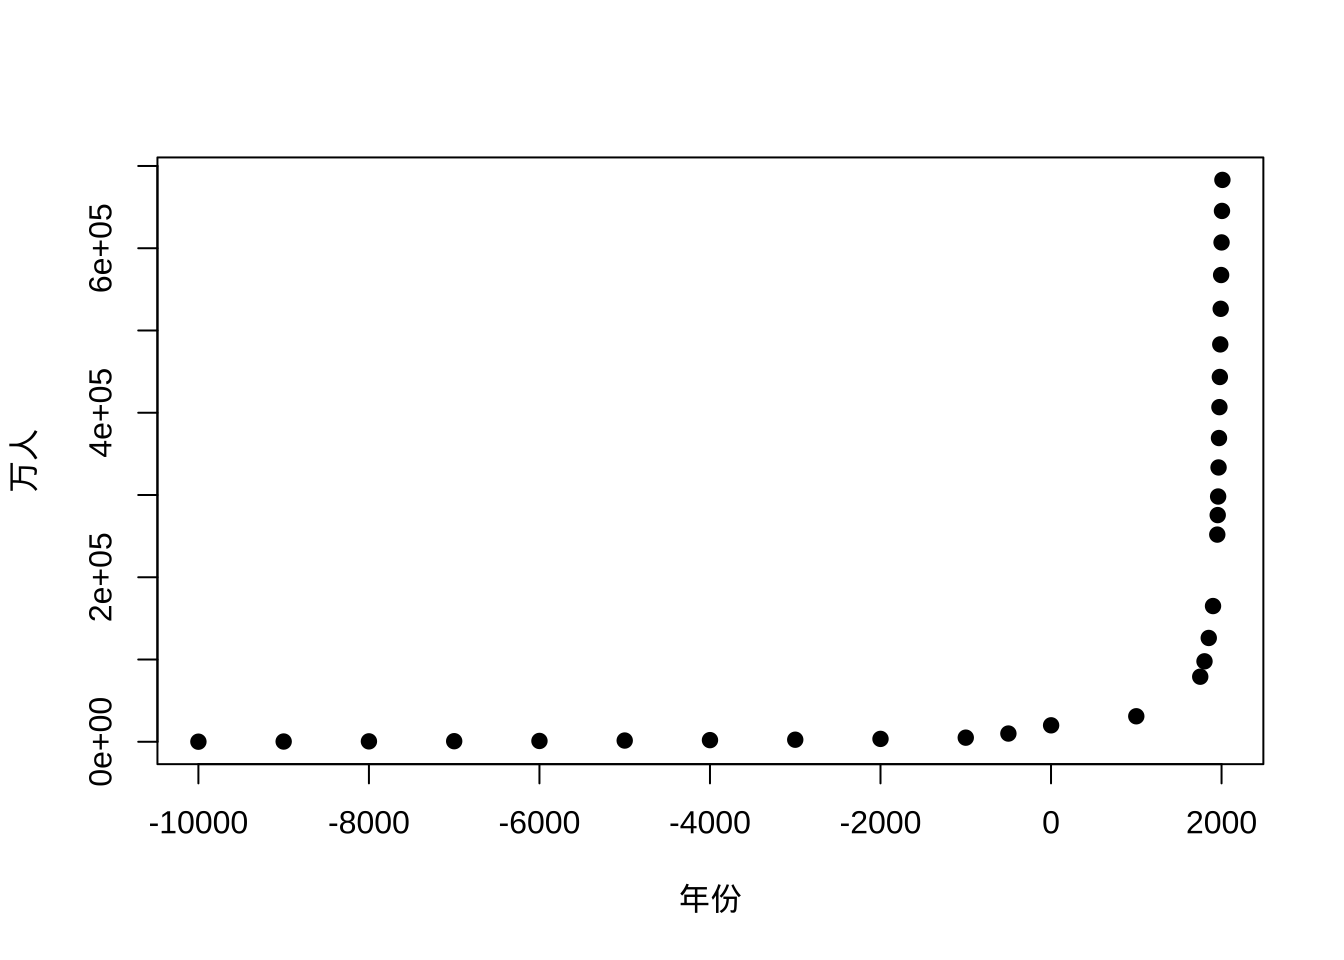
\includegraphics{sciguide_files/figure-latex/unnamed-chunk-3-1} \caption[世界人口变化]{世界人口变化}\label{fig:unnamed-chunk-3}
\end{figure}

此外,为了解决对未知而恐惧而构建的算命系统也经不起现代社会的检验,毕竟八字算命一共就能容纳561600种人,当今世界人口70亿,平均来看,每个八字有一万多人,也就是说八字其实不够用了,重复率太高,天煞孤星都不孤独,当然这类理论也有些打补丁的理论但明显是后来人意识到问题了增加的解释。现在保留下来的宗教都有一定世俗化趋势,模糊规避掉这些脱离实际的东西。现代社会的新宗教表现形式则更多是品牌崇拜、时间旅行、外星人这一类起码不会直接被经验事实证伪的行为与理念,否则根本经不起推敲。现代社会的增长逻辑是一种进步,起码对旧时代的破坏是很彻底的。

今天,增长逻辑还深深植入到现代社会的经济运转之中了,金融行业发展推动了资本的全球流动。资本所到之处会在区域内投资建厂、提供工作岗位、提升基础设施并创造繁荣景象,但同时当资本发现无法获益时就会毫不犹豫流向下一个价值洼地。这个过程之前会被限制在国家之内推动全行业进步,但全球化信息化的现代社会之中,资本流动更多考虑的是低成本高收益,因此我们会看到很多国家特别是小国家的行业门类是不全的。他们嵌在全球供应链上去发展,而具体品类产品的生产总是会集中到利润最高的几个区域或国家里且通过不断扩大规模降低边际成本,这同样是资本驱动,经济学上叫做比较优势。资本永远是逐利的,但当全球所有行业或区域因为各种限制或风险无法产生足够的利润,资本将会自行退出历史舞台。不过,现代社会目前还没有提出一个增长逻辑之外的经济运行方式与科技发展模型,以美元为中心的世界货币价值流通体系目前也遭受了很多新技术与保守主义的冲击,现代社会需要给出解决方案。更深远的影响则是个体对增长逻辑的信仰,现代人普遍展示出了对新技术与美好未来的向往且过去几十年这个现象也是符合增长信仰的,但从科学视角看增长更多是一种现象而非规律,会因为时代背景的不同而出现变化。

现代社会中维持文化多样性与个体-社会相互关系的思考不断涌现,它塑造了个体认知,个体认知却反过来反思现代社会的诸多问题例如极端民族主义、保守主义还有宗教的崛起、环境保护、气候变化、社会隔离与歧视、机会公平、贫富差距、人口老龄化、战争暴力、谣言传播、经济危机、金融危机、人工智能等。这些问题的根源有相当比例是社会政治经济体制的构建过程出现了漏洞,而今的科技发展把一些问题放大了,或者说这个系统需要打补丁了。虽然在意识形态或经济发展模式上现代社会有些概念上的区分,但说到底都是去构建或选择一个让大多数人能接受的体制,然后能够去解决发展中出现的问题。如果问题足够严重,所有现代国家会搁置争议联合起来解决,毕竟本质上现代社会制度都是解决发展问题的。而发展中问题的出现自有其内在规律,不会主动迎合现有社会体制。

\hypertarget{ux73b0ux4ee3ux793eux4f1aux7684ux7ed3ux6784}{%
\subsection{现代社会的结构}\label{ux73b0ux4ee3ux793eux4f1aux7684ux7ed3ux6784}}

当前社会运行方式也可通过基本经济指标这个角度来进行整体解读。2020年中国人均国内生产总值达到了一万美元,也就是一年全国创造价值总和大概14万亿美元。全国有约不到8亿就业人口,另外有6亿多或老或小目前没法创造劳动价值,学龄前跟上学的、家庭主妇/夫还有吃退休金的老年人与无劳动能力的群体事实上还是靠家庭与政府补贴养的。在发达国家美国,也有大约超过一半的人口是不领工资不就业的(这个数据川普竞选总统时曾经用过,吃准了普通人算不清楚就业人口与总人口的差异,失业率其实只算满足就业条件人口与实际就业人口),毕竟美国年龄结构比中国更老龄化一些。同时,伴随老龄化与少子化,中国就业人口规模事实上在2017年已经见顶,未来就业人口比例会更低。

\begin{Shaded}
\begin{Highlighting}[]
\CommentTok{\# 数据来自世界银行}
\NormalTok{e2p }\OtherTok{\textless{}{-}} \FunctionTok{read.csv}\NormalTok{(}\StringTok{\textquotesingle{}data/e2p.csv\textquotesingle{}}\NormalTok{, }\AttributeTok{check.names =}\NormalTok{ F)}
\FunctionTok{plot}\NormalTok{(e2p}\SpecialCharTok{$}\NormalTok{World}\SpecialCharTok{\textasciitilde{}}\NormalTok{e2p}\SpecialCharTok{$}\StringTok{\textasciigrave{}}\AttributeTok{Country Name}\StringTok{\textasciigrave{}}\NormalTok{,}\AttributeTok{pch =} \DecValTok{19}\NormalTok{,}\AttributeTok{xlab =} \StringTok{\textquotesingle{}年份\textquotesingle{}}\NormalTok{,}\AttributeTok{ylab =} \StringTok{\textquotesingle{}世界就业人口比(\%)\textquotesingle{}}\NormalTok{)}
\end{Highlighting}
\end{Shaded}

\begin{figure}
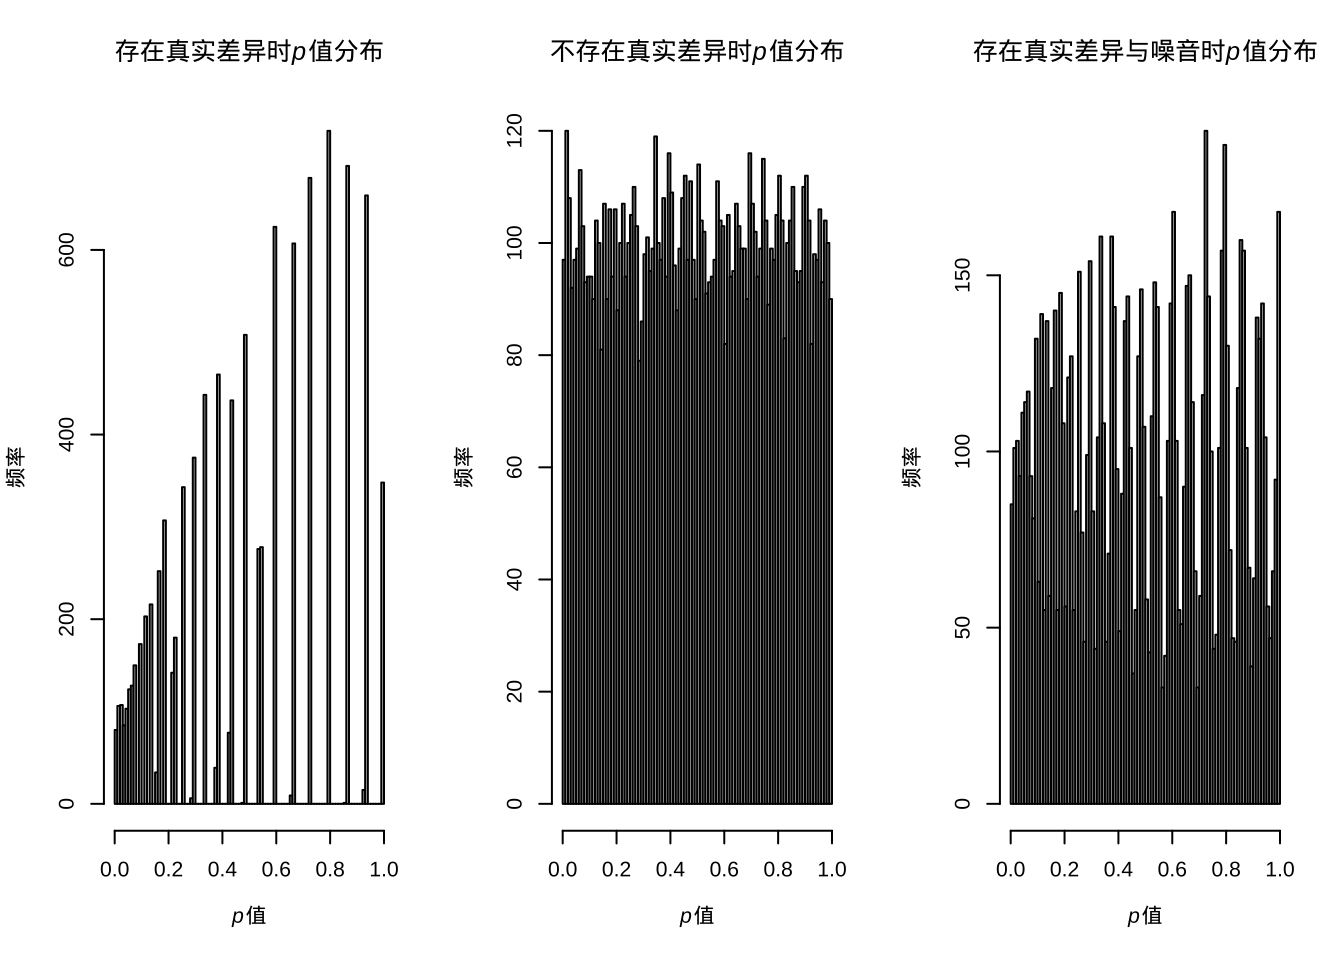
\includegraphics{sciguide_files/figure-latex/unnamed-chunk-4-1} \caption[世界就业人口比的下滑趋势]{世界就业人口比的下滑趋势}\label{fig:unnamed-chunk-4}
\end{figure}

另外,人均国内生产总值一万美金跟人均收入一万美金也是两个概念,企业的支出成本比绝大多数人拿到手的薪资要多,要考虑物料磨损、税费等开支。虽然这个比例不太固定,但一般认为大概五到六成是人均收入,美国2019年人均国内生产总值大概6.5万美元而家庭人均收入则成了3.3万美元,中国人均年收入也就大概5000美元,这个人均的基数是总人口而不是就业人口,把儿童老人也给算进去了。因为就业人口恰好也是总人口的五六成,所以人均GDP其实歪打正着跟就业人均工资其实差不多。

在接近八亿就业人口中,其中四成是农业人口,中国目前的城市化其实也就搞了五六成,城乡收入差距大概三比一。因为存在收入差距,以后农业人口还得萎缩,会有越来越多的乡村消失流向收入较高的城市。中国就业人口从事的行业超过百万人规模的大概有三四百个,差不多对应上了所谓三百六十行,大头在制造业、建筑与教育。按产业划分农业解决了其中大概两亿,制造业也是大概两亿,第三产业解决了剩下的不到四亿人。所谓中国制造其实是约两亿就业人口在支撑的,且这个数也在逐年萎缩。同时,每年城镇新增就业人口大概一千多万,同时也有接近千万的人退休,这些就业数据如果有概念了后面的很多趋势推算就比较简单。互联网上活跃的人大多是学生跟有工资没成家的职场新人,对养家糊口缺少感知。事实上,支持经济的中青壮年其实在现代社会中起着创造经济价值且补贴其他年龄段的作用,如果就业人口低于五成这个现代国家的经济游戏就会玩不下去。科研对于现代社会需要解决的一个现实问题就是在人口不能支持经济可持续运转时用新技术来降低社会运作的成本。

现在我们看下城市数据,全国有两三百个地级市,县级单位有接近三千个,城市实体(不论县级还是地级)除了一线城市外,人口基本在几十万到几百万之间。对于地方经济,如果某一个行业解决了过万的就业岗位,其对地方政府财政收入的影响就大概率超过百分之五,显著影响地方经济发展与社会稳定。例如,任一地方政府的公务员与事业单位就业人数都可看作一个大行业,地方上单一企业就业人数如果过万,年产值基本都是大概不低于十亿人民币的规模,按中国的企业税,地方政府拿上亿不成问题,多的时候能解决地方公务员四五成的工资。说这些是想说明对于地方政府,几千上万的就业看起来少,实际特别诱人,同理在美国经常看到地方议会为了几千就业岗位吵得昏天黑地,实际原因就是背后都是真金白银利益相关。

此外我们看一下行业规模,年产值过万亿美元的细分行业是不存在的,因为全中国一年就14万亿美元的总盘子去让几百个行业大类去分,但确实有行业产业能过万亿人民币,说白了就是医药、地产与金融,但这些行业都有从业门槛,要么是资质、要么是资金、要么是专业术语体系,一般人不好进去,因此从业者也就能享受超过平均数的收入,不过从业人数规模也都是百万级的了。如果进一步细分就比较有意思了:

对于一个千亿规模市场,按照行业平均薪酬其从业规模大概在百万,如果其服务目标用户是几亿,那么每年要从用户手里拿几百块钱才玩的下去,教育、医疗、通信、水电、公路、铁路、家电公司、母婴基本就是这类行业。通常千亿规模市场的用户都是上亿的,几千万都不太可能,这意味着一年收几千万用户上千块钱,就我国居民消费能力而言,也就餐饮行业能勉强达到用户规模与开支。几百万用户就更不可能了,用户一年掏上万块钱意味着居民年收入三成,不过房地产有可能达到这个规模。只要你了解你自己的开支,差不多就能估计这类温饱行业规模。因为关系国计民生,这些行业国有化程度比较高或被国家监管,资本回报率低但稳定。一个城市里几乎所有人都会成为用户。

对于一个几百亿规模市场,按照行业平均薪酬其从业规模大概在几十万,这个规模就能解决些温饱外的需求了,几千万用户年消费几百或上亿用户年消费几十的行业非常多样了,服装、高端家电、图书、电影等比较小康的行业是在这个量级的,这个量级市场上因为用户群可以进一步缩小到百万,单人支出过千其实也可以支撑很多广义上的兴趣了,例如手游、直播、旅游、健身等基数不那么低的中高开支爱好,这个量级的市场特别受资本关注,但眼下基本伴随移动互联网普及而饱和,会有新增长点,但整体规模应该是稳定了。一个城市里大概十分之一的人会成为用户。

几十亿规模的行业就是小众爱好行业,单一行业从业人数不过几万人,用户在几百万到上千万的规模,年开支很少低于几百的,大都超过千元。前些年比较红的球鞋、邮币还有海淘基本就是这类规模市场的代表。从人群基数看,单一城市只有百分之一甚至更少的人是这个市场的目标客户,也就是几万人,这个用户群在前互联网时代基本形不成气候,现在有了网络同一地方的小众爱好者可以在网上形成团体交流并产生持续购买力,这种规模的市场网络上是有可能找到个日活过几千的相关论坛。应该说这个规模行业特别容易受到控制、形成垄断或意见领袖,因此盈利空间会很大。用户基数越少,年开支约高,闷声发财的概率就越大。目前资本开始关注这个量级市场,虽然总盘子不算大,但回报率可以做到很不错。

到了几亿规模的行业基本就是诈骗重灾区了。因为全国目标用户在几万或十几万人,单人年消费就一定要高,几千上万比较常见。也有正规的行业,不过肯定非常小众了,例如汉服、地方土特产之类的。单一城市只有千分之一甚至更少的人是这个市场的目标客户,也就是几百上千人,这类行业就不需要市场调研了,直接针对客户坑就完了。资本是不可能投几亿规模的市场的,你投个几千万就算市场全拿下来了也就是十倍回报率,配合较高风险几乎就是有去无回。这种规模市场从业人数全国也就几万人,要么集中到一两家企业,要么就是各地游击战。

行业规模的下限就是几亿,再往下资本肯定不会介入,诈骗犯都嫌弃目标客户少且客单价低。毕竟不论哪个职业,在现代社会你要一年开不出人均GDP以上的工资,根本就不会有人去冒这个风险,合法搬砖也比违法赚钱香。不过作为小众爱好,几千万的行业规模也还是有的,撑不起全职可以是业余兼职做,有的则会抬高客单价来定向找高净值人群。估计这些是说明一些自媒体拍脑袋渲染的所谓魔幻现实主义现象有些确实存在,但有些从行业规模估计上就不成立或无法可持续发展,后者更重要,所以有些故事当都市传说看看就够了,不要把世界想的太恐怖。

除了行业规模,我们也可以从消费品价格区间来了解现代社会,十分之一可以看做是区分现代工业品贵贱的标准。在一个平均收入一万美金的现代国家,一年花费超过一千美元的物品都可以算是昂贵的产品或者说奢侈品。奢侈品在不同国家的定义是不一样的,对不同收入人的定义也不一样,如果品牌目标是收入百万人群的话十万左右的东西是不掉价的。对普通人而言,日常开支中家电等的定价如果你转化为年均开支就会发现大概都在月收入百分之十这个量级,日常开支单品中耐用品的价格定在月薪百分之十而消耗品通常定价在日薪百分之十。绝大多数商品单品年均定价都不会超过普通人月薪,否则要么是诈骗载体,要么是只面向高收入人群的奢侈品,而且奢侈品定价过高也面临有价无市的情况。本质上商品的市场价格都是比目标人群平均收入略高一点的而不是根据成本定价,这样也能维持住一点增长逻辑下的良性通胀。想快速了解一个地方,考察行业规模通常不现实,但通过超市里当地食品定价可以大致推断人均收入水平,进而估计当地发展的发展水平,这也是现代社会才有的特征。

总的来说,对于一个现代社会中可持续行业,从业人员的人均收入要达到人均国内生产总值,客户群在全国尺度上要配合年人均消费额来估计行业规模,然后根据行业规模也可以估计其垄断程度与发展阶段。前面的估计换成美元,基本就是全世界的市场规模,虽然差个几倍有可能但应该不会出现数量级差异。一个爱好想成为一个正儿八经的职业,光有兴趣是不够的,得让这个时代的工业化水平与人口规模配合你。就一个人口过千万的现代国家而言,千分之一的人的小众爱好就可以形成过万的用户群,年消费过千,就会出现千万市场。就从业人员角度,全国总人数不过万,一般一个县级单位才有一两个人从业,那么就没有行业标准。兴趣爱好人数低于千人规模,用爱发电,形不成行业,淘汰或非遗保护。而社交平台小众垂直领域的意见领袖真实粉丝不会低于千人,至少万人才可能支持用爱发电,会有一定广告价值。理解现代社会分工的状况与规模,对于科研人员找社会定位很重要,在细分领域很重要的突破可能在更大行业里意义有限,不要把自己的研究看得太重要或太不重要,都是现代社会的一部分而已。

\hypertarget{ux73b0ux4ee3ux79d1ux7814ux7684ux5b9aux4f4d}{%
\subsection{现代科研的定位}\label{ux73b0ux4ee3ux79d1ux7814ux7684ux5b9aux4f4d}}

毋庸置疑,科研对于社会发展现实问题的解决是一个靠谱的选择,其他选择例如宗教、回归原始生活更多的是一种消极的保守策略,选择那些方法并不会真的解决问题。同时,现代社会的持续运转与科学求真求实的目标也是因为恰好科研会促进经济而看似一体,实际上要是魔法真能促进现代经济的发展,科学家估计还会是隔三差五就被送上宗教法庭的高危职业。现代社会运转看重的是价值判断与决策而非探索真理或进行事实描述,这是科学家这个身份天然需要调和的矛盾。

如果给科研在现代社会中立块大牌坊,最好的题词就是从方法论层面解决社会问题。换言之,科研总是面向问题解决问题的一个社会分工,是一个职业,既不神圣也不低俗,从事这个职业的人总在用科学方法论解决实际问题,或者揭示问题本身并为问题找一个解释。这个需求是根源,也就是说如果你科研自认为做的不错但跟现实脱节,那么即使留在象牙塔,也会面临自我认同与社会认同不协调的困境。一般来说,热点基础学科里悖论会比较多,热点应用学科则是看实际问题。科研对很多从业者而言是追求真理的一种实现手段,不过现代社会关心发展中的问题胜过关心真理本身,现代增长逻辑下有时看不了很远,所以需要研究人员开动脑筋将两者的目的在研究具体项目中统一。

作为一个产业,现代科研也需要讲投入产出,所谓投入主要是国家拨款或私人基金,而产出则是高素质的人才与解决实际问题的技术或方案。有产业就有竞争,科研行业也存在明显的资源集中状况,知名高校与研究机构为了争取资源会去竞争人才这一核心生产力。在高校研究所层面就是要争取在各类排行榜上有个好名次或跟同水平的学校绑定为联盟共享资源,这样就能持续吸引到好的生源产生正反馈。运行一个科研机构本质上与运行一家企业差距不大,行政职能部门也要遵守现代企业管理制度。唯一有区别的是教职系统,目前国内高校逐渐打破原有事业单位体制,采取长聘制度,对年轻人给予更多资源支持的同时也用终身教职的高考核标准来保证学校的持续性科研产出。事实上,由于科研行业本身知识更迭快,接收新知识相对快的年轻科研人员做出成果的概率是比资深科研人员要高的,但同时年轻科研人员缺乏科研资源整合管理经验,因此现代科研机构普遍会去竞争成果优异的年轻人或研究体系完整的成熟团队。不过,很多高校过分看重短期科研产出,用宽进严出方式招收长聘教授,这造成了所谓``养蛊''的现象。伴随国内博士毕业生越来越多,应该着力拓宽博士的就业途径尽快服务社会而不是留在学校里刷论文指标。同时,现代高校也特别看重校友资源,因为校友会为学校带来很多持续保持领先地位的资源。另外一个产出是科研论文,早期看数量后期看质量,一个简单的标准就是成果是否值得放到高等教育教材之中。

科学家是现代职业的一种,作为职业价值判断总是第一位的,不然没饭吃。打个比方,你申请了一笔经费研究污染物A对疾病甲的影响,做了半天发现没影响,你要是打算转行那卷铺盖走人就行了,但科研领域的经费逻辑是成功导致成功,你第一个项目不成功第二个申请就费事了,然后你就会看到很多人穷尽各种统计方法去找一个p小于0.05的结论来结题。要是真有科学思维会马上意识到这样的发现发表就是终点,后面的人会引用但懂行的肯定知道不是什么重要发现。行业职业化会导致从业人员价值观指导研究,好比戴着有色眼镜做科研,经常只能报道或者拼凑有影响的结果,这显然不是什么科学思维,但这种思维已经深入人心。

坦白说,现代职业科研体系并不需要每一个从业人员都有科学精神,对于一所现代化大学或研究机构,搞钱搞人才搞名声才是硬道理,科学精神反而属于负战斗力,经常把一些看起来很成功的项目给搞垮。科研明明是件需要试错的事,却被现代化管理搞成了需要不断成功才能持续下去的励志小故事。现在很多科研从业人员喜欢成功多过喜欢科研,他们越来越像项目经理与老板,产出的是流水作业的废纸,对他们而言科研只是体面工作与薪资的保证,而这也是现代化社会运转的一部分。有意思的是,因为当前推动社会进步的主要是技术组合而非科学,所以其实现代科研在某种程度上是鼓励论文流水作业与强者恒强不容置疑的模式的。不过,没有科学思维在这个行业很难走远并体会到乐趣。

现代科研很多时候要求产学研结合。但其实产业界与学术界遵照的是完全不同的评价标准,用产业要求来评价学术成果通常过于超前了,同时用学术要求来评价产业问题经常会搞出脱离实际的笑话。但现代社会发展到今天,很多发展很快的行业里最尖端的技术往往已经不在校园作坊里了,很多跨国科技公司在某些领域的研究水平已经超过了世界上大多数的研究机构。因此,一定要重视与企业的合作与互相学习借鉴与渗透,及时更新相关的课程、教材与案例库。否则,象牙塔培养出的人既不适应产业要求又用繁杂的学术名词维持自己的专业感,社会上很快就会形成学历无用论等反智趋势,会波及那些真正认真研究实际问题的同行。

同时,科研行业本身也需要跟其他现代社会行业竞争国家或社会能分配的资源,也是一个利益集团,需要民选代表到国会或人大去参与财政的分配。即使国家已经表态重视科研也要持续发声,因为反科研集团也是现代社会利益集团中的一部分,公众有选择娱乐至死生活方式的权利、资本有逐利的习惯、宗教也无时不刻准备争夺话语权。社会上的思潮起起伏伏,五四运动之后对科学精神的追求虽然深入人心但还远远不够,科研行业如果式微,现代社会会很快退回到农业社会。不过,科研行业内不同学科也要去抢所有的科研经费分配,充满了复杂的博弈过程,原来是陌生人之间,以后可能会发展到人跟机器或规则之间。

放到个人视角下,这个职业也是有温饱小康问题的,这个职业有光环,但退却光环都是一个个为生计奔波劳碌的现代人。当然,不同人有着不同的生计标准,现代人想扩大影响力需要给自己打上高识别度标签,但为了找回自己又要去摆脱标签的束缚,这种反覆让事业发展与个人需求经常脱节。目前科研人员的社会待遇基本靠国家政策,资本会青睐科技行业但更多需要工程师而不是科学家,不过相信科研人员的整体待遇与分配法则会改善。

\hypertarget{ux7814ux7a76ux751fux6559ux80b2}{%
\section{研究生教育}\label{ux7814ux7a76ux751fux6559ux80b2}}

研究生虽然在学术圈里地位最低但却是现代科研的主力军,因为社会对高学历人才的需求、高校对就业率的追求及社会中普遍存在的``深造''思维,在读研究生群体这两年在快速壮大,甚至超过了1999年大学扩招前本专科生群体总人数,而很多研究项目事实上是劳动密集型产业而培养欠缺。这就造成了研究生教育的学历贬值、毕业延期、学术职业发展越来越难及解决问题综合性能力不足的问题。

\hypertarget{ux7814ux7a76ux751fux84c4ux6c34ux6c60}{%
\subsection{研究生蓄水池}\label{ux7814ux7a76ux751fux84c4ux6c34ux6c60}}

2020 年国内研究生入学考试报名人数刷了新高,达到 341 万,而这里面应届生与往届生人数相当,报录比在扩招的大背景下还在不断降低。有一个很有意思的现象,报考研究生的人数并不是一直上升的,事实上,2007 年、2013 年都出现过报考高峰然后下一年回落的情况,回落可能跟当时经济形势上行有关,当社会岗位需求旺盛时,两三年的学位投资就可能是一笔很高的机会成本。但 2016 年起,研究生入学考试报名人数重新上升,这侧面体现了毕业生对就业的担忧。而且往届生与应届生报录人数同时增长,说明毕业生普遍认为学位比工作更有价值,或者说本科就业形势不佳。

\begin{Shaded}
\begin{Highlighting}[]
\CommentTok{\# 数据来自中国考研网 http://www.chinakaoyan.com/info/article/id/77817.shtml}
\NormalTok{gradapply }\OtherTok{\textless{}{-}} \FunctionTok{read.csv}\NormalTok{(}\StringTok{\textquotesingle{}data/gradapply.csv\textquotesingle{}}\NormalTok{)}
\FunctionTok{plot}\NormalTok{(gradapply}\SpecialCharTok{$}\NormalTok{application}\SpecialCharTok{\textasciitilde{}}\NormalTok{gradapply}\SpecialCharTok{$}\NormalTok{year,}\AttributeTok{pch =} \DecValTok{19}\NormalTok{,}\AttributeTok{xlab =} \StringTok{\textquotesingle{}年份\textquotesingle{}}\NormalTok{,}\AttributeTok{ylab =} \StringTok{\textquotesingle{}研究生报名人数(万人)\textquotesingle{}}\NormalTok{)}
\end{Highlighting}
\end{Shaded}

\begin{figure}
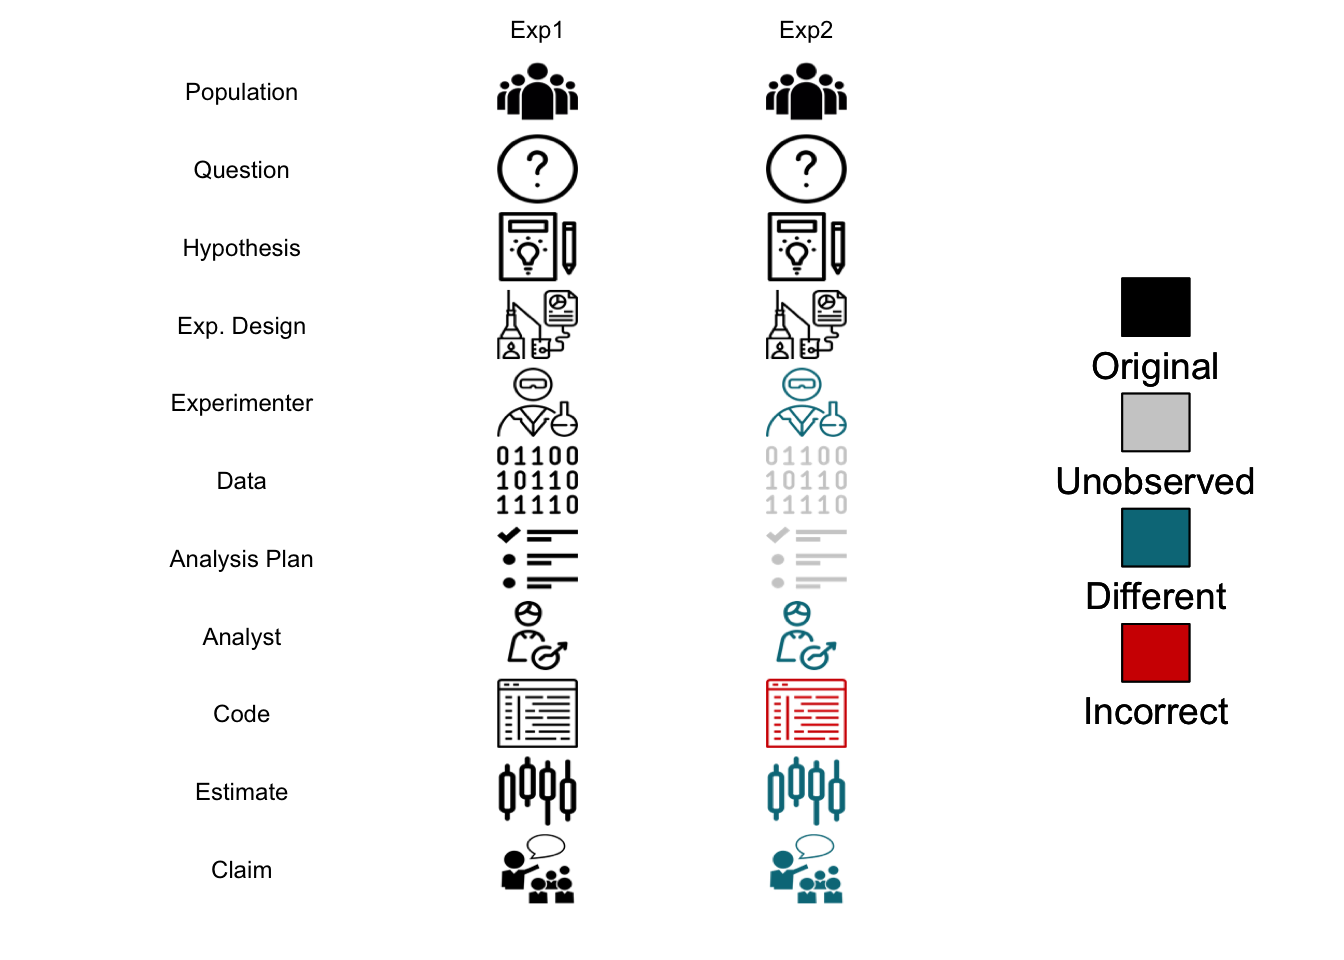
\includegraphics{sciguide_files/figure-latex/unnamed-chunk-5-1} \caption[中国研究生报名人数变化]{中国研究生报名人数变化}\label{fig:unnamed-chunk-5}
\end{figure}

我们再看看高考,中国高考报名人数在 07-09 这三年都突破了千万,此后人数有所,但最近几年又突破千万。不过高考录取人数则持续上升,因此如果就业形势不变,报考研究生的人群基数也会增长。

\begin{Shaded}
\begin{Highlighting}[]
\CommentTok{\# 高考报名与录取数据来自教育部网站}
\NormalTok{cee }\OtherTok{\textless{}{-}} \FunctionTok{read.csv}\NormalTok{(}\StringTok{\textquotesingle{}data/cee.csv\textquotesingle{}}\NormalTok{)}
\FunctionTok{plot}\NormalTok{(cee}\SpecialCharTok{$}\NormalTok{application}\SpecialCharTok{\textasciitilde{}}\NormalTok{cee}\SpecialCharTok{$}\NormalTok{year,}\AttributeTok{pch =} \DecValTok{19}\NormalTok{,}\AttributeTok{xlab =} \StringTok{\textquotesingle{}年份\textquotesingle{}}\NormalTok{,}\AttributeTok{ylab =} \StringTok{\textquotesingle{}人数(万人)\textquotesingle{}}\NormalTok{,}\AttributeTok{ylim =} \FunctionTok{c}\NormalTok{(}\DecValTok{0}\NormalTok{,}\DecValTok{1100}\NormalTok{))}
\FunctionTok{points}\NormalTok{(cee}\SpecialCharTok{$}\NormalTok{entrants}\SpecialCharTok{\textasciitilde{}}\NormalTok{cee}\SpecialCharTok{$}\NormalTok{year,}\AttributeTok{col=}\StringTok{\textquotesingle{}red\textquotesingle{}}\NormalTok{,}\AttributeTok{pch =} \DecValTok{15}\NormalTok{)}
\FunctionTok{legend}\NormalTok{(}\StringTok{\textquotesingle{}bottomright\textquotesingle{}}\NormalTok{,}\AttributeTok{legend =} \FunctionTok{c}\NormalTok{(}\StringTok{\textquotesingle{}报名人数\textquotesingle{}}\NormalTok{,}\StringTok{\textquotesingle{}录取人数\textquotesingle{}}\NormalTok{),}\AttributeTok{pch=}\FunctionTok{c}\NormalTok{(}\DecValTok{19}\NormalTok{,}\DecValTok{15}\NormalTok{),}\AttributeTok{col=}\FunctionTok{c}\NormalTok{(}\StringTok{\textquotesingle{}black\textquotesingle{}}\NormalTok{,}\StringTok{\textquotesingle{}red\textquotesingle{}}\NormalTok{))}
\end{Highlighting}
\end{Shaded}

\begin{figure}
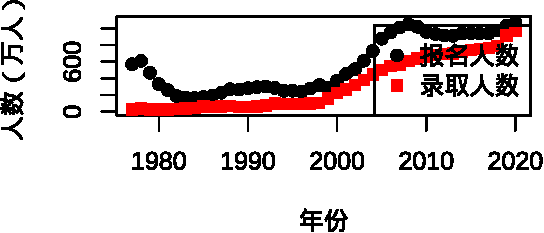
\includegraphics{sciguide_files/figure-latex/unnamed-chunk-6-1} \caption[中国高考报名与录取人数变化]{中国高考报名与录取人数变化}\label{fig:unnamed-chunk-6}
\end{figure}

可以预计如果研究生持续扩招,搞考研培训、出国培训、期刊校稿还有高校教职将出现最后的快速发展窗口,之后将进入稳定或衰退期。然而,这之前我们体会更明显的则会是更多关于研究生团体的讨论与新闻调查,我们的研究生教育发展可能还跟不上研究生团体扩大的速度,中间的差距是一头典型灰犀牛,潜伏巨大系统性危机。

从学生角度看,眼下的研究生报考热潮跟经济压力有关而跟科研兴趣没啥关系,所以很有可能出现学生自认打工仔的情况而在混日子等就业的情况,高校或研究所的心理辅导如果跟不上会出不少极端问题。从导师角度看,近二十年的高校扩张吸收了大量新导师,而持续增加的劳动力所需要的管理经验基本都比较欠缺,毕竟他们读研时周围没那么多学生,研究生无指导或指导过激情况会不断出现。我们会在近几年看到一系列因为研究生极端事件而采取的改进,但能否做到预防,就看高校研究所的领导团队是否有意识了。

其实当前已经有一个解决方案了,那就是专业硕士。专业硕士直接对口就业,很多专业硕士的学位的业界认可度也比较高,例如工商管理硕士、法律硕士等。因为其对应的学术硕士的就业需求不算明确而很多选择读研的学生目的就是就业,相信未来专业硕士的招收比例会不断上升来迎合这个趋势。不过,确实有些学科无专业硕士的就业认可度而仅仅是想通过扩招来的名额吸纳廉价劳动力,这样不但会造成学术硕士对专业硕士某种程度上的歧视,对学生而言也无法解决其最关心的就业问题。专业硕士的培养要比学术硕士更贴合实际需求,对应用的要求更高但可以适当放松学术创新能力,不过现在很多导师并不能给予合适的指导,这方面也需要时间来磨合。

研究生身份更像是一个容器,容器里面的是 22-30 岁的年轻人,都有着明确的导师学生关系,这个容器越大,微弱的声音就更可能汇聚成大的声响。这个群体的心理健康连同与之紧密相关的导师的心理健康都非常重要,这里面研究生群体是弱势群体,很多研究生对情绪调整可以说毫无头绪,这是成长的烦恼,但高校的象牙塔属性与导师制并不保证健康成长。社会里公司可以靠成熟持久的制度职场教做人,导师学生关系却永远只会是二到八年的临时身份,显然后者出问题概率更高。导师靠自觉来解决问题也并不容易,可以借鉴的经验基本就是个人成长经历,这玩意多半是个邻居孩子的故事,励志还行,并不能捕捉体会到当下研究生的真实感受。资源、机会、奖惩、社会整体就业压力都面临公平效率间的平衡管理,偏巧这玩意在日益侧重研究的高校研究所里是不教的。师生交流不畅会成为今后研究生教育问题重要来源。

读研的虽然是人口少数,但这部分人口掌握了相当的网络话语权。显而易见,未来几年我们社会里最有时间在网上发言的大学生研究生群体会持续走高,我们应该会看到更多对这个群体的讨论与新闻。事实上,千禧一代在制造话题上从来都是行家,他们伴随互联网技术崛起而成长,他们普遍教育程度的走高对整个社会,特别是舆论引导会产生巨大影响。如果你去回顾下这些年社会新闻的焦点,基本都能找到千禧一代的身影。他们在中国人口基数中比例很高,裹挟了上一个婴儿潮作为父母,可以说对很多经济形态例如网红经济、知识付费、新零售、消费升级、租房市场等提供了消费需求。他们的消费与网络话语权决定了新兴市场会听取他们的态度而不是大多数人的态度,而新闻媒体从来都是求新的。现代社会本质上就是知识精英的社会,因为现代社会的大厦只能通过各类专门知识来管理,单纯资本或人口不解决问题。

这是一个浪潮,浪潮的下一端是人口结构的变化,千禧一代可能是世界范围内最后的婴儿潮。眼下发生在非洲东南亚的那一拨可能有人口红利,但没有互联网同步发展的技术红利,如果不出现类似互联网的普惠技术,很多发展中国家事实上或者说政治上不存在多大的发展空间。所有问题都可能是时代问题,这几年有,下几年就没了,但身处时代之中的人往往是最容易看不到问题的。

\hypertarget{ux6bd5ux4e1aux5ef6ux671fux95eeux9898}{%
\subsection{毕业延期问题}\label{ux6bd5ux4e1aux5ef6ux671fux95eeux9898}}

根据教育部的公开数据,近20年研究所与高校的研究生录取比例均大概为1:3,硕士和博士都在扩招,但对硕士的扩招力度远高于博士。20年前我国每年一共招收6万多研究生,现在仅博士每年就录取10万多人,硕士则扩张了10倍有余,录取人数达到每年接近一百万,研究生在校生规模也在快速增长。从研究生毕业状况看,伴随扩招,每年的招生人数与毕业人数有相当的差距。但比较奇怪的是,博士招生人数在不断增长但毕业人数的增长幅度却增长有限且长期少于前几年的录取人数了,这基本暗示延期,特别是博士延期的常态化。

\begin{Shaded}
\begin{Highlighting}[]
\CommentTok{\# 数据来自教育部}
\NormalTok{graduate }\OtherTok{\textless{}{-}} \FunctionTok{read.csv}\NormalTok{(}\StringTok{\textquotesingle{}data/graduate.csv\textquotesingle{}}\NormalTok{, }\AttributeTok{check.names =}\NormalTok{ F)}
\NormalTok{graduate2 }\OtherTok{\textless{}{-}}\NormalTok{ graduate[graduate}\SpecialCharTok{$}\NormalTok{category }\SpecialCharTok{==} \StringTok{\textquotesingle{}Total\textquotesingle{}}\NormalTok{,]}
\FunctionTok{par}\NormalTok{(}\AttributeTok{mfrow=}\FunctionTok{c}\NormalTok{(}\DecValTok{1}\NormalTok{,}\DecValTok{2}\NormalTok{))}
\FunctionTok{plot}\NormalTok{(graduate2}\SpecialCharTok{$}\NormalTok{year,graduate2}\SpecialCharTok{$}\StringTok{\textasciigrave{}}\AttributeTok{Enrolment(Master)}\StringTok{\textasciigrave{}}\NormalTok{,}\AttributeTok{xlab =} \StringTok{\textquotesingle{}年份\textquotesingle{}}\NormalTok{,}\AttributeTok{ylab =} \StringTok{\textquotesingle{}人数\textquotesingle{}}\NormalTok{,}\AttributeTok{pch=}\DecValTok{19}\NormalTok{,}\AttributeTok{col=}\StringTok{\textquotesingle{}black\textquotesingle{}}\NormalTok{,}\AttributeTok{ylim=}\FunctionTok{c}\NormalTok{(}\FunctionTok{min}\NormalTok{(graduate2}\SpecialCharTok{$}\StringTok{\textasciigrave{}}\AttributeTok{Admitted(Master)}\StringTok{\textasciigrave{}}\NormalTok{),}\FunctionTok{max}\NormalTok{(graduate2}\SpecialCharTok{$}\StringTok{\textasciigrave{}}\AttributeTok{Enrolment(Master)}\StringTok{\textasciigrave{}}\NormalTok{)),}\AttributeTok{main=}\StringTok{\textquotesingle{}硕士研究生\textquotesingle{}}\NormalTok{)}
\FunctionTok{points}\NormalTok{(graduate2}\SpecialCharTok{$}\NormalTok{year,graduate2}\SpecialCharTok{$}\StringTok{\textasciigrave{}}\AttributeTok{Admitted(Master)}\StringTok{\textasciigrave{}}\NormalTok{,}\AttributeTok{pch=}\DecValTok{18}\NormalTok{,}\AttributeTok{col=}\StringTok{\textquotesingle{}blue\textquotesingle{}}\NormalTok{)}
\FunctionTok{points}\NormalTok{(graduate2}\SpecialCharTok{$}\NormalTok{year,graduate2}\SpecialCharTok{$}\StringTok{\textasciigrave{}}\AttributeTok{Graduates(Master)}\StringTok{\textasciigrave{}}\NormalTok{,}\AttributeTok{pch=}\DecValTok{17}\NormalTok{,}\AttributeTok{col =} \StringTok{\textquotesingle{}red\textquotesingle{}}\NormalTok{)}
\FunctionTok{legend}\NormalTok{(}\StringTok{\textquotesingle{}topleft\textquotesingle{}}\NormalTok{,}\AttributeTok{legend =} \FunctionTok{c}\NormalTok{(}\StringTok{\textquotesingle{}在校生\textquotesingle{}}\NormalTok{,}\StringTok{\textquotesingle{}录取人数\textquotesingle{}}\NormalTok{,}\StringTok{\textquotesingle{}毕业人数\textquotesingle{}}\NormalTok{),}\AttributeTok{pch=}\FunctionTok{c}\NormalTok{(}\DecValTok{19}\NormalTok{,}\DecValTok{18}\NormalTok{,}\DecValTok{17}\NormalTok{), }\AttributeTok{col =} \FunctionTok{c}\NormalTok{(}\StringTok{\textquotesingle{}black\textquotesingle{}}\NormalTok{,}\StringTok{\textquotesingle{}blue\textquotesingle{}}\NormalTok{,}\StringTok{\textquotesingle{}red\textquotesingle{}}\NormalTok{))}

\FunctionTok{plot}\NormalTok{(graduate2}\SpecialCharTok{$}\NormalTok{year,graduate2}\SpecialCharTok{$}\StringTok{\textasciigrave{}}\AttributeTok{Enrolment(Doctor)}\StringTok{\textasciigrave{}}\NormalTok{,}\AttributeTok{xlab =} \StringTok{\textquotesingle{}年份\textquotesingle{}}\NormalTok{,}\AttributeTok{ylab =} \StringTok{\textquotesingle{}人数\textquotesingle{}}\NormalTok{,}\AttributeTok{pch=}\DecValTok{19}\NormalTok{,}\AttributeTok{col=}\StringTok{\textquotesingle{}black\textquotesingle{}}\NormalTok{,}\AttributeTok{ylim=}\FunctionTok{c}\NormalTok{(}\FunctionTok{min}\NormalTok{(graduate2}\SpecialCharTok{$}\StringTok{\textasciigrave{}}\AttributeTok{Entrants(Doctor)}\StringTok{\textasciigrave{}}\NormalTok{),}\FunctionTok{max}\NormalTok{(graduate2}\SpecialCharTok{$}\StringTok{\textasciigrave{}}\AttributeTok{Enrolment(Doctor)}\StringTok{\textasciigrave{}}\NormalTok{)),}\AttributeTok{main=}\StringTok{\textquotesingle{}博士研究生\textquotesingle{}}\NormalTok{)}
\FunctionTok{points}\NormalTok{(graduate2}\SpecialCharTok{$}\NormalTok{year,graduate2}\SpecialCharTok{$}\StringTok{\textasciigrave{}}\AttributeTok{Entrants(Doctor)}\StringTok{\textasciigrave{}}\NormalTok{,}\AttributeTok{pch=}\DecValTok{18}\NormalTok{,}\AttributeTok{col=}\StringTok{\textquotesingle{}blue\textquotesingle{}}\NormalTok{)}
\FunctionTok{points}\NormalTok{(graduate2}\SpecialCharTok{$}\NormalTok{year,graduate2}\SpecialCharTok{$}\StringTok{\textasciigrave{}}\AttributeTok{Graduates(Doctor)}\StringTok{\textasciigrave{}}\NormalTok{,}\AttributeTok{pch=}\DecValTok{17}\NormalTok{,}\AttributeTok{col =} \StringTok{\textquotesingle{}red\textquotesingle{}}\NormalTok{)}
\FunctionTok{legend}\NormalTok{(}\StringTok{\textquotesingle{}topleft\textquotesingle{}}\NormalTok{,}\AttributeTok{legend =} \FunctionTok{c}\NormalTok{(}\StringTok{\textquotesingle{}在校生\textquotesingle{}}\NormalTok{,}\StringTok{\textquotesingle{}录取人数\textquotesingle{}}\NormalTok{,}\StringTok{\textquotesingle{}毕业人数\textquotesingle{}}\NormalTok{), }\AttributeTok{col =} \FunctionTok{c}\NormalTok{(}\StringTok{\textquotesingle{}black\textquotesingle{}}\NormalTok{,}\StringTok{\textquotesingle{}blue\textquotesingle{}}\NormalTok{,}\StringTok{\textquotesingle{}red\textquotesingle{}}\NormalTok{),}\AttributeTok{pch=}\FunctionTok{c}\NormalTok{(}\DecValTok{19}\NormalTok{,}\DecValTok{18}\NormalTok{,}\DecValTok{17}\NormalTok{))}
\end{Highlighting}
\end{Shaded}

\begin{figure}
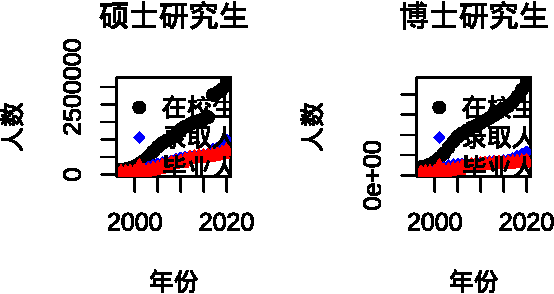
\includegraphics{sciguide_files/figure-latex/unnamed-chunk-7-1} \caption[中国硕士博士研究生录取、毕业与在校人数变化]{中国硕士博士研究生录取、毕业与在校人数变化}\label{fig:unnamed-chunk-7}
\end{figure}

前面说了研究生的供给端,下面看看需求端也就是教职的变化,这里只考虑博士,因为当前教职对学历的要求已经比较高了。同样看来自教育部的数据,由于本科生从1999年开始扩招,教职数也一直增加。不过,高级职称的增加速度明显低于教职总数的增加速度而中级职称教职在快速增加。同时,从年龄分布上看,当前教职年龄高峰在 55\textasciitilde59岁,大概是二十年前大学扩招时入职的。如果退休年龄没有明显推迟的话,那么在10年内应该可以看到一个因为退休高峰导致的教职空缺期。10年内什么年龄段的人会博士毕业呢?大概是当前的本科生,考虑到本科4年加硕博连读6年,每个高校都有义务在学生刚接触高等教育或研究时给他们能实时吸纳研究进展的教学大纲,否则要是学生10年前选了小灵通网络优化专业,那么等到博士毕业基本就只有转行了。

\begin{Shaded}
\begin{Highlighting}[]
\CommentTok{\# 数据来自教育部}
\NormalTok{faculty }\OtherTok{\textless{}{-}} \FunctionTok{read.csv}\NormalTok{(}\StringTok{\textquotesingle{}data/faculty.csv\textquotesingle{}}\NormalTok{, }\AttributeTok{check.names =}\NormalTok{ F)}
\NormalTok{faculty2 }\OtherTok{\textless{}{-}}\NormalTok{ faculty[faculty}\SpecialCharTok{$}\NormalTok{category }\SpecialCharTok{==} \StringTok{\textquotesingle{}Total\textquotesingle{}}\NormalTok{, ]}

\FunctionTok{par}\NormalTok{(}\AttributeTok{mfrow=}\FunctionTok{c}\NormalTok{(}\DecValTok{1}\NormalTok{,}\DecValTok{2}\NormalTok{))}
\FunctionTok{plot}\NormalTok{(faculty}\SpecialCharTok{$}\NormalTok{year[faculty}\SpecialCharTok{$}\NormalTok{category }\SpecialCharTok{==} \StringTok{\textquotesingle{}Total\textquotesingle{}}\NormalTok{],faculty}\SpecialCharTok{$}\NormalTok{total[faculty}\SpecialCharTok{$}\NormalTok{category }\SpecialCharTok{==} \StringTok{\textquotesingle{}Total\textquotesingle{}}\NormalTok{],}\AttributeTok{pch=}\DecValTok{19}\NormalTok{, }\AttributeTok{main=}\StringTok{\textquotesingle{}教职数\textquotesingle{}}\NormalTok{,}\AttributeTok{ylim=}\FunctionTok{c}\NormalTok{(}\DecValTok{0}\NormalTok{,}\FunctionTok{max}\NormalTok{(faculty}\SpecialCharTok{$}\NormalTok{total)),}\AttributeTok{xlab =} \StringTok{\textquotesingle{}年份\textquotesingle{}}\NormalTok{, }\AttributeTok{ylab =} \StringTok{\textquotesingle{}人数\textquotesingle{}}\NormalTok{)}
\FunctionTok{points}\NormalTok{(faculty}\SpecialCharTok{$}\NormalTok{year[faculty}\SpecialCharTok{$}\NormalTok{category }\SpecialCharTok{==} \StringTok{\textquotesingle{}Professors\textquotesingle{}}\NormalTok{], faculty}\SpecialCharTok{$}\NormalTok{total[faculty}\SpecialCharTok{$}\NormalTok{category }\SpecialCharTok{==} \StringTok{\textquotesingle{}Professors\textquotesingle{}}\NormalTok{],}\AttributeTok{pch=}\DecValTok{18}\NormalTok{,}\AttributeTok{col=}\StringTok{\textquotesingle{}blue\textquotesingle{}}\NormalTok{)}
\FunctionTok{points}\NormalTok{(faculty}\SpecialCharTok{$}\NormalTok{year[faculty}\SpecialCharTok{$}\NormalTok{category }\SpecialCharTok{==} \StringTok{\textquotesingle{}Asso. Professors\textquotesingle{}}\NormalTok{],faculty}\SpecialCharTok{$}\NormalTok{total[faculty}\SpecialCharTok{$}\NormalTok{category }\SpecialCharTok{==} \StringTok{\textquotesingle{}Asso. Professors\textquotesingle{}}\NormalTok{],}\AttributeTok{pch=}\DecValTok{17}\NormalTok{,}\AttributeTok{col=}\StringTok{\textquotesingle{}red\textquotesingle{}}\NormalTok{)}
\FunctionTok{points}\NormalTok{(faculty}\SpecialCharTok{$}\NormalTok{year[faculty}\SpecialCharTok{$}\NormalTok{category }\SpecialCharTok{==} \StringTok{\textquotesingle{}middle\textquotesingle{}}\NormalTok{],faculty}\SpecialCharTok{$}\NormalTok{total[faculty}\SpecialCharTok{$}\NormalTok{category }\SpecialCharTok{==} \StringTok{\textquotesingle{}middle\textquotesingle{}}\NormalTok{],}\AttributeTok{pch=}\DecValTok{15}\NormalTok{,}\AttributeTok{col=}\StringTok{\textquotesingle{}orange\textquotesingle{}}\NormalTok{)}
\FunctionTok{legend}\NormalTok{(}\StringTok{\textquotesingle{}topleft\textquotesingle{}}\NormalTok{,}\AttributeTok{legend =} \FunctionTok{c}\NormalTok{(}\StringTok{\textquotesingle{}总数\textquotesingle{}}\NormalTok{,}\StringTok{\textquotesingle{}教授\textquotesingle{}}\NormalTok{,}\StringTok{\textquotesingle{}副教授\textquotesingle{}}\NormalTok{,}\StringTok{\textquotesingle{}中级职称\textquotesingle{}}\NormalTok{), }\AttributeTok{col =} \FunctionTok{c}\NormalTok{(}\StringTok{\textquotesingle{}black\textquotesingle{}}\NormalTok{,}\StringTok{\textquotesingle{}blue\textquotesingle{}}\NormalTok{,}\StringTok{\textquotesingle{}red\textquotesingle{}}\NormalTok{,}\StringTok{\textquotesingle{}orange\textquotesingle{}}\NormalTok{),}\AttributeTok{pch=}\FunctionTok{c}\NormalTok{(}\DecValTok{19}\NormalTok{,}\DecValTok{18}\NormalTok{,}\DecValTok{17}\NormalTok{,}\DecValTok{15}\NormalTok{))}

\NormalTok{col }\OtherTok{=}\NormalTok{ RColorBrewer}\SpecialCharTok{::}\FunctionTok{brewer.pal}\NormalTok{(}\DecValTok{8}\NormalTok{,}\StringTok{\textquotesingle{}Set2\textquotesingle{}}\NormalTok{)}
\FunctionTok{plot}\NormalTok{(faculty2}\SpecialCharTok{$}\NormalTok{year,faculty2}\SpecialCharTok{$}\StringTok{\textasciigrave{}}\AttributeTok{30 Years \& Under}\StringTok{\textasciigrave{}}\NormalTok{,}\AttributeTok{pch=}\DecValTok{19}\NormalTok{, }\AttributeTok{main=}\StringTok{\textquotesingle{}教职数\textquotesingle{}}\NormalTok{,}\AttributeTok{ylim=}\FunctionTok{c}\NormalTok{(}\DecValTok{0}\NormalTok{,}\DecValTok{110000}\NormalTok{),}\AttributeTok{xlab =} \StringTok{\textquotesingle{}年份\textquotesingle{}}\NormalTok{, }\AttributeTok{ylab =} \StringTok{\textquotesingle{}人数\textquotesingle{}}\NormalTok{,}\AttributeTok{col=}\NormalTok{col[}\DecValTok{1}\NormalTok{])}
\FunctionTok{points}\NormalTok{(faculty2}\SpecialCharTok{$}\NormalTok{year,faculty2}\SpecialCharTok{$}\StringTok{\textasciigrave{}}\AttributeTok{31{-}35years}\StringTok{\textasciigrave{}}\NormalTok{,}\AttributeTok{pch=}\DecValTok{18}\NormalTok{,}\AttributeTok{col=}\NormalTok{col[}\DecValTok{2}\NormalTok{])}
\FunctionTok{points}\NormalTok{(faculty2}\SpecialCharTok{$}\NormalTok{year,faculty2}\SpecialCharTok{$}\StringTok{\textasciigrave{}}\AttributeTok{36{-}40years}\StringTok{\textasciigrave{}}\NormalTok{,}\AttributeTok{pch=}\DecValTok{17}\NormalTok{,}\AttributeTok{col=}\NormalTok{col[}\DecValTok{3}\NormalTok{])}
\FunctionTok{points}\NormalTok{(faculty2}\SpecialCharTok{$}\NormalTok{year,faculty2}\SpecialCharTok{$}\StringTok{\textasciigrave{}}\AttributeTok{41{-}45years}\StringTok{\textasciigrave{}}\NormalTok{,}\AttributeTok{pch=}\DecValTok{15}\NormalTok{,}\AttributeTok{col=}\NormalTok{col[}\DecValTok{4}\NormalTok{])}
\FunctionTok{points}\NormalTok{(faculty2}\SpecialCharTok{$}\NormalTok{year,faculty2}\SpecialCharTok{$}\StringTok{\textasciigrave{}}\AttributeTok{46{-}50years}\StringTok{\textasciigrave{}}\NormalTok{,}\AttributeTok{pch=}\DecValTok{14}\NormalTok{,}\AttributeTok{col=}\NormalTok{col[}\DecValTok{5}\NormalTok{])}
\FunctionTok{points}\NormalTok{(faculty2}\SpecialCharTok{$}\NormalTok{year,faculty2}\SpecialCharTok{$}\StringTok{\textasciigrave{}}\AttributeTok{51{-}55years}\StringTok{\textasciigrave{}}\NormalTok{,}\AttributeTok{pch=}\DecValTok{13}\NormalTok{,}\AttributeTok{col=}\NormalTok{col[}\DecValTok{6}\NormalTok{])}
\FunctionTok{points}\NormalTok{(faculty2}\SpecialCharTok{$}\NormalTok{year,faculty2}\SpecialCharTok{$}\StringTok{\textasciigrave{}}\AttributeTok{56{-}60years}\StringTok{\textasciigrave{}}\NormalTok{,}\AttributeTok{pch=}\DecValTok{12}\NormalTok{,}\AttributeTok{col=}\NormalTok{col[}\DecValTok{7}\NormalTok{])}
\FunctionTok{points}\NormalTok{(faculty2}\SpecialCharTok{$}\NormalTok{year,faculty2}\SpecialCharTok{$}\StringTok{\textasciigrave{}}\AttributeTok{61 Years \& Over}\StringTok{\textasciigrave{}}\NormalTok{,}\AttributeTok{pch=}\DecValTok{11}\NormalTok{,}\AttributeTok{col=}\NormalTok{col[}\DecValTok{8}\NormalTok{])}
\FunctionTok{legend}\NormalTok{(}\StringTok{\textquotesingle{}topleft\textquotesingle{}}\NormalTok{,}\AttributeTok{legend =} \FunctionTok{c}\NormalTok{(}\StringTok{\textquotesingle{}30岁以下\textquotesingle{}}\NormalTok{,}\StringTok{\textquotesingle{}30{-}34\textquotesingle{}}\NormalTok{,}\StringTok{\textquotesingle{}35{-}39\textquotesingle{}}\NormalTok{,}\StringTok{\textquotesingle{}40{-}44\textquotesingle{}}\NormalTok{,}\StringTok{\textquotesingle{}45{-}49\textquotesingle{}}\NormalTok{,}\StringTok{\textquotesingle{}50{-}54\textquotesingle{}}\NormalTok{,}\StringTok{\textquotesingle{}55{-}59\textquotesingle{}}\NormalTok{,}\StringTok{\textquotesingle{}60岁以上\textquotesingle{}}\NormalTok{), }\AttributeTok{col =}\NormalTok{ col,}\AttributeTok{pch=}\FunctionTok{c}\NormalTok{(}\DecValTok{19}\NormalTok{,}\DecValTok{18}\NormalTok{,}\DecValTok{17}\NormalTok{,}\DecValTok{15}\NormalTok{,}\DecValTok{14}\NormalTok{,}\DecValTok{13}\NormalTok{,}\DecValTok{12}\NormalTok{,}\DecValTok{11}\NormalTok{))}
\end{Highlighting}
\end{Shaded}

\begin{figure}
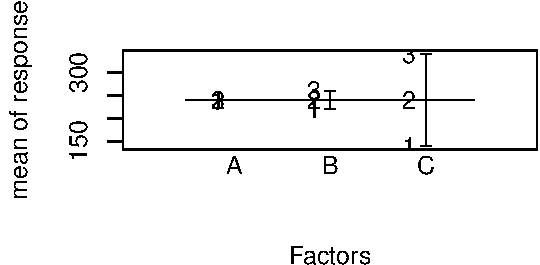
\includegraphics{sciguide_files/figure-latex/unnamed-chunk-8-1} \caption[中国不同教职人数变化及年龄构成]{中国不同教职人数变化及年龄构成}\label{fig:unnamed-chunk-8}
\end{figure}

除了退休带来教职的空缺外,教职数也在扩增。每年的教职数一直在稳定增长,但成长空间不算大,别忘了博士毕业生数可是逐年增长的,所以以后熬年限评职称是肯定不行的,目前30-34岁这个年龄段的教职人数在快速上升而前一个年龄段的人数并不多也比较稳定,这说明取得教职大概率是而立之年之后的事。这种较长的培养年限显著区别于其他行业,因为很多行业从业人员进入30-34岁基本进入了中层,而从事教职这个年龄刚刚入行。
这些年新增的教职数基本稳定在2万这个水平,但最近几年显著增加,2019年与2020甚至超过3万。同期每年新增博士毕业生超过6万而录取数超过了10万,也就是说,教职市场在今后可预期的时间里撑死也就能解决一半博士毕业生的就业问题,另外一半肯定要转行。

总之,目前博士研究生会长期面临毕业延期问题,同时教职市场的增长也无法消化当前的毕业生,需要同时考虑非教职的就业。

\hypertarget{ux5b66ux672fux804cux4e1aux8defux5f84}{%
\subsection{学术职业路径}\label{ux5b66ux672fux804cux4e1aux8defux5f84}}

全国博士毕业生目前在几万人的水平,按照很多人的说法,读到博士就应该去做学术。但学术路径可能并不好走,简单划分,学术路径包括以下几个阶段:

\begin{itemize}
\item
  博士博后阶段,主要目标累积文章拿教职,占当年博士毕业生 30\%
\item
  独立课题组阶段,主要目标能自己课题组正常运行,占当年博士毕业生 5\%
\item
  学术带头人阶段,主要目标其平台或方向可以持续运行,占当年博士毕业生 1\%
\item
  学科带头人阶段,主要目标是为自己学科从国家那边争取资源,占当年博士毕业生 0.1\%
\end{itemize}

下面是一个图表,可用来评估不同阶段的状态。

\begin{longtable}[t]{lllll}
\caption{\label{tab:unnamed-chunk-9}理想学术路径}\\
\toprule
指标 & 博士博后 & 独立课题组 & 学术带头人 & 学科带头人\\
\midrule
年产文章 & 1 & 2 & ~10 & >10\\
文章档次 & 专业期刊 & 一超多强 & 综述 & CNS\\
年龄 & 32 & 35 & 45 & 70\\
规模 & 1 & <10 & 20-30/有梯队 & 50-100/有传承\\
课程 & 带学生 & 本科研究生教学 & 学位培养计划 & 学科前沿指导\\
\addlinespace
会议 & 口头报告 & keynote & 分会场主席 & 大会报告\\
职称 & 讲师/研究员 & 副教授 & 教授 & 学生教授\\
期刊 & 审稿人 & 编委 & 副主编 & 主编\\
帽子 & 百篇优博 & 百人/优青/青千 & 长江/杰青/千人 & 院士\\
年新增人数/总人数 & 10万/100万 & 2000/50万 & 500/2万 & 50/2000\\
\addlinespace
基金/年审批数目 & 青基 /20000 & 面上 /20000 & 重点 /1000 & 重大 /个位数\\
行政 & 跑腿 & 自给自足 & 院系领导 & 院长校长\\
\bottomrule
\end{longtable}

如果成为院士(中国科学院/中国工程院)算学术巅峰的话,那么院士的选拔可以看作到达顶峰的路径。选拔方法是什么呢?两年一次,一次总共大概 150 人,工程科学对半分,平均一年 75 人。我们假定若干年后每年还是 75 人,因为两院院士总规模这么些年并未有很大规模的变化,就算加上文科一级教授也就是 100 这个数量级。那么若干年后竞争这个数的人选平均看大概都是同年级的博士同学。目前每年全国土鳖博士毕业生 6 万多人,算上海归,同一年龄组大概 7 万人应该比较合理。也就是说,你需要在同年级博士毕业生里成为千分之一左右的精英才算有希望成为院士级别的学者。

另一个算法可以用博导数量估计,毕竟每个博士背后都有一个博导。那么全国博导能有多少呢,乐观估计 6 万,年龄分布从 35 岁到 65 岁,如果是均匀分布的话且保证 65 岁退休,那么每年能产生出 2 千正高岗位,除以当年大约 7 万的博士人数,这个比例不到百分之三。就算我把那些做学术但不培养博士的岗位算上,这个比例也不会超过 5\%。硕士毕业生 15 年大概 50 万,说明副高大概最多也就这个数,每年也就 1-2 万岗位,也就是说大概 20\% 的博士最终能走到副高,其实这个比例也不算高,不过可以作为大多数人可以预想的目标。而副高里其实也就四分之一的人是真正可以独立科研的,其余的都是小老板,有自己独立课题组的人占当年毕业生的比例都是 5\% 以下。

也就是说,留在学术界的博士里面大部分人最后都是没法继续攀爬到学术带头人甚至独立课题组的。或者错过了年龄,或者需要照顾家庭,这才是常态,绝大部分博士止步副高二十年是很正常的事,上面那条学术路径只适合千分之一的人走完。所以说选了科研的很多人最后会有副业或其他重心,通过咨询、培训与职业化路径例如教书、律师、医生还有工程师来实现社会价值与自我价值,在前沿努力的科学家固然可敬,但机会总数固定后人数增加就会造成人才外溢。

你可能会说做学术要有一定理想,不能这么功利,说这话的有相当比例站着说话不腰疼。如果你已经走到教授研究员这个档次自然可以跟人谈理想,但坦白说现在的博导平均拿到学位都是 20 年前的事了,那个时候博士一年毕业 7 千多人,而现在博士毕业生数目翻了 10 倍,换句话在目前的晋升条件下你成为教授的概率大概是 50\%,如果有一半不做学术,几乎可以肯定就是教授了。10 年前一年博士毕业人数大概是现在的一半多,这意味着其晋升教授可能性也有十分之一,尚算合理。但 10 年后如果博士年毕业生达到 10 万,那么其成为教授将跟现在成为优青差不多难度,代际不平衡是十分严重的。不了解基础状况就把人往坑里带的后果挺严重的,自上而下,金字塔顶端人数就那么多,一味扩大底端几乎意味着大量博士要陷入无尽的博后循环之中去拉伸等级。

所以其实我挺理解很多劝博士毕业转行的看法的,哪怕你手握博士学位,目前在国内想走到独立课题组也是个5\%概率的事,大概 20 个人里有一个。考虑到一般博士同学同院系大概也就是 20 个人,如果学术水平不在前面,基本可以重新考虑下人生规划了,因为此时你选择科研就真的需要兴趣激发了,不然身边的落差会折磨你几十年。而且上面的估计有个严重的问题,那就是大量使用了均匀分布,但真实的情况却是极不均匀分布,你的师承关系跟毕业院校都会把这个分布搞得更加极端,而且后发者优势在科研里面非常常见,但前面的坑都满了你怎么让后发者上?

同时要注意,国内博士毕业生人数还在不断上升,一方面说明教职还是有空间的,另一方面则暗示了今后博士毕业生生存环境将会更加恶劣,竞争会更加激烈。同时,目前教职数目会逐渐趋稳,如果你没赶上新学科新方向的窗口期大爆发,基本就是始终要接纳这个竞争强度了,只会更强不会更弱。而且有些研究方向必然因为学科发展走向没落,没必要跟一伙老气横秋的人抱团取暖,该转方向就转,反正大家都没基础。

同时我们看一下美国,美国生物医药博士最终走上常任轨的比例大概 7-15\%,另外那些人并不是人间蒸发,而是去了业界做研发(R\&D)、中间人(产品支持、技术支持、销售、科学写作等)、运营(制造业、分析人、产品经理等)、商业(融资、投资等)以及法律相关行业(专利、技术转移等)。这个比例比国内要低,也就是转行对于美国博士而言是正常的职业选择,也是为社会输送人才的重要途径。我们将在本书最后一章详细讨论转行的职业选择问题。

读博转行可能也是个好事,早点把青春奉献到知识洼地去才更能实现自己的价值,相比学术界科研,业界科研可能是一个很好的选择,毕竟能磕下博士学位,搞点别的也应该没啥问题。博士及后面的博后阶段可以很好锻炼自己的专业技能并正确评价自己,通过投稿开会获取业内同行人脉联系并掌握面向社会寻求资源解决问题的能力,这种对自己了解对业内有认可且向外界拿许可的经历在各行各业都是相通的,关于怎么转换技能与额外的就业技能我们会在第九章讨论。

同时,如果选择了科研道路也要知道上面的概率,当不成分子也可以先做分母,心态上说服自己静下心来做科研就可以了,乐在其中则何乐不为?切不可惶惶不可终日,空费时光。

\hypertarget{ux5168ux6808ux79d1ux5b66ux5bb6}{%
\subsection{全栈科学家}\label{ux5168ux6808ux79d1ux5b66ux5bb6}}

当前研究生培养的一个短板就是综合性不强,或者说自嘲为科研民工,走出自己专业就不太敢想了,理想的研究生则应对不懂的部分也有自信,最终能攒出一个结果,而这个结果可能要同时用到多学科技术,即使没学过,也要会找到合作的人。反观当前研究生教育,选课都很保守,不是自己以后研究领域的东西不选或直接让导师选,非常被动。打比方我设计一个算法,效果不错,但问题是别人不会用,那么就应该把算法打包成函数甚至设计一个简易图形界面让明白用途但不想理解算法的人用。但这个过程就不能靠分工了,得有人全流程都明白并进行整合,这种综合性有点类似工程师思维,甲方是同行,你得让同行解决实际问题而不是看你炫技术。基础学科肯定是有发展空间的,但目前基础学科要解决的问题已经都很像工程问题了,所以这类综合能力的问题化聚焦是研究生很重要的竞争力,痴迷于单一技术而看不到要实际解决的科学问题培养的只能是齿轮化的专家而不是科学家。

很多人觉得大学负责通识教育与精英教育,研究生要更多关注技能培训成为所谓专家,我觉得这可能是科研民工思想的源头。现状是通识教育与精英教育从来都不如标准化的技能培训有吸引力,虽然可能潜力更高,这导致培养出的专家视野总是有局限性,需要在团队里合理配置才会提高解决问题的效率。例如想成为生物医药领域 PI(Principal Investigator) 的研究生博后要在 10 年内搞出 8 篇一作才有戏,越来越长时间的专家培养是不可避免的趋势。

同时,专家在团队里并不总是起正面效用,分工促进效率在面对可分解为具体步骤的行业或学科是好使的,但面对真实问题例如实验研究,实验者与数据处理者是不能脱节的。这里团队中指望两拨人放下成见平等交谈是很不现实的,因为占据理论高度的数据处理者或者说统计学家总会觉得做实验的是啥都不懂的;实验科学家则会对基于各种假设的模型忧虑重重,感觉缺少实证。你不可能不湿鞋就过河,不了解实验具体操作就在那边对实验设计指指点点只会让实验者与统计学家的隔阂越来越大。

所以我觉得解决实际问题需要培养全栈科学家,就是那种从采样到样品分析再到数据分析都有概念的科学家,即使以后实验可以外包也必须要进行所谓脏活的训练,数据科学家需要洗数据,全栈科学家可能连样品都要亲自采集,纸上谈兵绝对不行,养出一堆赵括天天跟你扯术语用的对不对完全就是浪费资源,全部开掉完全不影响进度,他们只是想通过凸显自己的专业性来找面子,根本就不打算解决问题。职业化的一个问题在于其整体是为了构建一个利益共同体求生存,科学问题则是项目化的,并不需要行政官僚层级结构来维系利益,很多时候找来的专家钱没少拿但问题没解决还内部互相指责对方不了解自己的专业术语,这才是现代科研中的大问题。

现在的研究生要有意识地训练自己成为全栈科学家,就算以后不做科研了,对实际问题解决的全流程理解也会让你很容易转行并与其他领域的人交流。更重要的是,这是所谓团队领导力的重要能力基础,几乎所有行业都对管理层培养有着基层轮岗的要求,公务员、医生、厨师、工程师还有律师等行业精英的训练过程都有着严格的全流程培训要求,搞空降或许会带来创新,但不了解步骤的空降几乎都是灾难。所以科研人员可以依赖专业人员,但心里要有问题解决的路线图与原理层的认识。不要过分依赖专家,他们都是为自己发声,只有你自己为你的项目负责,被专家牵着鼻子走对全栈科学家是一种耻辱,保证兼听则明就可以了。

专业的人喜欢谈差异与术语,解决问题的人更关注问题背后的共性。而统计学家也不要拿起实验设计不够随机与混杂因素工具变量啥的一堆术语去居高临下教育别人,这些问题要是都解决了一个 t 检验不就天下太平了,还需要统计学家做什么?扎根实际问题然后抽象出可测量的统计量,然后在模型中进行控制或考察,让结果具有可比性与重复性才是更重要的。不能固步自封,因为新技术一直在出现,新理念也一直在出现,自己不懂就去打击是很幼稚的行为。

\hypertarget{ux53efux91cdux590dux6027ux5371ux673a}{%
\section{可重复性危机}\label{ux53efux91cdux590dux6027ux5371ux673a}}

可重复性危机是当前科研领域里最大的问题,如果结论不可被重复验证,那么科学性就无从谈起。这里我们先讨论科研里通用假设检验的问题,然后讨论下规律性,最后介绍应对这个危机的可重复性研究与开放科学趋势。

\hypertarget{ux96f6ux5047ux8bbeux663eux8457ux6027ux68c0ux9a8cnhst}{%
\subsection{零假设显著性检验(NHST)}\label{ux96f6ux5047ux8bbeux663eux8457ux6027ux68c0ux9a8cnhst}}

零假设显著性检验(NHST)则是可重复性危机的核心。NHST 更常见的形式是 p 值,也就是在零假设成立的条件下某事件发生的概率。打个比方,我们从一个混合了黑白两种颜色小球的口袋里有放回的取一个小球三次,结果都是白球。这里我们设定零假设为黑球白球各一半,那么发生三次白球的概率为12.5\%,这个不算极端。但是,如果有放回取了十次,结果还是都是白球,这情况发生概率大概为千分之一,这就比较极端了。在此基础上,我们有理由认为零假设不成立,而此时就需要一个阈值来帮助我们判断是否成立,目前学术界会认为5\%或0.05的概率可以作为显著性与否的阈值。科研中我们会去计算零假设下出现当前实验结果的概率,也就是p值,如果低于阈值就可以认为是极端事件就拒绝零假设而高于阈值则认为零假设下可能发生。

当然,我们现在科研用的p值还会考虑零假设之外的备择假设,如果拒绝了零假设就转而接受备择假设。不过一旦引入备择假设就需要讨论错误,这里我们把决策出的结果分为阴性与阳性,而事实分为真假。零假设为真但接受了备择假设的情况,这就是假阳性或者第一类错误;零假设为假但没拒绝零假设就是假阴性或者第二类错误。这里我们可以看到第一类错误与前面设定的决策阈值密切相关,如果设定在5\%或者0.05,那么我们就有5\%的可能性做出了错误判断。第二类错误则与统计功效也就是真阴性的概率有关,通常会设定在80\%,如果功效过低,例如10\%,那么犯第二类错误的概率就很高。举例来说,我脚43码的但我不知道,这时去买鞋别人问我脚尺码我说44码的其实是错了,但不影响脚能穿进去,此时尺码的区别功效就不足。但如果我穿久了就会发现确实是大了,此时相当于我通过多次实验或采样提高了统计功效,但可能这个差别虽然明显但也不影响穿。通常NHST关心第一类错误,但设计实验会考虑第二类错误,通过提高样本量来提高统计功效。

p 值有多流行呢?根据 Jeff Leek 的\href{https://docs.google.com/presentation/d/1hzdSDaPPSE9xUYZHhOVfQIRPPdwe0A9SdE7QDsK3bOA/edit\#slide=id.g255a5ace66_3_796}{估计},如果把 p 值当成一篇文献,那么其被引次数已经超过 300 万次了,当之无愧的史上被引次数之王,甩\href{http://www.nature.com/news/the-top-100-papers-1.16224}{第二名}一个数量级。原因其实很简单,p 值已经渗透到几乎所有学科的研究中了,特别是实验学科。可想而知,如果产生 p 值的 NHST 出了问题其影响力有多大。下面谈下 NHST 具体的问题:

如果一个假设对另一个假设来说很稀少,NHST 会在很低的条件概率下拒绝掉,然后那些稀少的事情在 NHST 里就成了无法被检验的事情。这个例子最早是 Cohen \href{http://ist-socrates.berkeley.edu/~maccoun/PP279_Cohen1.pdf}{提出}用来说明人们在使用 NHST 时的问题。零假设是某人是中国人,备择假设是非中国人。我们知道张三是人大代表的概率大概是百万分之二,这是个事实。不过这个事实在零假设里很难发生,备择假设里也无法发生。零假设我们拒绝了某人是中国人,那么根据 NHST,他不是中国人。但问题是人大代表一定要是中国人,此时就会出现事实跟NHST矛盾的情况。在此类问题里,NHST 永远无法认定稀有事件,也就是功效永远不足,并会给出错误答案。

这个问题本质上是多数人在使用 p 值时搞混了条件概率,拿上面人大代表的例子来说,我们的假设 H0 在面对张三这个数据 D 时给出了拒绝 \(p(H0|D) = 0\),这个决定是构建在假设 H0 成立时出现 D 的概率太低(即 \(p(D|H0)\))之上,也就是说 NHST 下,我们默认下面的概率是成立的:

\[
p(D|H_0) = p(H_0|D)
\]
如果你修过任何基础的统计学课程都会知道这两个概率之间差了一个贝叶斯公式。通过使用贝叶斯定理,在新数据出现后原有概率是要被更新而不是直接拒绝掉的。p 值给的是前者,要想知道随机生成的概率,需要知道零假设为真的概率。通俗点说就是 NHST 属于革命派,不认可就打倒你;贝叶斯属于改良派,用新的证据更新原有理论。这个问题的本质就是把假设下的事实与事实下的假设搞混导致的,这是 NHST 的一个致命问题,然而致命问题可不止这一个。

过去的一百年,测量方法的精度是在不断提高的,而精度其实又会影响研究结果,很不幸,也是通过 NHST 来进行的。其实 NHST 在实验物理学里用的还是好好的,例如我去检测一个物理量,只有数据出现在其理论预测下数值四五个标准差以外才会对理论产生实质作用。此时,测量精度越高,由于测量误差导致的对原有理论的冲击就会越少,因为物理学的预测性要比化学生物等学科要好不少且此时 NHST 检测的原有理论是比较真实的。但在其他学科,特别是心理学跟医学的控制实验里,在实验开始前你几乎就可以确定零假设是不成立的,要不然你也没必要分组,此时你去搞 NHST ,几乎一定可以找到差异,此时测量精度如果不断上升,那么你会识别到一系列差异,但这些差异的效果是无法体现在p值里的,p值可能非常小,但效应却属于明显但很微弱,这样的结果也许可以发表,但对实际问题的解决几乎没有贡献。更极端的情况是如果你加大了样本量来提高统计功效,你总是能发现差异的,也就是你的零假设里原有学科理论为真也是会被方法学进步给推翻的。总结下就是 Meehl 在60年代就提出的\href{https://philpapers.org/rec/MEETIP}{悖论}:方法学的进步与增大样本数对于相对硬(理论根基深厚)的学科证伪是正面的,但对相对软(理论比较模糊)的学科则是弱化。方法学悖论的根基其实是应用学科与基础学科的矛盾,基础学科用 NHST 检验观察事实中的理论,但应用学科用 NHST 来检验的是实验设计预测下的事实,此时实验设计的那个假设与 NHST 的零假设并不对应,而 NHST 先天弱化零假设的问题就凸显了。

事实上,p 值正在成为测量投资与努力而不是事实的标准,给定差异,我们总能找到足够的样本来发现这个差异(这也就是前面说的功效分析)。也就是说,NHST 有时候功效不足测不到差异,有时候又一定会能测出差异,但科学事实并不会因为你使用了 NHST 而发生变化,特别是有意义的变化。而作为标准的 p 值其实在被样本数决定同时又综合了测定效果强度与不确定性,这样的一个标准其实有点多余,你完全可以用描述性统计与置信区间来分别表示效果强度与不确定性。同时,p 值也并不能增加新知识,考虑一个多元线性模型,我们只能在多元模型里得到参数,也就是有限检验,不能发现未知参数,但科学就是寻找未知;变量间的关系在数值改变后如何考察,正负关系如何预测,预测性也就无法实现。那么此时还有必要使用 NHST 吗?

20 世纪的技术有了意义深远的进步,但更现实的问题是,科研里低垂果实已经没有了,学科从分立走向交叉,服务社会职能的出现要求科学家回答的不再是科学问题而是现实问题,或者说,科学地回答现实问题。但现实问题非常复杂,科学家要想排除影响,大都采用控制实验与随机化来验证观察研究中的事实。注意,这里的事实不再是理论假设,而是一个现象,如果本来就观察到了差异,用 NHST 根本就不会让我们知道更多的事实,我们可以用无数独立手段证明这个事实的存在然后整合进学科知识体系,但并不能产生更多的思考,理论的预测效能在 NHST 里实际是体现不出来的。而预测效果不显著在 NHST 里还不能说明效果不存在,到这里 NHST 基本就成了鸡肋。

p 值还被一些人认为可以代表结果的可重复性,但重复性是统计功效的函数,跟 p 值无关,p 值不能传达真实与否的信息。统计功效很重要,跟样本数关系大当样本数增大时,空检验总会被拒绝,因此当零假设为感兴趣的理论时,样本数与准确性会提高理论强度,但零假设不存在时,样本数与准确性提高只会弱化理论。此外,p 值控制只考虑假阳性而不是假阴性,所以对假阴性有要求的实验也要慎重使用 p 值,但遗憾的是对很多研究人员而言搞清楚NHST已经不容易了,再去理解这里面的问题会被认为过于麻烦。

那么我们的控制实验里对无关因素的平衡与随机如何呢?显然,平衡掉不随机的部分需要你事先知道这部分是什么,很遗憾,目前科研特别是基于观察的研究并不能事先知道,有时候就是想发现这些不知道自己不知道的东西。这种情况下基于 p 值或零假设的假设检验其实是不应该用的,打个比方,你发现观测数据中 A 基因与甲疾病相关,但究竟是不是 A 基因引发甲疾病还是需要用控制变量来验证的,很有可能 A 基因与甲疾病同样被 B 基因调控,但你根本就没测 B 基因,所以研究本身就是不完整的。

那么通过组学技术等先进分析手段把知道的不知道的一起去测不就完整了吗?也不是,当你测量数量增加时,假设检验的个数也增加了,此时你的 p 值阈值如果是 0.05,那么 10000 个测量变量中会有 500 个即使随机测定都会出现差异的基因。去年有人建议把 p 值阈值设到 0.005,但 p 值这个问题,重要的不是把 0.05 降到 0.005,通用阈值这个想法太偷懒,应该让研究人员充分理解 p 值实际意义与使用方法,毕竟在有些研究领域控制错误发现率后阈值实际比 0.005 \href{http://www.nature.com/news/one-size-fits-all-threshold-for-p-values-under-fire-1.22625}{低得多},改变阈值只是把需要核实的数量减少了,虽然这也有一定意义。举个例子,10000 个基因中有一个是真实的,你测定后按照 0.05 发现了 501 个,按照 0.005 发现了 51 个,也就是说需要验证的数量减少了。但真实研究中,你会遇到 0.05 发现了 501 个但 0.005 只发现了 50 个的情况,真实差异由于效应量或造成的差异量不够大而被你的决策方法给漏掉了。甚至也会出现 0.05 发现了 480 个而 0.005 只发现了 48 个的情况。也就是说,当你观察的问题效应不大时,p 值有可能不管怎么调整都无法发现。这个锅不在 p 值,在于你要研究的效应效应太低而你用了不恰当的研究方法与假设来检验这个现象。这类效应大小问题就是 type M 型错误,这里M代表数量级,只要你假设检验的效应总是介于有无之间,这个问题就很难规避。

同时,当你进行条件控制时,其实又掉到了高维诅咒的坑里。打比方我做了一组实验,最后发现某种药在 A 条件 B 参数面对 C 人群中 D 年龄分组里是有效的。那么问题来了,假设 ABCD 全是互斥的二元变量,那么我这个结果实际上是做了\(2^4 = 16\)次对比得到了一次显著性结果。然而,如果我们采用 p 值,那么 16 次随机假设检验里出现一次 p 值小于 0.05 的概率是\(1-(1-0.05)^{16} = 0.56\),也就是说这个结果在完全随机状态下也有高于一半的概率可能会发生。那么这个结论是否可靠呢?其实跟 p 值没关系,最终是跟样本量挂钩,如果你的满足条件的目标样本很大,那这个结果很可能就是对的。相反,如果这个结果是来自于小样本,虽然根据多元模型是显著的,但具体到这个条件下其实就几个样本,此时结果就不能算靠谱。

探索性数据分析通常会面对这个无穷假设困境,当你不断引入协变量后,维度的增加导致样本实际是稀疏欠拟合的,最后看到现象可能就是假象。发现的价值在这里也不依赖 p 值,依赖效果大小与参数,进一步依赖样本量。不过条件控制中也要考虑因果关系,否则单纯增加特征值可能并不好提高模型的性能。高维诅咒实际还连着多重比较的坑,多次比较后 p 值是可以校正后继续用的,不过这里套的坑是无穷假设,也就是说当你比较的次数多时,有效应也看不出来了,这就要求对数据本身的结构有深入了解。当前在错误率控制上也有很多校正方法,当然也是对 p 值的校正,所以批评声从来也没断过。

现在只能相信强结论,也就是说无论你用哪种统计方法去进行检验,这个现象都是客观存在的,不会因为决策方法的变化而出现结论差异。不过这个提法现在看还是太理想了,因为强结论真的很强或显而易见,现代科研也发展上百年了,基本也都发现了。如果一个现象足够强,p 值一定会发现,贝叶斯方法也一定会发现,此时不存在效应大小问题。但更多的事实或规律是埋藏在当前认为的随机或噪声之中的,我们的分析水平也就刚刚好能把疑似信号与噪声进行区分,而这个区分是否靠谱则完全成了迷,统计学在这里帮不上忙,技术进步倒成了关键。我看到一些研究寄希望于数据挖掘技术解决学科内现象发现问题,这里只能说对于显而易见但被忽视的现象是有帮助的,但对于高噪声数据,降低测量噪声对结论的帮助要远大于遴选能发现差异统计方法的努力。数据迷信会让你看到伪规律,而测量技术进步才会真的发现价值规律。

NHST 的另一个问题在于其本身表示不了效应的方向。p 值经常是双边概率取中间那一部分,所以当你看到一个很小的 p 值时,你并不知道这个效应的方向是更大还是更小,此时你还是需要去看效应值。在这个情况下,如果报道 p 值不报道效应,那么就好比我告诉你明天要变天但又不告诉你变成什么一样毫无意义。在多数实验设计中,变化几乎是一定存在的,例如我敲掉了某个基因去验证功能,基因的变化与功能肯定有区别,大都来源于观察实验,更有意义的是影响大小,这个大小更多需要专业判断而不是简单的 p 值。如果理科学生学了半天最后就知道用 p 值来判断结论,那么这个学位不给也罢。这类搞不清楚效应方向的问题是 type S 型错误,S代表符号,此时验证性实验特别需要注意。

NHST 还有个问题在于 p 值的选择性报道或者说发表歧视,研究人员通常会尝试大量的实验条件组合但发表的论文里只有那些有显著性的结果,这导致了科研文献不能准确反应研究现状。这不一定意味着结果是错的,如果这个实验条件具有广泛的数据支持而不是仅仅来自于模型推断的选择性报道,那么我们只能说推理上不严谨。不过,从这里我们可以看出,依赖 p 值来判断结果是存在问题的,而不使用 p 值,很多研究结果实际是无法简单报道的。然而,大量选择性报道可能出现一个副作用,论文的讨论很多是依赖引文,如果引文结果不靠谱,那么后续研究只有同样采用了选择性报道才能继续跟进发表,最后形成一种确认偏误,这情况比想象的要常见。甚至在系统综述过程中,对确认偏误的忽略可能通过结论影响决策者,那就成了一种自我实现。此时,进行综述的科学家可以通过数据的二次分析与整合来凸显那些本来由于样本量不够而忽略的现象。

另外一种隐性 p 值选择性报道是通过模型选择来实现的,不同的统计模型会产生不同的假设检验结果,研究人员通常只会报道那些有阳性结果的统计模型。这个非常难识别,因为统计模型通常比较复杂且研究人员有可能是先上船后买票,也就是先发现这个模型结果有利然后根据模型组织文章。这里面会牵扯到探索性数据分析与论证的差异,如果研究人员把新模型当成了文章亮点,那读者是完全看不出来这里面的不恰当行为的。此时还是要依赖数据公开,如果大家都能下载到数据,标准化后然后同时跑多个模型,只有共存结果才有可能可靠。不过,这里面的问题在于多个模型的假设是不一样的,只有符合数据本身统计特征的模型才能被加入到评价体系里。

关于 NHST 虽然问题一大把,但系统去看,p 值也有着自己的生命力,我想更多人关心的是如果我不用 NHST ,拿什么证明我的结果可靠?如果没得选,这剂毒药还是得吃啊。答案其实上面都大概提到了,你如果坚持使用 p 值,那么就也请同时报告参数估计与置信区间,虽然这个方法也被人喷过。如果你打算完全开一条新路,那就去学贝叶斯统计,贝叶斯统计有自己成套的处理体系,简单说就是先假设参数分布,然后用数据更新分布,后验分布计算出来就同时有点估计跟方差估计,同时多重比较问题也不存在,但随机错误无法避免,此时参数估计方差大也能体现,后续研究可以使用这次的后验数据作为下次先验数据,这样你可以实现完全的 N + 1 模式科研,其验证与预测性也很大程度依赖采样与模拟技术,之前贝叶斯方法不能流行很重要的一个原因就在于计算比较贵,现在就便宜很多了。

这次的危机能不能解决?什么时候解决?现在谁也不知道,但了解问题是解决问题的第一步,而路还很长。

\hypertarget{ux89c4ux5f8bux6027}{%
\subsection{规律性}\label{ux89c4ux5f8bux6027}}

从另一个视角看,可重复性危机的一个重点在于如何判断规律性。所谓规律性,本质在于数据中存在模式或者异质性,如果数据是均质的,那么要么是均匀分布,要么是噪声的正态分布。

前面提到的NHST的原版也就是Fisher那个没有备择假设的版本其实在应对规律性问题上是有点不一样的。在只有零假设的语境下,备择假设其实只是零假设所对应的可能性空间里的一种,只是出现概率比较低。换句话说,如果可能性空间里出现概率高,那么信息含量也就低,因此拒绝也没什么问题。同时,这里面也就不存在条件概率的问题,因为零假设包含了所有假设的可能性空间,数据是一定会支持零假设的。

不过在这个原版里,可能性空间的计算就不是很方便了。经典女士品茶那个实验里,其可能性空间为70种不同的猜测,只有八次猜测每次都猜对的概率是小于0.05的。如果猜的次数更多,那么在0.05这个阈值下其实可以允许犯错;反之,猜的次数少则实验本身的功效不足以发现规律。这里这个p值是穷举完可能性空间计算出的精确值而不是根据分布来算的,那么我们是否可以在保留数据不变的条件下去随机化分组,然后通过仿真模拟来判断是否存在规律性呢?

如果有规律的事实在实验限定的空间里发生,其p值的分布应该会与随机过程产生的p值不一样。这里我不打算采用多次随机抽样,因为此时分布事实上是已知的,此时进行随机实验其实是在假设分布存在且成立的条件下判断事实。相反,我会随机生成一组数据但保留这一组数据当成既成事实,但随机化分组过程来检验p值的分布,此时应该更符合事实存在后对假设的判断这个思路。这里我们考虑三种情况:

\begin{itemize}
\tightlist
\item
  真实差异固定
\item
  完全是随机数
\item
  固定的真实差异加上随机数
\end{itemize}

第一种情况是规律完全成立;第二种是完全无规律;第三种是可观察或可测量的数据。生成三组数据后我们对其分组(简单二分)进行10000次随机化操作,然后进行t检验,记录并观察p值。

\begin{Shaded}
\begin{Highlighting}[]
\FunctionTok{set.seed}\NormalTok{(}\DecValTok{1}\NormalTok{)}
\CommentTok{\# 真实差异}
\NormalTok{x }\OtherTok{\textless{}{-}} \FunctionTok{c}\NormalTok{(}\FunctionTok{rep}\NormalTok{(}\DecValTok{100}\NormalTok{, }\DecValTok{260}\NormalTok{), }\FunctionTok{rep}\NormalTok{(}\DecValTok{200}\NormalTok{, }\DecValTok{260}\NormalTok{))}
\CommentTok{\# 随机差异}
\NormalTok{xr }\OtherTok{\textless{}{-}} \FunctionTok{rnorm}\NormalTok{(}\DecValTok{520}\NormalTok{)}
\CommentTok{\# 考虑误差的真实差异}
\NormalTok{xm }\OtherTok{\textless{}{-}} \FunctionTok{c}\NormalTok{(}\FunctionTok{rep}\NormalTok{(}\DecValTok{100}\NormalTok{, }\DecValTok{260}\NormalTok{), }\FunctionTok{rep}\NormalTok{(}\DecValTok{200}\NormalTok{, }\DecValTok{260}\NormalTok{)) }\SpecialCharTok{+} \FunctionTok{rnorm}\NormalTok{(}\DecValTok{520}\NormalTok{)}
\NormalTok{p }\OtherTok{\textless{}{-}}\NormalTok{ pr }\OtherTok{\textless{}{-}}\NormalTok{ pm }\OtherTok{\textless{}{-}} \FunctionTok{c}\NormalTok{()}
\ControlFlowTok{for}\NormalTok{ (i }\ControlFlowTok{in} \DecValTok{1}\SpecialCharTok{:}\DecValTok{10000}\NormalTok{) \{}
        \CommentTok{\# 随机化分组}
\NormalTok{        g }\OtherTok{\textless{}{-}} \FunctionTok{factor}\NormalTok{(}\FunctionTok{sample}\NormalTok{(}\FunctionTok{c}\NormalTok{(}\DecValTok{1}\NormalTok{, }\DecValTok{2}\NormalTok{), }\DecValTok{520}\NormalTok{, }\AttributeTok{replace =}\NormalTok{ T))}
\NormalTok{        p[i] }\OtherTok{\textless{}{-}} \FunctionTok{t.test}\NormalTok{(x }\SpecialCharTok{\textasciitilde{}}\NormalTok{ g)}\SpecialCharTok{$}\NormalTok{p.value}
\NormalTok{        pr[i] }\OtherTok{\textless{}{-}} \FunctionTok{t.test}\NormalTok{(xr }\SpecialCharTok{\textasciitilde{}}\NormalTok{ g)}\SpecialCharTok{$}\NormalTok{p.value}
\NormalTok{        pm[i] }\OtherTok{\textless{}{-}} \FunctionTok{t.test}\NormalTok{(xm }\SpecialCharTok{\textasciitilde{}}\NormalTok{ g)}\SpecialCharTok{$}\NormalTok{p.value}
\NormalTok{\}}
\CommentTok{\# 显示中文}
\FunctionTok{library}\NormalTok{(}\StringTok{\textquotesingle{}showtext\textquotesingle{}}\NormalTok{)}
\FunctionTok{showtext\_auto}\NormalTok{()}
\FunctionTok{par}\NormalTok{(}\AttributeTok{mfrow =} \FunctionTok{c}\NormalTok{(}\DecValTok{1}\NormalTok{, }\DecValTok{3}\NormalTok{))}
\CommentTok{\# 展示真实差异t检验下p值的分布}
\FunctionTok{hist}\NormalTok{(}
\NormalTok{        p,}
        \AttributeTok{breaks =} \DecValTok{100}\NormalTok{,}
        \AttributeTok{main =} \FunctionTok{substitute}\NormalTok{(}\FunctionTok{paste}\NormalTok{(}\StringTok{\textquotesingle{}存在真实差异时\textquotesingle{}}\NormalTok{, }\FunctionTok{italic}\NormalTok{(}\StringTok{\textquotesingle{}p\textquotesingle{}}\NormalTok{), }\StringTok{"值分布"}\NormalTok{)),}
        \AttributeTok{xlab =} \FunctionTok{substitute}\NormalTok{(}\FunctionTok{paste}\NormalTok{(}\FunctionTok{italic}\NormalTok{(}\StringTok{\textquotesingle{}p\textquotesingle{}}\NormalTok{), }\StringTok{"值"}\NormalTok{)),}
        \AttributeTok{ylab =} \StringTok{\textquotesingle{}频率\textquotesingle{}}
\NormalTok{)}
\CommentTok{\# 展示随机差异t检验下p值的分布}
\FunctionTok{hist}\NormalTok{(}
\NormalTok{        pr,}
        \AttributeTok{breaks =} \DecValTok{100}\NormalTok{,}
        \AttributeTok{main =} \FunctionTok{substitute}\NormalTok{(}\FunctionTok{paste}\NormalTok{(}\StringTok{\textquotesingle{}不存在真实差异时\textquotesingle{}}\NormalTok{, }\FunctionTok{italic}\NormalTok{(}\StringTok{\textquotesingle{}p\textquotesingle{}}\NormalTok{), }\StringTok{"值分布"}\NormalTok{)),}
        \AttributeTok{xlab =} \FunctionTok{substitute}\NormalTok{(}\FunctionTok{paste}\NormalTok{(}\FunctionTok{italic}\NormalTok{(}\StringTok{\textquotesingle{}p\textquotesingle{}}\NormalTok{), }\StringTok{"值"}\NormalTok{)),}
        \AttributeTok{ylab =} \StringTok{\textquotesingle{}频率\textquotesingle{}}
\NormalTok{)}
\CommentTok{\# 展示考虑误差的真实差异t检验下p值的分布}
\FunctionTok{hist}\NormalTok{(}
\NormalTok{        pm,}
        \AttributeTok{breaks =} \DecValTok{100}\NormalTok{,}
        \AttributeTok{main =} \FunctionTok{substitute}\NormalTok{(}\FunctionTok{paste}\NormalTok{(}\StringTok{\textquotesingle{}存在真实差异与噪声时\textquotesingle{}}\NormalTok{, }\FunctionTok{italic}\NormalTok{(}\StringTok{\textquotesingle{}p\textquotesingle{}}\NormalTok{), }\StringTok{"值分布"}\NormalTok{)),}
        \AttributeTok{xlab =} \FunctionTok{substitute}\NormalTok{(}\FunctionTok{paste}\NormalTok{(}\FunctionTok{italic}\NormalTok{(}\StringTok{\textquotesingle{}p\textquotesingle{}}\NormalTok{), }\StringTok{"值"}\NormalTok{)),}
        \AttributeTok{ylab =} \StringTok{\textquotesingle{}频率\textquotesingle{}}
\NormalTok{)}
\end{Highlighting}
\end{Shaded}

\begin{figure}
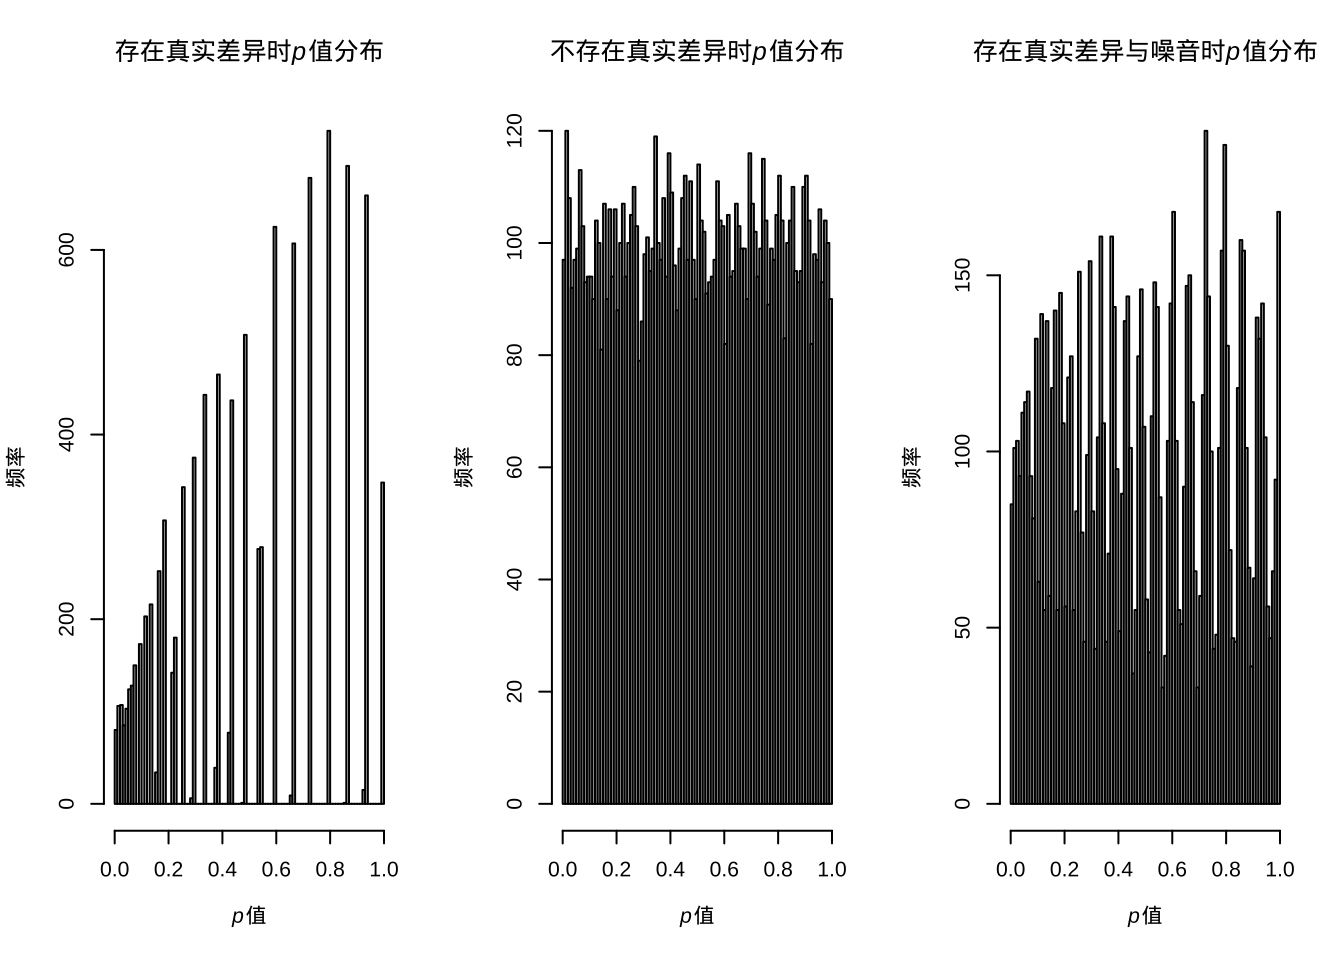
\includegraphics{sciguide_files/figure-latex/unnamed-chunk-10-1} \caption[p值在存在真实差异、不存在真实差异及同时存在真实差异与噪声的分布]{p值在存在真实差异、不存在真实差异及同时存在真实差异与噪声的分布}\label{fig:unnamed-chunk-10}
\end{figure}

这个结果非常有意思,第一个能看到的现象是如果数据本身存在规律性,那么p值的分布是一个离散分布。这个分布介于0到1之间,越接近0的部分越密集,越接近1的的部分越稀疏,但是如果计算小于0.05,0.5,0.9的比例情况,会发现这种稀疏分布依旧符合均匀分布的概率分布特征。如果数据不存在规律性,那么p值的分布就是很均匀的。如果数据混合了规律性与噪声,依然会显示出这种离散分布特征。下面我用qq图来观察下这个分布跟均匀分布的区别:

\begin{Shaded}
\begin{Highlighting}[]
\FunctionTok{set.seed}\NormalTok{(}\DecValTok{42}\NormalTok{)}
\CommentTok{\# 生成均匀分布}
\NormalTok{ref }\OtherTok{\textless{}{-}} \FunctionTok{runif}\NormalTok{(}\DecValTok{10000}\NormalTok{)}
\FunctionTok{par}\NormalTok{(}\AttributeTok{mfrow =} \FunctionTok{c}\NormalTok{(}\DecValTok{1}\NormalTok{, }\DecValTok{3}\NormalTok{))}
\CommentTok{\# 用分位图对比均匀分布与不同的p值分布}
\FunctionTok{qqplot}\NormalTok{(ref, p, }\AttributeTok{xlab =} \StringTok{\textquotesingle{}均匀分布\textquotesingle{}}\NormalTok{, }\AttributeTok{ylab =} \FunctionTok{substitute}\NormalTok{(}\FunctionTok{paste}\NormalTok{(}\StringTok{\textquotesingle{}存在真实差异时\textquotesingle{}}\NormalTok{, }\FunctionTok{italic}\NormalTok{(}\StringTok{\textquotesingle{}p\textquotesingle{}}\NormalTok{), }\StringTok{"值分布"}\NormalTok{)))}
\FunctionTok{qqplot}\NormalTok{(ref, pr, }\AttributeTok{xlab =} \StringTok{\textquotesingle{}均匀分布\textquotesingle{}}\NormalTok{, }\AttributeTok{ylab =} \FunctionTok{substitute}\NormalTok{(}\FunctionTok{paste}\NormalTok{(}\StringTok{\textquotesingle{}不存在真实差异时\textquotesingle{}}\NormalTok{, }\FunctionTok{italic}\NormalTok{(}\StringTok{\textquotesingle{}p\textquotesingle{}}\NormalTok{), }\StringTok{"值分布"}\NormalTok{)))}
\FunctionTok{qqplot}\NormalTok{(ref, pm, }\AttributeTok{xlab =} \StringTok{\textquotesingle{}均匀分布\textquotesingle{}}\NormalTok{, }\AttributeTok{ylab =} \FunctionTok{substitute}\NormalTok{(}\FunctionTok{paste}\NormalTok{(}\StringTok{\textquotesingle{}存在真实差异与噪声时\textquotesingle{}}\NormalTok{, }\FunctionTok{italic}\NormalTok{(}\StringTok{\textquotesingle{}p\textquotesingle{}}\NormalTok{), }\StringTok{"值分布"}\NormalTok{)))}
\end{Highlighting}
\end{Shaded}

\begin{figure}
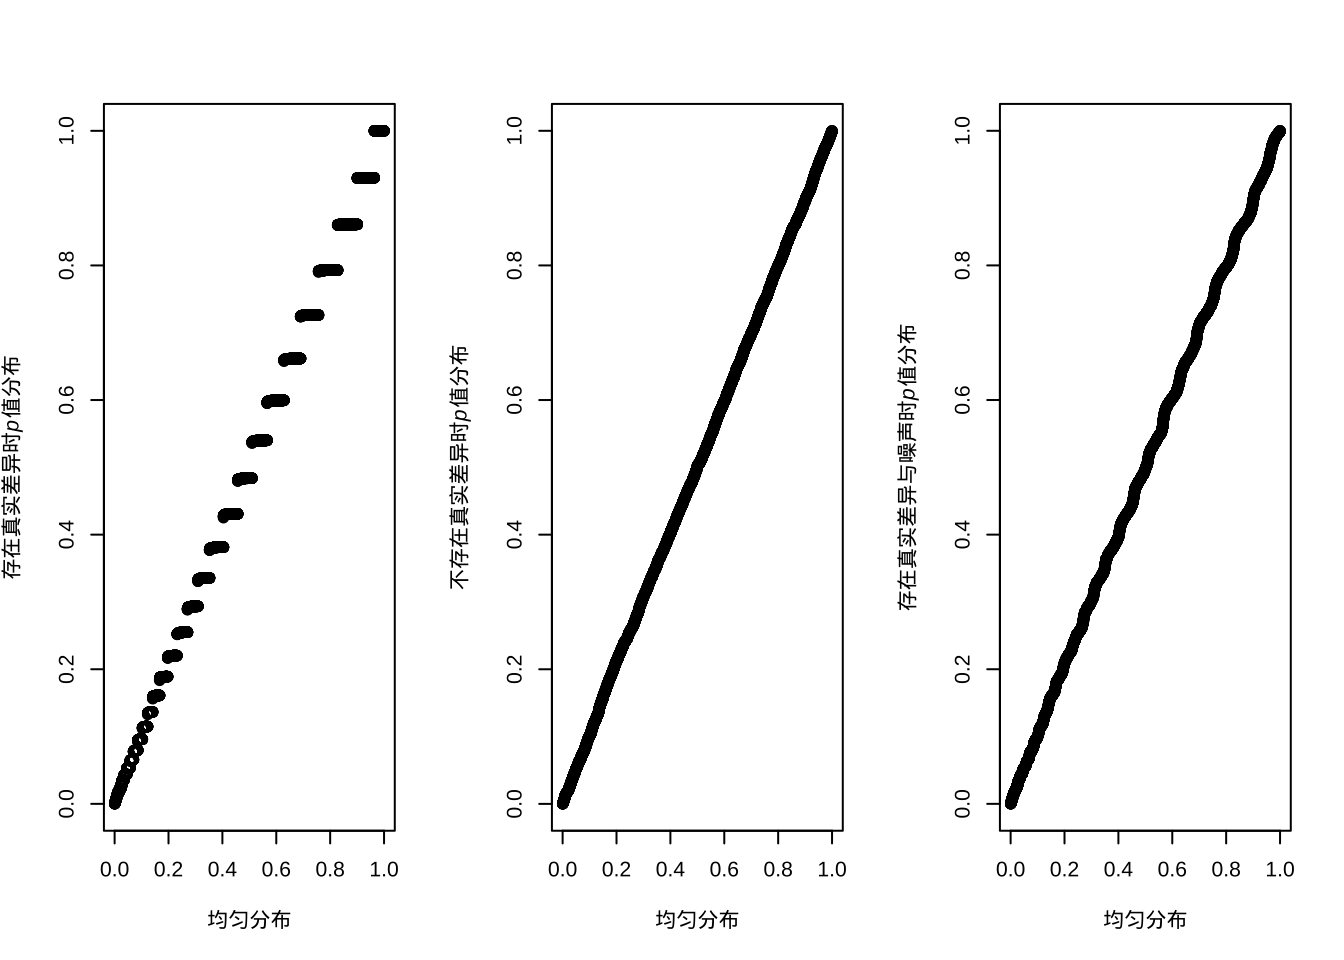
\includegraphics{sciguide_files/figure-latex/unnamed-chunk-11-1} \caption[分位图观察p值在存在真实差异、不存在真实差异及同时存在真实差异与噪声的分布跟均匀分布的区别]{分位图观察p值在存在真实差异、不存在真实差异及同时存在真实差异与噪声的分布跟均匀分布的区别}\label{fig:unnamed-chunk-11}
\end{figure}

可以看到,如果数据本身存在规律性,其随机化分组后的p值虽然跟均匀分布很接近,但qq图上确实会表现出前密后舒的螺旋延伸状态。这里为了区别我再做一个仿真,这次我不是对分组随机而是对采样随机:

\begin{Shaded}
\begin{Highlighting}[]
\FunctionTok{set.seed}\NormalTok{(}\DecValTok{1}\NormalTok{)}
\CommentTok{\# 固定分组}
\NormalTok{g }\OtherTok{\textless{}{-}} \FunctionTok{factor}\NormalTok{(}\FunctionTok{c}\NormalTok{(}\FunctionTok{rep}\NormalTok{(}\DecValTok{1}\NormalTok{, }\DecValTok{260}\NormalTok{), }\FunctionTok{rep}\NormalTok{(}\DecValTok{2}\NormalTok{, }\DecValTok{260}\NormalTok{)))}
\NormalTok{p }\OtherTok{\textless{}{-}} \FunctionTok{c}\NormalTok{()}
\ControlFlowTok{for}\NormalTok{ (i }\ControlFlowTok{in} \DecValTok{1}\SpecialCharTok{:}\DecValTok{10000}\NormalTok{) \{}
        \CommentTok{\# 随机化采样}
\NormalTok{        x }\OtherTok{\textless{}{-}}  \FunctionTok{sample}\NormalTok{(}\FunctionTok{c}\NormalTok{(}\FunctionTok{rep}\NormalTok{(}\DecValTok{100}\NormalTok{, }\DecValTok{260}\NormalTok{), }\FunctionTok{rep}\NormalTok{(}\DecValTok{200}\NormalTok{, }\DecValTok{260}\NormalTok{)) }\SpecialCharTok{+} \FunctionTok{rnorm}\NormalTok{(}\DecValTok{520}\NormalTok{), }\DecValTok{520}\NormalTok{)}
\NormalTok{        p[i] }\OtherTok{\textless{}{-}} \FunctionTok{t.test}\NormalTok{(x }\SpecialCharTok{\textasciitilde{}}\NormalTok{ g)}\SpecialCharTok{$}\NormalTok{p.value}
\NormalTok{\}}
\FunctionTok{par}\NormalTok{(}\AttributeTok{mfrow =} \FunctionTok{c}\NormalTok{(}\DecValTok{1}\NormalTok{, }\DecValTok{2}\NormalTok{))}
\FunctionTok{hist}\NormalTok{(}
\NormalTok{        p,}
        \AttributeTok{breaks =} \DecValTok{100}\NormalTok{,}
        \AttributeTok{main =} \FunctionTok{substitute}\NormalTok{(}\FunctionTok{paste}\NormalTok{(}\StringTok{\textquotesingle{}采样随机时\textquotesingle{}}\NormalTok{, }\FunctionTok{italic}\NormalTok{(}\StringTok{\textquotesingle{}p\textquotesingle{}}\NormalTok{), }\StringTok{"值分布"}\NormalTok{)),}
        \AttributeTok{xlab =} \FunctionTok{substitute}\NormalTok{(}\FunctionTok{paste}\NormalTok{(}\FunctionTok{italic}\NormalTok{(}\StringTok{\textquotesingle{}p\textquotesingle{}}\NormalTok{), }\StringTok{"值"}\NormalTok{)),}
        \AttributeTok{ylab =} \StringTok{\textquotesingle{}频率\textquotesingle{}}
\NormalTok{)}
\FunctionTok{qqplot}\NormalTok{(ref, p, }\AttributeTok{xlab =} \StringTok{\textquotesingle{}均匀分布\textquotesingle{}}\NormalTok{, }\AttributeTok{ylab =} \FunctionTok{substitute}\NormalTok{(}\FunctionTok{paste}\NormalTok{(}\StringTok{\textquotesingle{}采样随机时\textquotesingle{}}\NormalTok{, }\FunctionTok{italic}\NormalTok{(}\StringTok{\textquotesingle{}p\textquotesingle{}}\NormalTok{), }\StringTok{"值分布"}\NormalTok{)))}
\end{Highlighting}
\end{Shaded}

\begin{figure}
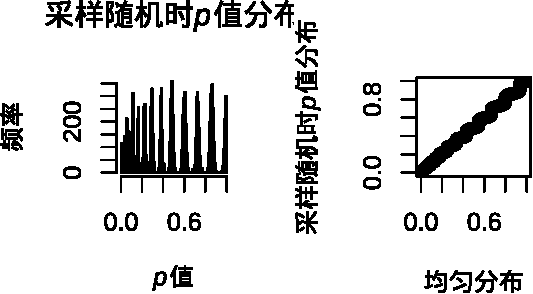
\includegraphics{sciguide_files/figure-latex/unnamed-chunk-12-1} \caption[采样随机时p值的分布与均匀分布的分位图]{采样随机时p值的分布与均匀分布的分位图}\label{fig:unnamed-chunk-12}
\end{figure}

这里我们同样能看到这种蛇形走位,而且似乎随机化样品看到的趋势更明显。但同样的,这里模拟逻辑还是保持数据不变,只是随机化过程。

这个规律性数据的p值分布可能对实验学科非常有意义。如果规律会造成数据异质性而我们的分组过程就是试图发现这种规律性,那么不可避免的会在p值分布上造成离散分布的状态。相反,随机相关则不会呈现出这种p值的离散分布而是均匀分布。这个均匀与离散分布的差异如果能用一个统计量来描述,那么我们事实上就能根据这个统计量区别出真实规律与随机相关。

在这个语境下,我们就不用搞这些多重检验下p值的阈值矫正了,直接对每一次假设检验进行分组随机化模拟过程,然后生成p值分布。如果其对应分布统计量表示为离散均匀分布,那么这一组假设检验的规律性就是有保证的,如果指示为均匀分布,那么这组数据本身就可以判定为无法检测规律而排除。这样我们可以对数据在进行统计推断前做一个规律性测试,只有通过了规律性测试的数据才值得进行统计推断。而且,只要单次统计推断给出小于0.05的p值,我们就可以直接相信,因为那些可能出现随机相关的数据已经被我们排除掉了。

当然,这个方法可能只适用于多重检验语境下可重复性危机,也仅对存在离散分布规律的数据有用,不过这种源于 Fisher 的基于模拟的精确检验思想也许会在计算模拟比较容易的今天推广到更多的应用场景里。

\hypertarget{ux53efux91cdux590dux6027ux7814ux7a76}{%
\subsection{可重复性研究}\label{ux53efux91cdux590dux6027ux7814ux7a76}}

实验结果的可重复性研究不是个新鲜概念,上个世纪就开始有讨论了,最早是心理学,现在已经蔓延到多个学科。但可重复性研究的流程其实比想象的要复杂,完整的可重复性研究包含多个步骤,例如人群可重复性、科学问题是否一致、假设是否一致、实验设计是否一致、实验人员是否一致、数据分析流程是否一致、代码是否可公开、推断的合理性与结论是否一致。新闻里常说的可重复性不好主要是最后一项结论的差异,但整体流程的任何一个环节都可能出问题。不同学科对可重复性的要求也并不一致,实验学科如果是验证简单体系要求会特别高,例如理论物理,而复杂体系考察综合指标要求就可能降到结果数量级上可重复就可以了,例如环境痕量污染物的分析,因为样品前处理复杂待测物含量经常逼近检出限,此时要求很高的可重复性意义不大而含量数量级通常就能反映足够的环境信息。下图是一个常见的可重复性研究需要考虑的步骤,想完整重现别人的研究需要对方提供每一步的信息。

\begin{figure}
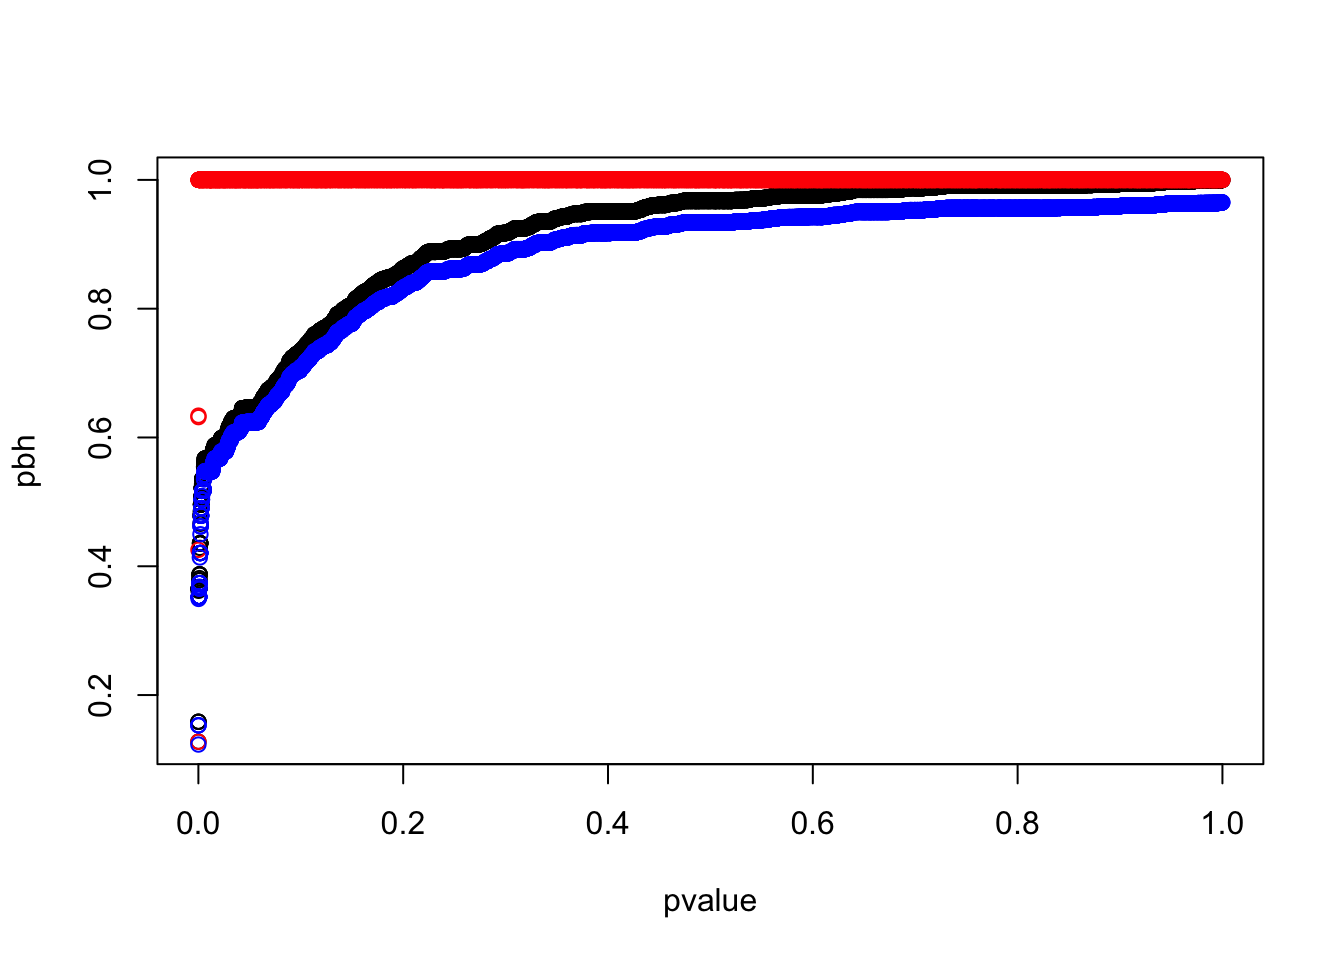
\includegraphics{sciguide_files/figure-latex/unnamed-chunk-13-1} \caption[可重复性研究的步骤]{可重复性研究的步骤}\label{fig:unnamed-chunk-13}
\end{figure}

不过,狭义的可重复性研究仅关心数据产生后步骤的可重复性,包括但不限于原始数据共享与数据处理代码共享。当前很多学科的期刊都开始要求论文作者共享原始数据,这是一个很好的起点,但更重要的是数据分析步骤。科研用图形化界面软件的流行降低了科研数据分析的门槛,但因为大多数软件并不同时提供用户数据分析的脚本,一个副作用就是使数据分析重现变得很困难。从科研角度来看,保证数据分析的透明度很关键,因此现代科研人员应该花时间去掌握一门高级编程语言,在公布论文的同时也公布论文中分析推断的生成源码,这样既方便自己的成果传播也提高了研究可信度。从原始数据到成果这一阶段的可重复性是应该开放给整个学术圈进行检验的,这样机制的存在会使可重复性效果低的研究成果能被快速排除而不是消耗资源去验证一个数据处理问题,毕竟也很少有基金是支持验证别人研究成果的。

NHST 是科研可重复性危机的核心,但科学家的人性也不可忽视。科学本身是构建在错误校正过程上的,但科学家评价却是人性化的,良好的评价很多时候成了科学家追求的标的。不论是对影响因子的追求还是学术明星的打造,非科学的评价与评优其实影响到了科研结果的报道。科学家正在作为一个团体来维护自己的利益与社会地位,其副作用就是对失败的低容忍度,年龄限制与成果限制使得探索必须要符合效率原则,很多年轻人在年富力强的时候做了大量排列组合而非探索性的工作来确保个人的生存无虞,这样造成的损失目前我们无法衡量。随之伴生的学术不规范、不端与造假则是层出不穷,很多人开始利用一些规则上的漏洞来实现非科研目的,例如审稿流程与评优。科学家的形象要由团体的文化来体现,阳光底下没有新鲜事,除了开放获取的研究成果,研究整体流程也应该实现透明化,这样可以很大程度防止暗箱操作。

流程透明的开放科学趋势也是一种正在流行的解决方案。所谓流程透明,指的是从基金申请到修改到进度报告到结题报告到文章的投稿接受与后续跟进研究及评优都要有公开的记录可以查询,文书都要经过版本控制方便返溯,所有研究人员都要实名负责对应的项目。学术团体接受公众舆论监督与同行监督,日常学术交流也要有公开的记录与反馈机制,所有的记录不直接对外公开但接受实名查询并留存查询记录。这样透明化的流程可以保证学术团体除了发表论文之外还有其他的结果展示途径,进而避免实验结果的选择性汇报与资源的过度集中。打破自我包装与人脉对科研的束缚,让结果更直白地展示给所有人。此外,关于可重复性,Nature 就近年来的科研可重复性危机采访了五组科学家,分别从认知、NHST、FDR、数据共享与范式转化的角度进行了\href{https://www.nature.com/articles/d41586-017-07522-z}{论述},值得一读。在医疗领域也有了一些有意思的讨论,例如认为基于人群的归纳式诊断会被个性化精准医疗所替代,此时可重复性里内含的平均律就会被彻底颠覆,分子水平的因果逻辑可能成为未来的主要知识探索方向。预印本、开放获取与审稿、科研社交媒体及数据共享等新\href{https://theoreticalecology.wordpress.com/2019/01/22/tree-species-richness-and-its-effects-on-productivity-neither-global-nor-consistent/}{趋势}也孕育着新的问题解决方法。

\hypertarget{ux63a0ux593aux6027ux671fux520a}{%
\section{掠夺性期刊}\label{ux63a0ux593aux6027ux671fux520a}}

为了迎合行业内职称评定与论文发表需求,很多商人盯上了学术期刊出版这个产业。在学术期刊的出版流程中,出版商可以利用同行评议机制招募免费的审稿人,然后打着开放获取的名义向投稿人收取版面费。由于很多期刊只有线上版,他们只需要雇佣一名专职编辑来处理稿件就可以完整运行一份学术期刊,甚至他们还盯上了预印本服务器的稿件来解决稿源问题,通过向作者发信咨询投稿意向来钓鱼,这样的运作几乎可以看成空手套白狼的教科书版商业模型。著名的\href{https://beallslist.net/}{Beall's List} 收集了大量这样的出版集团名单,虽然2017年后已经不再更新但依旧可以拿来参考。

值得注意的是,现在很多掠夺性期刊存在洗白的趋势。他们会去联系一些学者给予主编副主编的职位,然后也确实有同行评议流程与论文发表,收费也不是特别夸张,个别期刊甚至能不断正反馈摆脱掉掠夺性期刊的过往。出现这个情况一方面是搞科研的还是太善良,另一方面则是他们利用了一些学术会议等营销手段弄假成真,此时想识别这类期刊要考察其发文量,一年少于10篇的新期刊基本可以认定为有洗白嫌疑的掠夺性期刊。

同时,几大传统科研论文出版集团为了争夺优质稿源,目前也在构建各自的期刊档次,争取把尽可能多的稿件留在自己的出版物内。很多大出版商的商业行为,例如雇佣高学历专业编辑而非找资深学术研究人员来担任主编副主编、期刊间层层转投的潜规则还有不断开办新期刊来接受新学科论文等都是有明确的营利性目的的。这种商业竞争一方面打击了老牌期刊依赖关系网收``水文''导致期刊质量口碑下降的现象,另一方面也因为专业化运营的高收费被很多人诟病。

很多人投稿只认老牌期刊其实是不愿放弃经营多年的圈内关系网,而另一些人则是看不惯高昂的收费。但对于年轻科研人员而言,很多比较新的领域与研究方向确实是收到一定排挤的,新期刊也确实给了他们发声渠道,这个应该属于学术界正常的新陈代谢。作为后来者,投稿时确实要注意这些出版界的趋势与学术评价的不同偏好,眼光可以长远些,只要做的内容足够有意义,期刊的平台影响其实不大,但一定要规避掠夺性期刊。

\hypertarget{ux8bbaux6587ux516bux80a1ux5316}{%
\section{论文八股化}\label{ux8bbaux6587ux516bux80a1ux5316}}

如果你去论文数据库搜严新气功,会发现很多经过同行评议的学术期刊发表了这类气功对某些生命过程影响的研究。估计审稿人还以为拼音写的严新气功是某种新药,不过这倒也说明了职业化科研有时候看重形式或程序合逻辑而忽略了背后的内容,算是某种八股化的表现。

现在的研究论文往往是存在某种套路的,完成了第一篇,后面就可以照着模版来写。这种八股化的论文适合刷文章与引用,但学术价值不高。很多人很喜欢这类论文,主要是因为容易写,不用动脑子,按着元素周期表搞排列组合就可以。这类文章在材料跟中药学里常见,真正做到了换汤不换药。

毋庸置疑,研究论文确实存在表述接近的可能,但八股文的出现更多是为了写论文而写论文的结果,深层次是成果考核的需求。很多八股文可以合并为一篇但偏要拆成一个物质一篇去刷数量,文章的意义更多是所谓填补空白而不是创新。论文八股化最需要的是对科学问题的明确,可以尝试解决一个当前不存在未来可能出现的问题,但很多论文描述的问题几乎永远不可能存在甚至根本就是类似气功的虚假问题。没有科学性的论文,即使同行评议漏过了也应该即使发现并撤掉。

\hypertarget{ux516cux4f17ux79d1ux5b66}{%
\section{公众科学}\label{ux516cux4f17ux79d1ux5b66}}

现代社会里除了职业科学家,也存在进行公众科学(Citizen Science)研究的公民科学家。公众科学是相对20世纪前绅士科学而言的,那时候做科学研究主要是有钱有闲的人的爱好。但工业化现代社会虽然通过精细分工抬高了职业化科研的门槛,但也因为技术进步降低了很多研究的门槛,这就有了公众科学。公众科学项目指需要公众参与的科学项目,经常也有职业科学家指导,项目对专业技能要求不高,一般是做数据采集整理还有简单的展示分析。因为门槛低,所以可以吸引到民间科学爱好者,项目集中在天文学与生态学领域。

公众科学经常可以为职业科研提供大量一手观察数据,反过来也算一种科普教育手段及启发式探索手段。伴随传感器、互联网与数据科学技术的普及,很多民间发现事实上也达到了相当的专业水准,很多科研人员还会借鉴这些通用技术来应用到自己的研究中。现代社会需要构建公民科学家与职业科学家交流的机制,及时吸取民间智慧而不是傲慢排斥来自民间的发现。

不过,有时候其实很难区分公众科学跟民科,后者又称为科妄,用来指代没有受过专业训练又热衷于研究的科学家。在《西方伪科学种种》一书里,马丁·加德纳认为民科的两大显著特点就是隔绝同行信息与妄想症。但这毕竟是20世纪的民科,现代社会的民科已经不再停留在永动机还有水变油这类一看就有问题的研究上了,很多民科接受过正规的训练,甚至发表过通过同行评议的论文,但其理论实在是太过玄幻无法验证。民科的最大问题在于有理论但不严谨论证,喜欢似是而非的解释而非严格的定性定量考察,如果能给予恰当的指导而不是简单嘲讽也能作为公众科学的领导者。

科学的世界没有东西之分。很多人会简单把西方的理论认为是高级的先进的科学的然后去批判东方的所有理论,但读过科学史就会发现西方世界也从来不缺民科,放血疗法顺势疗法跟中医比也就是半斤八两。科学知识有其边界,并不能现在就解释所有的现象,反而是很多现在看似用简单理论解释的现象后来被很多新的知识更新。有些非职业科学家最大的问题就在于搞研究的同时还打算传播不相关的价值观,想做好公众科学可能更重要的不在于知识传播而是科学思维的传播。

\hypertarget{ux79d1ux666e}{%
\section{科普}\label{ux79d1ux666e}}

科普是科学家传播科学知识与思维的重要途径。因为绝大多数人不进行科研,就算进行科研其很多科学背景知识也是中学水平的,所以现代社会中科普主要面向知识背景是义务教育或普通高中毕业水平。即使取得大学毕业文凭的现代人可能学了某个学科或专业,但另外的学科知识最理想也是停留在高中阶段,有些则因为文理分科等历史问题停留在义务教育阶段。这部分知识需要思考推理的部分不多,主要是了解事实本身与交流用的语言,形成背景概念。科普工作相当重要的一部分是填补初中与高中背景知识,这点中学老师做的可能要比所谓职业做科普的还要好。

科普另一部分内容是反应前沿科研成果的,但此时服务对象的背景知识水平因为有其他专业知识的支撑变得更高,同时受众也会相应收窄。面向专业人员的成果传播通常是N+1模式,也就是读者知道了N,你只需要把多出来的1说明白就可以了。但是,科普前沿成果要从零开始或者1开始,也就是说在介绍进展前要把背景意义都说清楚还要控制好难度。这种科普作品对读者要求不高但对作者要求非常高,科研人员自己写容易写成面向同行的报告而让中学老师来写又会大概率超出其知识水平。经常看到一些打着科普名号的文章只是堆砌专业术语然后给一大堆英文参考文献,读者不明觉厉就把作者封神追捧,这样的科普跟传教没多大区别。科普的第一要务就是要把事情讲清楚讲明白,既不是讲故事(因为很多结论是暂时的)也不是搞怪耍宝娱乐大众,更不能是高高在上语焉不详靠神秘感提高专业感。

伴随现代社会高等教育的普及,对前沿科研成果的需求会越来越多,这也把科普推到了职业化阶段。不论知识科普还是前沿科普都受益于信息技术进步,很多交互式或者多媒体科普方式的效果是明显好于文字效果的,社交网络的传播与营销方法成了职业科普作者的必修内容。不过,科普与知识普及最大的区别还在于科学精神,这点反而在现代社会的科普中有所缺失,越来越多的所谓科普作品过分强调了知识性故事性趣味性逻辑性但掩盖了科学探索中的探索性与不确定性。现代社会与现代人喜欢秩序、完美结局与确定性但科学探索却是概率的、打破常规的还有不断试错证伪的且结论都是暂时的,做科普要是无法调和科学精神与读者预期而倒向后者,那么无异于用信仰的方式来传播科学知识,这本身就是荒诞的。

\hypertarget{ux79d1ux5b66ux95eeux9898}{%
\section{科学问题}\label{ux79d1ux5b66ux95eeux9898}}

前面一直在说科学问题,这里就给出当前的问题列表。其实,2005年《科学》杂志提出了 100 个科学\href{https://science.sciencemag.org/content/309/5731/78.2}{问题}而中国关心的科学问题由中国科协筹集,每年发布。以下为当前列表:

\begin{itemize}
\tightlist
\item
  超高精度量子惯性导航技术
\item
  空间天气的及时准确预报
\item
  岩石圈构造应力场及其作用过程
\item
  煤矿重特大灾害智能报警方法与技术
\item
  工程结构安全的长期智能监测预警技术
\item
  城市交通基础设施智能协同运营技术
\item
  基于北斗卫星和5G通信技术的新型高速铁路列车运行控制技术
\item
  高原高寒冻土地区高速铁路与公路修建关键技术
\item
  跨深大海峡通道(悬浮隧道)关键技术
\item
  面向未来交通的路网全感知技术
\item
  时速 1000 公里及以上低真空管道运输高速磁悬浮铁路建造关键技术
\item
  未来城市地下交通及物流系统
\item
  航天运输技术难题
\item
  飞机级系统架构设计及仿真技术
\item
  面向工程应用的高精度动态测量
\item
  高效长寿命低成本电化学电力储能技术
\item
  海洋生态系统储碳与全球变化
\item
  脆弱生境生物多样性的维持机制
\item
  高水平放射性废物安全处置
\item
  绿色安全高效的低成本制氢技术
\item
  川藏铁路建设难点
\item
  未来全球能源互联网的关键技术
\item
  绿色农药创新研究和原创性靶标的发现
\item
  固态有机废弃物生物转化及其资源梯级利用
\item
  植物工厂人工环境条件下植物的生长发育调控
\item
  基于核酸物质的基因精准调控与医药技术
\item
  细胞命运决定机制的研究
\item
  人类智能的基因调控机理
\item
  全球变化对动物的影响及应对
\item
  植物对逆境的记忆功能与进化
\item
  DNA 存储技术
\item
  意识读取的前沿问题和关键技术
\item
  遗传信息的结构编码------纳米尺度遗传信息动态结构解析
\item
  记忆的物理化学基础
\item
  单分子化学反应动态过程的可视化
\item
  超临界场强的量子电动力学效应
\item
  宇宙中重元素的起源
\item
  极端条件下的可控燃烧
\item
  高性能热电材料
\item
  纳米纤维的产业化生产关键技术
\item
  核能系统高安全结构材料
\item
  高活性可见光催化材料
\item
  人工智能技术与新型智能复合材料的深度融合
\item
  类脑计算
\item
  新一代认知物联网关键技术
\item
  抗量子密码算法设计
\item
  大规模共享无人载运工具的协同智动管控仿真
\item
  工业互联网中数据集成和边缘处理技术
\item
  人与机器的情感交互
\item
  肿瘤转移机制与抗肿瘤转移新药研发
\item
  老年性痴呆的机制解析及诊治难点
\item
  精神疾病的新型治疗方法
\item
  免疫微环境分子分型及免疫治疗耐药机制
\item
  人机共融关键技术
\item
  微腔中的力光量子传感
\item
  高性能动力电池研发技术
\item
  新一代智能制造系统
\item
  基于多源信息融合的大型复杂系统健康状态监测与评估
\item
  人工智能在智能驾驶工程技术开发中的应用
\item
  先进微纳机器人技术
\item
  暗物质是种能探测到的基本粒子吗
\item
  对激光核聚变新途径的探索
\item
  单原子催化剂的催化反应机理
\item
  高能量密度动力电池材料电化学
\item
  情绪意识的产生根源
\item
  细胞器之间的相互作用
\item
  单细胞多组学技术
\item
  废弃物资源生态安全利用技术集成
\item
  全智能化植物工厂关键技术难题
\item
  近地小天体调查、防御与开发问题
\item
  大地震机制及其物理预测方法
\item
  原创药物靶标发现的新途径与新方法
\item
  中医药临床疗效评价创新方法与技术
\item
  人工智能系统的智能生成机理
\item
  氢燃料电池动力系统
\item
  可再生合成燃料
\item
  绿色超声速民机设计技术
\item
  重复使用航天运输系统设计与评估技术
\item
  千米级深竖井全断面掘进技术
\item
  海洋天然气水合物和油气一体化勘探开发机理和关键工程技术
\item
  冠状病毒跨种传播的生态学机制是什么?
\item
  引力波将如何揭示宇宙奥秘?
\item
  地球物质是如何演化与循环的?
\item
  第五代核能系统会是什么样子?
\item
  特种能场辅助制造的科学原理是什么?
\item
  数字交通基础设施如何推动自动驾驶与车路协同发展?
\item
  调节人体免疫功能的中医药机制是什么?
\item
  植物无融合生殖的生物学基础是什么?
\item
  如何优化变化环境下我国水资源承载力,实现健康的区域水平衡状态?
\item
  如何建立虚拟孪生理论和技术基础并开展示范应用?
\item
  如何开发新型免疫细胞在肿瘤治疗中的新途径与新技术?
\item
  水平起降组合动力运载器一体化设计为何成为空天技术新焦点?
\item
  如何实现农业重大入侵生物的前瞻性风险预警和实时控制?
\item
  信息化条件下国家关键基础设施如何防范重大电磁威胁?
\item
  硅光技术能否促成光电子和微电子的融合?
\item
  如何解决集成电路制造工艺中缺陷在线检测难题?
\item
  无人车如何实现在卫星不可用条件下的高精度智能导航?
\item
  如何在可再生能源规模化电解水制氢生产中实现``大规模''``低能耗''``高稳定性''三者的统一?
\item
  如何突破进藏高速公路智能建造及工程健康保障技术?
\item
  如何突破光刻技术难题?
\end{itemize}

这份列表其实更侧重技术面,也有基础理论的问题,但更多是融合了技术与原理的缝合怪问题,需要多学科协作来攻关。如果你的研究方向在这份列表中,那么应该不会有失业问题。

\hypertarget{thought}{%
\chapter{思维工具}\label{thought}}

这一章会侧重科学研究中比较重要的思维工具,但绝大多数讨论还是来自科学哲学。了解科学哲学的发展后再去了解下数学思维在数学史中的变化,毕竟原理能否数学化是判断科学学科是否成立的重要标准。不同于数学思维,接下来的统计思维则是科研中最通用的一种方法论而基于抽象能力的模型思维则是现代科研必不可少的重要工具。本章最后会讨论启发法,这大概是在信息不充分条件下最重要的科研思维工具。

\hypertarget{ux79d1ux5b66ux601dux7ef4}{%
\section{科学思维}\label{ux79d1ux5b66ux601dux7ef4}}

虽然做科研一般都不讨论哲学,太多形而上的东西,说也说不清道也道不明还无法证伪。但懂一点科学哲学还是很有必要的,不然很容易研究着研究着就会觉得自己做的东西是垃圾,是谋生的工具,虽然从某个角度看也没错,但科学哲学无疑是应对这种心态最好的心灵老鸭汤。

首先,哲学是解决人与世界关系的学问,而科学在词源(scientia)上是知识学问的意思,追求的是正确的东西或真理。哲学很多时候与哲学史等同,提的问题几乎万古长存,各流派解读的保质期也很久,因为没法验证也就不存在伪的可能。科学跟科学史或者说博物学就完全不同,是一种探索自然的理性精神,很多知识会被更新,了解科学史会更博学但并不增加科学知识本身,因为对于一件事科学上的描述几乎唯一。当我们认为自然是可知的时候,科学就是探索其原因原理的认识方式并提供方法工具。

科学方法论构建于三个基础之上:观察或实验、数学还有逻辑工具。观察与实验要做到可重复、可比及随机;数学提供量化评价工具;逻辑工具包括不限于归纳演绎、分类类比、公理化及假说演绎。科学提供的一定是系统性规律性的知识,任何学科如果没有自己的理论系统、数学模型与验证都只能算知识或经验,谈不上科学化的学科。科学哲学主要关注哲学史里跟科学相关的世界观、认识论与方法论。

\hypertarget{ux53e4ux5e0cux814a}{%
\subsection{古希腊}\label{ux53e4ux5e0cux814a}}

哲学是爱智慧这个梗就不多说了,扯古希腊也显得俗套,反正有了古希腊人才有了理性跟逻辑的提法。古希腊前面的历史可理解成经验性知识的发展,知识多了就要有规律总结出来,逻辑和理性可看作用来生成规律的知识。其实哲学就是认识世界的知识,泰勒斯有一套,毕达哥拉斯有一套,赫拉克里特有一套\ldots 大家能自圆其说就来一套,对不对另说,不服就辩论,赢了就是真理,输了就是谬误。逻辑与理性最早就出自于这些街头巷尾的辩论,两套理论对比,总得有两方都认可的法则才有结果,理性或许就是这种普遍性知识的产物。

不过辩论有诡辩这一说的,苏格拉底看不下去了就说你们这些人都觉得自己对,但有可能是不对的,反正我自知我无知(这句可能是世界上最有智慧含量的句子,还有一句:天下没有免费的午餐)。苏格拉底不怎么关注解释万物,有点回归个人或社会的意思。到了柏拉图直接就理想国了,世界形物均为理型的影子。再到了亚里士多德就不怎么废话了,直接取消理型世界的存在,认为万物有因,这个因就是所有问题的因,寻找到最终因,真理就明了了。亚里士多德这个看法后来发展成第一推动问题,宗教界觉得只有全能的主有这能耐,就把亚里士多德的理论吸引到宗教哲学里去了。

同时,我们现在所提到的科学源于日本,可理解为分类的知识,而最早对人类知识体系分类的就是亚里士多德。他还很神奇的将自己的目的论揉到这个分类里去了,亚里士多德分类体系很完整,能解释的东西很多,所以后来几百年大家就都用了这个体系。其实这时候科学知识更适合分到亚里士多德所谓的自然哲学这个科目里,这个科目特指自然现象的规律及探索方法。这里需要注明的是数学更多是工具,数学化不一定就代表科学,另一个需要注意的是逻辑学,亚里士多德的三段论十分精彩,以至于要不是后来哥德尔横空出世,任谁也动不了根基。

\hypertarget{ux4e2dux4e16ux7eaa}{%
\subsection{中世纪}\label{ux4e2dux4e16ux7eaa}}

中世纪黑暗吗?如果看天气应该跟现在差不多,但这个黑暗的印象大致源于天主教对知识的垄断,而知识也反过来服务宗教,而宗教理性在一定程度上促进了我们对世界的认识,所以盲目对立宗教跟科学没必要,很多前期知识都是不少富有宗教热情的理性人士总结的。只不过知识很多种,科学在那年代连个独立的名字都没有,大体可以分为偏形而上学的自然哲学与偏事实的博物学,所以你看,牛顿写本书叫《自然哲学的数学原理》,跟现代意义上的科学没啥关系,所以你管他信仰什么呢,而博物学的英文是 nature history,只是后来伴随各学科发展基本都理论化为专门的学科了。这个时候,科学知识跟形而上学还是分不开,很多知识有严谨的数学形式但你无法证实,很多天文学知识就这德行,你去看看托勒密日心说体系,圆环套圆环的也能解释现象,那哥白尼的日心说为什么就流行了呢?因为是真理?因为结构简单?还是因为他用了别人看不懂的语言写出来的?或者说反对者死绝了新理论就流行了?总之,没有实证的理论流行起来不会是你想的那么简单,但一般来说,人们都喜欢简单且解释面广的理论,宗教也这样,毕竟他们认为美的东西都是上帝赐予的,而简洁就是一种美。值得注意的是这种简单为上的奥卡姆剃刀原理就是中世纪末神学家提出的,现在也经常被科研工作者提起。在科学这个提法之前,用一套知识来解释世界是各代学者所向往的,才不管验证什么的,理性重于事实。

中世纪产生了奥古斯都的教父哲学,吸收了柏拉图主义,认为理性要服从信仰,上帝只能信仰,不能认识。其后出现的经院哲学(代表人物托马斯·阿奎纳)则更多吸收了亚里士多德的思想,认为理性有助于信仰,认识提供了客观性。不过总的来说,中世纪神学成了唯一的学问与意识形态。学者吸收了古希腊哲学中形而上的部分,但对于探索自然与事物规律兴趣不大,更多放在神学经典的理论化抽象化上,例如针尖站多少天使的讨论之类,虽然也算理论问题,但对改善生活质量意义不大。

\hypertarget{ux6587ux827aux590dux5174ux4e4bux540e}{%
\subsection{文艺复兴之后}\label{ux6587ux827aux590dux5174ux4e4bux540e}}

历史的发展是伴随知识的增长的。大航海时代为人类的知识提供了一个海量来源,文艺复兴带来了人性的解放,宗教改革让生活走出了政教合一,经验开始比逻辑更为人接受。英国的培根开创近代唯物论与经验论学派,提出实验是获取知识的途径,打击了经院哲学过分看重逻辑与教义而不重视现实事物的观点;而欧洲大陆的笛卡尔则开创了二元论,创立唯理论学派,其基本出发点在于如果你的存在只因为你思考与怀疑才会出现,不思考啥都不存在,所以思考就是第一推动,依赖感知世界的经验不如理性思考更接近上帝,在这里笛卡尔反对的是经院哲学里对教条的推崇,主张怀疑与思考。

虽然这两派都是反对经院哲学,但却开启了欧洲大陆的唯理论与英国的经验论的争执,争论核心在知识的构建是从理性出发还是从经验出发,这两种观点打架几百年。在经验论学者看来,经验是一切知识的来源,感性认识很重要,归纳很重要。培根的继承者霍布斯基于伽利略的力学提出了机械唯物主义。洛克则制定了经验论的认知论体系。发展到巴克莱就成了``存在就是被感知'',再往后到了休谟则发展成了彻底的怀疑论,他批判归纳方法论的循环论证,认为除了感觉什么都不可知,终结了古典经验论。而唯理论学者则认为理性来自于自明之理,可以把握事物本质,只有理性推导或演绎出来的知识才可靠。斯宾诺莎则强调了伦理道德的意义,提出几何学考察自然、心灵与情感。莱布尼茨则批判了洛克的经验论,系统化了唯理论。

到了康德的时代后,综合经验论与唯理论就很重要了。知识需要有普遍性且可以发现新内容,分析可以解释事物而综合可以把经验扩充。这样我们就需要一个科学可以成立的认知根基,一个逻辑分析可以立足且给经验扩充空间的基础认知概念。康德认为先天综合判断就是这样的根基,人的认识活动既不单纯是经验也不单纯是概念,本质是认识主体对经验概念的运用,在这个过程中依赖先天知识形成认识对象,也形成普遍必然知识。

那么什么是先天知识?可以理解为感性直观或数学,时间、空间是先天的,也是数学对象本质,时空先验保证了感觉的客观性与经验的实在性,感性世界能感知到的现象背后存在物自体。那么我们如何获得知识,需要知性或抽象能力,感性给了我们直观材料,而知性通过概念思维对象来形成具有普遍有效性的知识,从感性与知性结合角度康德提出先验逻辑,区别于只关注形式的形式逻辑,先验逻辑看重内容。而知性理论的综合就是理性,无条件、绝对、完整的东西。理性可以把知性推广到经验之外,是可以超越经验的。科学研究活跃在感性与知性之间,科学知识就是先天综合判断的结果,但物自体与绝对理性都不在科研范围之内。黑格尔在其后认为主体客体应该是辩证统一的,绝对精神统一一切,不过科学在黑格尔体系里就没什么科学,概念成了一切本原,无穷的辩证统一滚滚向前。在黑格尔哲学体系里部是自洽且不可证伪的,但很多宗教理论也是类似的,为了保证理论完整性而抛弃事实验证的哲学可以被称为形而上的理论,这跟科学已经没了关系。

到了19世纪末大家都不争了,因为实证主义一统江湖认为从经验中提取逻辑,然后再证实就好了,那些形而上的东西就不管了。此时科学哲学抛弃掉了神学的虚构与形而上学的绝对,只关心经验现象与事实及其背后规律。这时候科学哲学才独立出来,而观察式的经验也开始让位于实验式的事实,人们不满足于被动接受知识,开始主动去寻找真相。

\hypertarget{ux903bux8f91ux5b9eux8bc1ux4e3bux4e49}{%
\subsection{逻辑实证主义}\label{ux903bux8f91ux5b9eux8bc1ux4e3bux4e49}}

当人自己把握了主动权,原有的常识知识就要被逻辑重新检验,而无法检验的就划到形而上学这一类里留给做宗教神学的人去讨论。换言之,从柏拉图开始的将现实世界与理想世界的区分被打破了,原来的哲学家都醉心于构建理想世界而不关心现实生活,而逻辑实证主义则要求通过生活的事实来寻找真相。换句话,经验事实及逻辑推理被结合用在真理的探索上了。而经验事实的崛起则伴随着归纳法的崛起,事实成为知识的唯一来源,科学开始渗入并改造哲学方法论,这一转变真正让科学有了真理探寻的光环,一举扫清神秘主义与宗教束缚,直到今天还在深刻的影响着每一个科研工作者。值得一提的是,逻辑实证主义出现时正值数学遇到集合论悖论与物理学遇到两朵乌云,实验结果矛盾造成的理论危机其实是逻辑实证主义可以发展的诱因。此外,逻辑实证主义也深受马赫的新实证主义(一元论与反对力学绝对空间)、彭加莱约定论(约定是理论与经验的产物,对约定的选择自由而不任意,由经验引导)及罗素维特根斯坦的逻辑原子论(基于原子命题与事实来构造知识,哲学主题是命题的逻辑分析)影响。

逻辑实证主义是现代科学哲学中第一个也是唯一一个完整严谨的体系。石里克是主要代表人物,其主旨在于让哲学与自然科学密切联系,在新物理学而不是亚里士多德或康德体系上构建认识论与方法论。逻辑实证主义重视证实与观察,推崇可检验性,反对原因,推崇常规性与描述性,抛弃掉以太、原子、电子等理论对象,拒斥形而上学与过度思辨,强调逻辑分析方法。

但不久大家发现不对头,因为不确定什么叫做可证实,单纯基于经验如何证实全称理论?本质上就是逻辑实证主义所采用的归纳法不如演绎法严格,得到的结论有局限性,不够严谨。在逻辑实证主义阵营里,卡尔纳普注意到了证实的经验问题,改为了确证,也即是将证实卡在当前认识水平内,只要后面有新证据出现就更好进行条件确证,类似贝叶斯定理。卡尔纳普另一思想贡献则是语义分析,严格区别语言中的语义与形式,消除误解。

逻辑实证主义后期的代表人物是亨普尔,提出了科学说明理论,认为科学是用科学定律来回答为什么的问题。亨普尔强调相关性与可检验性要求,引入概率来体现归纳规律的说明力,认为定律和现象之间的演绎有效或高概率支持。不过因为反对因果强调逻辑形式分析,导致相关性在说明上的困难,在解释历史与日常事件上也显得脱离实际。

\hypertarget{ux5426ux8bc1ux4e3bux4e49}{%
\subsection{否证主义}\label{ux5426ux8bc1ux4e3bux4e49}}

面对逻辑证实主义,波普引入了更多批判性的思考。其出发点在于认为演绎法试错作为验证手段比单纯经验证实要靠谱。大家都提假说,然后验证它,出现反例就把假说否了,不能否证就不科学,这就是证伪。一时间大家都接受了,神马佛洛依德,历史唯物主义都因为自洽但不能证伪给踹出科学圈了。证伪也可理解为试错,如果连错都理论上不存在,那就肯定不是科研可以搞的,大都是循环论证。这里奥卡姆剃刀再次登场,认为越简单的理论就越容易检验,复杂如哈奇森效应的现象与理论不值得研究。

不久又有人感觉不对了,一方面演绎法很难产生新知识,另一方面貌似假说是无穷无尽了。证实比较费事,证伪容易但很多理论就垮了。为了调和这个矛盾,否证主义给出的答案是演绎法虽不能产生新知识,但假说的产生不是无缘无故的,而知识的进步应该通过大胆猜想的确证与谨慎猜想的否证来完成,一个推翻的理论必然联系着新理论的提出,这时不断发展的,而科学的任务就是处理进步问题而非回答真理问题。形而上学也并不完全被排斥了,因为假说的提出有时就是没有事实证据的。进一步讲,波普尔将世界分成世界1,也就是物理世界,世界2,也就是精神世界,然后又分了个世界3,也就是客观知识世界。这种三分法其实是将柏拉图的理型世界进化了,同时也留下了世界2的个人空间。每个世界都在进化,这就是科学发展的轨迹。一口吃不成胖子,我们就去试错吧!猜想与批判这一否证主义的核心思想也是当下科研中比较闪光与巧妙的实验设计动机来源。

\hypertarget{ux5386ux53f2ux4e3bux4e49}{%
\subsection{历史主义}\label{ux5386ux53f2ux4e3bux4e49}}

前面那些理论的提出者大都数理化出身,推理证明构建系统很在行,但没案例不成啊,得解释得了现象啊。其中一些人翻了翻了史书,发现很多发现不是通过证伪得到认可的,也不是建立在大量归纳的基础上,而是具有``历史性''。也就是逻辑不怎么灵光,然后他们就说咱以史为鉴吧!拉卡托斯就搞出了个硬核软核的理论,大意说一个理论是有生命力的,硬核部分无须质疑,有保护带,一时半会死不了。需要缝缝补补的是外围软核,什么时候硬核也不行了,就退出历史舞台了。这个解释保全了科学理论体系,也就是堵了民科的路,要知道民科最喜欢证伪,一个错误就否了整体,现在拉卡托斯说不成,得慢慢来,有历史的。理论是互相连接成一个纲领的,出现了反常并不可怕,可以理论自身发展来接纳反常。当一个纲领无法发展或出现另外的纲领可以解释更多事实时,此时会逐渐淘汰掉退化纲领,其分界标准在于对新事实的预见性。

不久又有人感觉不对了,我怎么知道现在的硬核到底对不对?拉卡托斯这时就呵呵了,交给历史评价吧!库恩在这个背景下提出了范式,他本身有较强的历史功底,手头案例多,所以有了科学共同体这个说法。大意就是一个时代的真理主流说了算,这伙人挂了而接任的更多采取了另一种解释现象更多的理论,那这个理论就上位了,就革命完成了。前面那个时期比较压抑就叫前科学,后面上位了就是常规科学。之后又有新现象解释不了了就有了危机,这时候新理论又出现了,再搞一次革命就舒坦了。范式是来区别前科学与常规科学的,范式通常是一套当前时代科学共同体所使用的理论体系,而这个理论体系要比之前的更能解释更多的问题也更严格。这理论比拉卡托斯那一套通俗易懂,那年代搞政治的一看有革命二字纷纷表示深有体会,大力推广之,所以范式着实火了好一段时间,不过此时理性主义已经让位于非理性主义。

库恩的范式革命是格式塔式的转换,历史上一共也没发生几次,真正有益的是他对范式定义时要求要有自称科学的学科要有自己的理论体系与假设且对现实世界产生作用,这个理论自身并不要求科学家的态度是客观的,但范式自身要是客观的。这时候,大家都不愿搭理真理性这茬了,因为都清楚对错问题是历史性的。同时范式也把形而上学彻底请回到科学体系中了并认为对科学的发展是有益的,要知道波普尔虽然不拒斥形而上学但本质还是批判形而上学的,所以历史主义的强调使得真理相对化。

\hypertarget{ux65e0ux653fux5e9cux4e3bux4e49}{%
\subsection{无政府主义}\label{ux65e0ux653fux5e9cux4e3bux4e49}}

事实上你沿着这个思路走下去发现貌似科学发展跟三国演义差不多,不在于对不对而在于认可的多不多,有没有跟你闹革命的。当然因为实证主义的余威,理性与逻辑在科学研究中是绕不开的。这时候来了个更霸气的费耶阿本德,一拍桌子,科学跟别的知识没啥区别,不能特殊对待。 后来流传到世上的就是那句 anything goes 。他信奉无政府主义,认为科学在无政府主义下比起理论上的法则与规律更鼓励进步,更极端点就成了达达主义,不对科学设定任何边界,也不坚持逻辑一元论,提倡非理性的科学观,以自由名义反对科学主义。很多人认为这货终结了科学哲学的发展,从20世纪初到六七十年代这个学科就完蛋了,这就是科学哲学的学科理论危机。

\hypertarget{ux5b9eux7528ux4e3bux4e49}{%
\subsection{实用主义}\label{ux5b9eux7528ux4e3bux4e49}}

逻辑委实打不过历史,原来那些搞科学哲学研究的还没死就没饭碗了,生存是硬道理。他们发挥了科学共同体的作用,把费耶阿本德斥为异类、后现代。但他说的话又绕不过去,这时候劳丹提出要回归理性,提倡进步性,而进步性应该是解决问题能力的增强,此时追求真理已经不再重要。而美国人想来想去想到了有用两个字,然后大家纷纷鼓掌。理性,历史都打不过生存这个命题。有用是硬道理,有用解释一切,然后就没有然后了。

\hypertarget{ux5176ux4ed6}{%
\subsection{其他}\label{ux5176ux4ed6}}

除此之外,由于逻辑讲求语义明确而严格,但要是日常交流用一堆符号估计谁也受不了,所以科学哲学也在语义学方面继续发展。英国人的经验论也促进了新实验主义与主观贝叶斯学派的发展,慢慢地科学哲学也开始接受一些非实在论的观点,而科学实在论是穿插在上述命题中的。

科学哲学从实证主义发展到今天,被各种新命题与发现折腾的够呛,从里面提一个片段就可以看到很多,科学是什么?它跟哲学啥关系?又对哲学发展有什么样的影响?总之,我们没有停下探索真理的脚步,答案在哪里也毫无头绪,只要不满足于现状,知识就存在进步的可能,同时须知人生苦短,自知无知是很重要的。

就科研本身而言,最开始属于观察现象然后总结规律的经验方式,后来慢慢形成学科体系与知识框架来设计实验预测解释事实,现在其实更多是逻辑与经验的混合来解决科学问题。也就是说,学科知识是基础,但问题总出在前沿也就是知识覆盖不到或部分覆盖的地方,经验论与唯理论的斗争时常出现,单纯看经验或者说观察与实验会推动问题的解决,但有时候也推不动:很多规律不一定经得起检验,还有很多规律需要的限定条件太多进而导致应用上矫枉过正,还有些学科提出规律本身产生的反馈会导致规律失效(也就是反身性,在观察研究学科中比较多)\ldots 规律不代表真相,只是事实的一种描述,所有规律都要接受且长期接受事实检验,直到被描述更精确全面的规律取代。科学靠谱很大程度是规律性进行的保障,规律保证了可预测性,但其实很多规律描述同一问题的话恰恰说明这个问题很复杂,没有简单规律。规律要有数学背书才会严格,但数学本身又不代表科学。规律间互相支撑就可以构建学科的知识体系,如果一个学科没有被广泛认可的规律,那么共识就无法建立。

\hypertarget{ux6570ux5b66ux601dux7ef4}{%
\section{数学思维}\label{ux6570ux5b66ux601dux7ef4}}

数学是关于数量关系与空间形式的学科,是数与形的学问,核心是培养数学思维。数学思维主要是证明与计算,前者锻炼逻辑推演思维,特别是基于公理体系的推演,后者锻炼计算与算法构造思维。数学不是科学学科但为科学提供思维与工具,无法数学化的科学知识很难独立为一门学科。这里结合数学史简单概览下数学思维的发展。

数学早期有很强的实用目的,例如计数与算术,古希腊时期逐渐过渡到几何公理体系。古希腊数学代表人物有泰勒斯(半圆直角定理)、毕达哥拉斯(万物皆数、黄金分割、无理数)。在雅典时期出现了芝诺(无限概念)、巧辨学派的三大作图问题(立方倍积、化圆为方、三等分角)、雅典学院(不懂几何莫入)与吕园学派(亚里士多德三段论)。到了亚历山大时期,欧几里得写出了《几何原本》,给出了世界上第一个公理体系。阿基米德提出类似积分的平衡法。后来中世纪降临,女数学家希帕蒂亚之死与亚历山大图书馆被焚标志着希腊数学的终止。

古代中国用图形数字标示规律是河图洛书。《墨经》里也出现了理论思辨的萌芽。《周髀算经》与《九章算术》是早期的数学经典,涉及了负数、无理数、方程术等概念。几何上赵爽弦图给出了勾股定理的证明,刘徽提出割圆术,祖冲之计算了较为精确的圆周率,虽然其学术作品《缀术》失传了。宋元期间有贾宪三角与正负开方术、秦九韶的大衍求一术、沈括内插法、天元术及四元术等。印度早期有巴克沙利手稿而阿拉伯世界大力发展了代数学并翻译了大量古希腊经典。数学知识伴随贸易与战争从各文明起源地逐渐汇拢到了西欧。

文艺复兴时期,斐波那契写了《算经》,介绍了印度-阿拉伯计数法。韦达的《分析引论》确定了代数符号体系与代数运算。绘画发展促进了透视与立体几何的研究。到了笛卡尔,他注意到几何与代数无法互补,同时经院哲学无法发现新知识,进而在《几何学》提出了通用数学的概念。首先把任何问题都抽象成数学问题,然后数学问题代数化,联立方程求解,求解过程用几何方法辅助。

到了大航海时代,贸易与航海的需求让很多计算问题有了实际的对应,例如瞬时速度、切线、函数极值、重心引力计算等。在此基础上,微积分的发明就尤为重要,牛顿跟莱布尼茨的优先权之争背后是英国经验主义与欧洲大陆理性主义的借鸡下蛋。然后达朗贝尔、欧拉、拉格朗日等进一步严格化微积分。后来偏微分方程论与微积分的共同发展形成了现在的分析学。不过,在18世纪末出现了悲观主义,认为数学到分析学只剩下细枝末节了。

不过19世纪,代数学又开始了新发展,从研究方程和具体的数到了抽象集合的运算规律,开了新天地。几何学也不在纠结第五公设,直接进入非欧几何的新世界,高斯功不可没。后来,几何学统一到了克莱因埃尔朗根纲领下,成为研究几何图形对于某类变换群保持不变的性质的学问。人们对几何的认识,从三维到高维,从平面到弯曲,从刚性到影射,只要数理逻辑上成立,皆可研究。到了19世纪末,除了集合论相容性问题,分析的严格化几乎完成。

进入二十世纪,希尔伯特公理化方法尝试了更高更基础的统一性。在此基础上,出现了纯数学、泛函分析、抽象代数、拓扑学、概率论、动力系统、随机过程、代数几何等研究方向。不过,集合论悖论及哥德尔不完全性定理给了数理逻辑进一步发展的可能。这个时期的主要进展有两个,一个是数学难题的攻克,另一个则是应用数学空前繁荣,渗透到了几乎所有知识领域。应用学科中,数理统计、运筹学、控制论、博弈论、计算机科学等都算是相对独立的学科了。数学自身正在致力于解决难题,相当一部分难题是纯粹抽象的,跟科学关系不大了。然而,科学正在不断整合借用数学工具与思维,探索世界的规律。

数学的学科发展跟科学有密切关系但本质是不一样的。科学是要做真假判断与验证的,哪怕知道这会被推翻。数学则有自己相对完备的逻辑世界,可以做到一定程度的纯公理演绎。数学基础理论无法证伪而科学理论一定存在被推翻的可能,被数学化的科学如果无法与事实接轨只能被看作假说,例如弦论就存在逻辑自洽的多个版本。科学是一个不断发展的过程,需要实验与观察来更新自己,数学可以不依赖这些。

\hypertarget{ux7edfux8ba1ux601dux7ef4}{%
\section{统计思维}\label{ux7edfux8ba1ux601dux7ef4}}

统计思维包括但不限于抽象、似然度、回归、因果、残差等。这里推荐《统计七支柱》、《为什么》与《女士品茶》作为统计思维的理解读物。统计思维可能是科研中最重要的一部分,更多数据分析内容见第五章。

\hypertarget{ux62bdux8c61}{%
\subsection{抽象}\label{ux62bdux8c61}}

最原始的统计需求就是对客观世界的抽象,跟农业最相关的天文观察要求所有测量要准确,但问题每次测出来都会有差异,那么就需要一个方法来描述相似但不一样的测量值,这就是统计聚合思想的来源。科幻小说中有照相机记忆的人是无法分析事物的,他们只能记住所有细节,而这个负担是非常重的,此时抽象的意义就很大了。所谓大数据就好比这个人,细节丰富但需要抽象,不然就是一堆数字的堆砌。这里最常见的统计学术语就是众数、中位数还有均值,都是聚合抽象描述的体现。

创立统计量是第一步,需要背景知识的辅助与对数据本身分布的描述。数据分布是非常基础的统计量构建工具。例如正态分布是随机数的集合;对数正态分布是随机数乘积的分布,为正数,单对数坐标轴是正态分布;幂律分布是出现在双对数坐标轴的直线,产生于优先连接模型或马太效应,另一种解释是自组织临界现象,例如林火模型等灾难的积蓄发生,社交从众增加了不平等,更多机会尝试会有更大方差结果出来等等。背景知识是对分布的逻辑解释,这对预测或工程应用也许意义不大,但科研需要知道为什么。

当我们形成一个统计量,其实是丢掉了一些信息的,但更有意思的是对同一个事物的描述,即便测量的准确性上没有差别,后来的观察贡献的信息并不如早期多,信息量与观测数的开方正比而不是观测数。举例来说,早期造币按批次称重,误差r,10个一起称的误差就并不是10r,100个一起称也不是100r,你称10个得到的误差与称100个得到的误差精度最多高一倍,也就是后面90个硬币提供的信息大概等同于前10个提供的信息,这个现象也是统计学里很常见的,基于此我们可以去搞采样及基于分布的理论而不至于担心丢失太多信息。

在分布属性中,方差值得特别关注,因为方差体现了数据的变动或者说异质性,而数据的变动直接影响结论的可靠性。方差分析的核心思想就是检验数据的异质性,看你设计的分类是否让组内是均质的而组间是异质的,如果我们方差分析做的足够好,应该可以把整体数据拆成一个个可解释的符合数学描述的分布。同时方差作为衡量变动区间的一个指标对于风险控制与区间估计也很有意义,关注方差就比只看单一描述提取更多的信息。

\hypertarget{ux4f3cux7136ux5ea6}{%
\subsection{似然度}\label{ux4f3cux7136ux5ea6}}

似然度是另一个重要统计概念,有了测量就可以进行比较,最通常的比较就是跟随机事件比,有了随机事件就可以谈概率了。此时特定分布下概率就是似然度,看看某件事在大背景下出现的可能。p值理论的根基就是似然度概率且最初的p值概念里就是仅仅去看零假设下的发生概率。1920年Fisher提出,如果A代表科学目标,X代表数据,那么定义似然度函数L(A\textbar X)为出现X的A的概率密度函数,X已知,找这个函数最大时的A,一阶导数为0找到参数,二阶导数描述准确性,但这里面最大的问题在于对于方差估计是有偏的,特别是数量少时,而维度高了这个问题就很严重了。

抛开这个,基于概率的推理本身就是统计学很特殊的世界观,简单说就是只要概率不为零,一切皆可能。休谟认为奇迹是违反自然法则不能发生的,但 Richard Price 用贝叶斯理论推导认为即使发生概率很小,多次实验后也会发生奇迹,在这里经验法则跟统计规律就出现了对立。传统世界观是决定论的、逻辑的,但统计世界观是概率的,不可知的或可更新的,值得注意的是,这种不可调和的差异也存在与量子力学与经典力学的世界观之间。很难说那种是世界本来面目,只能说这是两种认知角度,可以矛盾地存在于同一个人身上。

有了面向背景目标的似然度,统计学可以解决外部比对问题,也就是跟预设分布去比较。然而,现实问题更多是数据内部的异质性所要求的内部比较,很多耳熟能详的统计方法例如t检验,方差分析,Bootstrap等都是用来解决内部比较问题的。1908年, Gosset 用 Cushny-Peebles 数据展示单样本t检验,他考虑了样本方差在样本数较少且总体方差未知时如何估计,引入了自由度与样本方差,得到一个近似正态分布的t分布,这篇论文印错了数、分类也错了、引用年份也错了,但最后结果还可以有历史意义的。但这篇论文出版后很长时间无人问津,Fisher在1912年毕业后将这部分内容写信给 Gosset 后来转给 Pearson 但都没看懂,后来 Fisher 提出双样本t检验并结合相关系数与方差分析写在了1925年教科书 《Statistical Methods for Research Workers》 中,到这里这个相对通用的内部比较方法才开始真正流行。再往后Tukey 提出了jackknife,Efron 提出了Bootstrap,都是从样本内部进行比较来估计差异变化。值得注意的是数据量越大,内部比较出现的随机相关就越多,特别是时间序列,这是很容易遇到的研究错误。此外,涉及时间的随机过程,最简单是二项分布,一维随机游走会穿过原点,距离符合幂律分布,如果概率占优,应该少量多次而不是一把梭哈。随机行走可用来判断网络规模,如果随机行走回原点概率很高,那么网络规模就不大。

\hypertarget{ux56deux5f52}{%
\subsection{回归}\label{ux56deux5f52}}

回归思想应该是统计学作为世界观最直接的体现,一般人看世界是发展的或静止的或规律决定的,但统计学家看世界是自带回归视角的,也就是说,凡事都会回归到本来的样子,规律性是松弛有度的,凭运气赚的财富与名声都可以凭能力天花板赔出去。

用进化论来说,最初其理论体系是不完整的,里面假设了同一个亲代会产生不同的子代,如果不断产生,这个变异累计会无穷大,出现怪物,实际代际间差异并不大。这里的矛盾是等比法则,例如身高体重比如果稳定可以在知道父母代身高体重与子代身高的情况下推出子代的体重,这样子代的高身高一定意味着高体重,但现实数据并非符合这个强规则。

这个问题最早被高尔顿钉板所发现的。高尔顿板现在虽然常用来解释正态分布,但当年高尔顿设计这个是为了展示一个遗传悖论:如果第一代的后代会产生一个分布,那么多代之后这个分布会越来越宽。打个比方,父母身高170,孩子180,孙子185,那么如果存在长高遗传的话,总有个N代孙子身高一层楼,毕竟每一代都会产生一个均值为这一代身高的分布,你肯定找的到更高的下一代,如此反复就应该出现巨人子孙。现实则是不论哪一代,身高分布基本稳定,人群中很高的人后代也高但不会那么高,很矮的人后代也矮但不会那么矮,这就是向群体均值回归与两代人身高相关的现象。如果关注极端小部分会发现其主要来源是不极端的部分;相反不极端的部分也会有来自极端部分的回归。

\begin{Shaded}
\begin{Highlighting}[]
\CommentTok{\# 代码源自animation包quincunx函数}
\NormalTok{op }\OtherTok{=} \FunctionTok{par}\NormalTok{(}\AttributeTok{mar =} \FunctionTok{c}\NormalTok{(}\DecValTok{1}\NormalTok{, }\FloatTok{0.1}\NormalTok{, }\FloatTok{0.1}\NormalTok{, }\FloatTok{0.1}\NormalTok{), }\AttributeTok{mfcol =} \FunctionTok{c}\NormalTok{(}\DecValTok{4}\NormalTok{, }\DecValTok{1}\NormalTok{))}
\NormalTok{nmax }\OtherTok{=} \DecValTok{10000}\SpecialCharTok{+}\DecValTok{15{-}2}
\CommentTok{\# 15层钉板}
\NormalTok{layers }\OtherTok{=} \DecValTok{15}
\CommentTok{\# 10000个小球}
\NormalTok{balls }\OtherTok{=} \DecValTok{10000}
\CommentTok{\# 模拟三层钉板}
\NormalTok{layerx }\OtherTok{=}\NormalTok{ layery }\OtherTok{=}\NormalTok{ newlayerx }\OtherTok{=}\NormalTok{ newlayery }\OtherTok{=} \ConstantTok{NULL}
\NormalTok{flagi }\OtherTok{=} \FunctionTok{ifelse}\NormalTok{(layers}\SpecialCharTok{\%\%}\DecValTok{2}\NormalTok{, }\DecValTok{1}\NormalTok{, }\DecValTok{0}\NormalTok{)}
\ControlFlowTok{for}\NormalTok{ (i }\ControlFlowTok{in} \DecValTok{1}\SpecialCharTok{:}\NormalTok{layers) \{}
        \ControlFlowTok{if}\NormalTok{ (flagi) \{}
\NormalTok{                newi }\OtherTok{=} \FunctionTok{ifelse}\NormalTok{(i}\SpecialCharTok{\%\%}\DecValTok{2}\NormalTok{, }\DecValTok{1}\NormalTok{, }\DecValTok{2}\NormalTok{)}
\NormalTok{        \}}
        \ControlFlowTok{else}\NormalTok{ \{}
\NormalTok{                newi }\OtherTok{=} \FunctionTok{ifelse}\NormalTok{(i}\SpecialCharTok{\%\%}\DecValTok{2}\NormalTok{, }\DecValTok{2}\NormalTok{, }\DecValTok{1}\NormalTok{)}
\NormalTok{        \}}
\NormalTok{        layerx }\OtherTok{=} \FunctionTok{c}\NormalTok{(layerx, }\FunctionTok{seq}\NormalTok{(}\FloatTok{0.5} \SpecialCharTok{*}\NormalTok{ (i }\SpecialCharTok{+} \DecValTok{1}\NormalTok{), layers }\SpecialCharTok{{-}} \FloatTok{0.5} \SpecialCharTok{*} 
\NormalTok{                                       (i }\SpecialCharTok{{-}} \DecValTok{1}\NormalTok{), }\DecValTok{1}\NormalTok{))}
\NormalTok{        layery }\OtherTok{=} \FunctionTok{c}\NormalTok{(layery, }\FunctionTok{rep}\NormalTok{(i, layers }\SpecialCharTok{{-}}\NormalTok{ i }\SpecialCharTok{+} \DecValTok{1}\NormalTok{))}
        \ControlFlowTok{if}\NormalTok{ (i }\SpecialCharTok{\textgreater{}} \DecValTok{1}\NormalTok{) \{}
\NormalTok{                newlayerx }\OtherTok{=} \FunctionTok{c}\NormalTok{(newlayerx, }\FunctionTok{seq}\NormalTok{(}\FloatTok{0.5} \SpecialCharTok{*}\NormalTok{ (newi }\SpecialCharTok{+} \DecValTok{1}\NormalTok{), layers }\SpecialCharTok{{-}} 
                                                     \FloatTok{0.5} \SpecialCharTok{*}\NormalTok{ (newi }\SpecialCharTok{{-}} \DecValTok{1}\NormalTok{), }\DecValTok{1}\NormalTok{))}
\NormalTok{                newlayery }\OtherTok{=} \FunctionTok{c}\NormalTok{(newlayery, }\FunctionTok{rep}\NormalTok{(i, layers }\SpecialCharTok{{-}}\NormalTok{ newi }\SpecialCharTok{+} \DecValTok{1}\NormalTok{))}
\NormalTok{        \}}
\NormalTok{\}}
\CommentTok{\# 模拟小球过钉板}
\NormalTok{ballx }\OtherTok{=}\NormalTok{ bally }\OtherTok{=} \FunctionTok{matrix}\NormalTok{(}\AttributeTok{nrow =}\NormalTok{ balls, }\AttributeTok{ncol =}\NormalTok{ nmax)}
\NormalTok{finalx }\OtherTok{=}\NormalTok{ newfinalx }\OtherTok{=} \FunctionTok{numeric}\NormalTok{(balls)}
\CommentTok{\# 第一层钉板}
\ControlFlowTok{for}\NormalTok{ (i }\ControlFlowTok{in} \DecValTok{1}\SpecialCharTok{:}\NormalTok{balls) \{}
\NormalTok{        ballx[i, i] }\OtherTok{=}\NormalTok{ (}\DecValTok{1} \SpecialCharTok{+}\NormalTok{ layers)}\SpecialCharTok{/}\DecValTok{2}
        \ControlFlowTok{if}\NormalTok{ (layers }\SpecialCharTok{\textgreater{}} \DecValTok{2}\NormalTok{) \{}
\NormalTok{                tmp }\OtherTok{=} \FunctionTok{rbinom}\NormalTok{(layers }\SpecialCharTok{{-}} \DecValTok{2}\NormalTok{, }\DecValTok{1}\NormalTok{, }\FloatTok{0.5}\NormalTok{) }\SpecialCharTok{*} \DecValTok{2} \SpecialCharTok{{-}} \DecValTok{1}
\NormalTok{                ballx[i, i }\SpecialCharTok{+} \DecValTok{1}\SpecialCharTok{:}\NormalTok{(layers }\SpecialCharTok{{-}} \DecValTok{2}\NormalTok{)] }\OtherTok{=} \FunctionTok{cumsum}\NormalTok{(tmp) }\SpecialCharTok{*} \FloatTok{0.5} \SpecialCharTok{+} 
\NormalTok{                        (}\DecValTok{1} \SpecialCharTok{+}\NormalTok{ layers)}\SpecialCharTok{/}\DecValTok{2}
\NormalTok{        \}}
\NormalTok{        bally[i, (i }\SpecialCharTok{{-}} \DecValTok{1}\NormalTok{) }\SpecialCharTok{+} \DecValTok{1}\SpecialCharTok{:}\NormalTok{(layers }\SpecialCharTok{{-}} \DecValTok{1}\NormalTok{)] }\OtherTok{=}\NormalTok{ (layers }\SpecialCharTok{{-}} \DecValTok{1}\NormalTok{)}\SpecialCharTok{:}\DecValTok{1}
\NormalTok{        finalx[i] }\OtherTok{=}\NormalTok{ ballx[i, i }\SpecialCharTok{+}\NormalTok{ layers }\SpecialCharTok{{-}} \DecValTok{2}\NormalTok{]}
\NormalTok{\}}
\CommentTok{\# 第二层钉板}
\NormalTok{rgx }\OtherTok{=} \FunctionTok{c}\NormalTok{(}\DecValTok{1}\NormalTok{, layers)}
\NormalTok{rgy }\OtherTok{=} \FunctionTok{c}\NormalTok{(}\DecValTok{0}\NormalTok{, }\FunctionTok{max}\NormalTok{(}\FunctionTok{table}\NormalTok{(finalx)))}
\NormalTok{newballx }\OtherTok{=}\NormalTok{ ballx}
\FunctionTok{diag}\NormalTok{(newballx) }\OtherTok{=}\NormalTok{ finalx}
\ControlFlowTok{for}\NormalTok{ (i }\ControlFlowTok{in} \DecValTok{1}\SpecialCharTok{:}\NormalTok{balls) \{}
\NormalTok{        tmp }\OtherTok{=} \FunctionTok{rbinom}\NormalTok{(layers }\SpecialCharTok{{-}} \DecValTok{2}\NormalTok{, }\DecValTok{1}\NormalTok{, }\FloatTok{0.5}\NormalTok{) }\SpecialCharTok{*} \DecValTok{2} \SpecialCharTok{{-}} \DecValTok{1}
\NormalTok{        tmp }\OtherTok{=} \FunctionTok{ifelse}\NormalTok{(newballx[i, i] }\SpecialCharTok{+} \FunctionTok{cumsum}\NormalTok{(tmp) }\SpecialCharTok{\textless{}}\NormalTok{ rgx[}\DecValTok{2}\NormalTok{], tmp, }
                     \SpecialCharTok{{-}}\DecValTok{1}\NormalTok{)}
\NormalTok{        tmp }\OtherTok{=} \FunctionTok{ifelse}\NormalTok{(newballx[i, i] }\SpecialCharTok{+} \FunctionTok{cumsum}\NormalTok{(tmp) }\SpecialCharTok{\textgreater{}}\NormalTok{ rgx[}\DecValTok{1}\NormalTok{], tmp, }
                     \SpecialCharTok{+}\DecValTok{1}\NormalTok{)}
\NormalTok{        newballx[i, i }\SpecialCharTok{+} \DecValTok{1}\SpecialCharTok{:}\NormalTok{(layers }\SpecialCharTok{{-}} \DecValTok{2}\NormalTok{)] }\OtherTok{=}\NormalTok{ newballx[i, i] }\SpecialCharTok{+} \FunctionTok{cumsum}\NormalTok{(tmp) }\SpecialCharTok{*} 
                \FloatTok{0.5}
\NormalTok{        newfinalx[i] }\OtherTok{=}\NormalTok{ newballx[i, i }\SpecialCharTok{+}\NormalTok{ layers }\SpecialCharTok{{-}} \DecValTok{2}\NormalTok{]}
\NormalTok{\}}
\CommentTok{\# 绘制钉板与分布图}
\FunctionTok{plot}\NormalTok{(}\DecValTok{1}\SpecialCharTok{:}\NormalTok{layers, }\AttributeTok{type =} \StringTok{"n"}\NormalTok{, }\AttributeTok{ann =} \ConstantTok{FALSE}\NormalTok{, }\AttributeTok{axes =} \ConstantTok{FALSE}\NormalTok{)}
\FunctionTok{points}\NormalTok{(layerx, layery, }\AttributeTok{pch =} \DecValTok{19}\NormalTok{)}
\FunctionTok{hist}\NormalTok{(finalx,}\AttributeTok{breaks =} \DecValTok{1}\SpecialCharTok{:}\NormalTok{layers,}\AttributeTok{main =} \StringTok{""}\NormalTok{, }\AttributeTok{xlab =} \StringTok{""}\NormalTok{, }\AttributeTok{ylab =} \StringTok{""}\NormalTok{, }\AttributeTok{ann =} \ConstantTok{FALSE}\NormalTok{, }\AttributeTok{axes =} \ConstantTok{FALSE}\NormalTok{, }\AttributeTok{xlim =}\NormalTok{ rgx, }\AttributeTok{ylim =}\NormalTok{ rgy)}
\FunctionTok{plot}\NormalTok{(}\DecValTok{1}\SpecialCharTok{:}\NormalTok{layers, }\AttributeTok{type =} \StringTok{"n"}\NormalTok{, }\AttributeTok{ann =} \ConstantTok{FALSE}\NormalTok{, }\AttributeTok{axes =} \ConstantTok{FALSE}\NormalTok{)}
\FunctionTok{points}\NormalTok{(newlayerx, newlayery, }\AttributeTok{pch =} \DecValTok{19}\NormalTok{)}
\FunctionTok{hist}\NormalTok{(newfinalx,}\AttributeTok{breaks =} \DecValTok{1}\SpecialCharTok{:}\NormalTok{layers,}\AttributeTok{main =} \StringTok{""}\NormalTok{, }\AttributeTok{xlab =} \StringTok{""}\NormalTok{, }\AttributeTok{ylab =} \StringTok{""}\NormalTok{, }\AttributeTok{ann =} \ConstantTok{FALSE}\NormalTok{, }\AttributeTok{axes =} \ConstantTok{FALSE}\NormalTok{, }\AttributeTok{xlim =}\NormalTok{ rgx, }\AttributeTok{ylim =}\NormalTok{ rgy)}
\end{Highlighting}
\end{Shaded}

\begin{figure}
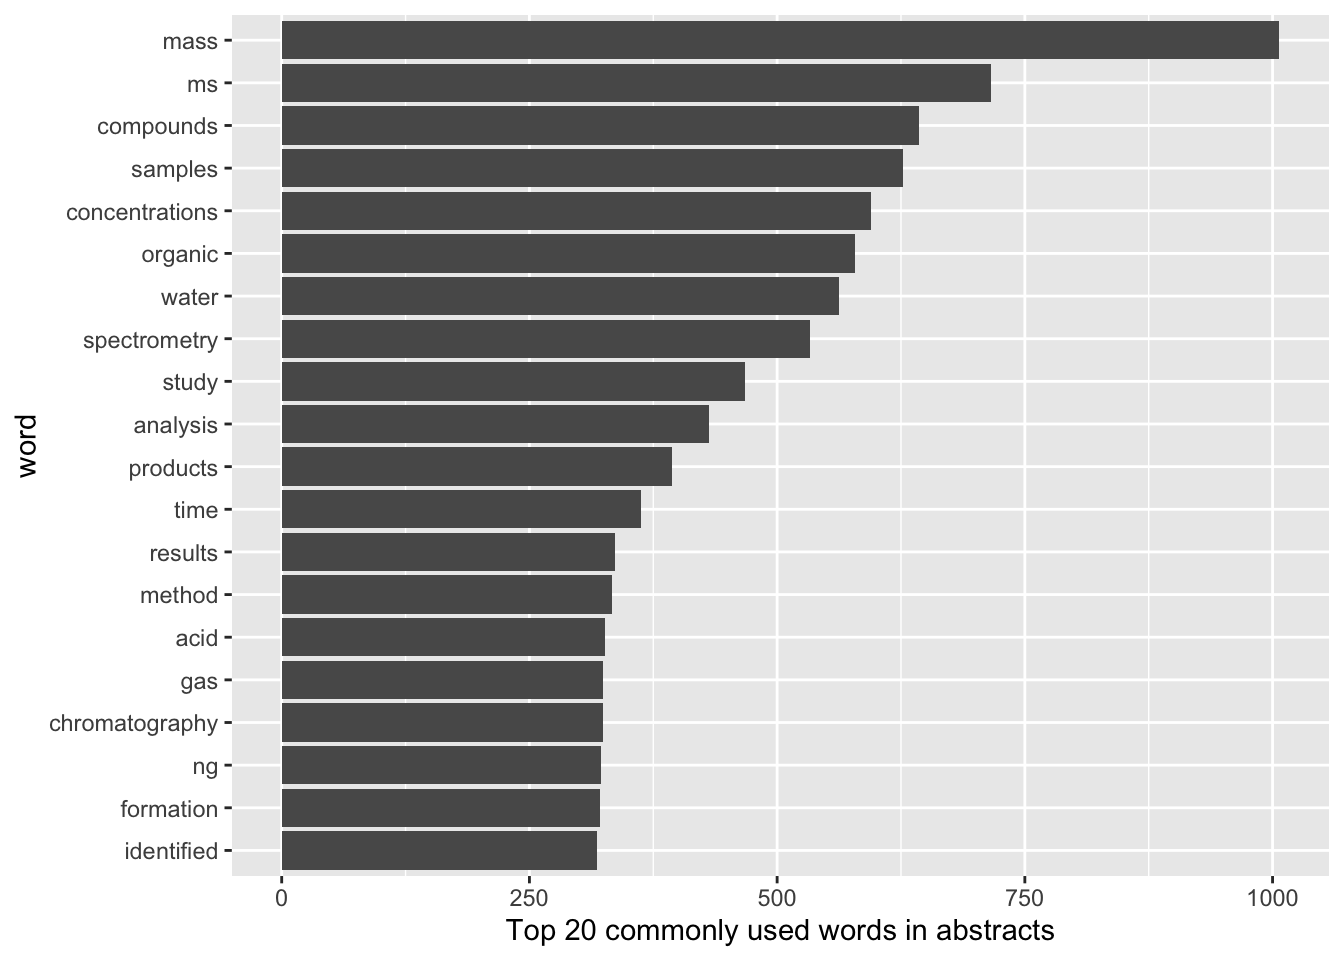
\includegraphics{sciguide_files/figure-latex/unnamed-chunk-14-1} \caption[双层高尔顿钉板对回归现象的演示,第一层产生的离散分布通过第二层钉板并未出现进一步的分散]{双层高尔顿钉板对回归现象的演示,第一层产生的离散分布通过第二层钉板并未出现进一步的分散}\label{fig:unnamed-chunk-14}
\end{figure}

另一种理解方法是:每个人的身高都有固定部分跟变动部分,固定部分是都一样的,遗传来决定,这样代际变化可以用亲代子代变动部分的不完全相关来解释。同时,达尔文的自然选择就可以构建在遗传上了,至此人口平衡与代际变异就可以有统计模型来和谐相处了,否则不论是强相关还是不相关都不能解释现实数据。回归思想可以说是统计学的中庸之道,这个将效应区分为固定跟临时两部分的思想也构成了经济学里消费函数的根基,人们消费固定部分是收入而不是短期刺激,因而政府短期加大开支并不能刺激消费,这个指导思想帮助弗里德曼拿了诺奖。

多元回归问题在多元统计方法之前都是用几何学跟数据分析来解,最多两元,高尔顿提出相关系数后,皮尔逊等人发扬光大为多元分析。

\hypertarget{ux56e0ux679c}{%
\subsection{因果}\label{ux56e0ux679c}}

因果问题很长一段时间一直是统计禁区,从学统计第一天我们就知道相关不代表因果,那么问题来了:如果相关性是个逻辑死胡同,知识如何增长?打个比方,我看到人群中某个基因的高表达与某种疾病的发病率存在相关性,怎么解释?是发病导致基因突变还是基因突变导致发病?一般到这一步就需要控制实验了,也就是说我们把控制实验当成因果关系的确认而对观测数据持谨慎态度。但这实验怎么做?找一组人,用 RNA 干扰 沉默掉他们的基因看是不是得病?现代伦理不允许。用动物模型?物种差异咋办?仿真?我们搞清楚分子层面的构建机制了吗?目前相对公认的结果来自分析流行病学,金标是队列研究、临床实验与病例对照实验。严格意义上只有临床实验最靠谱,但那就真成了拿人做实验了,治疗目的问题不大,但研究目的就存在伦理问题。自然科学里控制实验容易些,很多时候因果性不言而喻(也因为这个缺乏了统计思维)。社会科学与医学就必须解决从观察结果中发现因果性的问题,不然永远只能讨论现象,因果分析就来源于此。

其实在研究回归问题时,高尔顿曾为此迷惑不解,主要是遗传意义上讲不通,高了后还是高,但没那么高,后者暗示遗传上的因果并不完全成立。但他学生皮尔逊则很简单认为这种回归也好或相关也好就是概率的,因果关系是相关的一个特例,统计学不能也不应该讨论因果性,进而奠定了后面研究中相关不代表因果的基调,用严谨性与概率锁死了观察研究,这个表述到今天还活跃在科学研究的各个领域。

其实皮尔逊虽然从概率角度澄清了单一因素在解释现象的局限性,但他自己也发现了很多伪相关或随机相关,更麻烦的是他的学生赖特在豚鼠研究中构建了多因素路径模型来解释遗传问题。赖特在豚鼠遗传问题上假设了遗传、发育、环境与随机四种来源并用路径代数分析估计了各自影响的比重,虽然赖特自己并不认为他在用相关推导因果,但 Juder Pearl 认为这是第一次用图论来进行因果关系的探索。赖特定量算出了豚鼠子代体重增长中遗传的贡献,然而这个方法在之后的50年里被统计学界打压了。统计学家认为赖特的方法只能就事论事构建逻辑关系来进行考察,但当时的统计学主流是用``固定程序''解决问题,而大量的精力耗费在了``固定程序''的理论与细节构建。统计学家在跟别人合作时通常会让对方把数据转化为他们能处理的分布进而应用标准方法来分析,但这严重忽视了现实世界的复杂性并造成了大量统计方法的误用。现在我们知道赖特实际做的是把专业知识形成的假设因果关系进行了定量分析,而脱离专业知识的统计学正是其目前被应用导向的计算机科学超越的一个原因。在我看来,因果分析是联系统计学、专业知识与计算机科学的一个关键方法与思维工具,科研里探索的就是因果与机制,定量考察因素影响的因果分析方法是一个重要步骤。

到此我们回顾下相关,如果不能说明因果,又能说明什么?两个因素之间因果也就是一个到另一个,但相关之所以说明不了因果,其实是因为存在第三种因素或更多。但简化下三个因素之间的关系其实大概就下面这四种:

\begin{itemize}
\tightlist
\item
  A导致B,B导致C \(A\rightarrow B\rightarrow C\)
\item
  A导致B跟C \(A\rightarrow B, A\rightarrow C\)
\item
  A跟B共同导致C,控制C后A跟B相关 \(A\rightarrow C, B\rightarrow C, (C): A \rightarrow B\)
\item
  随机相关
\end{itemize}

这里我是用箭头表示因果,用括号表示控制。第一种很明显就是直接因果关系,这里因果关系是传递的,如果你控制了中间那一个,因果关系就阻断了,这是所谓的中介效应;第二种我们会观察到B与C相关,然而这种相关在控制A后会消失,A就是我们经常提到的混杂因素,例如巧克力消费量与诺奖得主数相关,背后是因为他们都跟国家经济发展水平相关,当国家经济发展水平一致时,巧克力与诺奖间的相关性就会消失。这两种接受过统计学教育的都比较容易理解,第三种就不那么直观了。

糖尿病会导致血糖高,吃糖多也会导致血糖高,正常我们是看不到糖尿病与吃糖多相关的,因为这是两回事,健康人吃糖多也会血糖高。然而,当我们控制一个高血糖浓度区间去看糖尿病发病率与吃糖行为时,他们就相关了,也就是高血糖的人既可能是病人也可能临时糖吃多了,如果我们只看一个时间点,很容易发现吃糖与糖尿病的相关。也许你会说吃糖就是导致糖尿病,但如果我们看的是I型糖尿病(遗传原因主导)呢?你也会发现相关。这种相关只在控制了血糖后出现,不控制两个没有相关性,这种相关是对撞关系在控制后导致的。很多人做研究喜欢在模型里加上尽可能多的协变量,这个方法可以处理第二种情况,但协变量如果是第三种情况控制后会把不相关的两个因素搞成相关的,这个情况很多研究人员意识不到会导致错误结论的出现。第四种情况也存在,特别是高维数据,这就是因果分析与p值问题的连接点,多重检验里如果排除随机相关或显著性已经是当前学术界意识到的问题了。

也就是说,当我们看到两个变量相关,除了因果与混杂,还存在对撞与随机相关,对撞是不恰当控制变量导致的而随机相关则对高维数据是一个灾难。因果分析所要做的就是区分这些并正确估计或探索变量间的关系,理清楚了这些基本关系,也就可以通过演绎法探索相关背后的因果了。

这里有个概念要说清楚,那就是控制。什么是控制?控制就是让某个因素恒定,在线性模型里就是加上一个变量,此时拟合后其他变量的拟合系数就是控制了这个因素后的效果。当然,如果存在非线性关系例如交互作用,控制就会复杂些。控制的神奇之处在于我们不需要事先处理而仅仅是分析时加入考虑即可。Juder Pearl 引入了 do 演算的概念来补充概率论里条件概率对控制干预的先天不足。P(A\textbar B)与P(A\textbar do(B))实际计算可能是一回事,但在因果图里就很不一样了,do 表示一种单向干预而概率论里的条件概率没有方向性。举个例子:

\(A \rightarrow B \rightarrow C, D\rightarrow A, D\rightarrow C\)

现在我们想知道A与C的关系,目前走 ABC 路径是通的,AC路径会因为存在混杂因素D也是通的,那此时你就无法认定A与C之间是否是因果关系,这个时候要做的就是对D进行控制,阻断A与C间的混杂因素途径;同时如果对B进行控制,阻断A与C之间B的中介途径。这样之后看A与C间的关系就知道剩下的因果关系了。其实更严谨的方法是 Rubin causal model(RCM),也就是 Donald Robin 提出的因果分析框架直接计算,不过用因果图更直观些。

因果图里这个过程叫做 do 分离,用 do 的控制行为隔离掉非因果影响。当我们根据推测的变量间关系画出因果图后,do 分离就可以很直观的看出来。例如面这个关系:

\(A \rightarrow B \rightarrow C \leftarrow D \rightarrow E\)

这五个变量的关系中A与E间的通路被C阻断了,所以我们什么都不用做可以直接相关判断A 跟E的因果关系。然而,如果我们对C进行控制,B与D因为对撞结构控制后相关,此时路径就通了,此时我们无法直接考察A与E的因果关系,但如果我们接着控制了B或D,路径再次被阻断就又可以讨论了。

也就是说,如果我们打算考察两个变量因果关系,首先要根据实际情况画出因果图,然后 do 分离掉所有两个变量间的路径,此时两者的相关就是因果。这个方法很直观,当变量间关系很复杂时,我们依然可以通过考察通路来找出控制方法。由于神奇的贝叶斯定律可以让你调转条件概率的方向,所以代数上你可以在一定条件下将控制过程转为条件概率,这也就实现了从观测数据里提取因果关系的目的,这套演算过程就是 do 演算,配合因果图使用非常方便。从图里手工推导 do 演算的公式对科研人员要求过高,不过现在软件已经可以代劳,你只要画出因果图,软件就可以告诉你两个变量间因果关系推导的条件概率公式,代入你的数据就可以看到结果了。

下面我们看下因果分析的案例来加深对因果分析思想的理解。先看代际遗传,高尔顿的因果图就是:

\(遗传 \rightarrow 身高\)

并且认为相关系数是1,但如果身高同时被遗传与环境决定,那么相对稳定的环境贡献了回归现象而遗传则解释了相关性。科研实验中的控制变量法或随机本质上就是对所有可能的混杂变量或中介变量进行控制来阻断考察变量间的非因果关系。然而此时我们也明白了如果控制的是对撞变量,那么实际上我们有可能打通原来不相关变量间的通路。在这里 do 的含义一定是基于因果的而不仅仅是无条件控制,这个洞见非常有价值。

我们再来看吸烟与肺癌的案例,虽然很多人都知道我们最终是通过Cornfield不等式与希尔标准来接纳的因果关系,但用因果图来理解的话其实就是 Fisher 认为存在遗传因子即导致吸烟,也导致肺癌。Cornfield 不等式的实质就是认为如果存在这个遗传因子,那么其与吸烟的相关性应该与肺癌的相关性同步增加,然而现实数据中肺癌风险在吸烟者那边高了9倍,也就是说这个基因在吸烟者那边也得高9倍。在 Fisher 单挑其他统计学家的那个年代其实没有找到这个基因,有意思的是后来真的找到了这个促进吸烟的基因,只不过对风险贡献没那么大。一个更典型的案例出现在观察数据中,研究人员发现吸烟母亲的低出生体重婴儿存活率比不吸烟母亲的要高,好像吸烟提高了低体重婴儿的出生率。这里因果图是:

\(吸烟 \rightarrow 出生体重 \rightarrow 婴儿死亡率\)

当我们控制了出生体重后,会发现吸烟降低了婴儿死亡率,这明显反常识了。这个问题其实是五年前才解决的,研究人员提出了一个先天缺陷作为出生体重与死亡率的混杂因素,此时吸烟与先天缺陷都会导致出生体重低,如果我们控制出生体重,相当于打通了这条路径:

\(吸烟 \rightarrow (出生体重) \leftarrow 先天缺陷 \rightarrow 婴儿死亡率\)

又因为先天缺陷跟婴儿死亡率相关,所以吸烟与婴儿死亡率间存在了一条控制后的非直接因果通路。具体来说,如果先天缺陷比吸烟对低体重影响更大,造成高死亡率,那么我们只看低体重婴儿的话就容易把原因归结到吸烟而不是先天缺陷之上,到此观察数据的矛盾就解决了。本质上因果图可以帮我们探索新知识,而传统统计分析则更多就事论事而导致矛盾。不过直观归直观,其实 RCM 在推导上更严谨,不过我估计外学科理解因果分析还是会收敛到因果图上,直观可视化在技术推广上总是占优。这个阶段工具很关键,哪个软件简单易用,其背后的模型就可能最终胜出。

接下来知名案例就是辛普森悖论了。当我们整体看两组数据时会有差异,然而当我们将数据分层后这个差异就会消失或逆转。具体到辛普森悖论就是一组新药对人群整体有益,然而当我们按性别区分时,这个药对男性也好女性也好都没了益处。现在比较流行的解释是基于一个数学事实:部分的比例之和与整体的比例之间没有必然联系。在辛普森悖论中,对照组病死率女性为1:19,男性为12:28,服药组女性为3:37,男性为8:12,这样我们看到 \(1:19 < 3:27\),\(12:28 < 8:12\),这样不论男性女性,对照组病死率都低于服药组,药物无效。然而我们不看性别时,整体是\(13/47>11/49\),对照组病死率比服药组高,药物又有效了。这里形成悖论的关键在于人们会理所当然认为部分比例的差异结果会传递到整体,其实 \(\frac{A}{B}<\frac{C}{D}\), \(\frac{E}{F}<\frac{G}{H}\),但\(\frac{A+E}{B+F}\)跟\(\frac{C+G}{D+H}\)间是不能传递这种关系的,数学上就不成立,所以我们的直觉给出的悖论是惯性思维的错误。

\begin{table}

\caption{\label{tab:unnamed-chunk-15}辛普森悖论}
\centering
\begin{tabular}[t]{lrrrrrrrrr}
\toprule
  & 总康复 & 总死亡 & 总病死率 & 男性康复 & 男性死亡 & 男性病死率 & 女性康复 & 女性死亡 & 女性病死率\\
\midrule
对照组 & 34 & 13 & 0.28 & 16 & 12 & 0.43 & 18 & 1 & 0.05\\
服药组 & 38 & 11 & 0.22 & 4 & 8 & 0.67 & 34 & 3 & 0.08\\
\bottomrule
\end{tabular}
\end{table}

不过这只是解释,不解决最初的问题,到底这药有用没用。这里就又牵扯到因果图了,我们得知道性别对服药与结果的影响,也就是说得知道性别的角色。首先,性别不是服药与发病结果的结果,毕竟不是变性药;其次,性别是否决定服药?经过调查发现,女性确实比男性更容易记得服药;最后,性别是不是会导致结果,调查也发现男性容易患病。好,这样分析后性别就是服药与患病的混杂因素,因此服药与患病间不形成 do 分离,我们需要控制性别。怎么控制呢?很简单,就是分开性别讨论然后按性别在人群中比例加权,最后的结果就是辛普森悖论中的新药对整体其实是有害无益的,悖论解决。我们回顾下这个过程会发现,悖论的解决实际上是依赖了因果图构建过程中外部信息的整合,单纯看数据不看背景知识的纯统计探索在这种场景下会陷入悖论。所以说因果图或因果分析其实就是引入更多的背景知识,只是当前懂专业知识的与懂统计学的还没进行很好的学科融合。

不过性别不总是共同原因,也可能是中介。这个也比想象的常见,简单说就是下面的结构:

\(A \rightarrow X \rightarrow B\)

当我们打算估计 A 到 B 的净效应时,X也作为中介在起作用。比较经典的案例就是伯克利录取问题,整体上呈现对女性的性别歧视,然而分院系看却大都是女性占优势。这个案例经常跟辛普森悖论放到一起讨论,但因果图上是不同的。辛普森悖论里性别是混杂因素,伯克利录取里,A是性别,B是录取结果,而院系则是作为中介存在的。性别不同的学生会选择不同的院系,而不同院系录取率本来也不同。通常关于这个现象的解释是女性会选择难录取的院系,这件事造成了整体与结果的不同。

不过解法上倒是类似,因为控制了 X 之后就中断了这个路径而可以直接估计 A 与 B 的关系。但控制 X 相当于得到的是这个 X 下的录取率,要想知道全局影响,还是要加权平均。传统分析里直接效应间接效应的讨论无法区别中介与混杂因素,因果图则可以很好区别出来进行解释。不过中介问题的复杂性不在这里,如果存在一个对中介与结果的混杂因素,对中介进行控制就是错的。举例来说,如果居住地会影响院系与结果,例如某个州大学的甲院系就是只录取本州男性与外州女性而乙院系则只录取本州女性与外州男性,那么我们对院系的控制实际上打开了性别与居住地的后门路径而造成了错误估计:

\(A \rightarrow X\rightarrow B, C \rightarrow X, C \rightarrow B\)

这里C代表居住地,此时我们控制 X 会导致:

\(A \rightarrow (X) \leftarrow C \rightarrow B\)

这条 A 与 B 间的因果路径打通,结果就是 A 对 B 的估计中还是存在混杂。这里我们也能看到悖论的魅力,如果条件发生改变,解决悖论的方法也要随之改变而不是简单控制就能搞定的。有时候完全不控制可能就是最好解决方案而过多的控制会让结论无法被理解,这点对机器学习里 \(y = f(x)\) 的简单逻辑框架来说是灾难性的,更多的特征值不见得拟合效果更好,反而让你说不清楚结果与变量的关系。当然,现在主流似乎也不打算说清楚。

既然说到辛普森悖论,就顺道聊下这个悖论的变体。最古老的变体是田忌赛马,为了保证整体上取胜,我们可以在部分作战采取放弃策略,这个在军事学发展中阵地战战术中比较常用,说白了就是在战力不占优的条件下通过兵力在防线上的调配来取得一定效果。这种作战方式个太古典了,现代战争的变体是海陆空高科技兵种配合作战,早就脱离了电视剧里对着砍的策略(但对着砍有戏剧性与视觉冲击力),当前作战形式基本都是地面小队配合空中扫荡与坦克掩护,你要是敢把几千人排到一个开阔阵地上等对砍搞决斗,就等着无人机包饺子吧。这很可能是互相博弈的一个结果,因为双方将领如果都明白辛普森悖论原理,那么肯定会最大化自己的优势去打对方的弱势。而现代战争是科技战,人数啥也说明不了而更多是劣势,所以不超过10人的小队突击在对战中灵活性最高且容易发挥科技领先优势。现代公司发展中,很多大公司采用传统上的多级体制其实就是在搞阵地战,技术上如果信息流通顺畅,小组制应该是整体取胜策略,我们已经看到很多互联网爆款产品最初其实都是来自小组而不是靠人数,当然后期巩固成果是完全另一类可持续策略了。在政治学里也存在辛普森悖论:杰利蝾螈。这个概念指的是通过划分选区来操纵选举结果的一种策略,通过把铁票仓分到对方的边缘选区可以在代议制选区民主里赢得多数票,民主的一人一票不代表整体不能被操纵,这对大杂居小聚居的西方移民国家尤其重要,如果争夺中间派不切实际,那就把极端分子渗透到中间派选区搞事情。

\begin{figure}
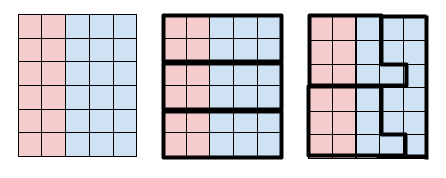
\includegraphics{data/gerrymandering} \caption[杰利蝾螈示意图(两个党派的30人分为3个10人组投票,按分组结果得两票以上获胜。如果分组按照党派在人群中的比例(中间图)则蓝党会在三个分组里都获胜,但如果控制分组(右边图)则可让红党派在两个分组里获胜,从而整体上获胜)]{杰利蝾螈示意图(两个党派的30人分为3个10人组投票,按分组结果得两票以上获胜。如果分组按照党派在人群中的比例(中间图)则蓝党会在三个分组里都获胜,但如果控制分组(右边图)则可让红党派在两个分组里获胜,从而整体上获胜)}\label{fig:unnamed-chunk-16}
\end{figure}

前面说的都是辛普森悖论的分类变量比例版,很自然,这个悖论也存在线性模型版。也就是说,一组数据做回归,变量系数是正的,但是我们把数据切成两部分,其同一变量的系数就会变成负的。这个线性版的成因除了跟前面比例版一样外还存在另一个成因,那就是噪声。当参与回归的变量只能解释数据变异中一小部分时,其回归估计参数的不确定性会被未知变异所主导,如果分割数据的方法与未知变异混杂,那么变量的方向就会不稳定。这里还是要强调下参数估计一定要包含不确定性,如果不确定性高不代表结果不靠谱而更可能是数据结构还没搞清楚或数据量不够。其实这种信噪比不够的问题与前一章所述的可重复性危机有关,也许我们花大力气估计清楚了一个微弱变量的效益,这是否值得?学术上当然值但现实意义就不好说了。

除了我上面提到的,经济生活中也有辛普森悖论,例如股票指数走高里不代表每个板块都高,这就联系到风险控制与对冲了。辛普森悖论告诉我们存在整体收益而部分损失的可能与部分都受益但整体依旧损失,整体与部分数学上其实没关系,数据上就要看背景了,最好用因果分析来探索下究竟是什么导致的差异及加权后整体究竟怎样,当然,如何加权,用什么加权,逻辑通不通其实有时是艺术而不是科学:你把因果箭头反着来能说通也会产生一个估计,自圆其说不解决科学求真的问题。

前面我一直在说加权,感觉好像搞清楚因果关系后剩下的就是加权平均的计算,其实实际也是这样。因果分析还有种做法就是通过计算个体因果效应后计算整体平均因果效应(ACE)来做的,这个平均过程也可看出某种加权,就是做了跟不做后的净效应。不过这仅仅是计算层面,不包含因果假设。

\[ACE = E[Y{i,1}] −E[Y{i,0}]\]

因果图另一个应用是工具变量。当然工具变量在计量经济与公共卫生领域里有不同的表述,但本质上就是如果我观察 \(A \rightarrow B\) 时存在 C 同时影响 A 与 B,那我们就找一个不受 C 的变量 X,这个变量直接作用于 A,此时我们计算 A 与 X 的相关性与 B 与 X 的相关性,根据下面的因果图:

\(X \rightarrow A \rightarrow B, C \rightarrow A, C \rightarrow B\)

X 与 B 之间没有直接因果,在效应计算中,X 与 B 的相关只会来自于 A 的中介,也就是 A 与 X 的相关性与 A 与 B 的相关性乘积,如果我们打算估计 A 与 B 因果效应,就是用 B 与 X 的回归系数去除 A 与 X 的回归系数。这个过程中因为 C 跟 X 间没有因果通路,所以相当于跳过了混杂因素的讨论。这个路径影响等于回归系数乘积的代数技巧使得计算上非常清晰,但还是牢记工具变量的选择不是探索的而是因果的,需要背景知识。有了工具变量,研究人员就从无穷的相关与混杂中解放出来而可以通过因果图构建来求解目标因果关系。当因果图很复杂时,你需要去控制一些变量或引入工具变量实现你关心变量的 do 分离,进而估计净效应。

因果图天然与贝叶斯分析有联系,且不论条件概率的转化,因果图跟贝叶斯网络就存在内生联系。构建因果图需要的背景知识可以类比成贝叶斯预设的网络层级,因此在求解上类似。复杂因果图实际也常常跟结构方程模型放在一起讨论,因为这两个解决的问题基本就是一回事,不过结构方程模型里并不存在控制而更多侧重参数求解,因果图除了可以玩控制变量 do 分离外,也可以接纳非线性关系。在有明确定义的结构因果模型(也就是复杂因果图)里,可解释性被放在了第一位,也就是说数据驱动的假设被模型驱动所取代,这放在机器学习领域里看起来像是开倒车了。不过因果图很难直观表示交互作用而更多用在线性模型里,所以看起来结构方程模型似乎是目前因果图用的最多的地方。

在统计学家 Juder Pearl 看来,当前的机器学习也好,人工智能也好,都卡在了因果分析的第一层,也就是关联这一层,到处都是相关且多数人似乎放弃了模型的解释性而一味追求预测与关联。他进而提出了因果关系的第二层(干预层)与第三层(反事实层)。其实这有点类似科学哲学的发展,第一层类似归纳分析与观察的实证主义,第二层则可以对应实验主义,第三层则是则类似证伪的思路,进而构想出一个不同于现实世界的客观知识的世界(波普的世界三)。不同于主流对模型可解释性的放弃,因果分析从一开始就构建在因果关系之中,解释起来相对容易(自然要因果图加持),不同数据间存在自己的数据逻辑结构,高层级的算法要能通过干预与反事实假设来发现结构,只有这样的算法才能实现强人工智能,因为人的思考就是因果的。 Juder Pearl 的哲学观里因果不是相关的特例而是反过来,相关里浸润着不同的因果,因果分析就是对这些东西的关系加以区分。

这个观点确实像是开倒车,用决定论反击概率论,但也可能是一次对当前科研的矫正。太多研究人员在大数据浪潮下放弃了可解释性而追求预测精度,且因为算力的加强,原来很多理论求解几乎全变成了数值求解。同时深度学习等神经网络的应用也让解释模型越来越变成一个笑话,不过如果我们真的不研究认识问题,那人类是否还能发现新理论与新机制?从来都没有单纯的数据驱动的研究,所有的数据驱动背后都有对问题的建模,当模型假设错了以后,数据再多也是缘木求鱼。不过是不是物理或化学模型就没问题了?也不是,理化生的知识大都是构建在还原论上的,理论会被设定在理想环境之下,这也对现实脱了节。自下而上与自上而下不存在哪个是真理的问题而仅仅就是个历史问题,因果分析可能是相互连接的一个工具。不过目前因果分析更多是应用在偏软科学与数据优先的学科里,理论优先的学科从一开始就是在讨论因果,但因为使用的是统计工具,所以内在的相关不能定因果的观念事实上是被学科自己的理论给压制了,但这也造成了对统计工具的滥用与误用。

长远看因果革命可能在两方面实现突破:一是统计学家对实际问题背景知识的接纳与考量而不是研究纯理论细节;另一方面是科学家对统计工具的重新理解,从因果图角度探索自己科学问题的解决方案。但无论如何,因果分析的思想都是很有前景的,因为这个工具是为思考服务的,现代人囿于工具人角色,缺的就是这一块。

\hypertarget{ux6b8bux5dee}{%
\subsection{残差}\label{ux6b8bux5dee}}

残差本质上科学就是通过解释剩余现象进步,而当今其实理论体系里留给重大发现的空间是有限的,所有人都在精进1\%,不过都是在80\%-90\%的基础上的,也就是大家伙都在噪声里探索信号的模式。具体到统计模型就是对模型解释不了的部分与模型诊断的思想,有了这个思想统计学就有了不断发展的动力与自我审视的原则。从科学角度看,残差思想更重要的提示在于去思考实验设计或假设检验之外的东西,除了你关注的点也要留心那些被你控制随机化之后依然存在规律性的东西,否则科学就只有验证的功能而丧失了探索的可能。

\hypertarget{ux6a21ux578bux601dux7ef4}{%
\section{模型思维}\label{ux6a21ux578bux601dux7ef4}}

模型思维是一种一对多的思维方法,从相似的事实中提炼出逻辑规律,用规律来指导认知世界,这种思维的优势在于逻辑或者说理性起决策主导参考作用。当一个模型出错时,我们可以运用其他模型来研究某个事实,因为所有的模型都存在简化,所以知道模型越多越有利于理解世界里发生的事。模型都有自己的准确度与适用范围,一般而言,高准确度的模型适用范围比较精确且会形式化为公式,而低准确度模型类似万金油,无所不包但含义模糊。模型化思考是首先抽离出变量,然后确定变量间关系,最后运用逻辑推理来进行思考的过程,这对于科学探索非常重要。模型或规律的终点可能是循环的、平衡的、随机的与不确定的,要用学会概率角度而不是决定论去描述结果。

模型主要有两种,一种是基于公式的,另一种则是基于单元进行模块组合的仿真模型,前者需要你清楚的了解模型机理,后者则需要假定单元的活动空间与行为方式,然后通过模型运转来了解整体变化。下面首先讨论让模型思维可以落地的可编程思维,然后讨论个体常用的决策模型,之后是个体与整体关系及动力学模型,最后研究下常见的真实问题求解模型。这些模型思维对于科研是很重要的工具,这方面书可参考斯科特·佩奇的《模型思维》。

\hypertarget{ux7f16ux7a0b}{%
\subsection{编程}\label{ux7f16ux7a0b}}

编程是计算机科学的核心概念,当一件事可编程时,我们就可以设计出相对的硬件与软件来自动化这个过程,这个是模型思维在可执行角度的重要体现。对于科研人员,硬件方面一般较少涉及,软件编程却是日趋日常化。因此,我们有必要了解编程语言的一些基本概念与思想。

程序是编程的结果,一般包含一条或一组执行运算的指令,这里运算并不仅仅指数学运算,也包括所有可通过电子电路完成的运算。要实现一次运算,我们至少需要输入值、运算与输出值。运算至少要能实现数值运算、顺序执行、条件执行与循环。因此,如果你打算进行编程,你就需要通过计算机语言让计算机知道输入输出与运算过程。

计算机语言不同于日常交流的自然语言(虽然可以处理自然语言),其核心特质在于描述上的准确性。不论操作符、数据类型还是函数定义,不同的计算机语言都有自己的规范来确保人要求的抽象化与机器能听懂人的要求之间达到平衡。底层语言例如汇编语言机器非常容易懂,但人不容易将需求转化为汇编语言。高级语言需要编译成底层语言来执行,不过人相对容易将需求进行编程。这个编译过程会损失效率,所以一般学习的语言越容易,效率与准确性往往会受影响。

科研里一般用程序来处理数据,所以科研编程的语言选择往往是实现效率、处理方法与编程难度的平衡。一般来说,数据处理方法源于统计学知识,编程难度取决于学科现实问题的抽象模型而实现效率属于纯计算机科学问题,科研人员可根据自己知识背景进行选择。对于非计算机科学专业的科研人员,建议关注学科内主流编程语言,否则后期会有很多交流上的困难,或者一步到位实现程序的应用化,让用户在少量编程知识的背景下就可以应用。

学习编程语言一般首先要掌握变量类型、赋值、表达式语法、保留词、注释等基本概念,然后就是大量的交互式案例训练来熟悉用法。编程语言一般会自带 REPL (Read--Eval--Print Loop;读取-执行-打印循环) 程序,在这个程序下会识别该编程语言的语法与操作符,互动地输入输出数据与结果。在编写程序代码时,最基础的要求是搞清楚编程语言的优先级,例如括号\textgreater 指数\textgreater 乘除法\textgreater 加减法,一般执行顺序是从左到右。

另一种使用编程语言的方式是通过独立程序实现特定功能来完成的,运行程序可以直接得到输出,人机互动是在应用层上的。 REPL 方式其实比较符合数据分析的需求,后一种方式则反映了软件工程,涉及了程序的设计、构架与封装。目前科研应用中侧重交互式数据分析而业界则更看重程序编写与功能实现,前者存在试错且探索为主,后者则更侧重目标。这个区别专业程序员或软件工程师经常体会不到,觉得用 REPL 的科研数据分析是初学者,不能算编程。但其实科研数据分析的核心就是计算与需求的互动,REPL 只是其中一种,将需求从 REPL 用户过度成函数程序也是很重要。

也就是说,交互式与独立程序之间往往还有一个中间态,可以是脚本,也可以是自定义函数。一段代码一般是以输入为始,以输出为终,中间有函数来处理数据。在固定模式的数据处理中,一个函数的输出往往可以是另一个函数的输入,将输入输出代码按顺序、条件、循环排好就可以产生一个新的组合函数。事实上很多高级语言就在逻辑上抽象出一些常用函数来方便程序员直接调用。

同时,为了实现具体的功能,函数的输入除了数据外还有一些参数,有些是经验值,有些则可能要来自于功能本身定义。在输出上,有些函数的输出可以返回数值,有的可能就是打印到屏幕上就结束了,根据实际需求来。此外,多数语言的函数内部变量是只在内部可生产或可调用的,内部没有就可能从当前环境里找,最好不要设计这样的程序。函数或脚本对数据分析最大的意义在于减少重复工作与理清分析思路,对于软件工程则属于搭建工程部件,无论如何都是件功在当代利在千秋的事。

如果程序设计有问题,编程语言也会有对应 debug 的过程,大多数情况下是编程者的需求与机器的执行不对应导致,可以从这里入手思考修改代码。常见的错误包括但不限于语法错误、语义错误与例外。

下面重点讨论下编程思维中一些常见现象与术语,侧重理解并最好通过联系来强化理解。

\begin{itemize}
\item
  条件分支:函数中出现需要对数据子分类进行不同运算时的设计,不同子分类用不同条件语句进行逻辑判断,例如数值求绝对值要先判断正负。
\item
  循环:同样的操作要对不同的可索引或满足特定条件的数据进行运算,这种情况要设计循环结构,例如按数据行/列求值。有些循环循环数是知道的,有些则要对数据运行结果进行判断,满足特定条件时可跳出或继续循环。
\item
  递归:比较特殊的条件与循环结构,当数据不满足某条件时就执行函数本身直到满足条件,例如求解斐波那契数列之和就可以设计递归结构循环执行本身直到数据可计算的起点。递归的效率一般不高,但递归结构有助于简化思考问题的步骤。
\item
  正则表达式:正则表达式是字符串处理时常用的模式识别工具,灵活使用正则表达式与条件分支可以有效处理真实数据中的混杂,强烈推荐\href{https://zh.wikipedia.org/zh-hans/\%E6\%AD\%A3\%E5\%88\%99\%E8\%A1\%A8\%E8\%BE\%BE\%E5\%BC\%8F}{学习}掌握。
\item
  数据结构:通常不同数据按照实际需求会有不同的格式,不同格式的数据处理方式会不一样,一般函数都会先验证数据结构,如果不能处理则返回错误。
\item
  数据表:常见的数据处理格式,一般不同行表示不同样品,不同列表示不同样品属性且数据类型一致,数据值可以是数值、字符或逻辑值但不能是数据表。由于数据处理算法大都基于数据表开发,这类格式数据比较容易找到现成的算法函数/库/扩展包来进行处理。
\item
  字典:很多程序语言支持字典,字典是一种对应关系,字典中的元素是键值-数值对,通过键值索引数值,也可以反查。数据表中搜索元素是按照数值索引顺序索引的,字典则可以用哈希表快速索引。字典可以在编程中用来构建基于输入的数据库,方便进一步查询。
\item
  列表:列表属于数据表与字典的泛化,列表元素可以是数据表或列表,因此列表的数据结构不是平行的而是具备层级,有的元素可以进一步展开。列表常用来表示一组关联概念且可以数值索引,例如在回归分析的返回值中,就会包括拟合值、回归系数、残差等数据表或数值。
\item
  类型:通常列表可被定义成一种新通用类型,算法可基于这个类型进行开发或泛化,例如当你调用画图程序时,其程序会首先判断你输入数据的类型,如果有对应方法则直接调用,没有则用通用方法或返回错误。有些语言中列表是不能直接操作的,这样设计就是为了防止类型不兼容而强制定义格式。
\end{itemize}

此外,应该了解一点C语言,因为C语言是多数操作系统的基础,所以多数操作系统也自带对应的C编译器。更重要的是,C语言的库很丰富,也就是工具函数比较多,换别的就得自己写。这是很有意思的路径依赖案例,事实上任何语言都应该可以拿来写操作系统,不过C是在开发Unix时候设计出来的,现在流行的开发级操作系统都是unix/类unix操作系统,加上C在内存管理与CPU交互上的先天优势,历史机遇下成为了主流。C语言源码编译运行过程是这样的:先预处理源码,调入模块,然后转换成汇编语言文件,汇编语言文件可以被汇编器转为机器码,然后通过连接器合并为可执行文件,最后加载到内存里运行。

C的核心地位还体现在很多高级语言的编译器是构建在C之上的,或者是C++之上,多数高级语言都通过限制自由度(例如不让操作内存、功能模块化等)来实现上手容易与较高的开发效率,但只要关注程序性能,肯定回去学C或C++的。GNU的GCC编译器是一个相对通用的编译器合集,可以用来编译包括C在内的多种语言。然而,GCC也是有历史包袱的,所有有人就另起炉灶单独针对C或C++重写了效率更高的编译器及其后台,这就是苹果的LLVM项目与clang编译器。但要注意的是LLVM支持的语言不如GCC多,所以如果你还要用到fortain或java编译器,那就还是老老实实用GCC吧,或者cmake的时候分别指定编译器,只要你不嫌麻烦。一般而言,效率与性能往往不能兼得。

高级语言的编译过程跟相对底层的C或C++是不一样的,Java就是自己定义了一套运行环境JVM,编译出的文件也是JVM可读的,这就提高了Java的可移植性,降低了跨平台开发的难度,当然你得保证这些平台上可以运行JVM。其实很多高级语言是解释型的,REPL里可直接运行代码,但同样会有人为高级语言写编译器来提高运行性能,这个是按需求来。我个人感觉是用REPL的人一般是应用层的,关心有没有满足自己需求的函数;用编译语言的人一般是开发层的,关心软件工程及性能。然而,高级语言里如果打算提高运行效率,也会提供C或C++的接口让程序员可以通过外力来提高自由度。过度的功能封装实际也限制了高级语言的应用场景。

说到效率,自然少不了并行计算,openmp 就是一种并行化方案,可以支撑C与C++。很多R包会通过使用 openmp 来底层加速算法,但这样的包一般都需要单独编译。目前GCC与Clang在编译器层其实都实现了对 openmp 的支持,编译时加上 -fopenmp 就可以。

其他一些概念例如云计算、单元测试、集成测试、GPU加速、功能模块化、环境容器化、接口调用、功能移植、数据库检索、前端设计、数据加密、移动端兼容等都很有了解的必要,但这是建立在牢靠的基础上的。一个简单的判断标准就是根据你的需求你会觉得存在某种设计,然后一搜索发现果然有这样的领域,从需求出发回到需求中去是编程思维的要诀,不要在屠龙之术上花费太多时间。

\hypertarget{ux51b3ux7b56ux6a21ux578b}{%
\subsection{决策模型}\label{ux51b3ux7b56ux6a21ux578b}}

个体行为都是有自己决策过程的,决策模型分为多准则决策与概率决策,前者可以定性分析,也可以打分定量分析,可以使用空间量表可视化多维选择。概率决策是构建在事件及其后续事件发生可能性基础上的,赋值后根据决策树反推不同选择下的期望结果。基于概率决策树可以对信息定价,推算在有无信息下的期望差就是信息的价值。

人的思维过程跟物理世界运行规则是不一样的,有的人喜欢严格按规则办事的,有的人则看心情办事,还有理性行动者。按规则办事的人可以靠规则来预测,例如博弈论里的分析与随机选择,决策越简单越容易执行。看心情决策的跟随机过程差不多,永远不要尝试预测一个随机事件。理性行动者会不断按目标函数寻优,经济学里的理性人假设就是如此,但存在边际效用递减的情况,也就是前期改善大后期改善不明显的情况。理性不意味自私,跟个人目标或价值认同符合的决策有时需要考虑群体最优。真实世界的人三种思维模式都存在,不同场合不同组合。很多时候基于规则的经验可能是最符合现状的,既不会绝对理性,也不会过于随意,大概取个中间值,为不确定性留空间。

规则模型里比较常见的是分类模型与线性模型。分类模型就是把相似的东西归到一类里去,分类越能捕捉群体里的差异,模型就会越符合现实,其实就是组内方差最小化与组间方差最大化的体现。线性模型则是通过构建拟合两个变量的线性关系来进行预测,线性模型中,R方可以用来描述模型解释度,系数正负可以告诉你效应方向,系数的量级可以表现系数的重要程度,系数的p值可以告诉你出错的概率。现实数据可以拆分成不同线性阶段,这样非线性就可以线性考察。重要系数的筛选属于循证研究,首先构建模型,然后收集数据,然后确定重要变量,然后改变变量来看影响,进而找出影响大的变量。线性模型也存在局限,例如不能识别因果,对于反馈作用无法预测,例如早先设计ABS系统是因为车距过近容易出事故,但有了ABS后实际车距反而缩小了,因为人们把ABS的影响反馈到行为里去了。

除了线性模型外,非线性模型可以看成线性模型的组合,这样就会存在临界点,不过要区分指数模型与临界点模型,他们内在动因不同,临界点前后量化属性会发生变化。在传染病模型中,临界点就是基本传染数。临界点可以通过多样性指数或熵来测量:多样性指数就是不同类型概率平方和的倒数,越高多样性越高;熵则是概率与概率对数的乘积和的负数(信息可加和并考虑概率),越高越混乱,需要信息越多。

\hypertarget{ux4e2aux4f53-ux6574ux4f53ux6a21ux578b}{%
\subsection{个体-整体模型}\label{ux4e2aux4f53-ux6574ux4f53ux6a21ux578b}}

当人聚到一起后,整体就会有自己的属性,系统的表现取决于环境、个体间关系与系统组织结构,与个体属性关系就不大了。单一行为的聚合模型可以考虑中心极限定理;单一规则的聚合模型可以参考细胞自动机的研究,此时已经有系统高层次动态了;个体的偏好聚合后就会出现系统高层次矛盾,例如博弈论、投票、群体非理性等。

在整体个体决策价值判断分为两种,一种是无个体最优的价值属性,例如颜色偏好,一种是越多越好或越少越好的个体与群体取向一致的属性,例如幸福度、效率质量。前者相关模型多用于政治学,例如中间选民理论里持温和派观点的候选人往往能得到多数票,但这只在单一维度上成立,也就是为了意识形态而放弃理性时会成立,当多维度出现时,中间选民需满足径向对称(radial symmetry)才胜出,否则就是无胜出结果(Plott's no-winner result),任何可能都会出现。现实世界中,单一维度模型往往能解释大多数情况,但政客也经常通过反复无常来应对民意的波动。在单一维度模型时,提议者要尽量争取中间派,而中间派关注自己立场与现状与新政的距离,只有新政距离中间派距离小于现状与中间派距离才能争取到。同理,现状越极端,新政越有可能通过,这是现状与中间派权力间的博弈。多层级政府里法案的通过需要多方认可,这种有利于权力制衡,但阻碍效率(Voronoi 图可用来可视化选择域)。个体与群体取向一致的属性上,可采用上述决策模型,但现实世界中通常混杂个人偏好与群体取向。在一个市场里,如果竞争充分,客户价格敏感度往往比较高,如果竞争不充分,调价空间就很大,非实用品质因素例如品牌等个人偏好的因素往往主导目标人群的决策。就具体商品而言,个体选择(无最优)、社会功用(最优)与资源稀缺性(现状)都是定价要考虑的,单独考虑一个会产生系统偏见。

社会有时为了整体利益会奖励个体的行为,荣誉、品牌、学历等社会信号就是这类机制。这些信号可能对个体生存没有意义,但可以塑造社会地位。无私的捐赠、浪费式消费与精美的手工艺品都属于这类信号,奢侈品的营销策略就如此,通过营造氛围让普通商品玩不起这个游戏,也就是有钱不如有闲。我们可以利用社会信号这一非生存需求设计规则来募捐或促进社会公益事业发展,各取所需而不是简单嘲讽或批判。个体的进步可以来自自我认同,也可以来自社会认同,一个纯自我认同的个体很可能对社会公益毫无兴趣,此时要设计机制让其了解社会认同的优点,内部激励靠钱带来的个人欲望,外部激励靠名带来的模仿效应。

个体行为在群体中有两种形态,一种是同群效应,也就是被群体同化,细分也有两种,一种是直接服从整体,另一种是在周围环境压力达到自己设定时被同化,例如起立鼓掌模型;另一种则是物以类聚,也就是只跟自己相似的人聚集,如果被群体排斥就离开,例如谢林模型,这里微观的动机不同于宏观的表现。这两种状态宏观上都会造成隔离,但形成原因差异很大,一个是入乡随俗,另一个是回归舒适区。存在引导群体行为的策略,入乡随俗的可以加强引导而回归舒适区的可以强调区别,传销的人两种方法是交替使用的。在一个群体中,个人阈值的分布很重要,如果阈值多样性大且是正反馈的,那就容易出现爆炸或崩溃,然而,当是负反馈时,个体多样性阈值会让系统趋于平衡或循环,两者都有就会是复杂的。谢林的《微观动机与宏观行为》值得作为这个问题的参考。

\begin{Shaded}
\begin{Highlighting}[]
\CommentTok{\# 谢林隔离模型,代码源于 https://simulatingcomplexity.wordpress.com/2016/01/06/building{-}a{-}schelling{-}segregation{-}model{-}in{-}r/}
\CommentTok{\# 生成单元格矩阵,两种颜色随机分布}
\NormalTok{number}\OtherTok{\textless{}{-}}\DecValTok{2000}
\NormalTok{group}\OtherTok{\textless{}{-}}\FunctionTok{c}\NormalTok{(}\FunctionTok{rep}\NormalTok{(}\DecValTok{0}\NormalTok{,(}\DecValTok{51}\SpecialCharTok{*}\DecValTok{51}\NormalTok{)}\SpecialCharTok{{-}}\NormalTok{number),}\FunctionTok{rep}\NormalTok{(}\DecValTok{1}\NormalTok{,number}\SpecialCharTok{/}\DecValTok{2}\NormalTok{),}\FunctionTok{rep}\NormalTok{(}\DecValTok{2}\NormalTok{,number}\SpecialCharTok{/}\DecValTok{2}\NormalTok{))}
\NormalTok{grid}\OtherTok{\textless{}{-}}\FunctionTok{matrix}\NormalTok{(}\FunctionTok{sample}\NormalTok{(group,}\DecValTok{2601}\NormalTok{,}\AttributeTok{replace=}\NormalTok{F), }\AttributeTok{ncol=}\DecValTok{51}\NormalTok{)}
\CommentTok{\# 找邻居函数}
\NormalTok{get\_neighbors}\OtherTok{\textless{}{-}}\ControlFlowTok{function}\NormalTok{(coords) \{}
\NormalTok{        n}\OtherTok{\textless{}{-}}\FunctionTok{c}\NormalTok{()}
        \ControlFlowTok{for}\NormalTok{ (i }\ControlFlowTok{in} \FunctionTok{c}\NormalTok{(}\DecValTok{1}\SpecialCharTok{:}\DecValTok{8}\NormalTok{)) \{}
                
                \ControlFlowTok{if}\NormalTok{ (i }\SpecialCharTok{==} \DecValTok{1}\NormalTok{) \{}
\NormalTok{                        x}\OtherTok{\textless{}{-}}\NormalTok{coords[}\DecValTok{1}\NormalTok{] }\SpecialCharTok{+} \DecValTok{1}
\NormalTok{                        y}\OtherTok{\textless{}{-}}\NormalTok{coords[}\DecValTok{2}\NormalTok{]}
\NormalTok{                \}}
                
                \ControlFlowTok{if}\NormalTok{ (i }\SpecialCharTok{==} \DecValTok{2}\NormalTok{) \{}
\NormalTok{                        x}\OtherTok{\textless{}{-}}\NormalTok{coords[}\DecValTok{1}\NormalTok{] }\SpecialCharTok{+} \DecValTok{1}
\NormalTok{                        y}\OtherTok{\textless{}{-}}\NormalTok{coords[}\DecValTok{2}\NormalTok{] }\SpecialCharTok{+} \DecValTok{1}
\NormalTok{                \}}
                
                \ControlFlowTok{if}\NormalTok{ (i }\SpecialCharTok{==} \DecValTok{3}\NormalTok{) \{}
\NormalTok{                        x}\OtherTok{\textless{}{-}}\NormalTok{coords[}\DecValTok{1}\NormalTok{]}
\NormalTok{                        y}\OtherTok{\textless{}{-}}\NormalTok{coords[}\DecValTok{2}\NormalTok{] }\SpecialCharTok{+} \DecValTok{1}
\NormalTok{                \}}
                
                \ControlFlowTok{if}\NormalTok{ (i }\SpecialCharTok{==} \DecValTok{4}\NormalTok{) \{}
\NormalTok{                        x}\OtherTok{\textless{}{-}}\NormalTok{coords[}\DecValTok{1}\NormalTok{] }\SpecialCharTok{{-}} \DecValTok{1}
\NormalTok{                        y}\OtherTok{\textless{}{-}}\NormalTok{coords[}\DecValTok{2}\NormalTok{] }\SpecialCharTok{+} \DecValTok{1}
\NormalTok{                \}}
                
                \ControlFlowTok{if}\NormalTok{ (i }\SpecialCharTok{==} \DecValTok{5}\NormalTok{) \{}
\NormalTok{                        x}\OtherTok{\textless{}{-}}\NormalTok{coords[}\DecValTok{1}\NormalTok{] }\SpecialCharTok{{-}} \DecValTok{1}
\NormalTok{                        y}\OtherTok{\textless{}{-}}\NormalTok{coords[}\DecValTok{2}\NormalTok{]}
\NormalTok{                \}}
                
                \ControlFlowTok{if}\NormalTok{ (i }\SpecialCharTok{==} \DecValTok{6}\NormalTok{) \{}
\NormalTok{                        x}\OtherTok{\textless{}{-}}\NormalTok{coords[}\DecValTok{1}\NormalTok{] }\SpecialCharTok{{-}} \DecValTok{1}
\NormalTok{                        y}\OtherTok{\textless{}{-}}\NormalTok{coords[}\DecValTok{2}\NormalTok{] }\SpecialCharTok{{-}} \DecValTok{1}
\NormalTok{                \}}
                
                \ControlFlowTok{if}\NormalTok{ (i }\SpecialCharTok{==} \DecValTok{7}\NormalTok{) \{}
\NormalTok{                        x}\OtherTok{\textless{}{-}}\NormalTok{coords[}\DecValTok{1}\NormalTok{]}
\NormalTok{                        y}\OtherTok{\textless{}{-}}\NormalTok{coords[}\DecValTok{2}\NormalTok{] }\SpecialCharTok{{-}} \DecValTok{1}
\NormalTok{                \}}
                
                \ControlFlowTok{if}\NormalTok{ (i }\SpecialCharTok{==} \DecValTok{8}\NormalTok{) \{}
\NormalTok{                        x}\OtherTok{\textless{}{-}}\NormalTok{coords[}\DecValTok{1}\NormalTok{] }\SpecialCharTok{+} \DecValTok{1}
\NormalTok{                        y}\OtherTok{\textless{}{-}}\NormalTok{coords[}\DecValTok{2}\NormalTok{] }\SpecialCharTok{{-}} \DecValTok{1}
\NormalTok{                \}}
                
                \ControlFlowTok{if}\NormalTok{ (x }\SpecialCharTok{\textless{}} \DecValTok{1}\NormalTok{) \{}
\NormalTok{                        x}\OtherTok{\textless{}{-}}\DecValTok{51}
\NormalTok{                \}}
                \ControlFlowTok{if}\NormalTok{ (x }\SpecialCharTok{\textgreater{}} \DecValTok{51}\NormalTok{) \{}
\NormalTok{                        x}\OtherTok{\textless{}{-}}\DecValTok{1}
\NormalTok{                \}}
                \ControlFlowTok{if}\NormalTok{ (y }\SpecialCharTok{\textless{}} \DecValTok{1}\NormalTok{) \{}
\NormalTok{                        y}\OtherTok{\textless{}{-}}\DecValTok{51}
\NormalTok{                \}}
                \ControlFlowTok{if}\NormalTok{ (y }\SpecialCharTok{\textgreater{}} \DecValTok{51}\NormalTok{) \{}
\NormalTok{                        y}\OtherTok{\textless{}{-}}\DecValTok{1}
\NormalTok{                \}}
\NormalTok{                n}\OtherTok{\textless{}{-}}\FunctionTok{rbind}\NormalTok{(n,}\FunctionTok{c}\NormalTok{(x,y))}
\NormalTok{        \}}
\NormalTok{        n}
\NormalTok{\}}
\FunctionTok{par}\NormalTok{(}\AttributeTok{mfrow=}\FunctionTok{c}\NormalTok{(}\DecValTok{1}\NormalTok{,}\DecValTok{2}\NormalTok{))}
\FunctionTok{image}\NormalTok{(grid,}\AttributeTok{col=}\FunctionTok{c}\NormalTok{(}\StringTok{"black"}\NormalTok{,}\StringTok{"blue"}\NormalTok{,}\StringTok{"yellow"}\NormalTok{),}\AttributeTok{axes=}\NormalTok{F)}
\CommentTok{\# 设定喜好度,此处设定为50\%,也就是单元格里人周围少于四个单元格的人与自己颜色相同时,这个人就会随机搬家到另一个单元格}
\NormalTok{alike\_preference}\OtherTok{\textless{}{-}}\FloatTok{0.5}
\CommentTok{\# 模拟搬家十次}
\ControlFlowTok{for}\NormalTok{ (t }\ControlFlowTok{in} \FunctionTok{c}\NormalTok{(}\DecValTok{1}\SpecialCharTok{:}\DecValTok{10}\NormalTok{))\{}
\NormalTok{        happy\_cells}\OtherTok{\textless{}{-}}\FunctionTok{c}\NormalTok{()}
\NormalTok{        unhappy\_cells}\OtherTok{\textless{}{-}}\FunctionTok{c}\NormalTok{()}
        \ControlFlowTok{for}\NormalTok{ (j }\ControlFlowTok{in} \FunctionTok{c}\NormalTok{(}\DecValTok{1}\SpecialCharTok{:}\DecValTok{51}\NormalTok{)) \{}
                \ControlFlowTok{for}\NormalTok{ (k }\ControlFlowTok{in} \FunctionTok{c}\NormalTok{(}\DecValTok{1}\SpecialCharTok{:}\DecValTok{51}\NormalTok{)) \{}
\NormalTok{                        current}\OtherTok{\textless{}{-}}\FunctionTok{c}\NormalTok{(j,k)}
\NormalTok{                        value}\OtherTok{\textless{}{-}}\NormalTok{grid[j,k] }
                        \ControlFlowTok{if}\NormalTok{ (value }\SpecialCharTok{\textgreater{}} \DecValTok{0}\NormalTok{) \{}
\NormalTok{                                like\_neighbors}\OtherTok{\textless{}{-}}\DecValTok{0}
\NormalTok{                                all\_neighbors}\OtherTok{\textless{}{-}}\DecValTok{0}
\NormalTok{                                neighbors}\OtherTok{\textless{}{-}}\FunctionTok{get\_neighbors}\NormalTok{(current)}
                                \ControlFlowTok{for}\NormalTok{ (i }\ControlFlowTok{in} \FunctionTok{c}\NormalTok{(}\DecValTok{1}\SpecialCharTok{:}\FunctionTok{nrow}\NormalTok{(neighbors)))\{}
\NormalTok{                                        x}\OtherTok{\textless{}{-}}\NormalTok{neighbors[i,}\DecValTok{1}\NormalTok{]}
\NormalTok{                                        y}\OtherTok{\textless{}{-}}\NormalTok{neighbors[i,}\DecValTok{2}\NormalTok{]}
                                        \ControlFlowTok{if}\NormalTok{ (grid[x,y] }\SpecialCharTok{\textgreater{}} \DecValTok{0}\NormalTok{) \{}
\NormalTok{                                                all\_neighbors}\OtherTok{\textless{}{-}}\NormalTok{all\_neighbors }\SpecialCharTok{+} \DecValTok{1}
\NormalTok{                                        \}}
                                        \ControlFlowTok{if}\NormalTok{ (grid[x,y] }\SpecialCharTok{==}\NormalTok{ value) \{}
\NormalTok{                                                like\_neighbors}\OtherTok{\textless{}{-}}\NormalTok{like\_neighbors }\SpecialCharTok{+} \DecValTok{1}
\NormalTok{                                        \}}
\NormalTok{                                \}}
                                \ControlFlowTok{if}\NormalTok{ (}\FunctionTok{is.nan}\NormalTok{(like\_neighbors }\SpecialCharTok{/}\NormalTok{ all\_neighbors)}\SpecialCharTok{==}\ConstantTok{FALSE}\NormalTok{) \{}
                                        \ControlFlowTok{if}\NormalTok{ ((like\_neighbors }\SpecialCharTok{/}\NormalTok{ all\_neighbors) }\SpecialCharTok{\textless{}}\NormalTok{ alike\_preference) \{}
\NormalTok{                                                unhappy\_cells}\OtherTok{\textless{}{-}}\FunctionTok{rbind}\NormalTok{(unhappy\_cells,}\FunctionTok{c}\NormalTok{(current[}\DecValTok{1}\NormalTok{],current[}\DecValTok{2}\NormalTok{]))}
\NormalTok{                                        \}}
                                        \ControlFlowTok{else}\NormalTok{ \{}
\NormalTok{                                                happy\_cells}\OtherTok{\textless{}{-}}\FunctionTok{rbind}\NormalTok{(happy\_cells,}\FunctionTok{c}\NormalTok{(current[}\DecValTok{1}\NormalTok{],current[}\DecValTok{2}\NormalTok{]))}
\NormalTok{                                        \}}
\NormalTok{                                \}}
                                
                                \ControlFlowTok{else}\NormalTok{ \{}
\NormalTok{                                        happy\_cells}\OtherTok{\textless{}{-}}\FunctionTok{rbind}\NormalTok{(happy\_cells,}\FunctionTok{c}\NormalTok{(current[}\DecValTok{1}\NormalTok{],current[}\DecValTok{2}\NormalTok{]))}
\NormalTok{                                \}}
\NormalTok{                        \}}
\NormalTok{                \}}
\NormalTok{        \} }
\NormalTok{        rand}\OtherTok{\textless{}{-}}\FunctionTok{sample}\NormalTok{(}\FunctionTok{nrow}\NormalTok{(unhappy\_cells))}
        \ControlFlowTok{for}\NormalTok{ (i }\ControlFlowTok{in}\NormalTok{ rand) \{}
\NormalTok{                mover}\OtherTok{\textless{}{-}}\NormalTok{unhappy\_cells[i,]}
\NormalTok{                mover\_val}\OtherTok{\textless{}{-}}\NormalTok{grid[mover[}\DecValTok{1}\NormalTok{],mover[}\DecValTok{2}\NormalTok{]]}
\NormalTok{                move\_to}\OtherTok{\textless{}{-}}\FunctionTok{c}\NormalTok{(}\FunctionTok{sample}\NormalTok{(}\DecValTok{1}\SpecialCharTok{:}\DecValTok{51}\NormalTok{,}\DecValTok{1}\NormalTok{),}\FunctionTok{sample}\NormalTok{(}\DecValTok{1}\SpecialCharTok{:}\DecValTok{51}\NormalTok{,}\DecValTok{1}\NormalTok{))}
\NormalTok{                move\_to\_val}\OtherTok{\textless{}{-}}\NormalTok{grid[move\_to[}\DecValTok{1}\NormalTok{],move\_to[}\DecValTok{2}\NormalTok{]]}
                \ControlFlowTok{while}\NormalTok{ (move\_to\_val }\SpecialCharTok{\textgreater{}} \DecValTok{0}\NormalTok{ )\{}
\NormalTok{                        move\_to}\OtherTok{\textless{}{-}}\FunctionTok{c}\NormalTok{(}\FunctionTok{sample}\NormalTok{(}\DecValTok{1}\SpecialCharTok{:}\DecValTok{51}\NormalTok{,}\DecValTok{1}\NormalTok{),}\FunctionTok{sample}\NormalTok{(}\DecValTok{1}\SpecialCharTok{:}\DecValTok{51}\NormalTok{,}\DecValTok{1}\NormalTok{))}
\NormalTok{                        move\_to\_val}\OtherTok{\textless{}{-}}\NormalTok{grid[move\_to[}\DecValTok{1}\NormalTok{],move\_to[}\DecValTok{2}\NormalTok{]]}
\NormalTok{                \}}
\NormalTok{                grid[mover[}\DecValTok{1}\NormalTok{],mover[}\DecValTok{2}\NormalTok{]]}\OtherTok{\textless{}{-}}\DecValTok{0}
\NormalTok{                grid[move\_to[}\DecValTok{1}\NormalTok{],move\_to[}\DecValTok{2}\NormalTok{]]}\OtherTok{\textless{}{-}}\NormalTok{mover\_val}
\NormalTok{        \}}
\NormalTok{\}}
\CommentTok{\# 观察此时的单元格颜色分布状况}
\FunctionTok{image}\NormalTok{(grid,}\AttributeTok{col=}\FunctionTok{c}\NormalTok{(}\StringTok{"black"}\NormalTok{,}\StringTok{"blue"}\NormalTok{,}\StringTok{"yellow"}\NormalTok{),}\AttributeTok{axes=}\NormalTok{F)}
\end{Highlighting}
\end{Shaded}

\begin{figure}
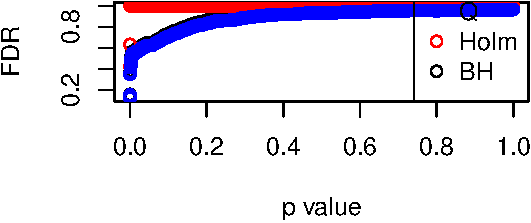
\includegraphics{sciguide_files/figure-latex/unnamed-chunk-17-1} \caption[谢林隔离模型模拟]{谢林隔离模型模拟}\label{fig:unnamed-chunk-17}
\end{figure}

个人群体的另一个重要模型是关于外部性或公共物品的,公共物品非排他也非竞争,其总效用函数是递减的,也就是后来的人可以享受公共物品但不用贡献,这会导致公共物品在人口增加后会紧缺但个人贡献意愿却因为后来者低贡献而降低。如果没有利他主义的人存在,公共物品或外部危机就会让群体不能持续维持正常运转。最常见的外部性解决方案就是税收或法律,如果不同群体间存在不同的税率会出现隔离与割裂,例如阶级固化后富人区内部大方而对外割裂,穷人区因为没有公共物品其法制也无法贯彻。单纯提供外部性并不一定会提高整体收益,存在反馈,更多的路引入了更多的车,阻塞问题可能依旧,系统分析是很有必要的,找出本质问题而不是解决表面问题。最麻烦的外部性问题是资源类问题,当资源开采速率超过一定速率后,平衡将不可逆走向崩溃,复活节岛就是一个例子,这类问题需要优先预防监控,不能等事情发生。当然,预防的悖论在于你做的越好,实际地位就越不重要。

群体间可通过机制设计来维持稳定,没有法律,社会会乱,下棋没有规则,游戏没有乐趣。机制要平衡个人多样性需求来实现整体最优,其中自愿、自发、低成本运行的机制(芒特-赖特尔图)是理想的,有些问题需要复杂规则设计来实现目的。例如在石头剪子布中,纳什均衡并不会有唯一解,有时纳什均衡不是整体最优。多数人投票中也存在这个问题,会出现投票中的独裁者,但拥王者机制则可实现整体最优,随机选一个人作为``拥王者'',这个人指定一个王来给出最终选择。又比如广告位拍卖,理性价位是价高者得的次高价,所以规矩就是如实报价然后按第二高价格卖给出价第一高的人。但事实上,不同拍卖规则下如果参与者都是理性的,最后实际价位应该是一样的,不过结果一致但听上去感受可能会不同,机制设计者要充分权衡。

文化差异也存在模型,文化是使群体生活与个人生活能进行的事物,国家文化差异客观存在,个体通过与他人协调与自己行为磨合形成,文化交汇会促进相似但不是一致。一致性会形成路径依赖与偏好加强,最后形成临界点。事物的发生靠技能也靠随机性,技能接近看的是运气。

关于个体与个体,个体与整体,整体与整体间行为的模型构建,博弈论给出了系统答案与解决策略。投票、选举、拍卖、联盟、反悔等一系列问题都是博弈论议题,说白了就是讲两方势力在一件事上为了自己的最大利益所采取的行动或决策的理论,是重要的模型思维工具。

\hypertarget{ux52a8ux529bux5b66ux6a21ux578b}{%
\subsection{动力学模型}\label{ux52a8ux529bux5b66ux6a21ux578b}}

前面的决策模型大都是静态决策,真实世界要考虑发展的过程,也就是动力学模型。事情的发展可以用马尔可夫模型来模拟,当状态有限且发生概率恒定时,事情就会进行状态改变直到收敛。概率转移矩阵就可以计算最终平衡时比例,因为是动态平衡,经常反线性直觉。这个过程跟初始状态无关,跟过程也无关,通过随机性达到平衡,但如果转移矩阵改变了,就可能不收敛了。

另一个事物发展模型是李雅普诺夫函数,它存在一个最大值或最小值,在没达到时会不断逼近,平衡时会停止波动,可根据构建的模型来估计逼近所需要的周期并优化。行为没有外部性会最终平衡,考虑外部性会复杂或随机,这个模型依赖路径与初始条件来达成平衡,平衡点固定不随机。例如美国所有州政府都倾向于削减社会项目支出的行为,因为会吸引外州穷人。

系统的发展会存在反馈与路径依赖,例如正反馈加强的波利亚过程,出现任何情况的概率是相同的,出现看似极端的情况并不意外。而均衡过程则不会产生路径依赖,是一种制衡。 路径依赖不同于临界点,熵的减少是均匀的而不是突然的。在系统中,有充足时间尝试的自组织会达到均衡。在构建系统动力学模型时,要考虑源头与汇,还有存量、流量、速率与常数。

\hypertarget{ux542fux53d1ux6cd5}{%
\section{启发法}\label{ux542fux53d1ux6cd5}}

启发法的较正式的解释是非最优非理性快速解决问题或作决策的方法,包括试错、经验法还有拟设(类似假设检验),类似直觉经验判断的混合体。一般包括两步,随机寻找与爬坡,随机寻找进行尝试,根据结果向着期望方向寻找直到达成目标或时间用尽。此时,使用者知道如何检测结果但不知道如何生成出现结果的机制。与启发式相对的是解析式问题(例如梯度优化),此时我们知道问题原因,可以根据原因来求解,例如有函数我们可以求导来算极值,而启发式则是只知道要求极值但函数未知,常用来解决黑箱难题。

启发法里也存在一组制衡:探索(exploration)与利用(exploitation)权衡。探索侧重复杂空间例如完全随机搜索,利用强调快速求解例如爬坡。启发法中一个关键步骤就是探索完一次得到继续探索信号后如何生成新参数,微小的参数改变有利于寻找方向而较大的改变有利于摆脱局部最优。也就是说在资源有限条件下,想更多探索解决方案空间就没法获取很高的求解精度,反之,在局部解决方法上反复优化就没法探索更大的解决方法空间。

不过,启发法本身的设计却可以很艺术的去探索两者的平衡。模拟退火算法的核心思想是在随机寻优结果是负面的时候也会以一定概率接纳,负面越高越不接纳,也就是尽可能引入改变来防止局部最优。禁忌搜索(tabu search)算法会预先设定一个列表,最优的结果都存到里面,存入后就不再考虑对应的参数修改方式,这个过程反复进行填满列表后最早的就可以踢出去重新考虑了。这也是防止局部最优的策略。迭代式局部搜索则从时间上做文章,先进行一段时间爬坡找到局部最优,然后进行较大的随机行走,在新位置上爬坡找最优,跟之前对比留下好的,然后继续迭代。

上面这些策略都可以用,也可以组合使用。除了这类单一状态优化外,另一类启发法则是从种群角度进行计算的,同时进行多组扰动,根据结果探索变化方向。这个思路来自生物学里的进化算法,包括遗传算法与进化策略。基本思路是设置初始种群,计算适应度,然后选一部分个体进行一代遗传,遗传过程伴随突变,之后重新计算适应度,最后留下适应度高的继续遗传。

种群初始化时要尽量多保持多样性,可以用哈希表来存储独立个体。在进化策略上,计算完个体适应度后只保留部分高适应度个体进行遗传,下一代数目与初始种群一致,例如每代10个个体,但只选2个最高适应度的遗传突变,下一代数量还是10个。当然,也可以在下一代里把第一代也都考虑进去进行筛选,如果一代不如一代,至少还保留了上一代的优良基因。突变率依赖正态分布的方差,经验法则就是如果多于五分之一子代表现更好,需要增加方差防止局部最优,如果少于则减少方差,等于则不变。

在遗传算法中,子代生成是有父母贡献一半进行杂交然后加上突变的,这里面多一个随机翻硬币来决定子代那一部分交换的步骤,此时遗传部分的可能性空间是确定的,另外杂交过程也可以对连续变量进行线性插值。在进行适应度选择上,可以根据概率去选,也可以用非参方法排序来进行选择。

在启发法特别是基于种群的启发法中,并行计算特别重要,你可以并行多组启发算法,或者在同一台机器多线程计算适应度,或者用分布式计算来分散汇总结果。如果需要多目标优化,就设计一个由多目标加权组合的新适应度指标。启发法也可以用在组合优化问题例如背包问题或邮差送信问题。此时可以先构建出一个组合,然后在有限时间内进行组分调整计算适应度,最后留下好的。蚁群优化则是先构建一组备选方案,然后计算适应度,记录各个组分的表现(信息素),重复这个过程,然后根据各组分信息素多少来选择最终组合。这个过程信息素可以挥发,备选方案也可以进行一定的爬坡,也可以用禁忌搜索来禁用掉一部分组分。同时随机数生成对于启发法也很重要。

多臂老虎机就是实际问题求解一个常见场景,多个备选方案与有限尝试次数是实际问题中常遇到的情况。我们可以利用贝叶斯方法先给每种方案一个先验收益,然后每尝试一次,更新一次期望收益,根据新的期望收益决定下一步尝试的方案,不断迭代。多臂老虎机可用来求解最佳方案,但算法实现需要足够尝试,否则新方案永远不会有出头之日。

了解启发法的相关算法对科研是有帮助的,因为科学问题的求解通常面临资源有限的情景,此时预实验或探索性数据分析就要借鉴启发式算法的思想,不仅仅优化自己熟悉成熟的解决策略,还有留足够的随机行走空间。时至今日,很多科学问题可以通过仿真手段来验证与求解,怎么设计一个探索性仿真策略也需要对启发式算法有一定的理解。

但最重要的是,启发法其实与认知偏误有时是伴生的,很多直觉性尝试都埋伏了认知偏误而容易导致陷入局部最优而不自知,而完全随机尝试的启发法其实是反直觉的。如果所有人都在用一套解题策略来攻克一个科学问题,那么尝试下从所有思路里随机选择可能会发现更好的解题策略,也就是要试错。不知道从什么时候开始,流行文化里对正确与成功的故事给予了很高的认可,很多人不能也不敢犯错,按部就班走流程排列组合在科研论文中形成了新八股的趋势。我们只能看到漂亮且显著的结果而不知道论文背后的试错过程,很多研究事实上脱离实际且不易重复,这种趋势会把科研人员的思路锁在那些四平八稳不犯错的研究而不是真正解决问题。须知,没了启发的研究就像是吃饺子不蘸醋/酱油/辣酱,入喉尚可但并不美味。

\hypertarget{exp}{%
\chapter{实验}\label{exp}}

有了思维工具就可以进行实验了。实验的基本任务包括描述现象、推断机理与预测验证。描述性实验或者说观察研究也是需要设计才能回答科学问题的,机理或验证实验则必须通过随机化与控制变量来设计。当科学发展到实验科学年代,统计学就要去解决刻意观察获得规律的方法。这里面随机化是一个核心观念,用来确保除了你关心的变量,其余的都能随机或符合某个分布。1874在《科学原则》这本书里首次提到了控制变量法,一次测一个。但在统计学大放异彩的20世纪,Fisher 认为一次回答一个问题是错的,因为自然问题从来都是复杂的不能只回答一个,提出了加性模型。这里统计学要为复杂现象提供合理的设计工具,时至今日,在数据概念满天飞的时代数据收集似乎不是问题,很多人就会说更重要的是提出问题。这倒没错,但如果没有统计学思维加持,很多问题是无法对应实际数据的,如果设计不当或有偏,拿到的现象就会产生误导。

不能为了设计实验而设计实验。例如,George Box 在《Statistics for experimenters》的第一章里是没有扯什么随机化、均匀性的,而是聊了下认识论。开篇第一句就是``知识就是力量'',解决问题实际就是一个认识模型演进的过程。具体来说是一个归纳-演绎不断往复的过程,数据起了中介作用。例如下面这个认识过程:

(模型)每天都一样

(演绎)今天车会停在原位

(数据)车不在

(归纳)有人偷车

(模型)车丢了

(演绎)车不在原位

(数据)车又回来了

(归纳)有人偷了车还回来了

具体到实验,这个过程就成了(模型)想法 -\textgreater(演绎)实验设计 -\textgreater(数据)结果分析 -\textgreater(归纳)结论或新想法。这大概是实验设计能上升到的最高理论高度了。不过,实验涉及的测量与分析方法对于科研提供经验事实非常重要,经常扮演理论的试金石,现代科研离不开实验结果支撑,且向自动化、模块化、定量化发展。实验学科的科研人员不必对工程技术细节完全掌握,但必须清楚其中测量原理与简单的故障诊断,否则实验就会黑箱化。

\hypertarget{ux601dux60f3ux5b9eux9a8c}{%
\section{思想实验}\label{ux601dux60f3ux5b9eux9a8c}}

这是科学实验里非常特殊的一种,通过预设场景进行推演得到结论。常见于物理学,但其他学科也\href{https://zh.wikipedia.org/wiki/\%E6\%80\%9D\%E6\%83\%B3\%E5\%AF\%A6\%E9\%A9\%97}{有}。有些思想实验是无法在真实世界操作的,例如拉普拉斯妖,有些则是可操作但技术或成本现阶段不经济,例如戴森球,还有些曾经是思想实验后来真的做出来的例如图灵测试。思想实验通常会引导出一个悖论或反直觉的现象,但这里的悖论是跟普通人的知识水平有关的,有些现象悖论确实就是事实,例如光的波粒二象性。

这里讨论下跟现代科研有关的几个思想实验。在中文房间的思想实验之中,我们假定一个完全不懂中文只懂英语的人被关在一个小屋里,里面有一本英文手册,里面用英文记录了一些汉字处理规则但没有说这是汉字,只是一些图像转换关系,此时外面一个懂汉语的在纸上写了一个汉语问题送到这个房间里,里面那个人根据英文手册把答复画出来(其实是中文)送出去,门外的人看到会以为里面有个懂中文的人,不过事实上里面那位都不知道自己画的是中文。这个思想实验跟图灵测试类似,都是人工智能里的经典命题,当手册换成程序,不懂中文的人换成计算机或服务器,我们能否说通过了图灵测试的机器具备了智能或者``知道''了一些事?有问有答是表面上的``知道'',但如果没有进一步提问,那么我们事实上无法区分``知道''的质量。

其实,从现代社会视角,``知道''的质量很多时候无关紧要。在现代教育体系中,培养的多数人才包括高等教育在内是机械化工具化的,其知识的应用程度很多时候就是有问有答即可。思想的深度并不是现代社会运转的必需品,很多时候还属于危险品。特别在分工体系里,在生理寿命与精力限制下个人事实上也不太可能``知道''太多,很多行业仅仅做到表面``知道''都很不容易了。我们的学习过程大都是构建在前人成果或结论而不是思考之上的,为了掌握知识迎合认知教育过程会省略过程直接给结论,或者在事后用漂亮的叙事逻辑线索串起来,但这样的后果就是我们需要掌握的知识越来越多但知识间产生联系的思想火花大都被掩盖了。分工前期有多促进效率,后期就有多降低效率,跨学科交流成本会因为分工制造的术语墙变得越来越高,而很多行业黑话本可以很直白的描述,甚至很多是从别的学科借过来的隐喻。

这对科研行业而言副作用非常大。现在实验学科发文章都需要用到统计学知识,但很多研究人员根本就没有理解统计概念而仅仅就是知道一个决策方法,例如p值小、R方高就是好之类,更不用说还有一批研究人员连好坏的判断标准都没有。但这其实不妨碍他们成为现代科研产业的从业人员,很多人只需要机械的进行实验然后把结果传给下一个只会数据分析的人生成一份几百页的报告就可以了,当然读报告的决策人员其实也只会去看看摘要里的p值跟R方。这套程序化操作倒是给后续检查留下了充足的材料,只是这些材料可能永远都没人读。那问题来了,这套程序究竟是给谁看的?超生命体?在现代社会的信仰者眼中,这是先进跟完备的体现,超越了人性的存在并忠实记录了发生的事,但可能真相是这样运转的行业能发工资养家糊口且权责清晰,哪怕根本解决不了科学问题。

其实关于这个``知道''问题哲学家也有定义,也就是所谓的JTB理论,认为A知道B的知识有三个要素,第一个是B本身为真,第二个是A相信B是真,第三个是A相信B为真这事是得到证实的。逻辑上看起来也似乎没啥问题,例如上面那个中文房间实验中只满足了后面两个,但不满足B本身为真这个条件。不过发表这个论文的哲学家当场就给了反例的思想实验,简化版就是A跟B竞争一个职位并两人同时买了彩票,A某天听上司说职位给了B,而且由于B学历高经验丰富A也相信了,但同时A听说B中了彩票,A就知道:得到职位的人中彩票了,但事实却是A的彩票也中奖了他还不知道。这里A知道的事满足知道三要素,但却是不全面的``知道'',不能形成知识。

要我说哲学家搞这么啰嗦还不如去看下斯金纳的迷信鸽子实验,实验人员设定一个隔十五秒就出食的喂食器喂鸽子,然后过了几天后发现,当喂食器不出食物的时候,有的鸽子原地打转、有的撞墙、有的摇头\ldots 鸽子们形成了一种只要做一件事15秒就有饭吃的迷信,也就是鸽子版的``知道''实验。鸽子的学习过程也满足三要素:摇头就有食物落下、鸽子相信这事、鸽子相信这事被实验证实,但实验人员好比上帝视角,会发现这种``知道''完全不靠谱。没有上帝视角的因果关系可能有用但跟真相可能差了十万八千里。

很多学科构建术语墙,用特定的生僻词来描述一个本可以形象描述的概念,用词本身的少见多怪来构建自己的专业性,但专业性需要的不仅仅是表面上的高深,而是真的知道。在科幻小说《基地》里,衰落的帝国的动力装置还有所谓的工程师在维护,但此时的工程师已经完全不知道装置运行的原理,仅仅是通过职位的专业性来维护自己的权威。如果有一天人类文明出现了衰退,那么知识精英的术语墙一定是其中的重要因素。

另一个重要的思想实验是无知之幕。所谓无知之幕,就是说你永远不知道下一个受害人是谁,因此保护措施就一定要按照下一个受害人是自己或自己的亲朋好友来设计。规则下的自由自由度最高,无序的自由一定造成意见割裂与对立。不过很多人也会去争论度的问题,如果搞不清度的把握,你可以问啊。什么都不说就按照自己的自由度聊天是不成熟的表现,尊重别人也会给自己赢得自由空间。现代科研体系里依然保留有导师-学生的等级制度,这使得导师与学生间的关系处理经常比较微妙,很多导师长于科研但弱于同理心,可能出现导师或学生一面倒只考虑自己然后两败俱伤的结局。无知之幕这样的规则设计原则尽最大可能考虑未来而不仅仅是眼下的公平,这对很多实验设计与科研思路也有启发,也就是通过更多的随机选择来避免研究上的有的放矢。

不过,信息时代无知之幕的现实基础正在被技术进步破坏。很多时候,有些人是知道自己不会成为受害者才肆无忌惮地争取利益。例如商品的差异定价,如果商家对你特别了解,它不会给你那个充分竞争的最低价,而是会根据你的消费水平推断出你能承受的最高价来维持自己的最高利润。而且你很有可能完全无法发现,这也是你在固定消费模式后决定的。个性化推荐的背后有着巨大的套利空间,此时游戏规则设计里如不考虑无知之幕或者通过技术与数据追踪突破了无知之幕,那么每个人将可能面临一个看似合理但实际被奴役的未来。在这样的空间里你的价值将被榨取到最后一滴而不自知,很多人则可能面临被侵害但上诉无门或彻底被主流声音所抛弃的境遇。对未来的无知是公平的最后一道保护伞,突破了这个,利益冲突就实质上成了社会伦理问题,这个时候有些人会成为社会的永恒弃子与棋子。但技术也可以用来巩固无知之幕,虽然事实公平很难保证,但起码在社会运行中,原则上给所有人公平自由的制度。

20世纪的技术进步是普惠的,21世纪的技术进步是优先照顾少数人的,因为技术研发成本越来越高。这就是那个挤公交问题,先上车的人上车后其实并不愿与后面上车的人均摊利益,有的恨不得把车门焊死来维护独占的利益。同时,最新技术造成的不平等也会越来越大,当一项技术无法从成本与资源上实现普惠时,社会割裂的可能性就很大了。所以,技术开发是要讲伦理的,优先开发普惠技术并在制度建设中维护无知之幕,否则弱肉强食的丛林法则会最终吞噬掉人类文明的基础。

了解思想实验最大的意义在于开拓眼界并学会悖论式思考,也就是通过形象化概念把一些规律性的矛盾展示出来。很多思想实验实际上是哲学家提出来的,思考这些实验可能也得不出什么唯一的结论,但这种不确定性的答案却是科学家面对科学问题经常需要给出的,思想实验对于训练科学家思辨能力很有帮助。

\hypertarget{ux4effux771fux5b9eux9a8c}{%
\section{仿真实验}\label{ux4effux771fux5b9eux9a8c}}

相比于思想实验纯粹的逻辑规律演绎,仿真实验则更多用于系统考察现象或考察系统特性。仿真实验的基础在于预定义个体或部分的属性与行为规则,然后在整体层面上观察现象。仿真实验的科研应用场景有两个:计算机辅助设计(CAD)与个体为本模型(ABM),前者更多用在工科研究中,例如工程力学上会通过建筑物建模来考察承重建材选择等问题,特别是没有解析解需要数值求解的问题,因为是计算机模拟,可以采集很多极端条件下系统承载参数;后者则更多出现在复杂性科学研究中,特别是博弈论与系统动力学考察,例如研究生态学种群变化规律就可以通过定义捕食规则与寿命,然后初始化一条食物链来研究系统的物质能量流动,例如生物圈二号。

仿真实验的三大基础是科学计算、机理与统计学。科学计算能力提升可以同时考察更多参数,更好模拟真实场景。新机理的提出与验证是多数仿真实验的目的,而已知机理的仿真则是模型的基础。统计学是仿真实验得到结论的工具,统计模拟可以帮助在未知规律的前提下展示提炼规律。相应的,仿真实验设计也要对科学问题的可计算性、原理与统计观测指标有清晰定义。

当前仿真实验的大趋势是虚拟化,越来越多的实验现在可以在计算机上模拟,小到分子动力学过程,大到谣言的网络传播机制都可以建模仿真。有机理则预设机理,机理不清楚就通过统计规律来揭示。越是接近真实的模拟,计算量与未知参量就越多,对经验公式与观察反馈也越高,甚至很多人认为人类就活在仿真程序里。

\hypertarget{ux89c2ux5bdfux5b9eux9a8c}{%
\section{观察实验}\label{ux89c2ux5bdfux5b9eux9a8c}}

观察实验是科学实验早期的主要形式,用无干涉观察来归纳总结规律,现在在社会科学或涉及人与伦理问题的科研中依然是主要方式。观察实验也需要设计,在流行病学或社会科学研究中,随机对照实验是最理想的但实际更多结论则是来自队列研究或断面研究。究其原因在于很多控制手段存在伦理问题,只能通过调查追踪的方式来进行。

当然,观察实验的科学问题侧重归纳性的规律总结,例如描述疾病在人群中的空间、时间分布或人群间属性例如年龄、性别、BMI、吸烟历史等的分布。为了观察数据可靠,就要有可靠的采样理论,在采样上或随机或均匀或分组布点,防止系统偏差。观察实验的难点在于观察数据不随机,这导致很多基于随机过程的统计推断无法展开甚至意识不到,观察实验的数据要很谨慎的纳入或排除可能的干扰因素,数据处理上就是对实际过程进行建模,用简化模型来控制影响因素,达到考察特定因素或指标变化规律的目的。

同时观察实验逻辑上也要解决现象的来源、过程与结束,这里面需要有科学问题。以持久性有机污染物的环境分析为例,我们首先观察到了持久性有机污染物的高山冷捕集现象,然后就要对这个现象进行析因,考察现象的每一个细节,例如污染物是哪里来的?本地生成还是外来输入?一次性输入还是持续输入?污染物发生了那些转化?形成了那些降解产物或加合物?最后污染物是会累积还是降解?相关过程动力学参数是什么?这个现象跟其他持久性有机污染物的研究有没有相关性?跟其他种类污染物的现象有没有区别联系?这里面观察实验如果给不出答案,就需要控制实验来验证了。上面这个例子的现象可以替换成其他学科的概念,对应科学问题也会有所不同。

伴随组学或大数据技术的出现,现代科研也需要更先进的观察研究方法论。在组学或大数据研究中,实验更多侧重数据挖掘而非设计,很多时候甚至要通过额外的数据处理手段来矫正观察数据的系统误差。在这类研究中,实验不是基于假设来设计的,随机性很难保证,要通过设立自我对照或配对来挖掘现象背后的规律。此时实验设计的思维要延续到数据处理中,更多相关问题我们会在下一章解释。

\hypertarget{ux63a7ux5236ux5b9eux9a8c}{%
\section{控制实验}\label{ux63a7ux5236ux5b9eux9a8c}}

与观察实验相对应的是控制实验,在控制实验的语境下,除了需要考察的过程或因素外所有其他因素都做随机化处理。控制实验一般有着明确的科学问题而最常见的控制变量法就是一组实验只考察一个因素的影响。如果打算同时考察多因素多水平的影响,可以理解为一个寻优问题,翻译成数学语言就是 \(y = f(x)\) 中,y代表了你期望最优的东西,x代表了会对y产生影响的自变量,如果你的问题可以抽象成 \(y = f(x)\),那就可以通过构建模型来解决,此时也就知道哪个影响更重要了。

所有的控制实验都要有对照组,且要根据实际需求设定不同种类的对照,例如阳性对照、阴性对照与空白对照等。对照组可能是反应测量精度的,也可能是为现象的描述提供基线数据。针对基线的对照设计要明白现实中的基线并不是完全随机的,或者说随机过程就可能产生一些现象规律而不是完全无现象,忽视这一点可能会误把偶然事件当成新规律,要克服认知上的错觉,从不同独立维度的验证或对基线的模拟是一定要做的。

临床试验类似控制实验,但要遵守\href{https://zh.wikipedia.org/zh-cn/\%E8\%B5\%AB\%E7\%88\%BE\%E8\%BE\%9B\%E5\%9F\%BA\%E5\%AE\%A3\%E8\%A8\%80}{《赫尔辛基宣言》}与\href{https://zh.wikipedia.org/wiki/\%E8\%B4\%9D\%E5\%B0\%94\%E8\%92\%99\%E7\%89\%B9\%E6\%8A\%A5\%E5\%91\%8A}{《贝尔蒙特报告》}来设计执行。互联网相关研究要遵守\href{https://aoir.org/reports/ethics3.pdf}{《Internet Research: Ethical Guidelines 3.0》}。

\hypertarget{ux56e0ux7d20ux9009ux62e9}{%
\section{因素选择}\label{ux56e0ux7d20ux9009ux62e9}}

对于特定科学问题,从哪里入手设计实验是需要谨慎思考的。我们的研究对象是单一物理实体,其影响因素要优先考虑其环境因素,基本出发点就是最基本的物理指标:长度,质量,时间,电流,热力学温度,物质的量和发光强度。所有的实验影响因素都应是这些物理指标组合而来,单位可以还原到这些物理指标的组合。描述因素影响上最基本的就是热力学与动力学描述。热力学描述可理解为现象稳态时的各种参数描述而动力学则关注现象在时间尺度上的参数变化。例如食盐在不同温度下溶解度就是其热力学描述,而固定温度下溶解过程中固态与溶解态的比例就是动力学描述。热力学与动力学过程涉及很多其他物理参数,但最常用的就是浓度或含量,特别是在不同温度、pH值与离子强度等环境参数条件下的热力学表现与动力学趋势。很多材料类论文的核心就是去表征新材料的各种属性参数,如果某项属性参数特别好,那么这种材料的现实意义也就特别高。

如果你研究的不是单一物质而是混合物,除了考虑热力学与动力学过程外还要考察混合物组分配比或组合方式对性质的影响。混合物可以是分子层面的,也可以是个体层面的,例如心理学或生态学上研究某些现象时不会只依赖单一个体的表现,但个体间组织方式也是影响某些心理现象的,例如是否来自同一家庭,是否是上下级关系等。此时在因素选择上要充分考虑哪些是不变的,哪些是可变的,或者说研究对象是否是均质的,否则不论是在实验设计还是数据分析阶段都要对相关因素进行控制。

同样的道理适用于对现象的研究。某个现象可能是复杂的个体关系与环境影响的结果,要搞清楚哪些是重要影响因素,哪些是可控制的,哪些是可是事后建模消除影响的。此时建议列个清单或者脑图,从现象内部到外部列出来所有因素,有些因素其实并不互相独立,此时要考虑如何建模消除掉非独立因素或整合为一个独立因素。

因素选好后就要考虑如果因素是分类的,那么不同分类的样本数能否平衡;如果因素是连续的,那么这个连续尺度是否在实际环境中存在。在更多情况下,控制实验的因素水平是事先选好的,这个水平可以推向极端来考察理论问题,但考虑实验的经济性与可重复性要优先考虑室温人居环境下存在的水平。例如考察污染物的对微生物的生态影响,其污染水平要跟环境中实际存在的污染水平相对应,否则做出的结果很难有实际意义。此外,现代技术进步使多维度同时考察变得可能,因素数也会变得越来越多,越来越复杂。此时要特别注意冗余分析,排除掉无关因素或实质等同的因素,避循环论证与被分析方法牵着鼻子走。

当然,前面所述思考方式是从头思考的,现代科研更多是建立在别人的工作上的,如果你并不是做的开创性工作,那么阅读类似文章对比论文结构可能是更实际的因素选择方式。这里还是要强调从头思考的重要性,因为这样可能发现前人所未想到的研究方向,而且一定也要去读别人的论文思考他们的思路,完全的闭门造车容易滑向民科的无底洞。

\hypertarget{ux6548ux5e94ux6307ux6807}{%
\section{效应指标}\label{ux6548ux5e94ux6307ux6807}}

实验设计要有明确的效应指标,可以是定性的,但最好是定量的。效应指标要简明直观去主观化,例如描述一种气味可以用文字,也可以用形成气味的物质比例,前者是一种感受,会带有主观差异,后者则是一种客观描述。各学科在发展中产生了很多专有指标,用来描述一些条件下有实际意义的过程与结果。现代指标体系很大程度是分析测量技术决定的,测量仪器给出的指标在对应研究领域内是相对通用的,从业人员要明白测量原理及故障应对方法,否则测量上如果存在问题就无法溯源与修正。

实验指标的构建可以是直接来自于测量本身,也可以是收取相关指标后续定义算法来计算。但无论如何测量数值都要有明确的物理意义,其背后也要有现实意义支撑,否则实验结果无法有效讨论。此外,指标还要保证信度与效度。所谓信度就是可靠性,也就是给出重现性好不确定性低的信号而不是随机信号,而效度要求则要保证指标可以反应所探索的问题。用体重秤来举例,高信度低效度的体重秤会给出一个稳定的数值,但这个数值却可能不是体重或总是系统高一个数,而低信度高效度的体重秤会给出一堆数值,虽然平均后是体重但测一次一个样,重现性不好。好的指标本身是依赖客观物理量但却能反应某个科学问题,例如水的总有机碳含量就可以指示或代表可燃成分的含量,同时可以用燃烧后测定质量的方式来得到高重现性的数值。

关于信度的考察要通过不确定性分析或信噪比分析。所有指标都有不确定度,一部分不确定度来自测量中引入的误差,还有一部分则可能来自指标本身组成就不稳定,例如心理学里对性格的定义。很多科学问题需要高分辨率数据,此时如果分析方法或指标噪声过多,那么也无法说明一些规律。

关于效度的考察要通过敏感度分析,看要指示的指标是否对想考察的问题能准确指示,这个时候一般会牵扯到``黄金标准''的概念。所谓黄金标准,就是行业内使用时间比较长,认可度最高的指标体系。新的指标要想说明优势,要去考察其相对黄金标准是否更好。打比方我们用卫星图像数据来对应空气质量,那么首先要用实地监测数据这种传统但可靠的方法来验证结果是否可靠,否则也许图像数据能给出很多数值,但完全偏离实测数据就没办法用。

现代科研经常需要定义或使用一些综合指标来简化指示某些复杂现象过程,例如空气质量指数。综合指标的设计要用到层级结构与加权,这些经验信息要么来自于理论,要么来自于现状调查,但要做到其确实可以指示量化复杂现象或过程。此外,综合指标要有能力分拆为独立不相干的子指标来进行深入的机理讨论,例如空气质量指数的基础就是几种污染物的实测数据。

总之,现代科研不排斥新的指标,新的指标也为描述新的现象与机理提供了途径,但新指标的构建一定要考虑信度与效度,否则实验结果或者会因为误差太大不能准确描述现象,或者根本就没有说明现象。

\hypertarget{ux91c7ux6837ux4e0eux6837ux54c1ux9884ux5904ux7406}{%
\section{采样与样品预处理}\label{ux91c7ux6837ux4e0eux6837ux54c1ux9884ux5904ux7406}}

现实科研的样品可能来自工业化生产,也可能来自自然界。样品收集与预处理不但是很多后续分析的必然步骤,也是最容易被忽视的误差来源。如同统计采样一样,现实样品采样要符合代表性与随机性且要根据想看到效应的大小预设样本量。真实采样中几乎一定会遇到各种意外,需要保证采样信息的完整记录,包括但不限于采样时间、地点、采样人、样品名称、样本储运要求与其他意外信息的备注。样品采集后应尽快分析,减少储运带来的不确定性,储存条件或者是低温或者是保持样品原有环境。不过,现代采样技术的一大趋势就是原位实时采样甚至是依赖物联网传感器的实时监测,这样的采样尤其需要事先设计好位置与校准流程,保证数据质量。

样品预处理是现代样品分析的重要步骤,要设置好过程空白等流程来进行分析过程的质量保证与质量控制。样品预处理一方面是为了让样品均质化稳定化,另一方面则是为分析过程服务的,例如减少对分析仪器的污染。样品预处理的趋势是自动化,不过要事先根据研究目的来评估已有自动化流程是否会影响或系统误差。然而,采样与样品预处理在很多时候由于考察问题的新颖性是做不到机器取代人工的,依然属于劳动密集型工作,适度的编程会有助于过程的自动化但现实问题的复杂需要人的干涉,特别是探索阶段。请做好文字记录或多媒体原始记录,这样更容易查找可能出现的问题。

\hypertarget{ux9884ux5b9eux9a8c}{%
\section{预实验}\label{ux9884ux5b9eux9a8c}}

如果条件允许,所有正式实验前可以进行预实验。预实验经常用来评价实验方法是否可靠,重复性如何,特别是在该实验从未操作过的时候用来熟悉流程。预实验的研究对象很多时候不是真实样品而是标准参考物质或基质空白。有时预实验也会在小样本上进行验证假设,如果有现象,则可以进行正式实验设计,如果没有则可以记录后中止实验。对于新手而言,预实验也是很好的训练机会,用来对全流程形成操作层面概念。越多的试错就越好保证正式实验的数据质量,因此预实验的打磨对于所有实验科学科研人员都是必修课。

然而,另一类预实验是为了节省正式实验的成本或者说实验条件优化。一般而言,想找出多因素的最优组合,第一步是要确定哪些因素重要而哪些因素不重要,这是PB(Plackett-Burman)设计的应用场景。在不考虑交互作用的前提下,通过PB设计的表头进行两水平试验,然后进行方差分析并可视化就可以筛选出重要因素了。PB设计的试验次数一定是4的倍数,而且最大适合因子数会比试验次数少1。打个比方,我打算找出9个因素中哪个影响目标最大,那么我的试验次数至少选12,下面是个演示(这里使用开源的\texttt{FrF2}包):

\begin{Shaded}
\begin{Highlighting}[]
\FunctionTok{suppressMessages}\NormalTok{(}\FunctionTok{library}\NormalTok{(FrF2))}
\FunctionTok{pb}\NormalTok{(}\DecValTok{12}\NormalTok{,}\AttributeTok{nfactors =} \DecValTok{9}\NormalTok{)}
\end{Highlighting}
\end{Shaded}

\begin{verbatim}
##     A  B  C  D  E  F  G  H  J
## 1  -1  1  1  1 -1 -1 -1  1 -1
## 2   1  1 -1  1  1  1 -1 -1 -1
## 3   1  1  1 -1 -1 -1  1 -1  1
## 4  -1 -1 -1  1 -1  1  1 -1  1
## 5  -1 -1  1 -1  1  1 -1  1  1
## 6   1 -1 -1 -1  1 -1  1  1 -1
## 7  -1  1 -1  1  1 -1  1  1  1
## 8   1  1 -1 -1 -1  1 -1  1  1
## 9  -1  1  1 -1  1  1  1 -1 -1
## 10  1 -1  1  1 -1  1  1  1 -1
## 11  1 -1  1  1  1 -1 -1 -1  1
## 12 -1 -1 -1 -1 -1 -1 -1 -1 -1
## class=design, type= pb
\end{verbatim}

这里面1与-1分别代表两个水平,当然试验设计牵扯到分辨率问题,可以理解为对该试验设计的评价,分辨率高,能区分的影响就更细致,可以用\texttt{FrF2}包中的\texttt{GR}函数来计算实验设计的广义分辨率。例如刚才那个设计的分辨率就是 3.67。需要注意的是,\texttt{FrF2}包也可以用 \texttt{FrF2} 函数来进行两水平试验设计,这里分辨率高时是可以考察交互作用的。

那么当你收集了实验数据,该如何分析呢?\texttt{FrF2}包里可以用 \texttt{add.response} 函数增加你的试验结果到设计出的S3对象上,然后就可以用方差分析或线性回归进行分析了。结果同样可以用\texttt{MEPlot}函数来进行可视化。当然,也可以用\texttt{halfnormal}函数来评价因子影响。

\begin{Shaded}
\begin{Highlighting}[]
\NormalTok{plan.annotated }\OtherTok{\textless{}{-}} \FunctionTok{pb}\NormalTok{(}\DecValTok{12}\NormalTok{,}\AttributeTok{nfactors =} \DecValTok{9}\NormalTok{)}
\NormalTok{response }\OtherTok{\textless{}{-}} \FunctionTok{c}\NormalTok{(}\DecValTok{35}\NormalTok{, }\DecValTok{36}\NormalTok{, }\DecValTok{38}\NormalTok{, }\DecValTok{39}\NormalTok{, }\DecValTok{37}\NormalTok{, }\DecValTok{36}\NormalTok{, }\DecValTok{39}\NormalTok{, }\DecValTok{37}\NormalTok{, }\DecValTok{41}\NormalTok{, }\DecValTok{32}\NormalTok{, }\DecValTok{42}\NormalTok{, }\DecValTok{37}\NormalTok{)}
\NormalTok{plan.resp }\OtherTok{\textless{}{-}} \FunctionTok{add.response}\NormalTok{(plan.annotated, response)}
\FunctionTok{MEPlot}\NormalTok{(plan.resp, }\AttributeTok{abbrev =} \DecValTok{5}\NormalTok{, }\AttributeTok{cex.xax =} \FloatTok{1.6}\NormalTok{, }\AttributeTok{cex.main =} \DecValTok{2}\NormalTok{)}
\end{Highlighting}
\end{Shaded}

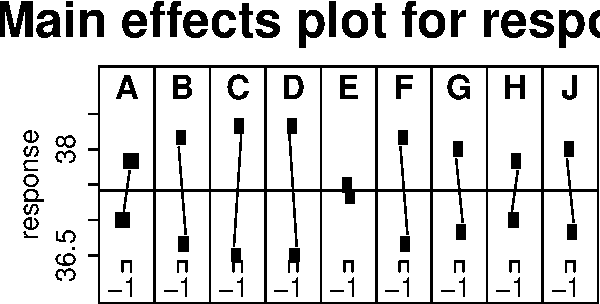
\includegraphics{sciguide_files/figure-latex/pba-1}

\begin{Shaded}
\begin{Highlighting}[]
\FunctionTok{summary}\NormalTok{(}\FunctionTok{lm}\NormalTok{(plan.resp))}
\end{Highlighting}
\end{Shaded}

\begin{verbatim}
## Number of observations used: 12 
## Formula:
## response ~ A + B + C + D + E + F + G + H + J
## 
## Call:
## lm.default(formula = fo, data = model.frame(fo, data = formula))
## 
## Residuals:
##       1       2       3       4       5       6       7       8       9      10 
##  0.1667 -0.1667 -0.1667 -2.0000  2.0000 -0.1667  0.1667 -2.0000  2.0000 -2.0000 
##      11      12 
##  2.0000  0.1667 
## 
## Coefficients:
##             Estimate Std. Error t value Pr(>|t|)    
## (Intercept)  37.4167     1.0035  37.287 0.000718 ***
## A1            0.7500     1.0035   0.747 0.532743    
## B1            0.5833     1.0035   0.581 0.619812    
## C1           -0.2500     1.0035  -0.249 0.826506    
## D1            0.2500     1.0035   0.249 0.826506    
## E1            1.0833     1.0035   1.080 0.393212    
## F1           -0.2500     1.0035  -0.249 0.826506    
## G1            0.7500     1.0035   0.747 0.532743    
## H1           -1.2500     1.0035  -1.246 0.339021    
## J1           -0.4167     1.0035  -0.415 0.718282    
## ---
## Signif. codes:  0 '***' 0.001 '**' 0.01 '*' 0.05 '.' 0.1 ' ' 1
## 
## Residual standard error: 3.476 on 2 degrees of freedom
## Multiple R-squared:  0.6938, Adjusted R-squared:  -0.6843 
## F-statistic: 0.5034 on 9 and 2 DF,  p-value: 0.807
\end{verbatim}

\begin{Shaded}
\begin{Highlighting}[]
\FunctionTok{halfnormal}\NormalTok{(plan.resp)}
\end{Highlighting}
\end{Shaded}

\begin{verbatim}
## no significant effects
\end{verbatim}

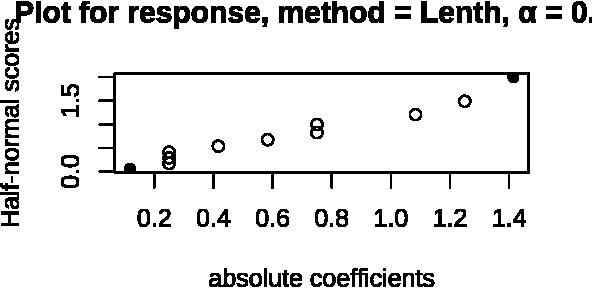
\includegraphics{sciguide_files/figure-latex/pba-2}

从上面的结果可以看出,我们九因素两水平的实验结果无法发现明显影响因素。在这里PB设计实际上是一种预选法,如果结果显示某些变量影响显著,那么事实上就可以针对这些变量进行进一步的精细筛选,其余的变量可以直接固定为一个水平进行进一步设计。

PB法在工业场景里用的比较多,但你应该想到了,如果只是进行变量选择,为啥不用随机森林或lasso?其实都可以,但这些方法不是设计而更多是数据分析通用方法,设计上除了最重要的随机性也是要考虑各因子贡献或者说重复数尽量平衡些的,否则会过分偏重某个因子,或者干脆配对或组成区组。像这样不做预设去设计对各个因子都公平,如果有预设或现实条件不允许,也可以裂区设计。

当选出重要因素时,下一步常见是正交试验或响应面分析,用来优选参数。正交表这玩意文献里用得多的也是亚洲人,老外统一用析因试验来描述这个考察过程。其实正交表的设计原理就是用尽量少的步骤遍历掉因子空间,这样进行一定次数试验就可以发现最优组合。R中的实现基本都在\texttt{DoE.base} 包里,这个包内置了一堆可以直接调用的正交表,可以根据需求进行查询。例如我有6个因素,水平数分别是2,3,3,2,2,6,然后我只打算做不超过54次试验,这时可以直接调用\texttt{show.oas}函数进行查询,给出的正交表随意选一个就可以继续。

\begin{Shaded}
\begin{Highlighting}[]
\FunctionTok{show.oas}\NormalTok{(}\AttributeTok{nruns =} \FunctionTok{c}\NormalTok{(}\DecValTok{0}\NormalTok{, }\DecValTok{54}\NormalTok{), }\AttributeTok{nlevels =} \FunctionTok{c}\NormalTok{(}\DecValTok{2}\NormalTok{, }\DecValTok{3}\NormalTok{, }\DecValTok{3}\NormalTok{, }\DecValTok{2}\NormalTok{, }\DecValTok{2}\NormalTok{, }\DecValTok{6}\NormalTok{), }\AttributeTok{showmetrics =} \ConstantTok{TRUE}\NormalTok{)}
\end{Highlighting}
\end{Shaded}

\begin{verbatim}
## no suitable  resolution IV or more  array found
## 5  orthogonal  arrays found
##                name nruns lineage   GR GRind regular SCones    A3    A4   A5
## 78 L36.2.13.3.2.6.1    36         3.00  3.00   FALSE      6  45.3 158.4  426
## 81 L36.2.10.3.8.6.1    36         3.18  3.18   FALSE      0 130.3 737.2 3063
## 83  L36.2.9.3.4.6.2    36         3.00  3.00   FALSE     17  82.3 338.2 1025
## 87  L36.2.3.3.9.6.1    36         3.18  3.00   FALSE     12  73.8 300.2  912
## 88  L36.2.3.3.2.6.3    36         3.00  3.00   FALSE     37  35.6  73.1  120
##       A6      A7      A8
## 78  1010  1753.2  2306.8
## 81 11096 31380.8 68828.1
## 83  2828  5507.5  7780.0
## 87  2404  4354.2  5793.4
## 88   125    63.5    13.9
\end{verbatim}

这里我们选分辨率略高的\texttt{L36.2.10.3.8.6.1},从名字上看,这是一个36次试验表,可以包含10个两水平,8个三水平与1个六水平因子,这也是唯一一个分辨率高于3,可以排除交互作用的设计方法。这里我反复提到分辨率,实际上就是一种考察试验设计合理性的指标,分辨率3一般指只能区分没有交互作用的各因子贡献差异,高于3就可以区分一定的因子交互作用,可以用\texttt{GR}去计算一个广义分辨率并用\texttt{oa.design}来进一步优化这个设计,因为其实符合正交表只是众多选择的一个子集,不过根据优化方法的不同,优化时间也不太一样。

\begin{Shaded}
\begin{Highlighting}[]
\CommentTok{\# 设计一个三因素三水平的实验}
\NormalTok{test }\OtherTok{\textless{}{-}} \FunctionTok{oa.design}\NormalTok{(L36.}\DecValTok{2}\NormalTok{.}\DecValTok{10}\NormalTok{.}\DecValTok{3}\NormalTok{.}\DecValTok{8}\NormalTok{.}\FloatTok{6.1}\NormalTok{, }\AttributeTok{nlevels =} \FunctionTok{c}\NormalTok{(}\DecValTok{3}\NormalTok{, }\DecValTok{3}\NormalTok{, }\DecValTok{3}\NormalTok{),}\AttributeTok{columns =} \StringTok{"min34"}\NormalTok{)}
\end{Highlighting}
\end{Shaded}

使用这个函数你就不用费力去套正交表了,直接可以用输出的设计方案,记得要说明你的分辨率优化方案。如果你坚持套正交表,一定要理解如何去套,因为正交表的排列是很讲究的,特别是你要考虑交互作用的影响。如果一个表最多14个因子而你就设计了14个因子,那么分辨率不会超过3。正交设计的分析与前面PB设计是一致的,都是沿用添加响应,然后方差分析或线性分析随意来就是了,\texttt{DoE.base} 包为\texttt{design}这个表示实验设计的对象类型设置了方差分析或线性分析的分析方法。

\begin{Shaded}
\begin{Highlighting}[]
\FunctionTok{oa.design}\NormalTok{(L36.}\DecValTok{2}\NormalTok{.}\DecValTok{10}\NormalTok{.}\DecValTok{3}\NormalTok{.}\DecValTok{8}\NormalTok{.}\FloatTok{6.1}\NormalTok{, }\AttributeTok{nlevels =} \FunctionTok{c}\NormalTok{(}\DecValTok{2}\NormalTok{, }\DecValTok{3}\NormalTok{, }\DecValTok{3}\NormalTok{, }\DecValTok{2}\NormalTok{, }\DecValTok{2}\NormalTok{, }\DecValTok{6}\NormalTok{), }\AttributeTok{columns =} \StringTok{"min34"}\NormalTok{)}
\end{Highlighting}
\end{Shaded}

\begin{verbatim}
##    A B C D E F
## 1  2 3 3 2 1 6
## 2  1 2 1 1 2 4
## 3  2 2 2 1 2 1
## 4  1 2 2 2 2 2
## 5  2 1 2 1 1 6
## 6  2 1 1 2 1 2
## 7  2 1 2 1 2 4
## 8  2 1 3 2 1 3
## 9  2 1 1 1 2 5
## 10 1 3 3 1 1 5
## 11 1 2 3 2 2 5
## 12 2 3 3 1 2 3
## 13 2 3 1 1 1 4
## 14 1 2 3 1 1 1
## 15 1 1 1 2 2 6
## 16 2 3 2 2 1 1
## 17 1 2 2 1 1 3
## 18 1 3 3 2 2 4
## 19 1 2 1 2 1 6
## 20 1 3 1 2 2 1
## 21 2 2 2 2 1 4
## 22 2 2 1 2 2 3
## 23 2 1 3 2 2 1
## 24 1 1 3 1 2 2
## 25 2 2 3 1 2 6
## 26 1 1 2 1 1 5
## 27 1 1 1 1 1 1
## 28 2 2 3 1 1 2
## 29 1 1 3 2 1 4
## 30 1 1 2 2 2 3
## 31 2 2 1 2 1 5
## 32 1 3 1 1 1 3
## 33 2 3 2 2 2 5
## 34 1 3 2 1 2 6
## 35 1 3 2 2 1 2
## 36 2 3 1 1 2 2
## class=design, type= oa
\end{verbatim}

\begin{Shaded}
\begin{Highlighting}[]
\CommentTok{\# 这里我们故意设计一个A因素无影响,B与C因素有影响但C影响大的响应}
\NormalTok{response }\OtherTok{\textless{}{-}} \FunctionTok{apply}\NormalTok{(}\FunctionTok{as.data.frame}\NormalTok{(test),}\DecValTok{1}\NormalTok{,}\ControlFlowTok{function}\NormalTok{(x) }\FunctionTok{sum}\NormalTok{(}\FunctionTok{as.numeric}\NormalTok{(x)}\SpecialCharTok{\%*\%}\FunctionTok{c}\NormalTok{(}\DecValTok{0}\NormalTok{,}\DecValTok{20}\NormalTok{,}\DecValTok{100}\NormalTok{)))}
\NormalTok{test.resp }\OtherTok{\textless{}{-}} \FunctionTok{add.response}\NormalTok{(test, response)}
\FunctionTok{summary}\NormalTok{(}\FunctionTok{aov}\NormalTok{(test.resp))}
\end{Highlighting}
\end{Shaded}

\begin{verbatim}
## Number of observations used: 36 
## Formula:
## response ~ A + B + C
##             Df Sum Sq Mean Sq   F value Pr(>F)    
## A            2      0       0 2.120e+00  0.138    
## B            2   9600    4800 4.776e+30 <2e-16 ***
## C            2 240000  120000 1.194e+32 <2e-16 ***
## Residuals   29      0       0                     
## ---
## Signif. codes:  0 '***' 0.001 '**' 0.01 '*' 0.05 '.' 0.1 ' ' 1
\end{verbatim}

\begin{Shaded}
\begin{Highlighting}[]
\FunctionTok{summary}\NormalTok{(}\FunctionTok{lm}\NormalTok{(test.resp, }\AttributeTok{response =} \StringTok{"response"}\NormalTok{))}
\end{Highlighting}
\end{Shaded}

\begin{verbatim}
## Warning in summary.lm(object): essentially perfect fit: summary may be
## unreliable
\end{verbatim}

\begin{verbatim}
## Number of observations used: 36 
## Formula:
## response ~ A + B + C
## 
## Call:
## lm.default(formula = fo, data = model.frame(fo, data = formula))
## 
## Residuals:
##        Min         1Q     Median         3Q        Max 
## -1.214e-13 -7.130e-15  5.948e-15  1.444e-14  4.553e-14 
## 
## Coefficients:
##               Estimate Std. Error    t value Pr(>|t|)    
## (Intercept)  2.400e+02  5.284e-15  4.542e+16  < 2e-16 ***
## A.L          2.210e-14  9.152e-15  2.414e+00  0.02230 *  
## A.Q         -2.089e-14  9.152e-15 -2.282e+00  0.03001 *  
## B.L          2.828e+01  9.152e-15  3.091e+15  < 2e-16 ***
## B.Q          2.130e-15  9.152e-15  2.330e-01  0.81757    
## C.L          1.414e+02  9.152e-15  1.545e+16  < 2e-16 ***
## C.Q          3.119e-14  9.152e-15  3.408e+00  0.00194 ** 
## ---
## Signif. codes:  0 '***' 0.001 '**' 0.01 '*' 0.05 '.' 0.1 ' ' 1
## 
## Residual standard error: 3.17e-14 on 29 degrees of freedom
## Multiple R-squared:      1,  Adjusted R-squared:      1 
## F-statistic: 4.139e+31 on 6 and 29 DF,  p-value: < 2.2e-16
\end{verbatim}

\begin{Shaded}
\begin{Highlighting}[]
\FunctionTok{plot}\NormalTok{(test.resp)}
\end{Highlighting}
\end{Shaded}

\begin{verbatim}
## The first four factors were selected. Use argument select for choosing what is plotted.
\end{verbatim}

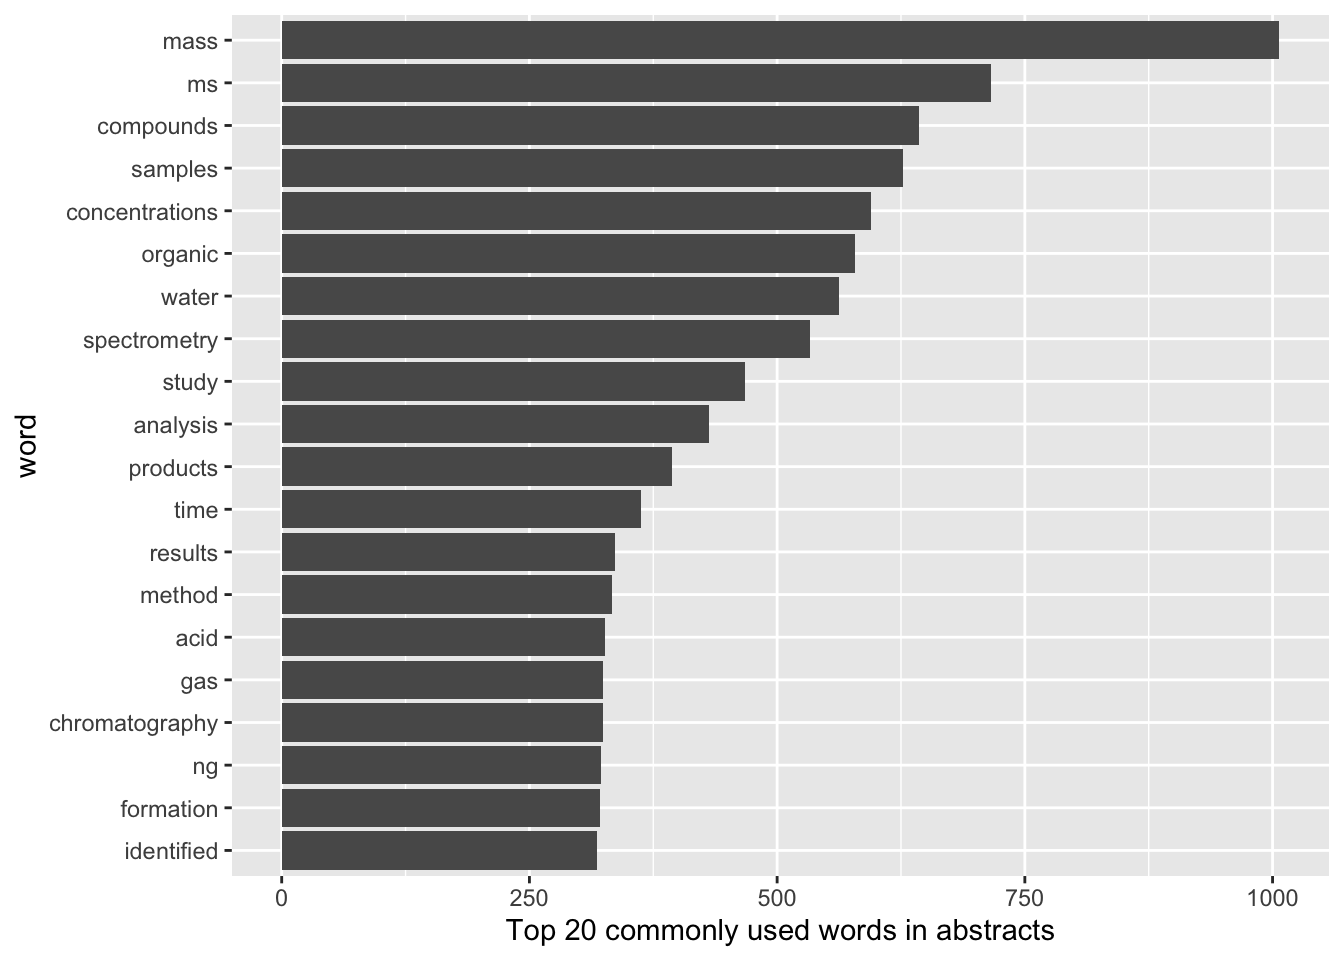
\includegraphics{sciguide_files/figure-latex/unnamed-chunk-20-1}

这里我们可以看出结果与我们设计的响应是能对应上的,也能从图上看出哪个影响更大。在进行数据分析时,有时会遇到方差分析与线性回归的区别问题,打比方你用线性回归来做分析,会有审稿人问你 lack of fit 检验有没有做。这个检验实质上也是个F检验,用来衡量线性模型之外残差里分组变异与纯误差变异的比值,如果分组变异还是比较大,那么线性假设可能就不合理。

不过,目前实验设计结果分析更精细的会用响应面分析。顾名思义,响应面有点梯度下降迭代寻优的意思,而且如果是曲面通常考虑了二阶甚至更高阶的交互作用,可以看做多元函数的高阶泰勒展开。在R中可以通过 \texttt{rsm} 包来进行的,这个包也是囊括了设计与分析两个部分,设计部分有常见的 Box-Wilson Central Composite Designs(CCD) 与 Box-Behnken designs,分析部分自然还是基于线性回归或方差分析那一套。好的CCD设计意味着一些表征设计均衡的因素与水平统计量。

这里要清楚不论正交表还是响应面分析,都不会是一锤子买卖,第一批实验数据出来以后马上进行分析,然后找出较好的因素与水平,之后再以此为中心设计第二批实验,不断反复直到待优化的指标不再产生变化。如果你面临多响应同步优化问题也可以进行优化,例如R中开源\texttt{desirability}包就可以处理这个问题,本质上是定义了一个多响应的联合满意度作为目标统计量,然后用响应面分析进行寻优。另外说个小八卦,狭义正交表也就是田口设计其实最初是两响应优化,只不过另一个响应是无法控制的噪声,田口搞了个信噪比来解决问题,熟悉了这套统计量构建策略,你也应该能做到根据实际情况构建指标体系。

其实实验设计分析是可以用所有符合\(y = f(x)\)的模型来操作的,说白了就是参数寻优。但试验设计更独特的点就在设计上,更广义地讲,A/B测试等纯计算试验也可以套用试验设计原理,这里要区分清楚设计与分析,设计不合理,分析会很头痛。如果再扩展些,观察研究的试验设计相比控制实验更关注配对或策略抽样。总之试验设计并不是什么水晶球,其原则从来都很清楚,只是后来流派出的太多,术语也越来越晦涩。然后你就会在网上看到哪个软件能做哪个分析的讨论了,其实这情况在工科可能更严重些,例如混料配比的\href{https://support.minitab.com/zh-cn/minitab/18/help-and-how-to/modeling-statistics/doe/supporting-topics/mixture-designs/what-is-a-mixture-design/}{三角坐标系设计}就完全是另一套,不过万变不离其宗,说白了还是个响应面分析。

\hypertarget{ux8d28ux91cfux4fddux8bc1ux8d28ux91cfux63a7ux5236}{%
\section{质量保证/质量控制}\label{ux8d28ux91cfux4fddux8bc1ux8d28ux91cfux63a7ux5236}}

科研实验中质量保证/质量控制是分析化学里的概念,但现在的实验学科大都接纳了这个概念,用来描述实验整体的可靠性,特别是过程控制。科技论文的实验方法部分一般会有一个独立章节来描述质量保证/质量控制的细节。其中,质量保证是验证整个实验的过程中误差是可接受的而质量控制指用一些手段去检测实验中的误差,前者侧重流程端预防保证实验质量而后者则是则是从结果端评价控制实验质量。这两个概念很接近,实际实验过程中都是通过一些特定的措施来实践。

质量保证流程需要给实验人员设计标准操作流程(Standard operation procedure,SOP)来预防实验人员流动带来的结果差异。同时,实验室需要对新人有充足的培训及对分析仪器有专业的维护并且对实验过程有完整的日志系统追踪。此外,较严格的实验室还需要年检与盲测,要有报告可以追踪。这部分内容通常不会体现在论文里,但论文出问题的时候这部分内容是要拿出来核查的。

质量控制则更多体现在前面所说的控制实验里,也就是要有各类对照、标准参考物质、加标样品、实验室平行测样等。各类对照是为了防止外来干扰与设定对比基线,没有对照根本就称不上控制实验。标准参考物质则是一类各个实验室都能获得的由权威机构认证过的样品,通常有认证过的物质含量,这样测定标准参考物质中已知物质的含量就可以很好评价实验室整体的操作水平。加标样品类似,通过在样品中加入已知含量的物质,然后利用该物质的测定波动校准类似结构的物质的定性与定量。实验室平行测样是构建分析方法标准的一个必须步骤,不过对于科研问题,让协作者在不同实验室测定同样现象进行对比有时候也可以更好保证结果的可靠性,不然跟家庭作坊也没啥区别。

这里特别强调一下重复性,重复性是用来保证结果不是随机的,不同学科要求不一样,至少三遍且结论都一致的结果可信度高。这里的``三遍''指的是整体实验的重复,由这个结果出的不确定度来可以估计结果的真实性。但每次实验之中也有重复,例如测量长度测至少三遍或五遍,这个重复是技术性重复,通常衡量的是分析方法,最后论文或报告只会用到均值,另外一种重复是生物性重复,也就是测定不同的生物样品里同一个指标,此时描述的是生物指标本身在生物体内的均值与不确定度,这个是与控制实验的科学问题相关的。

举个例子,我们想评价A细胞暴露在甲污染物下活性氧浓度,此时为了保证活性氧浓度结果可靠我们同一个细胞样品测定六次取均值,这个是技术性重复;我们培养五组同样的A细胞,得到30个数值但其实只能用每个样本的均值也就是五个活性氧浓度六次重复测定的均值的均值与方差来描述A细胞暴露甲后活性氧的浓度,这个浓度与对照组进行比较是直接回答科学问题的。然而,更严谨的做法需要把整个过程重复三遍,如果三遍结果都一致,那么这个现象可能是真的。受限于实验成本等因素,很多研究只重复了一次,这时结果可信度就差一点。很多人经常搞不清技术性重复与生物性重复混用两个概念,后果就是测的数据很多但都来自几个样品的重复测量,最后评价的事实上是分析方法是否靠谱而不是结果是否靠谱。

不过就算是评价实验分析方法也要注意区别衡量的是仪器本身的可靠性还是整个分析方法的可靠性。测定结果的检出限就有两种,仪器的检出限是绝对的量,但整个分析方法考虑上样品内部干扰与前处理步骤给出的方法检出限通常是浓度这类基于样品的数值。例如我的仪器能测出10纳克某物质的量或者说进样量10纳克就能看到信噪比高于三的信号,这个数是绝对量,如果我样品1克,最后经过前处理在仪器上看到一个某物质信噪比刚好过三的信号,那么该物质的方法检出限针对该样品为10纳克每克,也就是10ppm。不过,如果我前处理可以浓缩样品中这个物质10倍,例如有机溶剂萃取后原来浓缩到100微升进样2微升,现在我浓缩到20微升进样4微升,那么测量同样信号(10纳克绝对量)就只需要0.1克样品,此时仪器检出限不变但方法检出限可以降到1ppm。

具体到论文的实验质量保证/质量控制章节,一般要报告对照实验的设计状况、分析方法的检出限与可信定量范围还有关于实验重复性的描述例如技术性重复的相对标准偏差等。也就是告诉读者,我这组实验的可靠性如何及哪些结果是可靠性高的,这部分需要一些统计量指标,要根据各学科内容来定。

\hypertarget{data}{%
\chapter{数据处理}\label{data}}

数据处理是科研中很重要的一环,同样的实验或观察数据不同的人处理会得到不同的结论。事实只有一个,但解释可以有很多,数据处理方式本身就会对解释产生影响。本章先讨论探索性数据分析,然后讨论统计推断的过程,之后解释线性模型与模型组合,因为科研中数据分析基本就是这几部分的反复迭代。然后讨论下现代科研中涉及的一些计算方法与技术,最后一节通过主成分分析把前面这些数据处理概念串起来讨论一下。

\hypertarget{ux63a2ux7d22ux6027ux6570ux636eux5206ux6790}{%
\section{探索性数据分析}\label{ux63a2ux7d22ux6027ux6570ux636eux5206ux6790}}

数据处理的第一步是探索性数据分析。本质上,所有数据分析都是从数据中挖掘规律,在有明确假设驱动的研究中,规律的探索是与数据收集实验设计紧密结合在一起的。探索性数据分析这对于观察数据或监测数据尤为重要,但对于假设驱动研究的数据探索性数据分析也有助于发现未预期的现象或进行故障诊断。探索性数据分析需要摒弃固有分析模式,用从头开始的思路对数据进行探索,可视化等手段有助于直观进行探索性数据分析。

所谓从头开始,就是从对数据本身的描述开始。基本的原则是:

\begin{itemize}
\tightlist
\item
  一维数据看分布与异常值
\item
  二维数据看关系与趋势
\item
  三维看维度间两两关系
\item
  高维数据降维
\item
  相似个体聚类与网络结构
\end{itemize}

这些原则的核心就是对数据中规律性的本质进行直观展示,也因此可视化手段尤为重要。

对于一维数据,均值、中位数等单一数值常在媒体报道跟论文中用来指代群体,但其实牺牲了很多重要的分布细节进而产生误导,甚至让人产生被平均的感受,而直接展示整体其实并不困难,重要的是作者/研究者应放开心态,从引导读者认同自己观点转为让读者自己探索出\href{http://flowingdata.com/2017/07/07/small-summary-stats/}{结论}。一维数据可以被抽象为单一数值,但更可能是多种基础分布的叠加,探索性分析就是要从中找出数据中均质性与异质性。此外,一维数据会存在异常值,这些异常值可能需要其他数据来探索出现的原因,也可能仅仅就是随机出现,这时候大样本量会有帮助。一维数据的可视化方式一般为直方图或概率密度曲线或箱式图等。

二维数据如果不是坐标,那么优先考察样本中两个维度描述的关系,特别是存在时间这个维度时,考察的就是动力学过程,动力学过程一般会存在自相关,也就是相邻时间采集数据会接近,并不是独立的,此时可考虑求导数,不仅一阶导数,更高阶的导数也可以考虑。如果是坐标,那就要展示到平面上看下空间分布的离散情况,有没有聚集或其他趋势,然后可引入其他维度来寻找原因。二维数据可视化方式为散点图、折线图、地图等,要辅助一维展示方式来保留更多的细节。

三维数据可视化其实也是通过二维展示的,可以分拆为两两的二维数据关系来探索,或者用透视的方式来展示。另外常见的三维数据可视化方式是引入除了坐标外的其他展示要素来二维展示其他的维度,例如通过颜色、大小、长度、宽度等,例如热图。也可以单纯用柱形图或雷达图来并列展示多个维度。不过当维度不断增长后,同时展示多维度会造成阅读困难,这与探索分析的初衷违背,此时要分而析之而不是盲目追求可视化的复杂度。

高维数据的探索需要先降维,基本思路是趋势相对一致的维度重新整合为一个独立维度,提取出一个新维度。最常见的降维方式是主成分分析或因子分析,可理解为通过坐标轴映射让方差方向相对一致的因子重组为单一因子。另外的降维方式则有流形分析的一些技术例如 t-SNE、UMAP或基于人工神经网络的SOM等,都可以用来非线性降维。这里一定要清楚降维的前提是维度间存在某种相似性可以被降维,如果都是相对独立的,例如第一主成分对方差解释连5\%都不到,那么优先要做的不是降维,而是冗余分析,把不相关的维度先筛掉。大量不相关的维度会增加数据整体方差且降低发现真正规律的统计方法功效,因此不要盲目迷信方法,根据探索的方向来保留有意义的数据维度。

除了在样品维度上进行探索,样本间的关系可能也不是独立的。此时可以引入聚类分析来探索样本间的关系,聚类分析的核心在于样品间距离的定义,要根据数据本身的情况来定,但欧式距离比较常见。除了聚类分析,也可以考虑探索样本间层级关系或更一般的网络关系,此时要定义好层级间或节点间的连接条件,例如最常见的相关性,这样就可以对样品间的相互关系进行探索,看是否存在样本聚类的情况。当然,该方法也可用来探索维度间关系。

下面演示下常见可视化方法:

\begin{Shaded}
\begin{Highlighting}[]
\CommentTok{\# 读入鸢尾花数据集,150个样本及其花萼长度/宽度,花瓣长度/宽度还有种属}
\FunctionTok{data}\NormalTok{(}\StringTok{"iris"}\NormalTok{)}
\CommentTok{\# 一维可视化花萼长度}
\FunctionTok{hist}\NormalTok{(iris}\SpecialCharTok{$}\NormalTok{Sepal.Length, }\AttributeTok{xlab =} \StringTok{\textquotesingle{}花萼长度\textquotesingle{}}\NormalTok{, }\AttributeTok{ylab =} \StringTok{\textquotesingle{}频数\textquotesingle{}}\NormalTok{, }\AttributeTok{main =} \StringTok{\textquotesingle{}\textquotesingle{}}\NormalTok{)}
\end{Highlighting}
\end{Shaded}

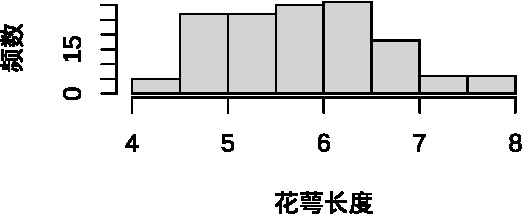
\includegraphics{sciguide_files/figure-latex/unnamed-chunk-21-1}

\begin{Shaded}
\begin{Highlighting}[]
\CommentTok{\# 二维可视化花萼长度与宽度的关系}
\FunctionTok{plot}\NormalTok{(iris}\SpecialCharTok{$}\NormalTok{Sepal.Length}\SpecialCharTok{\textasciitilde{}}\NormalTok{iris}\SpecialCharTok{$}\NormalTok{Sepal.Width,}\AttributeTok{xlab =} \StringTok{\textquotesingle{}花萼宽度\textquotesingle{}}\NormalTok{, }\AttributeTok{ylab =} \StringTok{\textquotesingle{}花萼长度\textquotesingle{}}\NormalTok{, }\AttributeTok{pch =} \DecValTok{19}\NormalTok{)}
\end{Highlighting}
\end{Shaded}

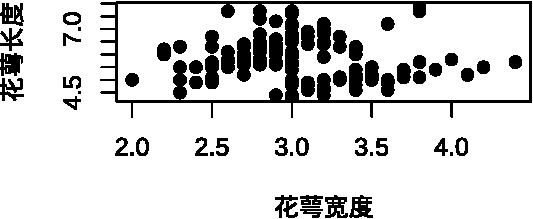
\includegraphics{sciguide_files/figure-latex/unnamed-chunk-21-2}

\begin{Shaded}
\begin{Highlighting}[]
\CommentTok{\# 三维可视化花萼长度、宽度及种属的关系}
\FunctionTok{plot}\NormalTok{(iris}\SpecialCharTok{$}\NormalTok{Sepal.Length}\SpecialCharTok{\textasciitilde{}}\NormalTok{iris}\SpecialCharTok{$}\NormalTok{Sepal.Width,}\AttributeTok{xlab =} \StringTok{\textquotesingle{}花萼宽度\textquotesingle{}}\NormalTok{, }\AttributeTok{ylab =} \StringTok{\textquotesingle{}花萼长度\textquotesingle{}}\NormalTok{, }\AttributeTok{col=}\NormalTok{ iris}\SpecialCharTok{$}\NormalTok{Species, }\AttributeTok{pch =} \FunctionTok{c}\NormalTok{(}\DecValTok{15}\NormalTok{,}\DecValTok{17}\NormalTok{,}\DecValTok{19}\NormalTok{)[}\FunctionTok{as.numeric}\NormalTok{(iris}\SpecialCharTok{$}\NormalTok{Species)])}
\FunctionTok{legend}\NormalTok{(}\StringTok{\textquotesingle{}topright\textquotesingle{}}\NormalTok{,}\AttributeTok{legend =} \FunctionTok{unique}\NormalTok{(iris}\SpecialCharTok{$}\NormalTok{Species), }\AttributeTok{col =} \FunctionTok{unique}\NormalTok{(iris}\SpecialCharTok{$}\NormalTok{Species), }\AttributeTok{pch =} \FunctionTok{c}\NormalTok{(}\DecValTok{15}\NormalTok{,}\DecValTok{17}\NormalTok{,}\DecValTok{19}\NormalTok{))}
\end{Highlighting}
\end{Shaded}

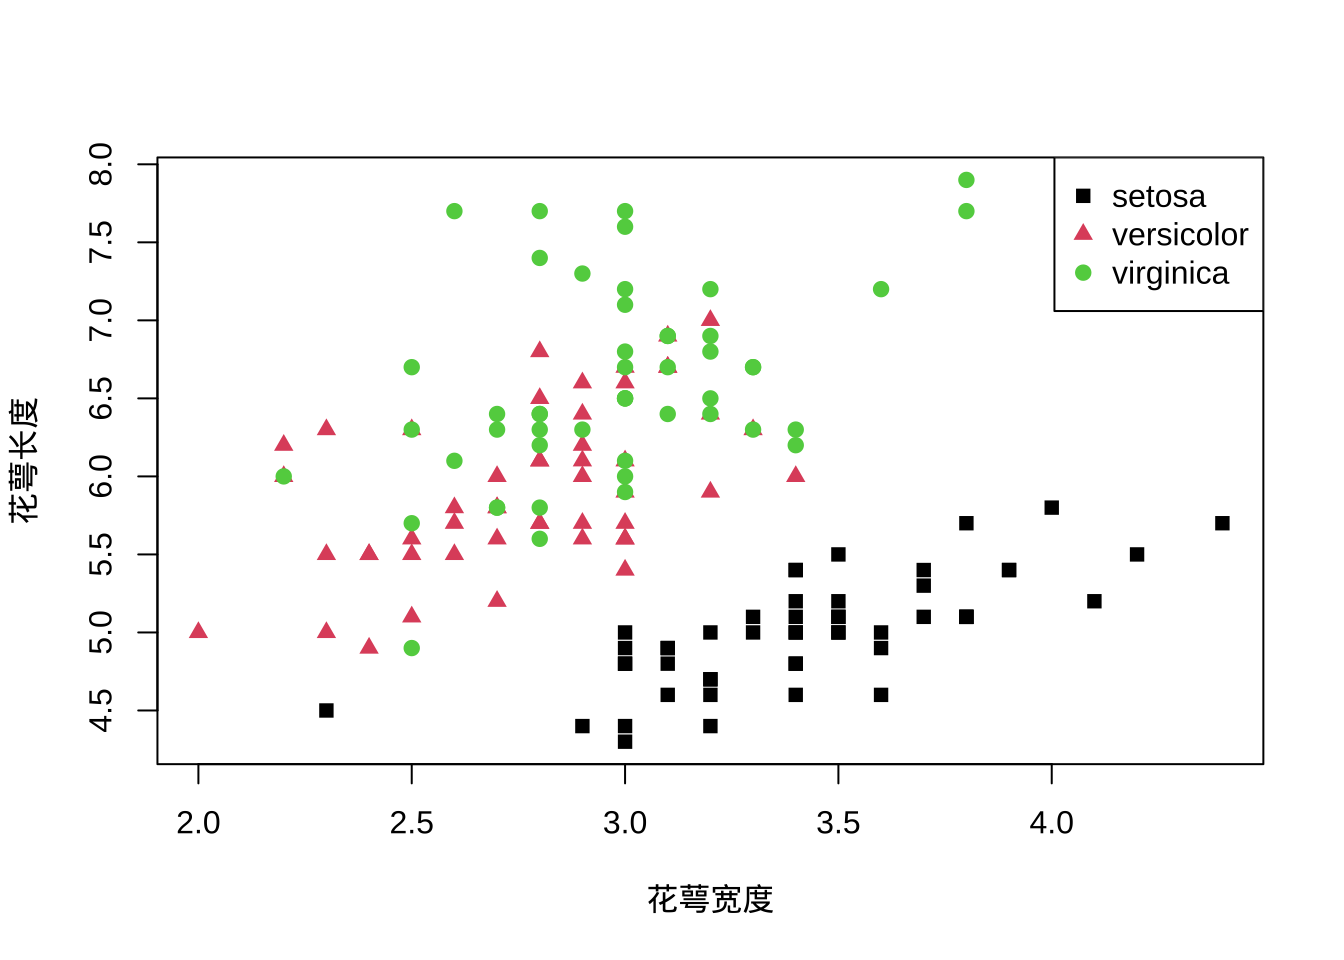
\includegraphics{sciguide_files/figure-latex/unnamed-chunk-21-3}

\begin{Shaded}
\begin{Highlighting}[]
\CommentTok{\# 利用样本相关性探索样本间关系,这里用32辆车的10维测试数据}
\NormalTok{cor }\OtherTok{\textless{}{-}} \FunctionTok{cor}\NormalTok{(}\FunctionTok{t}\NormalTok{(mtcars))}
\CommentTok{\# 相关系数阈值0.99}
\NormalTok{cor[cor}\SpecialCharTok{\textless{}}\FloatTok{0.99}\NormalTok{] }\OtherTok{\textless{}{-}} \DecValTok{0}
\NormalTok{df }\OtherTok{\textless{}{-}} \FunctionTok{data.frame}\NormalTok{(}\AttributeTok{from=}\FunctionTok{rownames}\NormalTok{(mtcars)[}\FunctionTok{which}\NormalTok{(}\FunctionTok{lower.tri}\NormalTok{(cor), }\AttributeTok{arr.ind =}\NormalTok{ T)[, }\DecValTok{1}\NormalTok{]],}\AttributeTok{to=}\FunctionTok{rownames}\NormalTok{(mtcars)[}\FunctionTok{which}\NormalTok{(}\FunctionTok{lower.tri}\NormalTok{(cor), }\AttributeTok{arr.ind =}\NormalTok{ T)[, }\DecValTok{2}\NormalTok{]],}\AttributeTok{cor=}\NormalTok{cor[}\FunctionTok{lower.tri}\NormalTok{(cor)])}
\NormalTok{df }\OtherTok{\textless{}{-}}\NormalTok{ df[}\FunctionTok{abs}\NormalTok{(df}\SpecialCharTok{$}\NormalTok{cor)}\SpecialCharTok{\textgreater{}}\DecValTok{0}\NormalTok{,]}
\CommentTok{\# 用网络可视化}
\FunctionTok{library}\NormalTok{(igraph)}
\end{Highlighting}
\end{Shaded}

\begin{verbatim}
## 
## Attaching package: 'igraph'
\end{verbatim}

\begin{verbatim}
## The following objects are masked from 'package:stats':
## 
##     decompose, spectrum
\end{verbatim}

\begin{verbatim}
## The following object is masked from 'package:base':
## 
##     union
\end{verbatim}

\begin{Shaded}
\begin{Highlighting}[]
\FunctionTok{library}\NormalTok{(ggraph)}
\end{Highlighting}
\end{Shaded}

\begin{verbatim}
## Loading required package: ggplot2
\end{verbatim}

\begin{Shaded}
\begin{Highlighting}[]
\NormalTok{net }\OtherTok{\textless{}{-}} \FunctionTok{graph\_from\_data\_frame}\NormalTok{(df,}\AttributeTok{directed =}\NormalTok{ F)}
\FunctionTok{autograph}\NormalTok{(net,}\AttributeTok{layout =} \StringTok{\textquotesingle{}fr\textquotesingle{}}\NormalTok{,}\AttributeTok{node\_size =} \DecValTok{3}\NormalTok{,)}\SpecialCharTok{+}
        \FunctionTok{geom\_node\_text}\NormalTok{(}\FunctionTok{aes}\NormalTok{(}\AttributeTok{label =}\NormalTok{ name), }\AttributeTok{repel =} \ConstantTok{TRUE}\NormalTok{, }
                 \AttributeTok{point.padding =} \FunctionTok{unit}\NormalTok{(}\FloatTok{0.2}\NormalTok{, }\StringTok{"lines"}\NormalTok{)) }\SpecialCharTok{+}
        \FunctionTok{guides}\NormalTok{(}\AttributeTok{size =} \StringTok{\textquotesingle{}none\textquotesingle{}}\NormalTok{)}\SpecialCharTok{+}
        \FunctionTok{theme\_void}\NormalTok{()}
\end{Highlighting}
\end{Shaded}

\begin{verbatim}
## Warning: ggrepel: 20 unlabeled data points (too many overlaps). Consider
## increasing max.overlaps
\end{verbatim}


\includegraphics{sciguide_files/figure-latex/unnamed-chunk-21-4}

探索性分析不同于基于假设的统计推断,往往更侧重直观展示与形成假设,后者则侧重验证与预测。探索性数据分析对于科研非常重要,因为很多新现象规律的发现都是在这阶段完成的。相应的,科研人员应掌握足够多的可视化工具,了解其探索的关系与原理,基于 R 语言可参考\href{https://bookdown.org/xiangyun/msg/}{《现代统计图形》}。

\hypertarget{ux7edfux8ba1ux63a8ux65ad}{%
\section{统计推断}\label{ux7edfux8ba1ux63a8ux65ad}}

探索性分析之后对于数据应该形成一定的感知,例如看到一些分组差异或分布趋势。此时通常要做的是统计推断,也就是判断这个差异是否真实存在。统计推断第一步是抽象出统计量,第二步是对统计量进行假设检验,这样就可以得到初步的结论。

统计量可根据探索性分析来决定,单一维度的统计量一般就是均值、方差、众数、中位数这些而多维度的统计量就涉及协方差、相关系数这类。统计量是描述总体的,可以通过对总体进行简单随机抽样获得。

这里经常混淆的概念就是标准差与标准误,其实这两个统计量描述的就不是一个东西。标准差是描述总体的,跟采样无关。也就是说,样本均值就是总体均值的无偏估计,样本的方差也是总体方差的无偏估计而标准差就是样本方差开平方。然而,标准误是衡量样本均值的变动情况,是描述样本的统计量,伴随样本数的提升,标准误会越来越小,不过此时总体的标准差是不变的。下面我们用公式来推导下这个过程,首先我们来证明样本方差是总体方差的无偏估计:

样本方差的公式是\(S^2 = \frac{\sum_{i=1}^n (X_i - \bar X)^2}{n-1}\),这里这个\(n-1\)很多人不理解,我们来计算下:

\begin{eqnarray*}
    E\left[\sum_{i=1}^n (X_i - \bar X)^2\right] & = & \sum_{i=1}^n E\left[X_i^2\right] - n E\left[\bar X^2\right] \\ \\
    & = & \sum_{i=1}^n \left\{Var(X_i) + \mu^2\right\} - n \left\{Var(\bar X) + \mu^2\right\} \\ \\
    & = & \sum_{i=1}^n \left\{\sigma^2 + \mu^2\right\} - n \left\{\sigma^2 / n + \mu^2\right\} \\ \\
    & = & n \sigma^2 + n \mu ^ 2 - \sigma^2 - n \mu^2 \\ \\
    & = & (n - 1) \sigma^2
\end{eqnarray*}

从上面的计算中我们不但可以知道样本方差公式里为什么有个\(n-1\),也明白了为什么是总体方差的无偏估计。然后我们计算下样本均值的方差:

\begin{eqnarray*}
    Var(\bar X) & = & Var \left( \frac{1}{n}\sum_{i=1}^n X_i \right)\\ \\
    & = & \frac{1}{n^2} Var\left(\sum_{i=1}^n X_i \right)\\ \\
    & = & \frac{1}{n^2} \sum_{i=1}^n Var(X_i) \\ \\
    & = & \frac{1}{n^2} \times n\sigma^2 \\ \\
    & = & \frac{\sigma^2}{n}
\end{eqnarray*}

这里我们可以看到,样本均值的方差是跟样本数有关的而公式里总体方差可以用样本方差公式来估计,是个常量,这样就可以知道样本均值的标准差(也就是标准误)会伴随样本数增加而减小。也可以理解为我们抽样越多对均值的估计就越准,但总体方差是总体属性,不会因为我们更多的抽样而发生变化。

统计量可以是一个数值,也可以是一个区间,因此对于统计量的估计也有点估计与区间估计两种方法。现在越来越多的研究要求报告区间估计,这里只介绍下置信区间。所谓置信区间,是指在一定置信水平(通常是95\%)下包含真值的区间,是对总体参数的估计。这里一个经常出现的误解是认为95\%置信区间指真值出现在区间内的概率是95\%,这个描述的问题在于没搞清楚置信区间描述的是一个真值而不是概率,真值是唯一的,置信水平是区间内包含真值的概率。也就是说,假如我们从总体里抽样来估计均值的置信区间,这个行为重复100次,会产生100个置信区间,其中会有约95个区间内是包含真值的。这是频率学派对置信区间的解释,贝叶斯学派的可信区间是更符合真值出现在区间内的概率这个解释的,这两个学派对于数据的假设不一样,因此计算方法也不一样。

有了统计量,我们就可以进行比较了。这就是前面章节提到的NHST与p值问题,这里的问题这边不再复述,这里更多分析下一些统计推断中的概念。所谓推断,更多是要涉及决策的需要明确零假设、备择假设与p值。在这里要明确统计差异显著并不代的实际差异显著,甚至都不一定有实际意义,我们在论文里看到差异显著的描述只能说通过了统计推断里的假设检验,只是一个参考。打个比方,衣服的尺码里L码与M码差异显著,但对于一个体形介于两者之间的人而言,这两件衣服穿着都算舒服,此时究竟差异显著与否意义就不大了。

科研里最常用的比较是两独立样本均值比较的t检验与评价单因素多水平影响的方差分析。t检验可以看作方差分析的特例,使用统计量t来比较而方差分析通常是用分类变量所解释的变异比上分类变量以外的变异去进行F检验。换句话讲,如果分类变量可以解释大部分响应变量的变异,我们就说这种分类变量对响应变量的解释有意义。例如下面这组数据:

\begin{quote}
1, 1, 1, 1, 1, 2, 2, 2, 2, 2, 3, 3, 3, 3, 3
\end{quote}

总变异为10, 如果我们分组为按照相同的数放到一起,那么组内变异就是0,组间变异为10,这时我们就说这种分组有效的解释了响应变量,F值趋向正无穷。如果我们完全随机分组,组内与组间的变异差不多,那么这种分类方法并不解释响应变量,反映到F值上就是1。

但是仅仅知道是否受影响是不够的,如同上面的例子,我们知道的仅仅是存在一种分类方法可以解释响应的全部变化,其内部也是均匀的,但不同分类水平间的差异我们并不知道,这就需要多重比较了。例如,当我们对两组数据做置信度0.05的t检验,我们遇到假阳性的概率为5\%。但如果面对多组数据例如3组,进行两两比较的话就有\(3\choose2\)也就是3组对比,那么我们遇到假阳性的概率就为\(1-(1-0.05)^3\),也就是14.3\%,远高于0.05的置信度。组越多,两两对比就越多,整体上假阳性的概率就越来越大,到最后就是两组数据去对比,无论如何你都会检验出差异。

此外就方向而样,虽然我们都不承认零假设(要不然还做什么实验),但当我们默认设定为双尾检验时,假阳性就被默认发生在两个方向上了,这样的多重比较必然导致在其中一个方向上的错误率被夸大了。就影响大小而言,如果我们每次重复都选择效应最强的那一组,重复越多,预设的偏态就越重,换言之,我们的零假设因为重复实验的选择偏好而发生了改变。

那么多重比较如何应对这个问题呢?有两种思路,一种思路是我依旧采取两两对比,进行t检验,但p值的选取方法要修改,例如Bonferroni方法中就把p的阈值调整为进行多重比较的次数乘以计算得到的p值。如果我们关心的因素为2,那么计算得到的p值都要乘2来跟0.05或0.01的边界置信度进行比较;另一种思路则是修改两两比较所用的统计量,给出一个更保守的分布,那么得到p值就会更大。不论怎样,我们这样做都是为了降低假阳性,但同时功效不可避免的降低了。

多重比较的方法类型包括单步法与逐步法。单步法只考虑对零假设的影响而不考虑其他影响而逐步法则会考虑其他假设检验对单一检验的影响,例如可以先按不同分组均值差异从大到小排序,先对比第一个,有差异对比下一个,当出现无差异时停止对比;或者从下到大排序,有差异时停止对比,之后均认为有差异。此时还要注意一种特殊情况,因为F检验是从方差角度来考虑影响显著性与否,所以可能存在F检验显著但组间均值差异均不显著的情况,此时要考虑均值间线性组合的新均值的差异性。不过,大多数情况我们只用考虑不同组间两两差异比较即可。

具体而言,单步法等方差多重比较最常见的是Tukey's HSD方法,这是一个两两比较的方法,基于 studentized range 分布计算出q统计量,然后基于这个统计量进行两两间差异的假设检验。该方法适用于分组间等方差等数目的场景,如果分组内数目不同,需要用 Tukey-Kranmer 方法。该方法适用于两两比较,在分组数目相同时统计功效等同于从大到小排序的逐步法。

此外,还有些多重比较的方法在特定学科里也很常见。从总体控制错误率的角度,如果是两两比较应该选 Tukey's HSD方法;如果侧重组间差异线性组合的均值用 Scheffe test;如果对比数指定了,功效按 Gabriel、GT2、DST、 Bonferroni顺序来选;如果是各分组都跟控制组比,应该选Dunnett法;如果各分组方差不相等,用GH,C,T3等方法。此外,如果打算保证每个比较中的置信水平,应该选 Tukey、 Scheffe、Dunnett法。

与多重比较类似的一个统计推断问题是多重检验问题。多重检验指的是同时进行多次假设检验的场景,其实多重比较可以看作多重检验在方差分析里的一个特例。举例而言,我对两组样品(暴露组跟对照组)中每一个样品测定了10000个指标,每组有10个样品,那么如果我想知道差异有多大就需要对比10000次,具体说就是10000次双样本t检验。那么如果我对t检验的置信水平设置在95\%,也就是5\%假阳性,做完这10000次检验,我会期望看到500个假阳性,而这500个有显著差异的指标其实对分组不敏感也可以随机生成。假如真实测到了600个有显著差异的指标,那么如何区分其中哪些是对分组敏感?哪些又仅仅只是随机的呢?随机的会不会只有500个整呢?这个场景在组学技术与传感器技术采集高通量高维数据的今天变得越来越普遍。

这个问题在做经典科研实验时往往会忽略,深层次的原因是经典的科研实验往往是理论或经验主导需要进行检验的假说。例如,我测定血液中白血球的数目就可以知道你是不是处于炎症中,其背后是医学知识的支撑。然而,在组学或其他高通量实验中,研究实际是数据导向的,也就是不管有用没用反正我测了一堆指标,然后就去对比差异,然后就是上面的问题了,我们可能分不清楚哪些是真的相关,哪些又是随机出现的。

对于单次比较,当我们看到显著差异的p值脑子里想的是零假设为真时发生的概率,当我们置信水平设定在0.95而p值低于对应的阈值,那么我们应该拒绝零假设。但对比次数多了从概率上就会出现已经被拒绝的假设实际是错误的而你不知道是哪一个。整体错误率控制的思路就是我不管单次比较了,我只对你这所有的对比次数的总错误率进行控制。还是上面的例子,对于10000次假设检验我只能接受1个错误,整体犯错概率为0.0001,那么对于单次比较,其假阳性也得设定在这个水平上去进行假设检验,结果整体上错误率是控制住了,但对于单次比较就显得十分严格了。下面用一个仿真实验来说明:

\begin{Shaded}
\begin{Highlighting}[]
\FunctionTok{set.seed}\NormalTok{(}\DecValTok{42}\NormalTok{)}
\CommentTok{\# 随机数的10000次比较}
\NormalTok{pvalue }\OtherTok{\textless{}{-}} \ConstantTok{NULL}
\ControlFlowTok{for}\NormalTok{ (i }\ControlFlowTok{in} \DecValTok{1}\SpecialCharTok{:}\DecValTok{10000}\NormalTok{) \{}
\NormalTok{  a }\OtherTok{\textless{}{-}} \FunctionTok{rnorm}\NormalTok{(}\DecValTok{10}\NormalTok{)}
\NormalTok{  b }\OtherTok{\textless{}{-}} \FunctionTok{rnorm}\NormalTok{(}\DecValTok{10}\NormalTok{)}
\NormalTok{  c }\OtherTok{\textless{}{-}} \FunctionTok{t.test}\NormalTok{(a, b)}
\NormalTok{  pvalue[i] }\OtherTok{\textless{}{-}}\NormalTok{ c}\SpecialCharTok{$}\NormalTok{p.value}
\NormalTok{\}}
\CommentTok{\# 看下p值分布}
\FunctionTok{hist}\NormalTok{(}
\NormalTok{  pvalue,}
  \AttributeTok{main =} \FunctionTok{substitute}\NormalTok{(}\FunctionTok{paste}\NormalTok{(}\FunctionTok{italic}\NormalTok{(}\StringTok{\textquotesingle{}p\textquotesingle{}}\NormalTok{), }\StringTok{"值分布"}\NormalTok{)),}
  \AttributeTok{xlab =} \FunctionTok{substitute}\NormalTok{(}\FunctionTok{paste}\NormalTok{(}\FunctionTok{italic}\NormalTok{(}\StringTok{\textquotesingle{}p\textquotesingle{}}\NormalTok{), }\StringTok{"值"}\NormalTok{)),}
  \AttributeTok{ylab =} \StringTok{\textquotesingle{}频率\textquotesingle{}}
\NormalTok{)}
\end{Highlighting}
\end{Shaded}

\begin{figure}
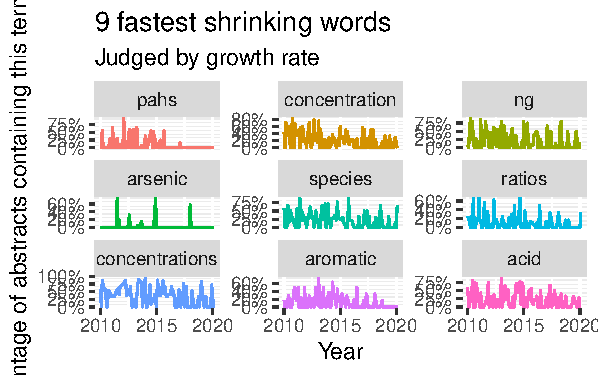
\includegraphics{sciguide_files/figure-latex/unnamed-chunk-22-1} \caption[随机数进行t检验后p值分布]{随机数进行t检验后p值分布}\label{fig:unnamed-chunk-22}
\end{figure}

\begin{Shaded}
\begin{Highlighting}[]
\CommentTok{\# 小于0.05的个数}
\FunctionTok{sum}\NormalTok{(pvalue }\SpecialCharTok{\textless{}} \FloatTok{0.05}\NormalTok{)}
\end{Highlighting}
\end{Shaded}

\begin{verbatim}
## [1] 477
\end{verbatim}

\begin{Shaded}
\begin{Highlighting}[]
\CommentTok{\# 小于0.0001的个数}
\FunctionTok{sum}\NormalTok{(pvalue }\SpecialCharTok{\textless{}} \FloatTok{0.0001}\NormalTok{)}
\end{Highlighting}
\end{Shaded}

\begin{verbatim}
## [1] 0
\end{verbatim}

这样我们会看到进行了整体的控制之后,确实是找不到有差异的了,而且此时我们也可以看到p值的分布应该是0到1之间的均匀分布。但假如里面本来就有有差异的呢?

\begin{Shaded}
\begin{Highlighting}[]
\FunctionTok{set.seed}\NormalTok{(}\DecValTok{42}\NormalTok{)}
\NormalTok{pvalue }\OtherTok{\textless{}{-}} \ConstantTok{NULL}
\ControlFlowTok{for}\NormalTok{ (i }\ControlFlowTok{in} \DecValTok{1}\SpecialCharTok{:}\DecValTok{10000}\NormalTok{) \{}
\NormalTok{  a }\OtherTok{\textless{}{-}} \FunctionTok{rnorm}\NormalTok{(}\DecValTok{10}\NormalTok{, }\DecValTok{1}\NormalTok{)}
\NormalTok{  b }\OtherTok{\textless{}{-}}\NormalTok{ a }\SpecialCharTok{+} \DecValTok{1}
\NormalTok{  c }\OtherTok{\textless{}{-}} \FunctionTok{t.test}\NormalTok{(a, b)}
\NormalTok{  pvalue[i] }\OtherTok{\textless{}{-}}\NormalTok{ c}\SpecialCharTok{$}\NormalTok{p.value}
\NormalTok{\}}
\CommentTok{\# 看下p值分布}
\FunctionTok{hist}\NormalTok{(}
\NormalTok{  pvalue,}
  \AttributeTok{main =} \FunctionTok{substitute}\NormalTok{(}\FunctionTok{paste}\NormalTok{(}\FunctionTok{italic}\NormalTok{(}\StringTok{\textquotesingle{}p\textquotesingle{}}\NormalTok{), }\StringTok{"值分布"}\NormalTok{)),}
  \AttributeTok{xlab =} \FunctionTok{substitute}\NormalTok{(}\FunctionTok{paste}\NormalTok{(}\FunctionTok{italic}\NormalTok{(}\StringTok{\textquotesingle{}p\textquotesingle{}}\NormalTok{), }\StringTok{"值"}\NormalTok{)),}
  \AttributeTok{ylab =} \StringTok{\textquotesingle{}频率\textquotesingle{}}
\NormalTok{)}
\end{Highlighting}
\end{Shaded}

\begin{figure}
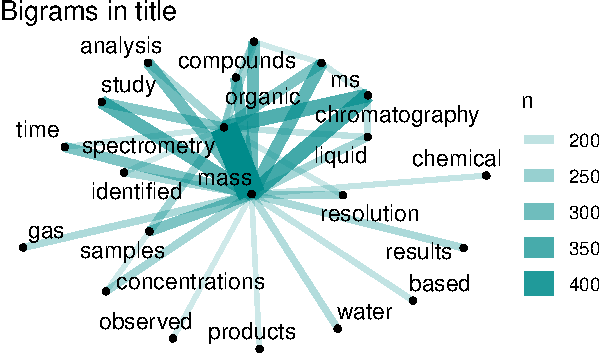
\includegraphics{sciguide_files/figure-latex/unnamed-chunk-23-1} \caption[存在真实差异时p值的分布]{存在真实差异时p值的分布}\label{fig:unnamed-chunk-23}
\end{figure}

\begin{Shaded}
\begin{Highlighting}[]
\CommentTok{\# 显示p值里小于0.05的个数}
\FunctionTok{sum}\NormalTok{(pvalue }\SpecialCharTok{\textless{}} \FloatTok{0.05}\NormalTok{)}
\end{Highlighting}
\end{Shaded}

\begin{verbatim}
## [1] 6559
\end{verbatim}

\begin{Shaded}
\begin{Highlighting}[]
\CommentTok{\# 显示p值里小于0.0001的个数}
\FunctionTok{sum}\NormalTok{(pvalue }\SpecialCharTok{\textless{}} \FloatTok{0.0001}\NormalTok{)}
\end{Highlighting}
\end{Shaded}

\begin{verbatim}
## [1] 45
\end{verbatim}

上面我们模拟了10000次有真实差异的假设检验,结果按照单次检验0.05的阈值能发现约7000有差异,而使用0.0001却只能发现不到100次有显著差异。那么问题很明显,或许控制整体错误率可以让我们远离假阳性,但假阴性就大幅提高了或者说功效降低了,最后的结果可能是什么差异也看不到。

下面我们尝试一个更切合实际的模拟,混合有差异跟无差异的检验:

\begin{Shaded}
\begin{Highlighting}[]
\FunctionTok{set.seed}\NormalTok{(}\DecValTok{42}\NormalTok{)}
\NormalTok{pvalue }\OtherTok{\textless{}{-}} \ConstantTok{NULL}
\ControlFlowTok{for}\NormalTok{ (i }\ControlFlowTok{in} \DecValTok{1}\SpecialCharTok{:}\DecValTok{5000}\NormalTok{) \{}
\NormalTok{  a }\OtherTok{\textless{}{-}} \FunctionTok{rnorm}\NormalTok{(}\DecValTok{10}\NormalTok{, }\DecValTok{1}\NormalTok{)}
\NormalTok{  b }\OtherTok{\textless{}{-}}\NormalTok{ a }\SpecialCharTok{+} \DecValTok{1}
\NormalTok{  c }\OtherTok{\textless{}{-}} \FunctionTok{t.test}\NormalTok{(a, b)}
\NormalTok{  pvalue[i] }\OtherTok{\textless{}{-}}\NormalTok{ c}\SpecialCharTok{$}\NormalTok{p.value}
\NormalTok{\}}
\ControlFlowTok{for}\NormalTok{ (i }\ControlFlowTok{in} \DecValTok{1}\SpecialCharTok{:}\DecValTok{5000}\NormalTok{) \{}
\NormalTok{  a }\OtherTok{\textless{}{-}} \FunctionTok{rnorm}\NormalTok{(}\DecValTok{10}\NormalTok{, }\DecValTok{1}\NormalTok{)}
\NormalTok{  b }\OtherTok{\textless{}{-}} \FunctionTok{rnorm}\NormalTok{(}\DecValTok{10}\NormalTok{, }\DecValTok{1}\NormalTok{)}
\NormalTok{  c }\OtherTok{\textless{}{-}} \FunctionTok{t.test}\NormalTok{(a, b)}
\NormalTok{  pvalue[i }\SpecialCharTok{+} \DecValTok{5000}\NormalTok{] }\OtherTok{\textless{}{-}}\NormalTok{ c}\SpecialCharTok{$}\NormalTok{p.value}
\NormalTok{\}}
\CommentTok{\# 看下p值分布}
\FunctionTok{hist}\NormalTok{(}
\NormalTok{  pvalue,}
  \AttributeTok{main =} \FunctionTok{substitute}\NormalTok{(}\FunctionTok{paste}\NormalTok{(}\FunctionTok{italic}\NormalTok{(}\StringTok{\textquotesingle{}p\textquotesingle{}}\NormalTok{), }\StringTok{"值分布"}\NormalTok{)),}
  \AttributeTok{xlab =} \FunctionTok{substitute}\NormalTok{(}\FunctionTok{paste}\NormalTok{(}\FunctionTok{italic}\NormalTok{(}\StringTok{\textquotesingle{}p\textquotesingle{}}\NormalTok{), }\StringTok{"值"}\NormalTok{)),}
  \AttributeTok{ylab =} \StringTok{\textquotesingle{}频率\textquotesingle{}}
\NormalTok{)}
\end{Highlighting}
\end{Shaded}

\begin{figure}
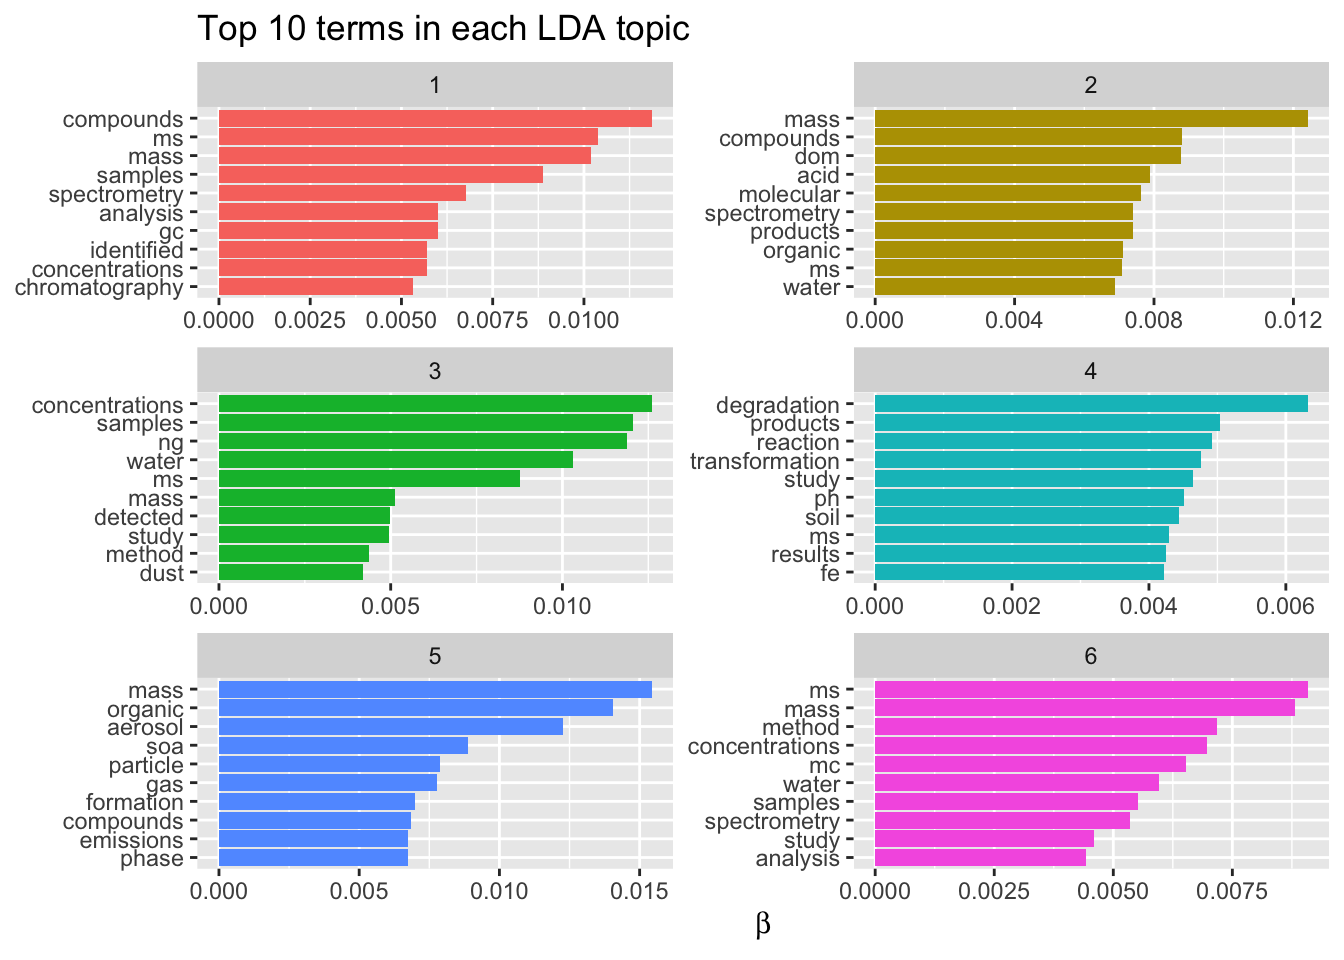
\includegraphics{sciguide_files/figure-latex/unnamed-chunk-24-1} \caption[混合有差异与无差异的检验时p值的分布]{混合有差异与无差异的检验时p值的分布}\label{fig:unnamed-chunk-24}
\end{figure}

\begin{Shaded}
\begin{Highlighting}[]
\CommentTok{\# 显示p值里小于0.05的个数}
\FunctionTok{sum}\NormalTok{(pvalue }\SpecialCharTok{\textless{}} \FloatTok{0.05}\NormalTok{)}
\end{Highlighting}
\end{Shaded}

\begin{verbatim}
## [1] 3499
\end{verbatim}

\begin{Shaded}
\begin{Highlighting}[]
\CommentTok{\# 显示p值里小于0.0001的个数}
\FunctionTok{sum}\NormalTok{(pvalue }\SpecialCharTok{\textless{}} \FloatTok{0.0001}\NormalTok{)}
\end{Highlighting}
\end{Shaded}

\begin{verbatim}
## [1] 21
\end{verbatim}

此时结果就更有意思了,明明应该有5000次是有差异的,但阈值设定在0.05只能看到约3500次,而0.0001只能看到24次。

上面的模拟告诉我们,降低假阳性的方法会提高假阴性的比率,也就是功效不足,无法发现本来就有的差异。而且似乎本来0.05的阈值对于真阳性也是偏小的。同时,面对假设检验概率低于0.05的那些差异,我们也没有很好的方法区别哪些是真的,哪些是随机的。其实很多人都知道整体错误率控制是比较严格的,会损失统计功效。但也不是完全没人用,例如寻找生物标记物做重大疾病诊断时就不太能接受假阳性而可以接受一定的假阴性,此时如果标准放宽就会找到一大堆假信号,到时候标记不准就会对诊断产生负面影响。

下面介绍下常见的两种整体错误率控制方法。第一种是 Bonferroni 方法,控制的是整体错误率(FWER),思路很简单,就是控制显著性,例如单次检验假阳性比率\(\alpha\)控制在0.05,那么n次检验假阳性比率控制为\(\frac{\alpha}{n}\)。这样实际是对整体采用了个体控制的控制思路:

\[
P(至少一个显著)=1-P(无显著差异) = 1-(1-\alpha/n)^n
\]

我们来看下\(\alpha = 0.05\)随比较数增加的效果:

\begin{Shaded}
\begin{Highlighting}[]
\CommentTok{\# 比较次数}
\NormalTok{n }\OtherTok{\textless{}{-}} \FunctionTok{c}\NormalTok{(}\DecValTok{1}\SpecialCharTok{:}\DecValTok{10} \SpecialCharTok{\%o\%} \DecValTok{10} \SpecialCharTok{\^{}}\NormalTok{ (}\DecValTok{1}\SpecialCharTok{:}\DecValTok{2}\NormalTok{))}
\CommentTok{\# 整体出现假阳性概率}
\NormalTok{p0 }\OtherTok{\textless{}{-}} \DecValTok{1} \SpecialCharTok{{-}}\NormalTok{ (}\DecValTok{1} \SpecialCharTok{{-}} \FloatTok{0.05}\NormalTok{) }\SpecialCharTok{\^{}}\NormalTok{ n}
\CommentTok{\# Bonferroni方法控制后的整体假阳性概率}
\NormalTok{p }\OtherTok{\textless{}{-}} \DecValTok{1} \SpecialCharTok{{-}}\NormalTok{ (}\DecValTok{1} \SpecialCharTok{{-}} \FloatTok{0.05} \SpecialCharTok{/}\NormalTok{ n) }\SpecialCharTok{\^{}}\NormalTok{ n}
\CommentTok{\# 不进行控制}
\FunctionTok{plot}\NormalTok{(}
\NormalTok{  p0 }\SpecialCharTok{\textasciitilde{}}\NormalTok{ n,}
  \AttributeTok{ylim =} \FunctionTok{c}\NormalTok{(}\DecValTok{0}\NormalTok{, }\DecValTok{1}\NormalTok{),}
  \AttributeTok{pch =} \DecValTok{19}\NormalTok{,}
  \AttributeTok{xlab =} \StringTok{\textquotesingle{}测试数\textquotesingle{}}\NormalTok{,}
  \AttributeTok{ylab =} \StringTok{\textquotesingle{}整体错误率(FWER)\textquotesingle{}}
\NormalTok{)}
\CommentTok{\# Bonferroni方法控制}
\FunctionTok{points}\NormalTok{(p }\SpecialCharTok{\textasciitilde{}}\NormalTok{ n, }\AttributeTok{pch =} \DecValTok{17}\NormalTok{, }\AttributeTok{col =} \StringTok{\textquotesingle{}grey\textquotesingle{}}\NormalTok{)}
\FunctionTok{legend}\NormalTok{(}\StringTok{\textquotesingle{}right\textquotesingle{}}\NormalTok{,}
       \FunctionTok{c}\NormalTok{(}\StringTok{\textquotesingle{}Bonferroni方法\textquotesingle{}}\NormalTok{, }\StringTok{\textquotesingle{}无矫正\textquotesingle{}}\NormalTok{),}
       \AttributeTok{pch =} \FunctionTok{c}\NormalTok{(}\DecValTok{17}\NormalTok{,}\DecValTok{19}\NormalTok{),}
       \AttributeTok{col =} \FunctionTok{c}\NormalTok{(}\StringTok{\textquotesingle{}grey\textquotesingle{}}\NormalTok{,}\StringTok{\textquotesingle{}black\textquotesingle{}}\NormalTok{))}
\end{Highlighting}
\end{Shaded}

\begin{figure}
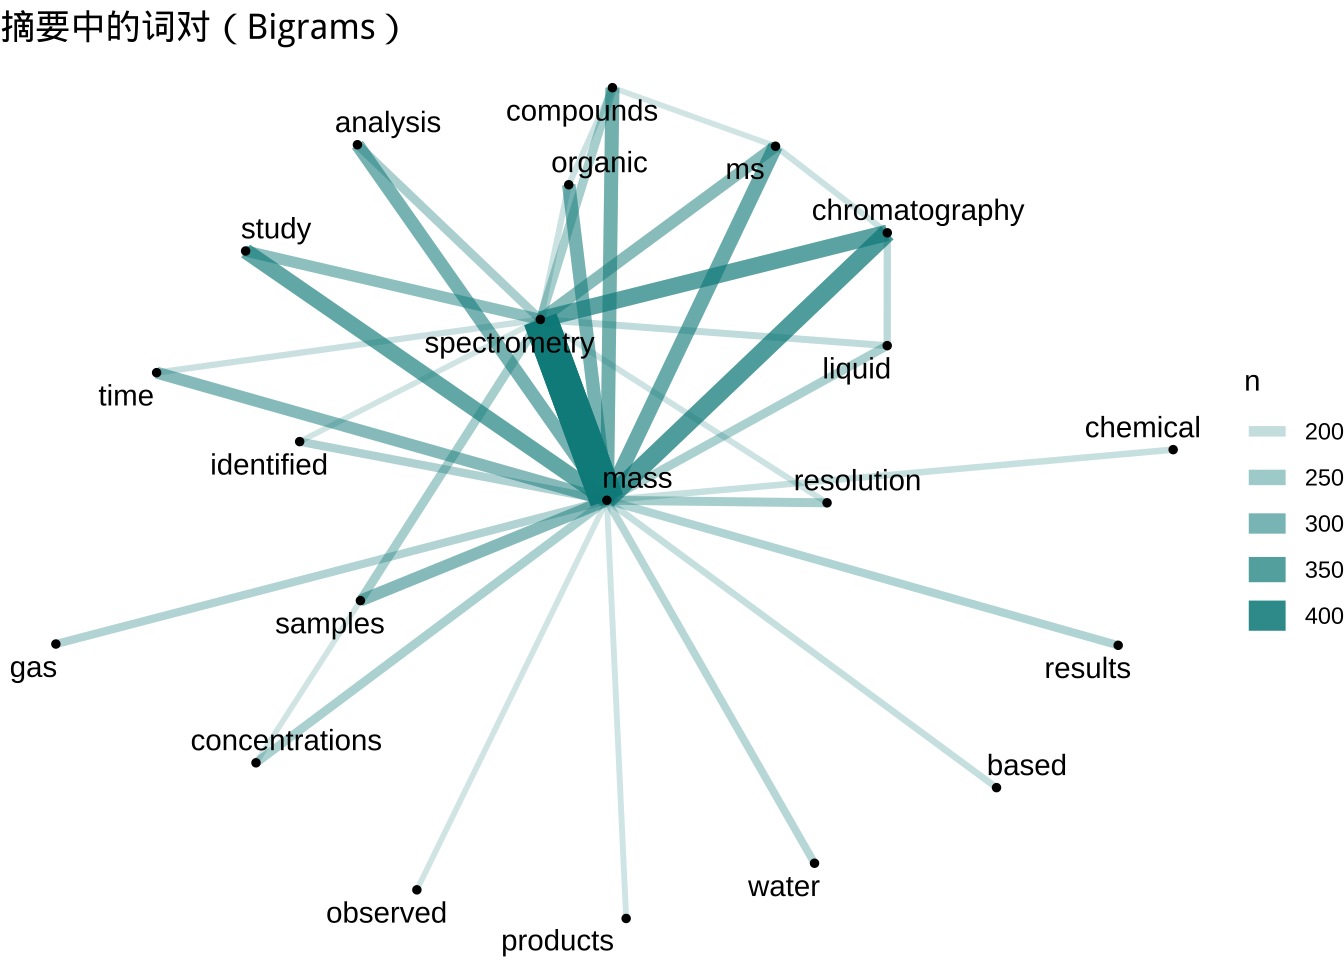
\includegraphics{sciguide_files/figure-latex/unnamed-chunk-25-1} \caption[对比Bonferroni方法与无矫正时整体错误率的变化]{对比Bonferroni方法与无矫正时整体错误率的变化}\label{fig:unnamed-chunk-25}
\end{figure}

其实,这样的控制得到的整体错误率是略低于0.05的,并且数目越大,整体错误率越低。这个方法十分保守,有可能什么差异你都看不到,因为都变成假阴性了。在实际应用中一般不调节p值的假阳性比率而直接调节p值,取原始p值跟整体检验数目的乘积与1的最小值作为调节p值,还可以用0.05或0.01进行判断,不过这时候控制的整体而不是单一检验了。

当然这只是最原始的 Bonferroni 方法,后来Holm改进了这种一步法为逐步法,此时我们需要首先对原始p值进行排序,然后每个原始p值乘上其排序作为调节p值。例如三次多重检验的p值分别是0.01、0.03与0.06,排序为3、2、1,其调节后的p值为0.03,0.06,0.06。如果我们控制整体假阳性比率低于0.05,那么调解后只有第一个检验可以拒绝零假设。值得注意的是Holm的改进是全面优于原始方法的,也就是说当你一定要去用Bonferroni方法控制整体错误率,优先选Holm的改进版。

上面那种方法其实有点非参的意思,其实数学上我们是可以精确的把假阳性比率控制在某个数值的,也就是Sidak方法:

\[
P(至少一个显著)=1-P(无显著差异) = 1-(1-\alpha')^n = 0.05
\]

求解可得到\(\alpha' = 1-0.95^{\frac{1}{n}}\),此时我们就可以比较精确的控制整体错误率了,但是,这个方法有个前提就是各个检验必须是独立的,这在生物学实验里几乎不可能,所以这个方法的应用远没有Bonferroni方法广。

刚才的模拟中我们可以看到,控制整体错误率比较严格,假阴性比率高,那么有没有办法找到假阴性比率低或者说功效高的呢?要知道我们其实只关心有差异的那部分中那些是真的,哪些是假的,无差异的可以完全不用考虑。那么我们可以尝试控制错误发现率(FDR),也就是在有差异的那一部分指标中控制错误率低于某一水平。

\begin{Shaded}
\begin{Highlighting}[]
\CommentTok{\# 所有有差异的}
\NormalTok{R }\OtherTok{\textless{}{-}} \FunctionTok{sum}\NormalTok{(pvalue}\SpecialCharTok{\textless{}}\FloatTok{0.05}\NormalTok{)}
\NormalTok{R}
\end{Highlighting}
\end{Shaded}

\begin{verbatim}
## [1] 3499
\end{verbatim}

\begin{Shaded}
\begin{Highlighting}[]
\CommentTok{\# 假阳性}
\NormalTok{V }\OtherTok{\textless{}{-}} \FunctionTok{sum}\NormalTok{(pvalue[}\DecValTok{5001}\SpecialCharTok{:}\DecValTok{10000}\NormalTok{]}\SpecialCharTok{\textless{}}\FloatTok{0.05}\NormalTok{)}
\NormalTok{V}
\end{Highlighting}
\end{Shaded}

\begin{verbatim}
## [1] 225
\end{verbatim}

\begin{Shaded}
\begin{Highlighting}[]
\CommentTok{\# 错误发现率}
\NormalTok{Q }\OtherTok{\textless{}{-}}\NormalTok{ V}\SpecialCharTok{/}\NormalTok{R}
\NormalTok{Q}
\end{Highlighting}
\end{Shaded}

\begin{verbatim}
## [1] 0.06430409
\end{verbatim}

上面的计算显示虽然我们漏掉了很多阳性结果,但错误发现率并不高。事实上如果我们控制错误率到0.01,错误发现率会更低:

\begin{Shaded}
\begin{Highlighting}[]
\CommentTok{\# 所有有差异的}
\NormalTok{R }\OtherTok{\textless{}{-}} \FunctionTok{sum}\NormalTok{(pvalue}\SpecialCharTok{\textless{}}\FloatTok{0.01}\NormalTok{)}
\NormalTok{R}
\end{Highlighting}
\end{Shaded}

\begin{verbatim}
## [1] 999
\end{verbatim}

\begin{Shaded}
\begin{Highlighting}[]
\CommentTok{\# 假阳性}
\NormalTok{V }\OtherTok{\textless{}{-}} \FunctionTok{sum}\NormalTok{(pvalue[}\DecValTok{5001}\SpecialCharTok{:}\DecValTok{10000}\NormalTok{]}\SpecialCharTok{\textless{}}\FloatTok{0.01}\NormalTok{)}
\NormalTok{V}
\end{Highlighting}
\end{Shaded}

\begin{verbatim}
## [1] 34
\end{verbatim}

\begin{Shaded}
\begin{Highlighting}[]
\CommentTok{\# 错误发现率}
\NormalTok{Q }\OtherTok{\textless{}{-}}\NormalTok{ V}\SpecialCharTok{/}\NormalTok{R}
\NormalTok{Q}
\end{Highlighting}
\end{Shaded}

\begin{verbatim}
## [1] 0.03403403
\end{verbatim}

其实出现这个问题不难理解,零假设检验里p值是均匀分布的而有差异检验的p值是有偏分布且偏向于较小的数值,所以假阳性控制的越小,有偏分布占比例就越高,但同时会造成假阴性提高的问题。

那么错误发现率会不会比整体错误率的控制更好呢?这里通过两种常见的控制方法进行说明。

Benjamini-Hochberg方法跟Holm方法很像,也是先排序,但之后p值并不是简单的乘排序,而是乘检验总数后除排序:

\[
p_i \leq \frac{i}{m} \alpha
\]

举例来说就是假设三次多重检验的p值分别是0.01、0.03与0.06,其调节后的p值为0.03,0.45,0.06。那么为什么说这种方法控制的是错误发现率呢?我们来看下\(\alpha\)是如何得到的:p值乘总数m得到的是在该p值下理论发现数,而除以其排序实际是该p值下实际发现数,理论发现数基于在这里的分布是均匀分布,也就是零假设的分布,这两个的比值自然就是错误发现率。下面我用仿真实验来说明一下:

\begin{Shaded}
\begin{Highlighting}[]
\CommentTok{\# BH法控制错误发现率}
\NormalTok{pbh }\OtherTok{\textless{}{-}} \FunctionTok{p.adjust}\NormalTok{(pvalue, }\AttributeTok{method =} \StringTok{\textquotesingle{}BH\textquotesingle{}}\NormalTok{)}
\CommentTok{\# holm法控制错误发现率}
\NormalTok{ph }\OtherTok{\textless{}{-}} \FunctionTok{p.adjust}\NormalTok{(pvalue, }\AttributeTok{method =} \StringTok{\textquotesingle{}holm\textquotesingle{}}\NormalTok{)}
\FunctionTok{plot}\NormalTok{(pbh }\SpecialCharTok{\textasciitilde{}}\NormalTok{ pvalue,}
     \AttributeTok{ylab =} \StringTok{\textquotesingle{}错误发现率(FDR)\textquotesingle{}}\NormalTok{,}
     \AttributeTok{xlab =} \FunctionTok{substitute}\NormalTok{(}\FunctionTok{paste}\NormalTok{(}\FunctionTok{italic}\NormalTok{(}\StringTok{\textquotesingle{}p\textquotesingle{}}\NormalTok{), }\StringTok{"值"}\NormalTok{)),}
     \AttributeTok{pch =} \DecValTok{19}\NormalTok{)}
\FunctionTok{points}\NormalTok{(ph }\SpecialCharTok{\textasciitilde{}}\NormalTok{ pvalue, }\AttributeTok{pch =} \DecValTok{17}\NormalTok{, }\AttributeTok{col =} \StringTok{\textquotesingle{}grey\textquotesingle{}}\NormalTok{)}
\FunctionTok{legend}\NormalTok{(}\StringTok{\textquotesingle{}bottomright\textquotesingle{}}\NormalTok{,}
       \FunctionTok{c}\NormalTok{(}\StringTok{\textquotesingle{}Holm 法\textquotesingle{}}\NormalTok{, }\StringTok{\textquotesingle{}BH 法\textquotesingle{}}\NormalTok{),}
       \AttributeTok{col =} \FunctionTok{c}\NormalTok{(}\StringTok{\textquotesingle{}grey\textquotesingle{}}\NormalTok{, }\StringTok{\textquotesingle{}black\textquotesingle{}}\NormalTok{),}
       \AttributeTok{pch =} \FunctionTok{c}\NormalTok{(}\DecValTok{17}\NormalTok{,}\DecValTok{19}\NormalTok{))}
\end{Highlighting}
\end{Shaded}

\begin{figure}
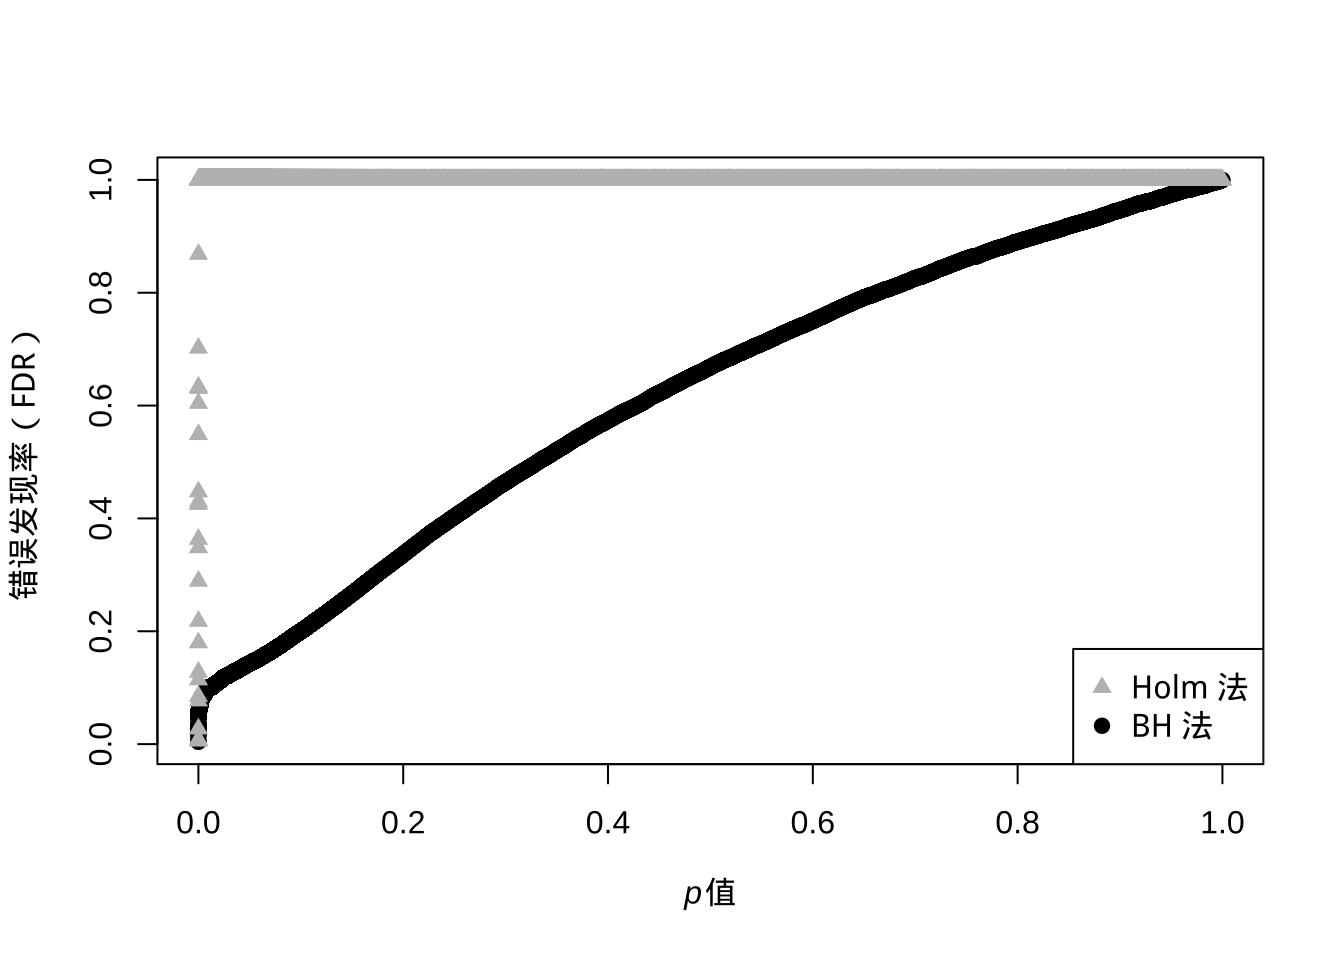
\includegraphics{sciguide_files/figure-latex/unnamed-chunk-28-1} \caption[p值的Holm 法与 BH 法与控制错误发现率的变化]{p值的Holm 法与 BH 法与控制错误发现率的变化}\label{fig:unnamed-chunk-28}
\end{figure}

从上面图我们可以看出,如果控制整体错误率(浅色),那么p值很容易就到1了,过于严格。而如果用BH方法控制错误发现率,那么原始p值越大,调节后的错误发现率也逐渐递增,这就符合了区分真实差异与随机差异就要假设真实差异更可能出现更小的p值这个现象。值得注意的是这个错误发现率求的是有差异存在的情况,不然零发现就出现除数为零了。

如果说BH方法还算是调节了p值,那么Storey提出的方法则直接去估计了错误发现率本身。刚才介绍BH算法时我提到总数m与p值的乘积是基于这里的分布是均匀分布,但实际上按照错误发现率的定义,这里应该出现的是零假设总数。直接使用所有检验数会造成一个问题,那就是对错误发现率的高估,为了保证功效,这里应该去估计零假设的总体比例。这里我们去观察混合分布会发现在p值较大的时候基本可以认为这里分布的都是零假设的p值,那么我们可以用:

\[
\hat\pi_0 = \frac{\#\{p_i>\lambda\}}{(1-\lambda)m}
\]

估计这个比例\(\hat\pi_0\),其中参数\(\lambda\)的跟\(\hat\pi_0\)的关系可以用一个三阶方程拟合,然后计算出整体假阳性比例。有了这个比例,我们再去按照BH方法计算p值,然后两个相乘就会得到q值,而q值的理论含义就是在某一概率上低于这个概率所有数里假阳性的比重。打个比方,我测到某个指标的q值是0.05,这意味着q值低于这个数所有检验中我有0.05的可能性得到的是假阳性。。但我们会发现当零假设比重较高时BH结果跟q值很接近,而比重很低的话q值会变得更小,功效会提高,基本也符合我们对错误发现率的预期。

\begin{Shaded}
\begin{Highlighting}[]
\FunctionTok{library}\NormalTok{(qvalue)}
\NormalTok{q }\OtherTok{\textless{}{-}} \FunctionTok{qvalue}\NormalTok{(pvalue)}
\CommentTok{\# q值}
\FunctionTok{plot}\NormalTok{(}
\NormalTok{  q}\SpecialCharTok{$}\NormalTok{qvalues }\SpecialCharTok{\textasciitilde{}}\NormalTok{ pvalue,}
  \AttributeTok{ylab =} \FunctionTok{substitute}\NormalTok{(}\FunctionTok{paste}\NormalTok{(}\FunctionTok{italic}\NormalTok{(}\StringTok{\textquotesingle{}q\textquotesingle{}}\NormalTok{), }\StringTok{"值"}\NormalTok{)),}
  \AttributeTok{xlab =} \FunctionTok{substitute}\NormalTok{(}\FunctionTok{paste}\NormalTok{(}\FunctionTok{italic}\NormalTok{(}\StringTok{\textquotesingle{}p\textquotesingle{}}\NormalTok{), }\StringTok{"值"}\NormalTok{))}
\NormalTok{)}
\end{Highlighting}
\end{Shaded}

\begin{figure}
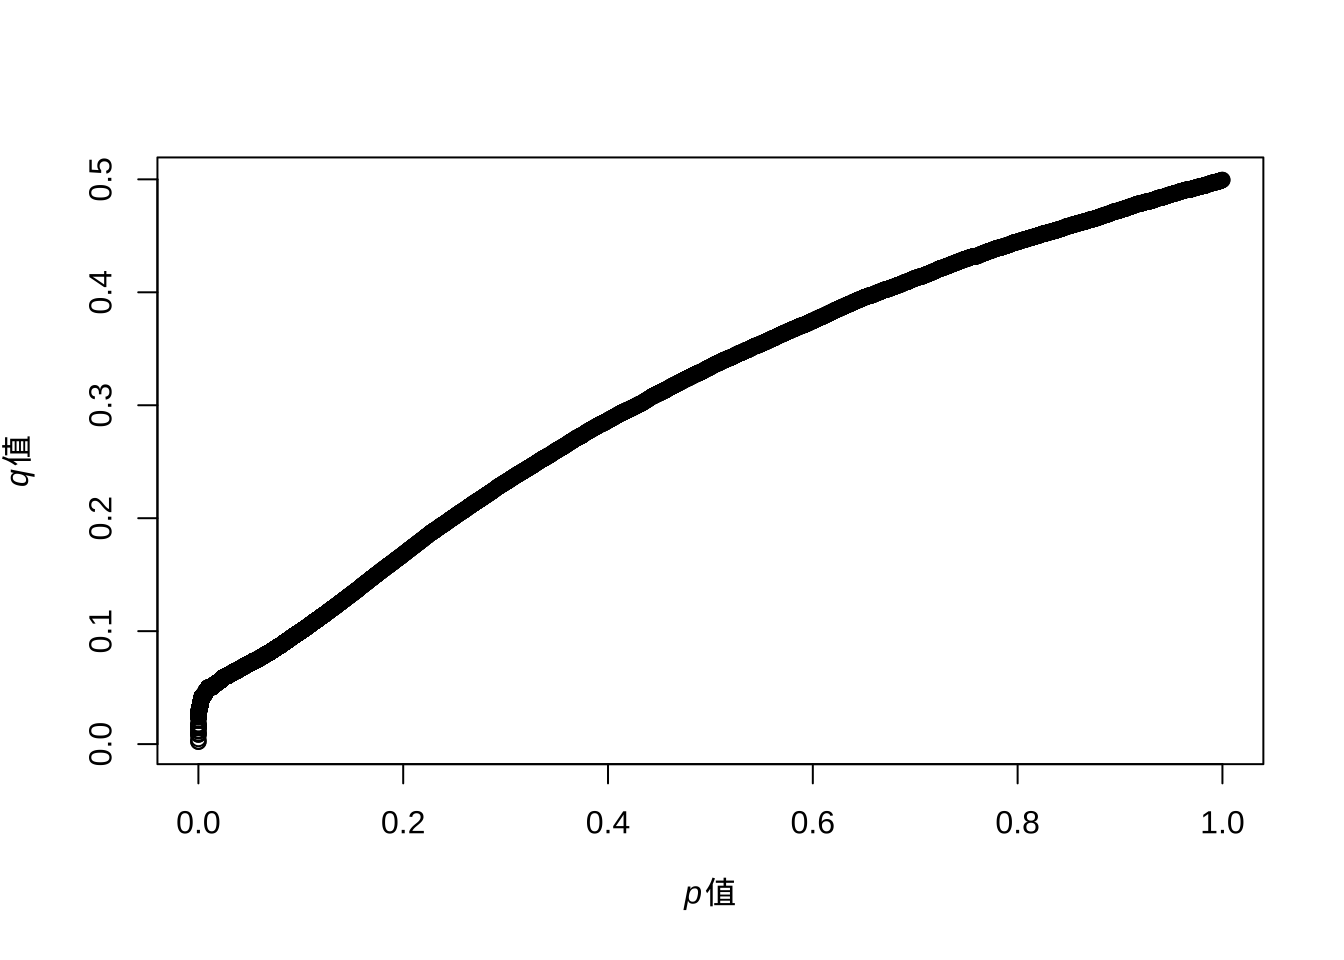
\includegraphics{sciguide_files/figure-latex/unnamed-chunk-29-1} \caption[p值与q值的变化]{p值与q值的变化}\label{fig:unnamed-chunk-29}
\end{figure}

如上图所示,q值增大后会最终逼近到0.5,而我们的模拟中零假设的比例就设定就是50\%。我们重新模拟一个零假设比例5\%的实验:

\begin{Shaded}
\begin{Highlighting}[]
\FunctionTok{set.seed}\NormalTok{(}\DecValTok{42}\NormalTok{)}
\NormalTok{pvalue }\OtherTok{\textless{}{-}} \ConstantTok{NULL}
\ControlFlowTok{for}\NormalTok{ (i }\ControlFlowTok{in} \DecValTok{1}\SpecialCharTok{:}\DecValTok{500}\NormalTok{) \{}
\NormalTok{  a }\OtherTok{\textless{}{-}} \FunctionTok{rnorm}\NormalTok{(}\DecValTok{10}\NormalTok{, }\DecValTok{1}\NormalTok{)}
\NormalTok{  b }\OtherTok{\textless{}{-}}\NormalTok{ a }\SpecialCharTok{+} \DecValTok{1}
\NormalTok{  c }\OtherTok{\textless{}{-}} \FunctionTok{t.test}\NormalTok{(a, b)}
\NormalTok{  pvalue[i] }\OtherTok{\textless{}{-}}\NormalTok{ c}\SpecialCharTok{$}\NormalTok{p.value}
\NormalTok{\}}
\ControlFlowTok{for}\NormalTok{ (i }\ControlFlowTok{in} \DecValTok{1}\SpecialCharTok{:}\DecValTok{9500}\NormalTok{) \{}
\NormalTok{  a }\OtherTok{\textless{}{-}} \FunctionTok{rnorm}\NormalTok{(}\DecValTok{10}\NormalTok{, }\DecValTok{1}\NormalTok{)}
\NormalTok{  b }\OtherTok{\textless{}{-}} \FunctionTok{rnorm}\NormalTok{(}\DecValTok{10}\NormalTok{, }\DecValTok{1}\NormalTok{)}
\NormalTok{  c }\OtherTok{\textless{}{-}} \FunctionTok{t.test}\NormalTok{(a, b)}
\NormalTok{  pvalue[i }\SpecialCharTok{+} \DecValTok{500}\NormalTok{] }\OtherTok{\textless{}{-}}\NormalTok{ c}\SpecialCharTok{$}\NormalTok{p.value}
\NormalTok{\}}
\NormalTok{pbh }\OtherTok{\textless{}{-}} \FunctionTok{p.adjust}\NormalTok{(pvalue, }\AttributeTok{method =} \StringTok{\textquotesingle{}BH\textquotesingle{}}\NormalTok{)}
\NormalTok{q }\OtherTok{\textless{}{-}} \FunctionTok{qvalue}\NormalTok{(pvalue)}
\FunctionTok{plot}\NormalTok{(pbh }\SpecialCharTok{\textasciitilde{}}\NormalTok{ pvalue,}
     \AttributeTok{ylab =} \StringTok{\textquotesingle{}错误发现率(FDR)\textquotesingle{}}\NormalTok{,}
     \AttributeTok{xlab =} \FunctionTok{substitute}\NormalTok{(}\FunctionTok{paste}\NormalTok{(}\FunctionTok{italic}\NormalTok{(}\StringTok{\textquotesingle{}p\textquotesingle{}}\NormalTok{), }\StringTok{"值"}\NormalTok{)),}
     \AttributeTok{pch =} \DecValTok{15}\NormalTok{)}
\CommentTok{\# Q值}
\FunctionTok{points}\NormalTok{(q}\SpecialCharTok{$}\NormalTok{qvalues }\SpecialCharTok{\textasciitilde{}}\NormalTok{ pvalue, }\AttributeTok{pch =} \DecValTok{16}\NormalTok{, }\AttributeTok{col =} \StringTok{\textquotesingle{}grey\textquotesingle{}}\NormalTok{)}
\FunctionTok{legend}\NormalTok{(}
  \StringTok{\textquotesingle{}bottomright\textquotesingle{}}\NormalTok{,}
  \FunctionTok{c}\NormalTok{(}\FunctionTok{expression}\NormalTok{(}\FunctionTok{paste}\NormalTok{(}\FunctionTok{italic}\NormalTok{(}
    \StringTok{"q"}
\NormalTok{  ), }\StringTok{" 值"}\NormalTok{)), }\StringTok{\textquotesingle{}BH 法\textquotesingle{}}\NormalTok{),}
  \AttributeTok{pch =} \FunctionTok{c}\NormalTok{(}\DecValTok{16}\NormalTok{,}\DecValTok{15}\NormalTok{),}
  \AttributeTok{col =} \FunctionTok{c}\NormalTok{(}\StringTok{\textquotesingle{}grey\textquotesingle{}}\NormalTok{,}\StringTok{\textquotesingle{}black\textquotesingle{}}\NormalTok{)}
\NormalTok{)}
\end{Highlighting}
\end{Shaded}

\begin{figure}
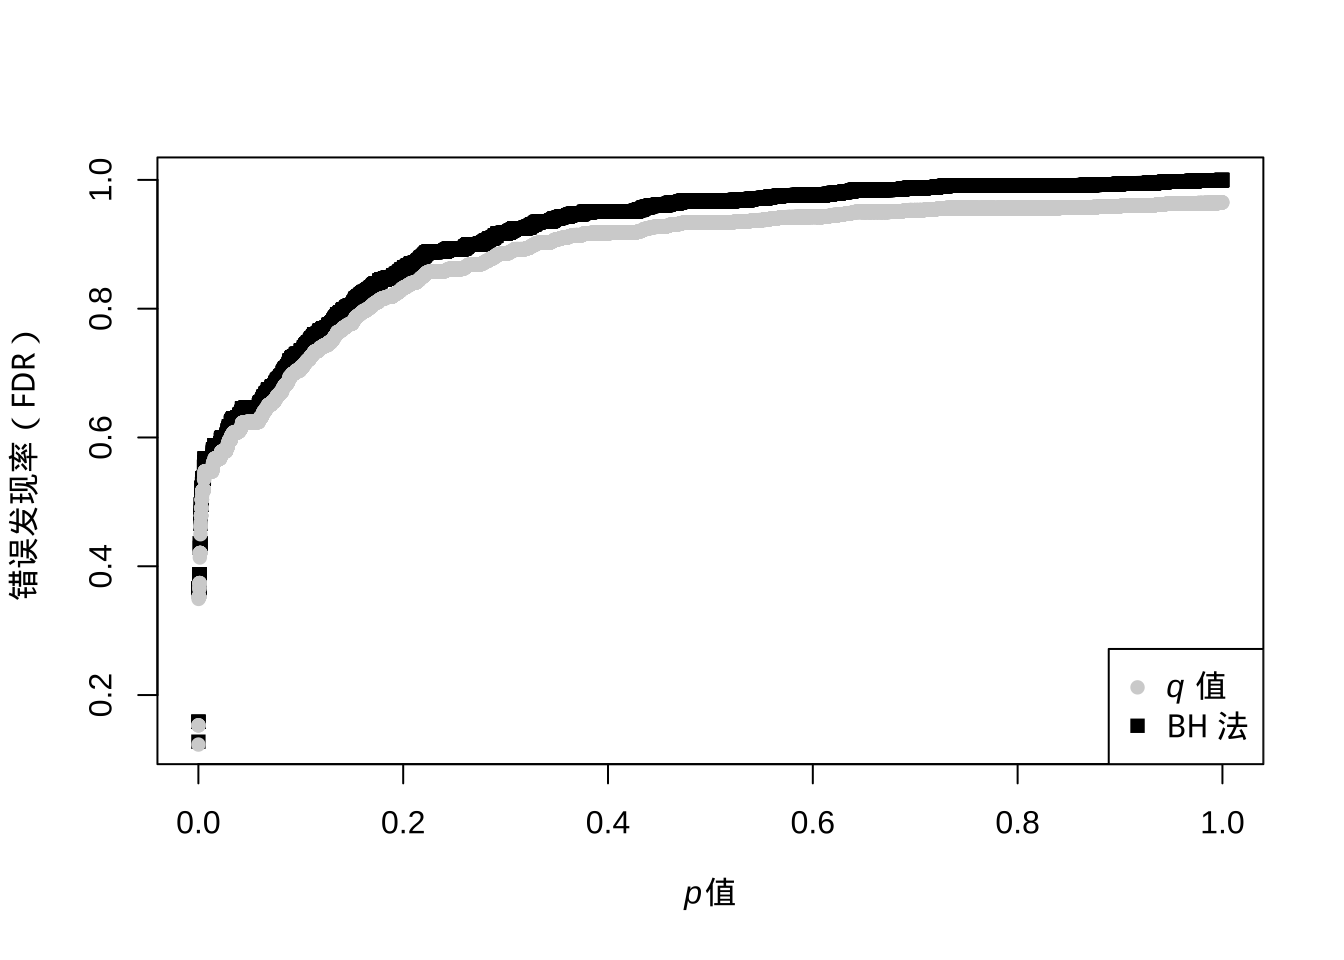
\includegraphics{sciguide_files/figure-latex/unnamed-chunk-30-1} \caption[q值与BH法下p值与错误发现率的变化]{q值与BH法下p值与错误发现率的变化}\label{fig:unnamed-chunk-30}
\end{figure}

此时我们可以看到两者结果较为接近,q值理论上更完备,功效也更强,但算法上对\(\hat\pi_0\)的估计并不稳定,特别是比例靠近1的时候,所以BH方法可能还是更容易让人接受的保守错误发现率控制方法。

多重检验问题是高通量数据里逃不掉的问题,要想找出真正的差异数据就要面对假阳性跟假阴性问题,这是一个不可兼得的过程,看重假阳性就用整体错误率,看重假阴性或功效就用错误发现率控制。并不是说哪种方法会好一些,更本质的问题在于你对实际问题的了解程度及统计方法的适用范围。实验设计本身就会影响数据的统计行为,而这个恰恰是最容易被忽视的。

\hypertarget{ux7ebfux6027ux6a21ux578b}{%
\section{线性模型}\label{ux7ebfux6027ux6a21ux578b}}

几乎所有的统计推断都可以放到统计模型里讨论,如果需要可进一步进行预测。科研中最常用的统计模型是\href{https://cosx.org/2019/09/common-tests-as-linear-models/}{线性模型},很多常见的统计推断方法都可以用线性模型的框架来解释。例如双样本t检验可算作方差分析的特例,方差分析可以看作带有伪变量的回归,协方差分析可以看作回归中的交互作用\ldots{}

线性模型的基本形式就是因变量是由自变量作用加和而成,在这个语境下,其实把自变量改为变量,放宽独立性限制,也能将一些非线性部分,例如高幂次的自变量及变量间的乘积或交互作用考虑进去。在实际问题的抽象上,只要可以把目标数值的变动用其他数值的拆解或组合表示出来,那么可以粗略认为标准化后其他数值的回归系数可用来比较不同数值间的贡献,而对于该系数的显著性检验则可以说明该系数的影响是否显著。

打个比方,流行病学里常说的某种疾病发病率或风险比在考虑了人群性别、年龄、BMI、吸烟史等的影响后发现某污染物起了显著影响,这就是说在一个目标变量为病发病率或风险比的线性模型中,性别、年龄、BMI、吸烟史作为协变量而污染物作为自变量,模型拟合结束后发现污染物的系数经假设检验为显著差异于零,也就是没影响。这里,协变量与自变量在回归上是平等的,可以把协变量理解为控制变量,如果你考察吸烟的影响,那么吸烟与否就是自变量,包含污染物在内其他项就成了协变量。不过所有考察变量选择的原则在于其理论上或经验上被认为与目标变量有关系且无法通过随机采样、配对等手段消除影响,这种情况对于观测数据比较常见。

在线性模型中,如果我们将两个共相关的变量放到同一个线性回归模型之中,那么这两个变量的系数估计的标准误都会扩大。下面我们展示下这个干扰过程:

\begin{Shaded}
\begin{Highlighting}[]
\FunctionTok{set.seed}\NormalTok{(}\DecValTok{42}\NormalTok{)}
\NormalTok{a }\OtherTok{\textless{}{-}} \FunctionTok{runif}\NormalTok{(}\DecValTok{100}\NormalTok{,}\AttributeTok{min=}\DecValTok{0}\NormalTok{,}\AttributeTok{max=}\DecValTok{10}\NormalTok{)}\SpecialCharTok{+}\FunctionTok{rnorm}\NormalTok{(}\DecValTok{100}\NormalTok{)}
\NormalTok{b }\OtherTok{\textless{}{-}}\NormalTok{ a}\SpecialCharTok{*}\FloatTok{1.2}\SpecialCharTok{+}\FunctionTok{rnorm}\NormalTok{(}\DecValTok{100}\NormalTok{)}
\NormalTok{c }\OtherTok{\textless{}{-}}\NormalTok{ b}\SpecialCharTok{*}\FloatTok{1.2}\SpecialCharTok{+}\FunctionTok{rnorm}\NormalTok{(}\DecValTok{100}\NormalTok{)}
\NormalTok{y }\OtherTok{\textless{}{-}}\NormalTok{ a}\SpecialCharTok{+}\NormalTok{b}\SpecialCharTok{+}\NormalTok{c}\SpecialCharTok{+}\FunctionTok{rnorm}\NormalTok{(}\DecValTok{100}\NormalTok{)}
\end{Highlighting}
\end{Shaded}

上面我们由两个变量生成了一个新变量,然而这两个变量是相关的,此时我们进行回归分析:

\begin{Shaded}
\begin{Highlighting}[]
\FunctionTok{summary}\NormalTok{(}\FunctionTok{lm}\NormalTok{(y}\SpecialCharTok{\textasciitilde{}}\NormalTok{a))}
\end{Highlighting}
\end{Shaded}

\begin{verbatim}
## 
## Call:
## lm.default(formula = y ~ a)
## 
## Residuals:
##     Min      1Q  Median      3Q     Max 
## -4.1929 -1.9935 -0.2595  1.9301  5.3011 
## 
## Coefficients:
##             Estimate Std. Error t value Pr(>|t|)    
## (Intercept) -0.14295    0.44101  -0.324    0.747    
## a            3.65619    0.07162  51.048   <2e-16 ***
## ---
## Signif. codes:  0 '***' 0.001 '**' 0.01 '*' 0.05 '.' 0.1 ' ' 1
## 
## Residual standard error: 2.339 on 98 degrees of freedom
## Multiple R-squared:  0.9638, Adjusted R-squared:  0.9634 
## F-statistic:  2606 on 1 and 98 DF,  p-value: < 2.2e-16
\end{verbatim}

\begin{Shaded}
\begin{Highlighting}[]
\FunctionTok{summary}\NormalTok{(}\FunctionTok{lm}\NormalTok{(y}\SpecialCharTok{\textasciitilde{}}\NormalTok{a}\SpecialCharTok{+}\NormalTok{b}\SpecialCharTok{+}\NormalTok{c))}
\end{Highlighting}
\end{Shaded}

\begin{verbatim}
## 
## Call:
## lm.default(formula = y ~ a + b + c)
## 
## Residuals:
##      Min       1Q   Median       3Q      Max 
## -2.10681 -0.69646 -0.06907  0.66959  2.31841 
## 
## Coefficients:
##             Estimate Std. Error t value Pr(>|t|)    
## (Intercept) -0.03088    0.18341  -0.168    0.867    
## a            1.20491    0.12910   9.333 4.03e-15 ***
## b            0.69905    0.16038   4.359 3.28e-05 ***
## c            1.11364    0.10523  10.583  < 2e-16 ***
## ---
## Signif. codes:  0 '***' 0.001 '**' 0.01 '*' 0.05 '.' 0.1 ' ' 1
## 
## Residual standard error: 0.9716 on 96 degrees of freedom
## Multiple R-squared:  0.9939, Adjusted R-squared:  0.9937 
## F-statistic:  5194 on 3 and 96 DF,  p-value: < 2.2e-16
\end{verbatim}

这里我们可以看到,如果只把第一个变量放入模型,那么斜率理论上应该是3.6。但此时我们把跟这个变量相关的另外两个变量放进去后回归模型对三个相关变量的系数估计都不再准确(应该都是1),标准误也扩大了。这个现象对理解线性模型非常重要,如果我们任意在线性模型里加入变量,变量间的随机相关会导致整个模型的回归系数估计性能都下降。因此线性模型不能随意加减自变量,最好事先考察自变量间的关系。

当线性模型的自变量只有一项时,其实考察的就是自变量与响应变量间的相关性。当自变量为多项时,也就是多元线性回归,考察的是你自己定义的``自变量''与``协变量''还有响应变量的关系。如果自变量间不能互相独立,那么最好将独立的部分提取出来作为新的变量,这种发现潜在变量的过程归属于因子分析,可以用来降维。自变量本身存在随机性,特别是个体差异,这种随机性可能影响线性模型自变量的系数或斜率,也可能影响线性模型的截距,甚至可能同时影响,此时考虑了自变量的随机性的模型就是线性混合模型。线性混合模型其实已经是层级模型了,自变量的随机性来源于共同的分布。如果自变量间存在层级,例如有些变量会直接影响其他变量,那么此时线性模型就成了决策/回归树模型的特例了。如果层级关系错综复杂,那不依赖结构方程模型是没办法搞清楚各参数影响的。然而模型越复杂,对数据的假设就越多,对样本量的要求也就越高。同时,自变量或因变量有些时候也要事先进行连续性转换,这就给出了logistics回归、生存分析等特殊的回归模型。科研模型如果是依赖控制实验的,那么会在设计阶段随机化绝大部分变量,数据处理方面到线性混合模型就已经很少见了。

但对于观测数据,线性混合模型只是起点,对于侧重观察数据的社会科学研究,样本量与效应大小是结论可靠性的关键,精细的模型无法消除太多的个体差异。这种复杂关系走到极端就是网络分析了,网络分析适合用来研究多样本或特性间的关系,这类关系通常用互相连接的节点来表示,在可视化中节点一般指代一个样本或特性,连线则代表了样本间或特性间的关系。说白了网络分析是另一层意义上的因子分析,起一个降维作用,只是降维方式不是简单的线性组合而是引入了图论的一些统计量。

高维数据是线性模型的一大挑战,当维度升高后,变量间要么可能因为变异来源相似而共相关,要么干脆就是随机共相关。在某些场景下,高维数据可能都没有目标变量,需要先通过探索性数据分析找出样本或变量间的组织结构。这种场景下应通过变量选择过程来保留独立且与目标变量有潜在关系的变量。也就是说,变量选择的出发点是对数据的理解,优先考虑相关变量而非简单套用统计分析流程。当然,统计方法上也有变量选择的套路,评判标准可能是信息熵或模型稳健度的一些统计量,可以借助这些过程来简化模型或者说降维。对于线性模型而言,就是均方误、Mallow's \(C_p\)、AIC、BIC还有调节R方等,可借助回归模型软件来完成。

回归或模型拟合都存在过拟合的风险,所谓过拟合,就是模型对于用来构建模型的数据表现良好,但在新数据的预测性上却不足的情况。与过拟合对应的是欠拟合,此时拟合出的模型连在构建模型的数据验证上表现都不好。这里的表现可以用模型评价的一些指标,其实跟上面进行变量选择的指标是一样的,好的模型应该能捕捉到数据背后真实的关系,也因此在训练数据与新数据上表现一致。

在统计学习领域里,工程实践上最简单的验证过拟合与欠拟合的方法就是对数据进行切分,分为用来构建模型的训练集与验证模型预测性能的检测集,更细的分法则将检测集分为可在模型调参过程中使用多次的检测集与最后最终评价模型的一次性验证集,三者比例大概6:3:1,也可根据实际情况来定。也就是说,模型的构建不是一次性完成的,而是一个反复调整模型参数的过程来保证最终的模型具备良好的预测性与稳健度。

在技术层面上,调参过程有两种基本应对方法,第一种是重采样技术,第二种是正则化,两种方法可以组合使用。重采样技术指的是通过对训练集反复采样多次建模来调参的过程。常见的重采样技术有留一法,交叉检验与bootstrap。留一法在每次建模留一个数据点作为验证集,重复n次,得到一个CV值作为对错误率的估计。交叉检验将训练集分为多份,每次建模用一份检验,用其他份建模。bootstrap更可看作一种思想,在训练集里有放回的重采样等长的数据形成新的数据集并计算相关参数,重复多次得到对参数的估计,计算标准误。在这些重采样技术中,因为进行的多次建模,也有多次评价,最佳的模型就是多次评价中在验证集上表现最好的那一组。

正则化则是在模型构建过程中在模型上对参数的效应进行人为减弱,用来降低过拟合风险。具体到线性模型上,就是在模型训练的目标上由单纯最小化均方误改为最小化均方误加上一个对包含模型参数线性组合的惩罚项,这样拟合后的模型参数对自变量的影响就会减弱,更容易影响不显著,如果自变量过拟合的话就会被这个正则化过程削弱。当惩罚项为模型参数的二次组合时,这种回归就是岭回归;当惩罚项为模型参数的一次绝对值组合时,这种回归就是lasso;当惩罚项为一次与二次的组合时,这种回归就是弹性网络回归。实践上正则化过程对于降低过拟合经常有神奇效果,同时正则化也可作为变量选择的手段,虽然岭回归无法将系数惩罚为0,但lasso可以,这样在参数收缩过程中也就同时实现了变量选择。

为了说明实际问题,有时候单一形式的模型是不能完全捕捉数据中的变动细节的,我们可以在工程角度通过模型组合来达到单一模型无法达到的预测性能。模型组合的基本思想就是对同一组数据生成不同模型的预测结果,然后对这些结果进行二次建模,考虑在不同情况下对不同模型预测结果给予不同的权重。这种技术手段可以突破原理限制,而最出名的例子就是人工神经网络里不同神经元采用不同核函数的做法了。

对于科研数据的线性回归,还有两个常见问题,一个是截断问题,另一个是缺失值处理。截断问题一般是采样精度或技术手段决定的,在数值的高位或低位无法采集高质量数据,此时可以借助截断回归等统计学方法来弥补。另一种思路则是在断点前后构建不同的模型,这样分别应对不同质量的数据。对于数据缺失值的问题,统计学上也提供了很多用来删除或填充缺失值的方法,填充数据不应影响统计推断,越是接近的样本,就越是可以用来填充缺失值,当然这个思路反着用就是个性化推荐系统模型的构建了。

除了线性模型,非线性模型在某些研究中也经常用,特别是对一些机理的验证上,经常要拟合S型曲线,此时模型的形式往往是固定的,用来给出一些过程中重要的参数。但如果你打算提出新的模型,就要认真考虑这些模型参数的物理意义及新模型如何在这个过程中逻辑上说通。非线性模型包括凸函数与凹函数,最常见凸函数是指数函数,掌握72法制,也就是72除以速率大概就是翻倍用的时间。最常见凹函数是收益递减函数,平均价值大于价值的平均,具有风险规避特性。例如劳动力和资本凹函数,新的投资得到的收益会越来越低。

\hypertarget{ux6a21ux578bux7ec4ux5408}{%
\section{模型组合}\label{ux6a21ux578bux7ec4ux5408}}

线性模型是科研中最常见的数据分析模型,但伴随机器学习算法的兴起,各类预测模型都可以嵌入到科研数据分析之中解决具体的科学问题。此时我们除了可以尝试不同类型的数据分析模型之外,我们也可以对这些模型的预测结果进行组合来进一步提高预测性能。此时我们可能要放弃掉线性模型的可解释性而更多关注组合模型的预测准确性与鲁棒性。

在讨论模型组合策略前,首先要熟悉不同模型对数据结构的假设。线性模型如果跟线性模型组合在一起,相当于在同一个模型里加了两个共相关自变量,很可能导致组合后的模型还不如之前的模型效果好。常见的模型组合策略基本假设就是不同模型提取了数据中不同角度的信息,线性模型捕捉的是自变量与响应间加性关系、决策树模型捕捉的是自变量与响应间的层级结构、多项式模型捕捉的是自变量与响应间的非线性高阶关系、神经网络捕捉的是不同核函数假设下自变量与响应间的复杂关系等,甚至深度学习可以看做用一个层次数不断叠加的巨大神经网络来捕捉数据中可能存在的模式。有时候神经网络跟其他模型组合时表现反而下降,原因就在于神经网络已经捕捉到了其他模型的模式,加进去其实是降低了预测模型的稳健度。因此,如果要进行模型组合,一定要对待组合的模型有原理上的理解,否则很可能适得其反。

模型组合策略其实已经体现在很多机器学习算法之中了,特别是随机森林算法里就体现了小模型组合这类思想。实践中进行模型组合是可以体现在不同步骤里的,例如我可以把训练集切成若干份,每一份用一种模型训练,预测的时候是针对不同模型预测结果进行加权综合。当然也可以在训练集上训练所有的模型,然后对结果进行综合,甚至还可以事先利用相关性或聚类把变量分组,然后不同组变量用不同模型预测,这就类似广义线性模型的思路了。具体选择哪种组合策略也可以去寻优,理论上组合策略是无穷的且很难说哪种策略是通用且最好的,最好的组合策略一定是最能挖掘数据信息的那一种。

模型组合策略也可以用来进行解释性研究。最简单的例子就是在线性模型里加上一个二次项发现拟合效果变好了,那么可能暗示数据内在结构就是一个多项式模型。另一种解释方法则是对不同模型的预测结果的残差分布进行研究,看看具体哪一种模型加入后残差分布更接近噪声的正态分布,这样可以去推测数据中起主要作用的模型是哪一种,进而通过模型假设反推数据中存在的主要模式或结构。这种探索性分析一定要做好做足而不是简单去套数据分析模版,套模版是很难发现新模式的。

\hypertarget{ux8ba1ux7b97ux65b9ux6cd5}{%
\section{计算方法}\label{ux8ba1ux7b97ux65b9ux6cd5}}

科研数据处理通常以直观为首选,但样本量或维度上来之后计算效率就必须考虑,否则很多计算,特别是针对仿真数据算统计量的问题会非常慢,影响工作效率。此外,还有些之前被认为实际算不了的问题现在其实也能算了,很多计算工作只要你转化得当都可以在高性能计算平台的应用层上实现。这里简单介绍一些现代计算方法与趋势,了解概念后可以寻求专业人士来合作,拓展研究广度。

\hypertarget{ux5e76ux884cux8ba1ux7b97}{%
\subsection{并行计算}\label{ux5e76ux884cux8ba1ux7b97}}

并行计算是当前科学计算提速的最简单方案。不是所有的任务都可以并行计算,并行计算的任务要可以进行切分,之后分发到各个独立计算单元计算后汇总,实现快速计算,顺序执行的计算任务可以分拆给不同计算机,但这不叫并行计算了。计算任务的并行是逻辑层上的,现实中可能是单核多线程并行,多核多线程并行,多终端多核多线程并行,计算结果汇总后输出结果。作为用户我们需要告诉计算机任务并行方式,很多并行计算的软件会自动配置管理,我们只要逻辑上定义好并行计算任务就可以了,不过有时候需要手动配置,此时起码知道并行化是在哪个层次上。

并行计算并不需要多机运行,有时候如果你能有效利用单机多核或多进程例如OpenMP就可以实现单机效率提升。如果你的计算任务不是很复杂就是量比较大,可以尝试GPU加速。图像天生就可以并行化处理,例如切成16*16矩阵,然后送到256核GPU一对一并行处理每个矩阵的变化,这比把图像向量化送CPU速度就有了质的提升。不过GPU的指令集比CPU小很多,所以太复杂的计算并不适合GPU加速,但如果可以GPU加速,效果非常魔幻,可尝试CUDA这个计算框架。多机运行的并行运算通常会在应用层定义好独立计算单元的分布,然后由计算框架例如snow去做任务分发。多机器临时集群可以跨主机分布或进行云计算,需要指定名称,可通过 传统 socket 或符合MPI标准的方式来组建。

在具体运行函数上,要依赖软件或编程语言的支持,有些函数已经进行了并行化优化可直接调用,有些需要声明用法才能调用。不论你用什么软件,想并行化是需要针对性做配置的,并不是你提供一台多核多线程的电脑它就自动会并行化计算,虽然大趋势确实是打算自动化,但科研计算问题通常要自己动手设计这个过程。

\hypertarget{ux5bb9ux5668ux6280ux672f}{%
\subsection{容器技术}\label{ux5bb9ux5668ux6280ux672f}}

另一个与计算相关的问题是虚拟化技术,更具体的说是容器技术。容器技术本质上就是打造一个包含用户界面、软件及系统的高可移植度系统镜像,从而实现工作环境的快速部署。这对于科学计算的意义在于本身极高的用户友好度与研究中计算部分的可重现性,科研人员或实验室可以快速分发最新研究成果,省略掉中间海量技术细节。同时容器技术不但可以本机部署,也可以远程部署,这使得临时组建集群进行有弹性的计算变得可能,也降低了成本。容器技术例如 Docker 是值得现代科研人员掌握的数据分析技能。

容器化或虚拟化更底层其实是功能模块化。目前很多计算模块还有系统间的接口都实现了标准化,科研人员可按照需求一层层搭建自己的计算环境。目前也出现了以解决方案为核心的咨询或服务商来辅助实验室设计这样的计算环境或容器或模块,不过虽然技术调配可以找专业人士,计算框架的逻辑科研人员必须掌握原理。

\hypertarget{ux4e91}{%
\subsection{云}\label{ux4e91}}

云技术包括云计算与云存储,这背后的趋势是科研产业跟其他行业的快速融合与迭代。相比传统购买工作站、服务器或自己搭建计算集群,现代科研计算可以用成本更低的方法,也就是租赁计算资源与存储资源,只为自己使用的机时与存储付费,不用亲自维护计算资源的更新换代。

云计算可以直接去租大型互联网公司提供的资源或机构内搭建的高性能计算集群。云存储则可以通过云端实时备份来保证数据安全。对于数据安全性要求高的研究,可以自己组装包含NAS的个人云在局域网内备份数据。科研云计算大趋势是租资源,用完释放,这对于经费有限的中小课题组是重要生存技能。

\hypertarget{ux4e3bux6210ux5206ux5206ux6790}{%
\section{主成分分析}\label{ux4e3bux6210ux5206ux5206ux6790}}

主成分分析应该是科研领域里最通用的一种数据分析手段。很多人认为这种方法主要是用来进行探索分析的可视化手段与数据降维,但这个方法其实四通八达,可以把很多数据分析的概念连接起来。

首先还是回到一个最简单的场景,我有一堆数,想找出一个来做代表。从距离测量角度,就是找一个点让它离所有点最近,这就成了个优化问题,此时不同测量方法结论是不一样的。例如你考虑距离的绝对值最小,那你就会得到中位数;如果是差异的平方,求导后就是均值。回想下对一堆数找一个数,其实就是一种降维,从1维降低到0维。这里我们只考虑最小化差异的平方,那么求均值就是主成分分析把从1维降低到0维的应用场景。

现在复杂一点,我们设想一个二维平面,如果我们对其降维,那么降一维就是线,降两维就是点。而且我们可以确定降两维的那个点肯定就在降一维的线上,不然你这个降维就丧失了代表性。至于如何保障代表性,一般来说要交给数学家。那么这条线会通过所有点的均值,此时你应该想起来二维线性回归也通过这个点,那条线可以通过最小二乘得到,会不会就是我们要找的那条线?这个答案是否定的,最小二乘里最小化的是因变量到回归线的值,但是这里主成分分析最小化的是所有点到一条线的垂直距离,模型上细微的差别导致结果也会有区别,事实上求解过程也不对等。

虽然最小二乘回归线是高斯-马尔可夫定理下线性回归的最佳无偏估计,但主成分分析里二维降一维里那条线的求解思想并非回归到均值,常见有两种解释。第一种是寻找低维度空间,使投影点上到高维度点距离最近;另一种则是从统计角度寻找让点之间方差最大的方向映射,然后寻找跟这个方向正交的方向中方差最大的方向继续映射。从求解上,这两种解释都可转化成最优化问题,都是先归一化,然后求协方差矩阵,通过求导求特征向量跟特征值,那个方差最大的方向或距离最短子空间维度就是协方差矩阵里特征值最大的特征向量,剩下的方向或维度跟前面那个正交,再次找方差最大或距离最小即可。当然协方差矩阵不是一定要求的,如果你选用奇异值分解的套路就完全不用求。在这个求解策略下,解析解就是正交的,如果不是,那就不是主成分分析了。

除此之外,理论上你也可以用隐藏变量模型迭代求解,不过有解析解不要用数值分析去逼近,而且有些矩阵运算可以进行分布式计算,这个在数据量大时是要特别考虑的。主成分分析求解上可以用矩阵是很大的优势,虽然理论上其概率解释并不完美。不同求解思想的多元分析方法其实背后都是有思想跟应用场景的,虽然理论上很多都是通用方法,但如果不适合你的数据就不要用。当前由于技术进步,之前很多很耗性能的方法目前都可以计算得到,如果搞科研我们要找那个最完美的,但工业应用可能更看重性价比。

如果我们进一步考察三维空间,那么我们的降维就首先是一个平面,然后是平面上的线,然后是线上的点。此时如果你对所有数据点乘2,那么很自然点、线、面的坐标位置都要变化,这样你就可以理解一个事实,那就是主成分分析对尺度是敏感的,所以一般来说都要对不同尺度/维度的测量进行归一化,否则你的映射会被大尺度的维度带跑偏。到现在为止,我们可以大概对主成分分析有个直观感受:将高维度空间的点映射到低纬度空间的点且要保证这些点之间的差异关系最大程度地保留,至于怎么保留,不同求解思想实际求解结果一致,都可以用矩阵运算,内含了进行转换或映射时要沿着正交的维度走(使用了正定阵),所以求解完矩阵就可以得到符合要求的低维度空间,而且低维空间是正交的。

主成分分析经常用来可视化,这里我们回到二维平面降维的场景仔细看看我们究竟可视化了什么。首先我们有一个二维点A,这个点投影到一维线上得到点B,这个点跟所有点的均值C连线就是到0维的投影。目前我们已知AC这个线,同时A到一维线的距离又要最小也就是垂直,这样A、B及C构成一个直角三角形。此时根据勾股定理BC这个距离最大,也就是一维到0维时所有投影点的距离之和最长,在这个方向中各点间方差最大程度保留,也就是找到了方差最大的方向。事实上,因为前面提到的直角三角形,每降低一次维度,点之间的距离比高维度都不可避免的减少,如果此时点聚到一起不一定相似度很高,但如果主成分占总方差比重比较大,那么这些点就很有可能十分相似。

\begin{figure}
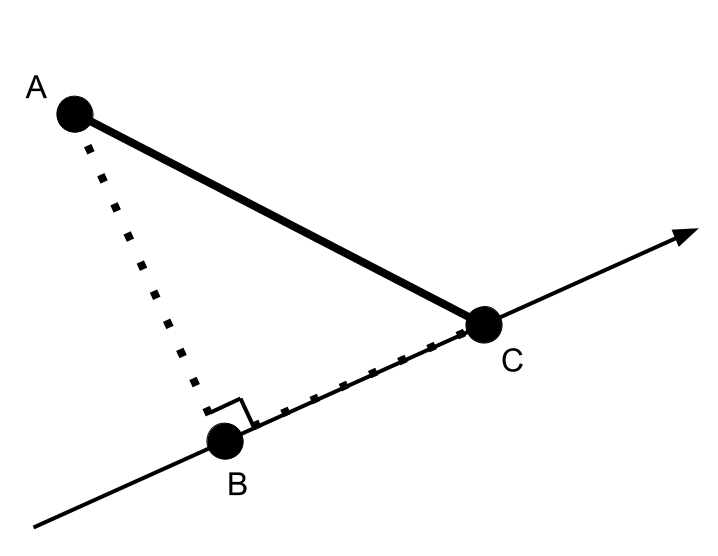
\includegraphics{data/PCA} \caption[二维对一维的投影示例(A为二维数据点,C为所有点在一维上的投影均值,AC固定下AB垂直于一维时AB最短,勾股定理下BC最长,也就是方差最大的方向)]{二维对一维的投影示例(A为二维数据点,C为所有点在一维上的投影均值,AC固定下AB垂直于一维时AB最短,勾股定理下BC最长,也就是方差最大的方向)}\label{fig:unnamed-chunk-33}
\end{figure}

说到距离,其实主成分分析也是多维标度分析(MDS)的一种。在经典多维标度分析中,测定点很困难,但可以测到点之间欧式距离并构建距离矩阵,因为其映射子空间里点之间方差最大时可以证明点之间的距离也是最大的,这个特性保证了当我们只有距离矩阵时进行主成分分析得到的低维映射也可以保证两个空间间距离最短,这样主成分分析事实上符合经典多维标度分析。也就是说,在你能够测到欧式距离而不是点时,是有可能重构出原始标度的。

主成分分析在求解上基本都走了矩阵运算的捷径,结果也是等价的。但这个过程不算是一个概率模型,因为可能产生不确定度的白噪声根本没出现在求解模型中。此时,我们应该意识到,这个子空间可能是某个概率模型的解,但如同我们只求了均值没求方差一样,似乎我们没有考虑模型的不确定度。这样我们需要从统计角度把主成分分析统一到基于统计学的数据分析中,这样也许会对将来构建相关假设检验模型有用,当然这也意味着我们可能不太方便再用矩阵运算来求解了。

首先,我们对数据点进行假设,例如来自一个正态分布,那么主成分分析的问题就转化为求一个子空间,使得映射后的距离最小。让我们把这个映射关系描述成下面这样:

\[
t = Wx + \mu + \epsilon
\]

这里t是我们观察到的数据点,W是映射关系,维度不变可以理解成坐标轴旋转,x是映射后的点,\(\mu\)代表x的均值,\(\epsilon\)代表高斯随机变量。这样我们看到的点符合均值\(\mu\),方差\(WW^t + \psi\)的正态分布,这里\(\psi\)代表了随机误差,如果我们不考虑这一项,那么主成分分析是完全可以用特征值跟特征向量求解的,此时我们默认那个误差项0方差。但是,实际场景中我们都很清楚每一个高维样本点都至少存在测量误差,这个误差的方差不是0,那么此时我们应该在模型中包含误差项,但一个很尴尬的问题是我们对这个误差一无所知。此时我们假定所有点的误差项来自于某一个方差统一的正态分布,然后有了这个限制条件就可以求解了。加入了这一部分后,主成分分析就可以进行假设检验了,例如某个点是否属于异常值。

说到求解EM算法是绕不过去的,这个算法普适性比较强,存在隐藏变量的模型求解都可以用。主成分分析可以看作一种存在隐藏变量的模型,我们在低维空间看到的点背后是高维空间点但看不到,反之也成立。这样我们先随意假设一个新空间出来,这样我们就可以进行E阶段计算,也就是把看到的点投影到这个新空间上,然后计算距离。之后我们就可以进行M阶段,也就是最小化距离,这样就做出了一个比起始新空间距离更小的空间。然后再进行E阶段,M阶段,直到距离无法缩小。说白了就是模型不存在时先人工创造一个,然后不断按你的目标迭代让模型跟数据契合。在EM算法里,我们就可以很轻松把前面的方差项也扔进去一同优化,最后也能求解。这样概率化的主成分分析就有解了。不过这个算法具体实现存在很高的技巧性,我们吃现成就可以了。同时你会发现,其实EM算法思想可以用在很多不同模型参数求解上,马尔可夫过程、贝叶斯网络、条件随机场等有隐含变量的都可以用。

其实在更多资料中引入概率化的主成分分析主要是为了引入因子分析,因子分析跟概率化主成分分析最大区别在于其不限制误差来自方差相同的正态分布。这当然增加了计算难度,但其实因子分析对于解释这种隐藏结构其实比主成分分析更靠谱。但是,因子分析求解上不如主成分分析容易理解,需要通过一些方法来决定因子数或干脆使用者自己决定。此外,因子分析是可以进行预测的,目标就是潜在因子。从概率角度讲主成分分析自然也可进行预测,不过你得想清楚应用场景。同时,因子分析得到的成分也是正交的,这点跟主成分分析一致。正交的优点在于映射之间不相关,但不一定独立,如果数据分布需要独立因素就需要独立成分分析。

独立成分分析在独立成分符合正态分布时其实就是主成分分析,但当你独立成分并不来自正态分布时,独立成分分析就更有优势将其反推出来。因为独立跟相关是不同的,独立在统计学里比不相关约束条件更强,不相关不一定独立但独立一定不相关,独立因素间的互信息为0或者说高阶统计量上都不相关。最经典的应用就是鸡尾酒会问题,在一个嘈杂的场景里很多人都在说话,你在固定位置放了几个麦克风,这样麦克风收集到的就是多种声音的混合,现在你需要把混音中每个人的声音提取出来。此时你要用主成分分析,你会得到所有人声音的共性,但独立成分分析就可以分辨出每个个体,或者说潜在变量,所以你也猜到了,EM算法也可以求解独立成分分析。需要注意的是独立成分分析不管降维,基本你设定分多少个就有多少个。但不论主成分分析、因子分析还是独立成分分析,本质上都是线性模型的结构,也就是所谓的主成分、因子、独立成分都是原始数据的线性组合。

有些论文用主成分分析搞聚类画圈圈来说明样品间存在内在共性。这个在环境分析中比较常见,因为环境分析通常同时测定上百种化合物,前面提到低维映射里最大程度保留了样品点的差异,此时映射到一起就有可能说明那些样品污染特征接近,便于探索来源或环境过程。实际上此时不一定需要局限在主成分分析,可以直接用聚类分析等统计模型。

很多人搞不清楚特征值、特征向量还有载荷等的细节,所以主成分分析就被用成了降维画图工具,但其实这个探索分析是针对背后隐藏变量的,具体到主成分分析就是共性。还是举个例子来说吧,我有100个样品,每个样品测了1000个指标,现在我就有了个\(100*1000\)的矩阵,通过主成分分析我得到了\(100*250\)的矩阵,这个矩阵包含了原数据95\%的方差。好了,现在我问你,这250个新指标是什么?对,特征向量,特征向量就是新投影方向,投影可以看作隐含共性。特征值又是什么,共性的权重,越大代表越重要,毕竟可以代表更多的方差。那么载荷又是什么,大概可以理解成原来1000个指标对250个新指标的贡献。那么进行分析时我们在样本和指标之间多了一个共性层,一方面减少了数据维度,另一方面算是提取了指标间不相关的共性(但不一定独立,切记)。对于多出来的共性层,我们同时知道样品在这些共性上的分布,也知道每个指标对共性的分布,常见的biplot就可以同时绘制样品点跟指标在两个最重要共性上的分布,一目了然。此时我们的专业知识就要上场了,我们可能会通过指标相互作用发现共性背后对应隐含因素的物理含义,也可以发现某种分离样品的共性背后暗示的样品潜在来源。总之,多了一个共性层后,我们可以研究的机理就更明显了,例如自然语言处理里可以用其寻找文本主题,基因组学里可以用来寻找基因模块等。但需要提醒的是,这个``共性''并不代表客观规律,只是一种线性变换后的结果,如果跟实际想研究的因素不对应还不如直接上回归分析。

主成分分析或者说实现主成分分析的奇异值分解的另一个应用就是可以用来压缩数据,上面的例子中100*1000的数据空间如果赶上稀疏矩阵十分浪费,此时就可以用奇异值分解压缩存储空间。从信号处理的角度去看,主成分分析跟傅立叶变换等变换过程本质上都是用一组新信号替代原来信号,由于一般认为信号方差高于噪声方差,通过变换时保留主成分或特定频谱,我们同时可以做到降噪。图形处理也可以用,而所有数据其实都可以用图形展示,那么作为图形降噪的主成分分析背后跟数据降噪是可以联系到一起的,特别环境痕量分析中的降噪。结合前面的结构重构、方差保留等性质,其实哪怕你就只会主成分分析,想明白了能做的事也很多。

\hypertarget{lib}{%
\chapter{文献}\label{lib}}

设计实验处理数据是科研的基本单元,但现代科研是需要互相借鉴参考的,文献就是最重要的参考依据。本章将首先讨论文献管理的步骤,然后通过实例讲解下现代文本挖掘技术在文献分析中的应用,之后会讨论下如何利用文献数据库进行全学科评价,了解自己研究在整体科研中的定位,最后会讨论下文献综述里最常用到的荟萃分析方法。

\hypertarget{ux6587ux732eux7ba1ux7406}{%
\section{文献管理}\label{ux6587ux732eux7ba1ux7406}}

文献管理方面主要包括文献收集、整理、分析与追踪,目的是获取当前研究趋势。用认知过程阶段可以分成三个:从无到有、从有到精与从精到用,从无到有是指刚进入一个新领域时的状态,绝大多数研究生跟转行的科研人员都要通过这个阶段构建自己的文献知识库;从有到精指维护与整理与追踪新文献;从精到用阶段指文献知识库体系直接参与科研过程形成产出的过程。

\hypertarget{ux4eceux65e0ux5230ux6709}{%
\subsection{从无到有}\label{ux4eceux65e0ux5230ux6709}}

刚开展研究工作的第一步就是背景知识的了解,除非你研究生转行,一般本科阶段的学习应该已经掌握了学科基础,这个是共通的背景知识。基于此你要从教科书上相对确定的知识走向文献资料中相对不那么确定的知识,此时最好的开端是一本英文教材,一方面锻炼英文,另一方面英文教材的更新比国内要快(你大概率可以从图书馆借到,而且多数图书馆都有根据你需求订书的服务,不要浪费)。如果你精力足够,甚至可以联系作者问下是否可以翻译,这样一举多得,不过我没操作过,只是建议。另一个思路是通过网络公开课 来系统学习,国内外很多高校放到网上的课程授课老师都属于接受新思想比较快的人,讲义也比较前沿,系统性比较高。还有一个不太通用的方法是阅读近些年的博士论文,其文献部分一般都是相关信息,不过能不能找到就不好说了。这个阶段一般要两三个月,不要心急,先把基础打好。前面掉的坑越多,后面跳坑就更有经验。

一般而言,一项学术成果要先发表,然后被综述评论,然后进入研究生课程讨论班,然后进入本科生课程讲义,最后才进入学科经典教材的更新。所以你可以倒着去走这个流程,越往后可能越不容易懂,但循序渐进总比一下读前沿论文被搞晕要好。有了相对前沿的教材或讲义作为知识框架,你的脑子里此时应该比较清楚导师让你做的东西或自己打算做的东西在学科中的定位,解决的是什么科学或工程问题,此时可以进行基于关键词检索的文献收集了。

一个良好的搜索返回的结果应该在10篇以内,首先要是综述,然后关键词检索方面建议学点逻辑运算符来过滤掉不相关信息,如果你上一阶段看的书是5年前更新的,那就只去关注最近5年的综述;如果你做的领域实在太新,那就把关键词信息的同义词跟近义词也加到搜索里;如果你能找到一篇写的特别好的综述或者有高人指点的论文,那是最高效的方法,可遇不可求。这10篇论文请按年为单位每1-2年选一篇综述去看,一月内读完,要求是精读,也就是论文里提到的研究都加到你的文献库里并阅读细节,同时可参考综述章节对文献库进行分组。一定要做笔记,而且要进行结构化的笔记或思维导图,这个阶段时间可能比较长也比较累,成果是当你去听系里的报告时,你大概能将报告定位到你的笔记框架里。考虑引用可以准备事实笔记与观点笔记,事实笔记是为了方便引用一个现象来论证你的问题而观点笔记则是方便引用结论来对比你的结论或讨论,后一种要特别小心,避免误会。到此文献库就从无到有了。

\hypertarget{ux4eceux6709ux5230ux7cbe}{%
\subsection{从有到精}\label{ux4eceux6709ux5230ux7cbe}}

有了文献库不代表就不用读了,你要建立一个体系来整理并追踪最新文献,可以通过加入邮件列表、新闻组或订阅期刊或数据库关键词的 RSS 来完成。信息收集有三个层次,最低就是关键词相关文献,这个主要依赖 RSS 或追踪重点课题组,关注这个可以保证对自己研究方向的掌握,不仅是期刊论文,预印本与会议论文也要关注到;中间层就是专业类顶级期刊,关注这部分信息可以对学科发展趋势有所了解;如果还有时间精力,可以关注综合类期刊,例如nature、pnas、science、NEJM、JAMA等,了解重大科学问题。

阅读文献时,要合理分配时间,科技文献已经\href{https://www.alternet.org/news-amp-politics/science-has-outgrown-human-mind-and-its-limited-capacities-process-information}{超越}了人脑处理信息的能力了。一般而言都要读题目, 20-50\%读摘要,5-10\%看图,1-3\%读全文。网上一般都可以找到摘要,如果需要全文,可以在 twitter 上用 \#icanhazpdf 标签找、可以用开源的\href{https://github.com/ropensci/fulltext}{fulltext}包找、可以用 \href{https://unpaywall.org/}{unpaywall} 的 API \href{https://cran.r-project.org/web/packages/roadoi/vignettes/intro.html}{找}、可以用\href{https://openaccessbutton.org/}{Open Access Button}的 API 来找、当然也可以找作者要或者找有权限的朋友帮忙。

文献管理可以借助专业文献管理软件,有收费的也有免费的,一般而言可通过咨询自己所在科研机构的图书馆来获取是否购买了相应的软件,一般图书馆也提供使用培训。早期文献管理软件之间差异还是明显的,但到今天基本同质化了。这里我要提示一下,一般文献库管理工具都提供针对单篇文献的笔记功能,不要用。请自建按研究主题的笔记,把新的有意思的新论文连同你以后可能引用的语句直接摘到相关主题的笔记里,而且要让你的笔记可以反链到数据库或通过 doi 可以直接找到原文(推荐后者)。没别的意思,我希望你的笔记稍加整理就可以作为综述发表,省的你次次重返工。建议文献追新频率每周或每月一次,固定时间,看到好的文章就马上消化掉。

\hypertarget{ux4eceux7cbeux5230ux7528}{%
\subsection{从精到用}\label{ux4eceux7cbeux5230ux7528}}

文献信息的收集与整理不是为了写笔记,是为了需要用的时候瞬间能够用到,例如写一个技术报告,给别人审稿,还有最重要的:写科技论文。科技论文不同于其他文体一个最显著的特点就是参考文献体系的支撑:所有的讨论都要起于前人的发现,参考文献事实上经常是考察作者知识面的关键,对前人工作的遗漏会严重降低文章的系统性与创新性,经常会被审稿人一票否决,哪怕其实你做的跟前人是不一样的。另外的使用就是报告幻灯片跟其他学术交流场景,如果你能做到在大脑或笔记中快速定位到一个观点或现象然后几句话说清楚,这个习惯能帮你离开学术界后在其他行业直接展开降维打击。绝大多数离开学术界的人都不会继续保持了解前沿动态的习惯而更多依赖过往经验,一个人的经验如何去抗衡一堆参考文献背后成百上千人的经验?当然有些东西那些成百上千人也许都不知道,特别是工程上的。不过这种学院派的研究习惯最大的好处就是让人更谦逊些,知道一山更比一山高,处处重峦叠嶂。那些上来就趾高气昂且沉醉于自己小圈子的人,不管在学术界还是其他行业,九成以上是鼠目寸光之辈,请远离这些人。

在论文写作中,当你想参考别人的研究结论或研究数据时,要在相应位置插入参考文献(引文)。然后,在论文的结尾或章节页面结尾要对引用过的参考文献进行列表,方便读者按图索骥。引文与列表要有定位功能,引文要有对应列表展示题录信息,列表要保证读者可以根据期刊、作者等信息可检索到原始文献。现在很多出版商都会提供富文本的论文,里面的参考文献都可以直接链接到原文网页,当然作者不必要实现这个功能,但作者一般要保证自己初稿是符合待投期刊格式的,这些在投稿指南中都会写的很清楚。

如何保证引用符合格式要求是研究人员要注意的,期刊格式要求其实主要就是限定页面布局与参考文献格式。主流期刊会提供 Word 文档模版与 LaTeX 宏包两种方式,前者很难限定参考文献格式,后者使用难度很高,都是要配合文献管理软件的对应插件来实现。文献排版的底层逻辑是在插入文献时在论文里生成一个针对该文献的锚点,当编译或格式化时,通过锚点查找你文献库(一般是独立的文件保存,不同文献管理软件不一样,bib文件相对通用性好些)里的题录信息,然后按照特定格式要求生成论文里的引文与文末的文献列表。引文有时是数字,有时是人名与年份,一般都很简短;文献列表信息量更大些,更方便读者查找源头,格式与排序不同期刊的要求也差距很大。

其实,每篇文章的题录都可以生成特定值,甚至直接就是原文链接,具象化的产物就是 DOI ,你可以通过文章的 DOI 指纹与在线数据转换接口快速得到更丰富的信息。现代科研里,文献列表的信息越来越不如网站链接便利,可以设想未来的期刊应该主要是网页版,且引文可以通过超链接互通,这样的学术交流效果应该是最好的。不过,眼下我们还是要遵照期刊要求投稿,不过现在期刊对于格式的要求已经因为自动化排版流程而越来越少,科研工作者可以把精力更多放在内容生产上而非手工整理格式,效率低且错误率高。

谈文献管理,我希望不要掉到工具选择的坑里,要构建完整的知识管理体系,哪怕是基于便签的只要能实现头脑知识的更新换代就可以了,如果能方便写作投稿,那就更好了。切不可舍本逐末,单纯把文章发表作为目标去优化,毕竟所有的短期目标都要最终整合成你学术生涯的一部分,可以抽时间去想想一些简单的问题:

\begin{itemize}
\tightlist
\item
  我的研究究竟有没有实际意义?
\item
  我的发现是否有助于学科发展或写入教科书?
\item
  我现在纠结的事10年20年后会不会纠结?
\end{itemize}

以人之渺小,所有的时间都是浪费,但你要为自己浪费的时光赋值。

\hypertarget{ux6587ux672cux6316ux6398}{%
\section{文本挖掘}\label{ux6587ux672cux6316ux6398}}

文献信息学工具可以拿来进行学术趋势的挖掘,因为文献题录是高度结构化的数据,所以文献间关系可以用结构化数据来构建联系。基于引用关系我们可以找到某个关键词或期刊的节点论文。引用也可以跟文本分析相联系,用来寻找高引论文的文本写作风格。而基于研究人员的时空分布我们可以评估研究国际化与合作水平。文献信息学中也有专门的指标用来评估研究趋势或文章/学者影响力,可了解相关概念与使用,但不要过度解读与依赖,学科前沿并不稳定,量化指标通常只能描述一部分趋势。本节重点讲述文本挖掘技术。

文本挖掘相当于我们让机器替我们读文献并探索大量文献中的趋势,这对快速了解某期刊或某关键词的学术界研究趋势很有帮助,也可以作为论文前言的论据。文本挖掘不依赖逐字逐篇阅读文献,更多是依赖文献标题或摘要甚至全文中词汇的词频与相关性等统计指标来推测研究趋势。

文本挖掘目前技术上虽然成熟但精度上并不高,要谨慎使用该技术。一般而言,文本挖掘的时间跨度不超过10年且最好5年以内,因为综述跨度一般不超过10年,可以直接依赖10年内出版的综述来了解研究现状。在实战上,我们可以直接使用支持自然语言学习的统计软件来进行文本挖掘,也可以通过文献信息学软件来做,前提是准备好搜索语句或文献题录库。这里我们用案例来理解下这种文献分析方法。

\hypertarget{ux5173ux952eux8bcd}{%
\subsection{关键词}\label{ux5173ux952eux8bcd}}

以关键词为核心的文本挖掘旨在寻找所有该关键词相关研究的时间变化趋势与相关子领域。技术上首先利用关键词去寻找在线文摘数据库中的论文题录,然后提取摘要部分进行分词并统计词频。这里我们用``mass spectrometry''作为关键词搜索2010到2020年间发表在 ES\&T 上的论文做演示。

\begin{Shaded}
\begin{Highlighting}[]
\CommentTok{\# remotes::install\_github("yufree/scifetch")}
\FunctionTok{library}\NormalTok{(scifetch)}
\FunctionTok{library}\NormalTok{(lubridate)}
\end{Highlighting}
\end{Shaded}

\begin{verbatim}
## 
## Attaching package: 'lubridate'
\end{verbatim}

\begin{verbatim}
## The following objects are masked from 'package:igraph':
## 
##     %--%, union
\end{verbatim}

\begin{verbatim}
## The following objects are masked from 'package:base':
## 
##     date, intersect, setdiff, union
\end{verbatim}

\begin{Shaded}
\begin{Highlighting}[]
\FunctionTok{library}\NormalTok{(dplyr)}
\end{Highlighting}
\end{Shaded}

\begin{verbatim}
## 
## Attaching package: 'dplyr'
\end{verbatim}

\begin{verbatim}
## The following objects are masked from 'package:igraph':
## 
##     as_data_frame, groups, union
\end{verbatim}

\begin{verbatim}
## The following objects are masked from 'package:stats':
## 
##     filter, lag
\end{verbatim}

\begin{verbatim}
## The following objects are masked from 'package:base':
## 
##     intersect, setdiff, setequal, union
\end{verbatim}

\begin{Shaded}
\begin{Highlighting}[]
\FunctionTok{library}\NormalTok{(tidytext)}
\FunctionTok{library}\NormalTok{(stringr)}
\FunctionTok{library}\NormalTok{(ggplot2)}
\FunctionTok{library}\NormalTok{(tidyr)}
\end{Highlighting}
\end{Shaded}

\begin{verbatim}
## 
## Attaching package: 'tidyr'
\end{verbatim}

\begin{verbatim}
## The following object is masked from 'package:igraph':
## 
##     crossing
\end{verbatim}

\begin{Shaded}
\begin{Highlighting}[]
\FunctionTok{library}\NormalTok{(broom)}
\FunctionTok{library}\NormalTok{(purrr)}
\end{Highlighting}
\end{Shaded}

\begin{verbatim}
## 
## Attaching package: 'purrr'
\end{verbatim}

\begin{verbatim}
## The following objects are masked from 'package:igraph':
## 
##     compose, simplify
\end{verbatim}

\begin{Shaded}
\begin{Highlighting}[]
\FunctionTok{library}\NormalTok{(scales)}
\end{Highlighting}
\end{Shaded}

\begin{verbatim}
## 
## Attaching package: 'scales'
\end{verbatim}

\begin{verbatim}
## The following object is masked from 'package:purrr':
## 
##     discard
\end{verbatim}

\begin{Shaded}
\begin{Highlighting}[]
\CommentTok{\# 10年跨度 MeSH 关键词 期刊ES\&T}
\NormalTok{query }\OtherTok{\textless{}{-}} \StringTok{\textquotesingle{}"mass spectrometry"[MeSH Terms] AND 2010/01:2020/01[DP] AND 0013{-}936X[TA]\textquotesingle{}}
\NormalTok{tmdf }\OtherTok{\textless{}{-}} \FunctionTok{getpubmed}\NormalTok{(query, }\AttributeTok{start =} \DecValTok{1}\NormalTok{, }\AttributeTok{end =} \DecValTok{10000}\NormalTok{) }\SpecialCharTok{\%\textgreater{}\%}
        \FunctionTok{getpubmedtbl}\NormalTok{() }\SpecialCharTok{\%\textgreater{}\%}
        \FunctionTok{mutate}\NormalTok{(}\AttributeTok{time =} \FunctionTok{as.POSIXct}\NormalTok{(date, }\AttributeTok{origin =} \StringTok{"1970{-}01{-}01"}\NormalTok{),}
         \AttributeTok{month =} \FunctionTok{round\_date}\NormalTok{(date, }\StringTok{"month"}\NormalTok{))}
\end{Highlighting}
\end{Shaded}

\begin{verbatim}
## 822 records founds
\end{verbatim}

\begin{Shaded}
\begin{Highlighting}[]
\CommentTok{\# 摘要分词}
\NormalTok{wordfabs }\OtherTok{\textless{}{-}}\NormalTok{ tmdf }\SpecialCharTok{\%\textgreater{}\%}
        \FunctionTok{filter}\NormalTok{(}\FunctionTok{nchar}\NormalTok{(abstract) }\SpecialCharTok{\textgreater{}} \DecValTok{0}\NormalTok{) }\SpecialCharTok{\%\textgreater{}\%}
        \FunctionTok{unnest\_tokens}\NormalTok{(word, abstract,}\AttributeTok{drop =}\NormalTok{ F) }\SpecialCharTok{\%\textgreater{}\%}
        \FunctionTok{anti\_join}\NormalTok{(stop\_words) }\SpecialCharTok{\%\textgreater{}\%}
        \FunctionTok{filter}\NormalTok{(}\FunctionTok{str\_detect}\NormalTok{(word, }\StringTok{"[\^{}}\SpecialCharTok{\textbackslash{}\textbackslash{}}\StringTok{d]"}\NormalTok{)) }\SpecialCharTok{\%\textgreater{}\%}
        \FunctionTok{filter}\NormalTok{(}\SpecialCharTok{!}\FunctionTok{str\_detect}\NormalTok{(word, }\StringTok{"abs"}\NormalTok{)) }\SpecialCharTok{\%\textgreater{}\%}
        \FunctionTok{group\_by}\NormalTok{(word) }\SpecialCharTok{\%\textgreater{}\%}
        \FunctionTok{mutate}\NormalTok{(}\AttributeTok{word\_total =} \FunctionTok{n}\NormalTok{()) }\SpecialCharTok{\%\textgreater{}\%}
        \FunctionTok{ungroup}\NormalTok{() }\SpecialCharTok{\%\textgreater{}\%}
        \FunctionTok{mutate}\NormalTok{(}\AttributeTok{source =} \StringTok{\textquotesingle{}abstract\textquotesingle{}}\NormalTok{)}
\end{Highlighting}
\end{Shaded}

\begin{verbatim}
## Joining, by = "word"
\end{verbatim}

\begin{Shaded}
\begin{Highlighting}[]
\CommentTok{\# 可视化词频前20的关键词}
\NormalTok{wordfabs }\SpecialCharTok{\%\textgreater{}\%}
        \FunctionTok{count}\NormalTok{(word, }\AttributeTok{sort =} \ConstantTok{TRUE}\NormalTok{) }\SpecialCharTok{\%\textgreater{}\%}
        \FunctionTok{top\_n}\NormalTok{(}\DecValTok{20}\NormalTok{,n) }\SpecialCharTok{\%\textgreater{}\%}
        \FunctionTok{mutate}\NormalTok{(}\AttributeTok{word =} \FunctionTok{reorder}\NormalTok{(word, n)) }\SpecialCharTok{\%\textgreater{}\%}
        \FunctionTok{ggplot}\NormalTok{(}\FunctionTok{aes}\NormalTok{(word, n)) }\SpecialCharTok{+}
  \FunctionTok{geom\_col}\NormalTok{(}\AttributeTok{show.legend =} \ConstantTok{FALSE}\NormalTok{) }\SpecialCharTok{+}
  \FunctionTok{ggtitle}\NormalTok{(}\StringTok{"摘要中前20常见词"}\NormalTok{) }\SpecialCharTok{+}
  \FunctionTok{ylab}\NormalTok{(}\StringTok{"词频"}\NormalTok{) }\SpecialCharTok{+}
  \FunctionTok{xlab}\NormalTok{(}\StringTok{"词"}\NormalTok{) }\SpecialCharTok{+}
  \FunctionTok{coord\_flip}\NormalTok{()}
\end{Highlighting}
\end{Shaded}

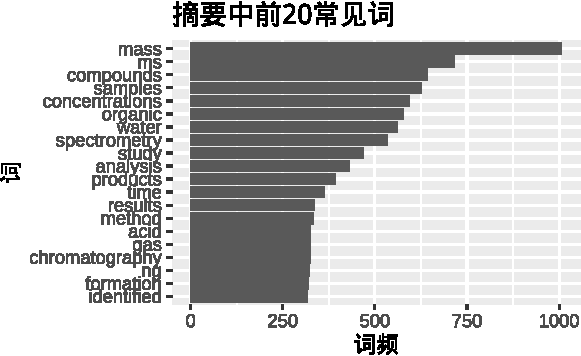
\includegraphics{sciguide_files/figure-latex/unnamed-chunk-34-1}

我们找到了822篇文献,从词频前20的结果看浓度、水、产物、方法、色谱、鉴定等词出现频率比较高。同时我们可以看下这10年关键词的变化趋势。

\begin{Shaded}
\begin{Highlighting}[]
\NormalTok{papers\_per\_month }\OtherTok{\textless{}{-}}\NormalTok{ tmdf }\SpecialCharTok{\%\textgreater{}\%}
  \FunctionTok{group\_by}\NormalTok{(month) }\SpecialCharTok{\%\textgreater{}\%}
  \FunctionTok{summarize}\NormalTok{(}\AttributeTok{month\_total =} \FunctionTok{n}\NormalTok{())}
\CommentTok{\# 摘要中关键词}
\NormalTok{word\_month\_counts }\OtherTok{\textless{}{-}}\NormalTok{ wordfabs }\SpecialCharTok{\%\textgreater{}\%}
  \FunctionTok{filter}\NormalTok{(word\_total }\SpecialCharTok{\textgreater{}=} \DecValTok{100}\NormalTok{) }\SpecialCharTok{\%\textgreater{}\%}
  \FunctionTok{count}\NormalTok{(word, month) }\SpecialCharTok{\%\textgreater{}\%}
  \FunctionTok{complete}\NormalTok{(word, month, }\AttributeTok{fill =} \FunctionTok{list}\NormalTok{(}\AttributeTok{n =} \DecValTok{0}\NormalTok{)) }\SpecialCharTok{\%\textgreater{}\%}
  \FunctionTok{inner\_join}\NormalTok{(papers\_per\_month, }\AttributeTok{by =} \StringTok{"month"}\NormalTok{) }\SpecialCharTok{\%\textgreater{}\%}
  \FunctionTok{mutate}\NormalTok{(}\AttributeTok{percent =}\NormalTok{ n }\SpecialCharTok{/}\NormalTok{ month\_total) }\SpecialCharTok{\%\textgreater{}\%}
  \FunctionTok{mutate}\NormalTok{(}\AttributeTok{year =} \FunctionTok{year}\NormalTok{(month) }\SpecialCharTok{+} \FunctionTok{yday}\NormalTok{(month) }\SpecialCharTok{/} \DecValTok{365}\NormalTok{) }\SpecialCharTok{\%\textgreater{}\%}
        \FunctionTok{filter}\NormalTok{(percent}\SpecialCharTok{\textless{}}\DecValTok{1}\NormalTok{)}
\CommentTok{\# 计数数据广义二项回归}
\NormalTok{mod }\OtherTok{\textless{}{-}} \ErrorTok{\textasciitilde{}} \FunctionTok{glm}\NormalTok{(}\FunctionTok{cbind}\NormalTok{(n, month\_total }\SpecialCharTok{{-}}\NormalTok{ n) }\SpecialCharTok{\textasciitilde{}}\NormalTok{ year, ., }\AttributeTok{family =} \StringTok{"binomial"}\NormalTok{)}
\CommentTok{\# 计算斜率}
\NormalTok{slopes }\OtherTok{\textless{}{-}}\NormalTok{ word\_month\_counts }\SpecialCharTok{\%\textgreater{}\%}
  \FunctionTok{nest}\NormalTok{(}\SpecialCharTok{{-}}\NormalTok{word) }\SpecialCharTok{\%\textgreater{}\%}
  \FunctionTok{mutate}\NormalTok{(}\AttributeTok{model =} \FunctionTok{map}\NormalTok{(data, mod)) }\SpecialCharTok{\%\textgreater{}\%}
  \FunctionTok{mutate}\NormalTok{(}\AttributeTok{models =} \FunctionTok{map}\NormalTok{(model,tidy)) }\SpecialCharTok{\%\textgreater{}\%}
  \FunctionTok{unnest}\NormalTok{(}\AttributeTok{cols =} \FunctionTok{c}\NormalTok{(models)) }\SpecialCharTok{\%\textgreater{}\%}
  \FunctionTok{filter}\NormalTok{(term }\SpecialCharTok{==} \StringTok{"year"}\NormalTok{) }\SpecialCharTok{\%\textgreater{}\%}
  \FunctionTok{arrange}\NormalTok{(}\FunctionTok{desc}\NormalTok{(estimate))}
\end{Highlighting}
\end{Shaded}

\begin{verbatim}
## Warning: All elements of `...` must be named.
## Did you want `data = -word`?
\end{verbatim}

\begin{Shaded}
\begin{Highlighting}[]
\CommentTok{\# 快速成长关键词}
\NormalTok{slopes }\SpecialCharTok{\%\textgreater{}\%}
  \FunctionTok{head}\NormalTok{(}\DecValTok{9}\NormalTok{) }\SpecialCharTok{\%\textgreater{}\%}
  \FunctionTok{inner\_join}\NormalTok{(word\_month\_counts, }\AttributeTok{by =} \StringTok{"word"}\NormalTok{) }\SpecialCharTok{\%\textgreater{}\%}
  \FunctionTok{mutate}\NormalTok{(}\AttributeTok{word =} \FunctionTok{reorder}\NormalTok{(word, }\SpecialCharTok{{-}}\NormalTok{estimate)) }\SpecialCharTok{\%\textgreater{}\%}
  \FunctionTok{ggplot}\NormalTok{(}\FunctionTok{aes}\NormalTok{(month, n }\SpecialCharTok{/}\NormalTok{ month\_total, }\AttributeTok{color =}\NormalTok{ word)) }\SpecialCharTok{+}
  \FunctionTok{geom\_line}\NormalTok{(}\AttributeTok{show.legend =} \ConstantTok{FALSE}\NormalTok{) }\SpecialCharTok{+}
  \FunctionTok{scale\_y\_continuous}\NormalTok{(}\AttributeTok{labels =} \FunctionTok{percent\_format}\NormalTok{()) }\SpecialCharTok{+}
  \FunctionTok{facet\_wrap}\NormalTok{(}\SpecialCharTok{\textasciitilde{}}\NormalTok{ word, }\AttributeTok{scales =} \StringTok{"free\_y"}\NormalTok{) }\SpecialCharTok{+}
  \FunctionTok{expand\_limits}\NormalTok{(}\AttributeTok{y =} \DecValTok{0}\NormalTok{) }\SpecialCharTok{+}
  \FunctionTok{labs}\NormalTok{(}\AttributeTok{x =} \StringTok{"年份"}\NormalTok{,}
       \AttributeTok{y =} \StringTok{"摘要中含有该关键词的百分比"}\NormalTok{,}
       \AttributeTok{title =} \StringTok{"增长率最快的9个词"}
\NormalTok{              )}
\end{Highlighting}
\end{Shaded}

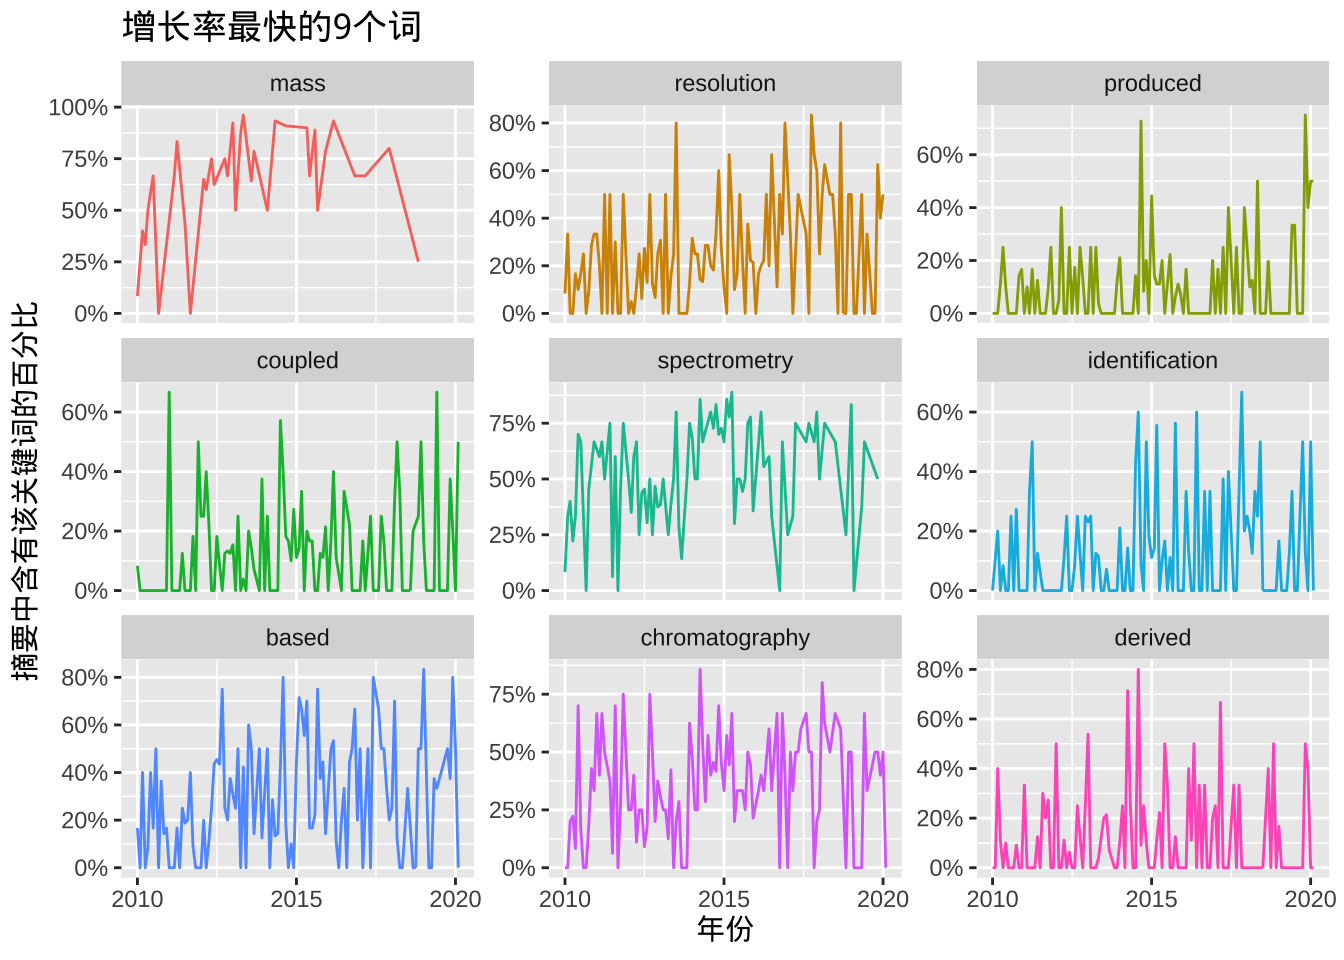
\includegraphics{sciguide_files/figure-latex/unnamed-chunk-35-1}

这里我们看到分辨率跟液相色谱的使用词频在逐渐上升。那么相应的我们也可以看下那些关键词在衰退。

\begin{Shaded}
\begin{Highlighting}[]
\CommentTok{\# 衰退关键词}
\NormalTok{slopes }\SpecialCharTok{\%\textgreater{}\%}
  \FunctionTok{tail}\NormalTok{(}\DecValTok{9}\NormalTok{) }\SpecialCharTok{\%\textgreater{}\%}
  \FunctionTok{inner\_join}\NormalTok{(word\_month\_counts, }\AttributeTok{by =} \StringTok{"word"}\NormalTok{) }\SpecialCharTok{\%\textgreater{}\%}
  \FunctionTok{mutate}\NormalTok{(}\AttributeTok{word =} \FunctionTok{reorder}\NormalTok{(word, estimate)) }\SpecialCharTok{\%\textgreater{}\%}
  \FunctionTok{ggplot}\NormalTok{(}\FunctionTok{aes}\NormalTok{(month, n }\SpecialCharTok{/}\NormalTok{ month\_total, }\AttributeTok{color =}\NormalTok{ word)) }\SpecialCharTok{+}
  \FunctionTok{geom\_line}\NormalTok{(}\AttributeTok{show.legend =} \ConstantTok{FALSE}\NormalTok{) }\SpecialCharTok{+}
  \FunctionTok{scale\_y\_continuous}\NormalTok{(}\AttributeTok{labels =} \FunctionTok{percent\_format}\NormalTok{()) }\SpecialCharTok{+}
  \FunctionTok{facet\_wrap}\NormalTok{(}\SpecialCharTok{\textasciitilde{}}\NormalTok{ word, }\AttributeTok{scales =} \StringTok{"free\_y"}\NormalTok{) }\SpecialCharTok{+}
  \FunctionTok{expand\_limits}\NormalTok{(}\AttributeTok{y =} \DecValTok{0}\NormalTok{) }\SpecialCharTok{+}
  \FunctionTok{labs}\NormalTok{(}\AttributeTok{x =} \StringTok{"年份"}\NormalTok{,}
       \AttributeTok{y =} \StringTok{"摘要中含有该关键词的百分比"}\NormalTok{,}
       \AttributeTok{title =} \StringTok{"衰退最快的9个词"}
\NormalTok{              )}
\end{Highlighting}
\end{Shaded}

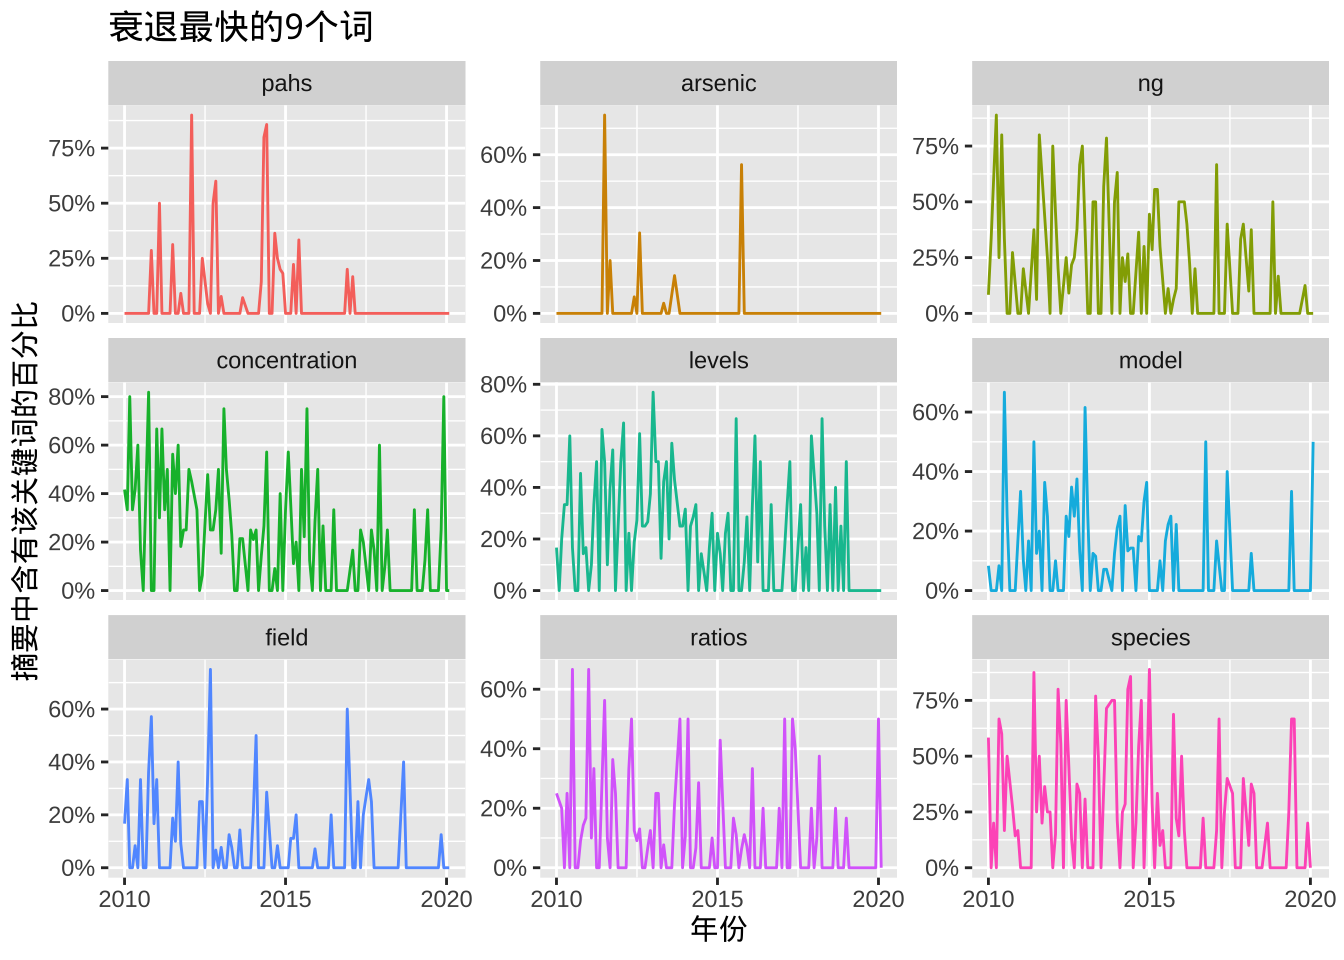
\includegraphics{sciguide_files/figure-latex/unnamed-chunk-36-1}

这里可以看到PAHs、砷、芳香族、酸等词在质谱相关的环境研究中逐渐减少。同时,我们也可以利用词频相关来研究关键词聚类情况。

\begin{Shaded}
\begin{Highlighting}[]
\FunctionTok{library}\NormalTok{(widyr)}
\FunctionTok{library}\NormalTok{(igraph)}
\FunctionTok{library}\NormalTok{(ggraph)}
\CommentTok{\# 计算两个词同时出现在摘要的频率,词频用边的宽度来表示}
\NormalTok{word\_pairs }\OtherTok{\textless{}{-}}\NormalTok{ wordfabs }\SpecialCharTok{\%\textgreater{}\%}
        \FunctionTok{pairwise\_count}\NormalTok{(word,line,}\AttributeTok{sort =} \ConstantTok{TRUE}\NormalTok{)}
\end{Highlighting}
\end{Shaded}

\begin{verbatim}
## Warning: `distinct_()` was deprecated in dplyr 0.7.0.
## Please use `distinct()` instead.
## See vignette('programming') for more help
## This warning is displayed once every 8 hours.
## Call `lifecycle::last_lifecycle_warnings()` to see where this warning was generated.
\end{verbatim}

\begin{Shaded}
\begin{Highlighting}[]
\FunctionTok{set.seed}\NormalTok{(}\DecValTok{42}\NormalTok{)}
\NormalTok{word\_pairs }\SpecialCharTok{\%\textgreater{}\%}
  \FunctionTok{filter}\NormalTok{(n }\SpecialCharTok{\textgreater{}=} \DecValTok{150}\NormalTok{) }\SpecialCharTok{\%\textgreater{}\%}
  \FunctionTok{graph\_from\_data\_frame}\NormalTok{() }\SpecialCharTok{\%\textgreater{}\%}
  \FunctionTok{ggraph}\NormalTok{(}\AttributeTok{layout =} \StringTok{"fr"}\NormalTok{) }\SpecialCharTok{+}
  \FunctionTok{geom\_edge\_link}\NormalTok{(}\FunctionTok{aes}\NormalTok{(}\AttributeTok{edge\_alpha =}\NormalTok{ n, }\AttributeTok{edge\_width =}\NormalTok{ n), }\AttributeTok{edge\_colour =} \StringTok{"cyan4"}\NormalTok{) }\SpecialCharTok{+}
  \FunctionTok{geom\_node\_point}\NormalTok{(}\AttributeTok{size =} \DecValTok{1}\NormalTok{) }\SpecialCharTok{+}
  \FunctionTok{geom\_node\_text}\NormalTok{(}\FunctionTok{aes}\NormalTok{(}\AttributeTok{label =}\NormalTok{ name), }\AttributeTok{repel =} \ConstantTok{TRUE}\NormalTok{, }
                 \AttributeTok{point.padding =} \FunctionTok{unit}\NormalTok{(}\FloatTok{0.2}\NormalTok{, }\StringTok{"lines"}\NormalTok{)) }\SpecialCharTok{+}
  \FunctionTok{labs}\NormalTok{(}\AttributeTok{title =} \StringTok{"摘要中的词对(Bigrams)"}\NormalTok{) }\SpecialCharTok{+}
  \FunctionTok{theme\_void}\NormalTok{()}
\end{Highlighting}
\end{Shaded}

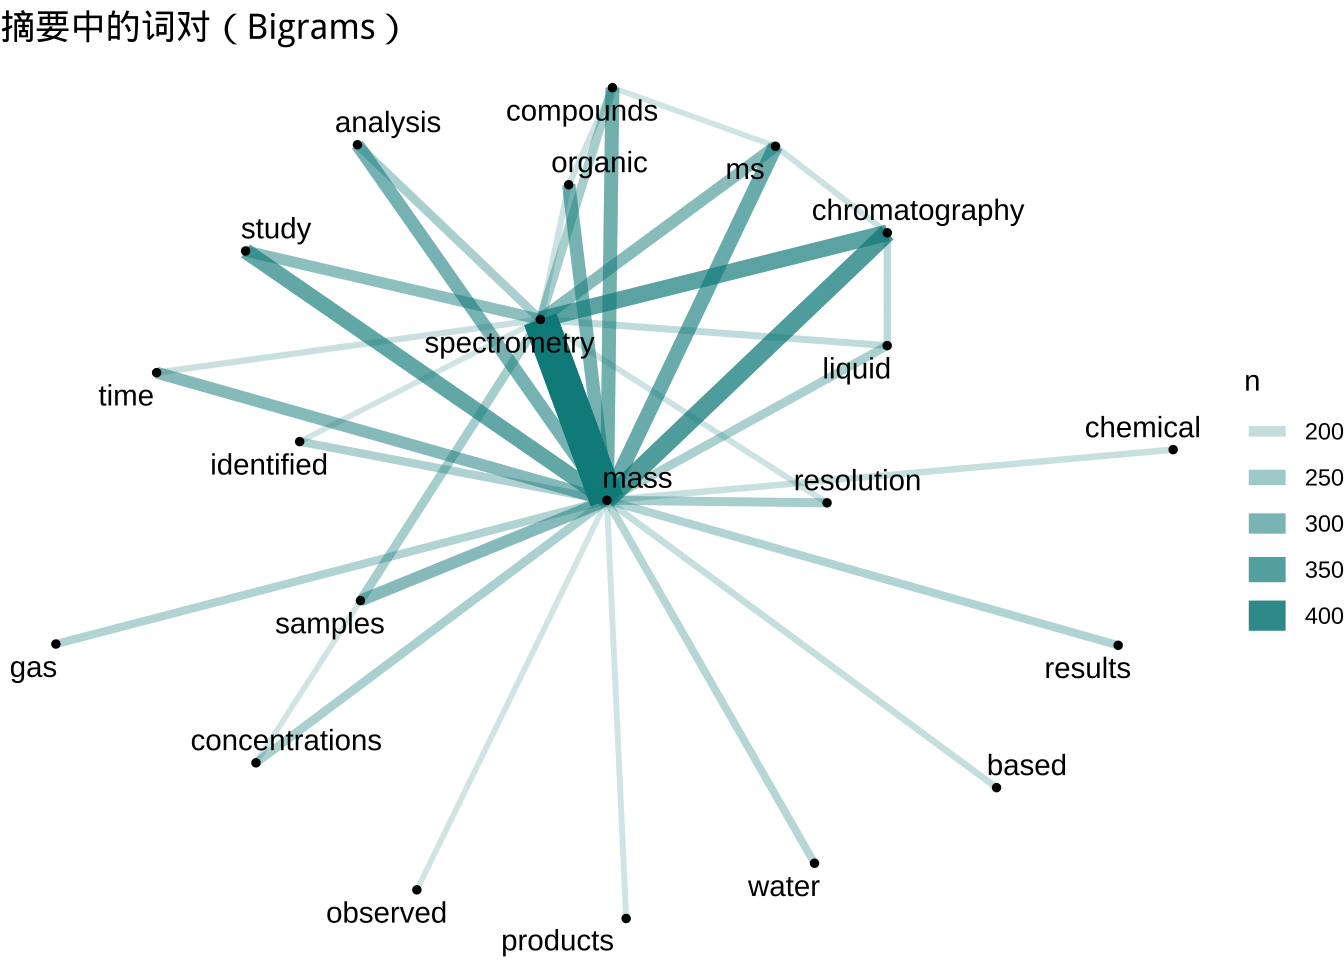
\includegraphics{sciguide_files/figure-latex/unnamed-chunk-37-1}

这样我们就直接生成了质谱环境应用的关键词网络。当然,更直接的方法是用主题模型来寻找子领域,例如我们可以指定6个子领域输出其前10关键词。

\begin{Shaded}
\begin{Highlighting}[]
\NormalTok{desc\_dtm }\OtherTok{\textless{}{-}}\NormalTok{ wordfabs }\SpecialCharTok{\%\textgreater{}\%}
        \FunctionTok{count}\NormalTok{(line, word, }\AttributeTok{sort =} \ConstantTok{TRUE}\NormalTok{) }\SpecialCharTok{\%\textgreater{}\%}
        \FunctionTok{ungroup}\NormalTok{() }\SpecialCharTok{\%\textgreater{}\%}
        \FunctionTok{cast\_dtm}\NormalTok{(line, word, n)}

\FunctionTok{library}\NormalTok{(topicmodels)}
\CommentTok{\# 潜在狄利克雷分布模型寻找6个潜在的子领域}
\NormalTok{desc\_lda }\OtherTok{\textless{}{-}} \FunctionTok{LDA}\NormalTok{(desc\_dtm, }\AttributeTok{k =} \DecValTok{6}\NormalTok{, }\AttributeTok{control =} \FunctionTok{list}\NormalTok{(}\AttributeTok{seed =} \DecValTok{42}\NormalTok{))}
\NormalTok{tidy\_lda }\OtherTok{\textless{}{-}} \FunctionTok{tidy}\NormalTok{(desc\_lda)}

\NormalTok{top\_terms }\OtherTok{\textless{}{-}}\NormalTok{ tidy\_lda }\SpecialCharTok{\%\textgreater{}\%}
  \FunctionTok{group\_by}\NormalTok{(topic) }\SpecialCharTok{\%\textgreater{}\%}
  \FunctionTok{top\_n}\NormalTok{(}\DecValTok{10}\NormalTok{, beta) }\SpecialCharTok{\%\textgreater{}\%}
  \FunctionTok{ungroup}\NormalTok{() }\SpecialCharTok{\%\textgreater{}\%}
  \FunctionTok{arrange}\NormalTok{(topic, }\SpecialCharTok{{-}}\NormalTok{beta)}

\NormalTok{top\_terms }\SpecialCharTok{\%\textgreater{}\%}
  \FunctionTok{mutate}\NormalTok{(}\AttributeTok{term =} \FunctionTok{reorder}\NormalTok{(term, beta)) }\SpecialCharTok{\%\textgreater{}\%}
  \FunctionTok{group\_by}\NormalTok{(topic, term) }\SpecialCharTok{\%\textgreater{}\%}    
  \FunctionTok{arrange}\NormalTok{(}\FunctionTok{desc}\NormalTok{(beta)) }\SpecialCharTok{\%\textgreater{}\%}  
  \FunctionTok{ungroup}\NormalTok{() }\SpecialCharTok{\%\textgreater{}\%}
  \FunctionTok{mutate}\NormalTok{(}\AttributeTok{term =} \FunctionTok{factor}\NormalTok{(}\FunctionTok{paste}\NormalTok{(term, topic, }\AttributeTok{sep =} \StringTok{"\_\_"}\NormalTok{), }
                       \AttributeTok{levels =} \FunctionTok{rev}\NormalTok{(}\FunctionTok{paste}\NormalTok{(term, topic, }\AttributeTok{sep =} \StringTok{"\_\_"}\NormalTok{)))) }\SpecialCharTok{\%\textgreater{}\%}
  \FunctionTok{ggplot}\NormalTok{(}\FunctionTok{aes}\NormalTok{(term, beta, }\AttributeTok{fill =} \FunctionTok{as.factor}\NormalTok{(topic))) }\SpecialCharTok{+}
  \FunctionTok{geom\_col}\NormalTok{(}\AttributeTok{show.legend =} \ConstantTok{FALSE}\NormalTok{) }\SpecialCharTok{+}
  \FunctionTok{coord\_flip}\NormalTok{() }\SpecialCharTok{+}
  \FunctionTok{scale\_x\_discrete}\NormalTok{(}\AttributeTok{labels =} \ControlFlowTok{function}\NormalTok{(x) }\FunctionTok{gsub}\NormalTok{(}\StringTok{"\_\_.+$"}\NormalTok{, }\StringTok{""}\NormalTok{, x)) }\SpecialCharTok{+}
  \FunctionTok{labs}\NormalTok{(}\AttributeTok{title =} \StringTok{"6个子领域主题的前10关键词"}\NormalTok{,}
       \AttributeTok{x =} \ConstantTok{NULL}\NormalTok{, }\AttributeTok{y =} \FunctionTok{expression}\NormalTok{(beta)) }\SpecialCharTok{+}
  \FunctionTok{facet\_wrap}\NormalTok{(}\SpecialCharTok{\textasciitilde{}}\NormalTok{ topic, }\AttributeTok{ncol =} \DecValTok{2}\NormalTok{, }\AttributeTok{scales =} \StringTok{"free"}\NormalTok{)}
\end{Highlighting}
\end{Shaded}

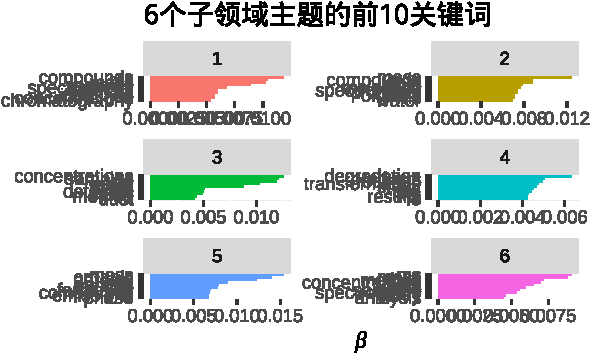
\includegraphics{sciguide_files/figure-latex/unnamed-chunk-38-1}

主题模型会尝试将相关性高的词归为一个主题,这里我们大体可以推测出第一个主题是关于气相色谱物质鉴定的;第二个主题是关于水中天然溶解性有机物分析;第三个大概是水样灰尘样中污染物定量研究;第四个大概是土壤降解转化产物;第五个是气溶胶反应产物;第六个则是水样的分析方法研究。这样,通过文本挖掘我们就可以推测出一些通常需要阅读很多文献才能形成的学科发展趋势。

\hypertarget{ux4f5cux8005}{%
\subsection{作者}\label{ux4f5cux8005}}

同样的,我们也可以研究某个作者的研究主题与变化趋势。下面是获取加拿大滑铁卢大学 Jaunsz Pawliszyn 教授的数据的代码,其数据分析部分与前一章节关键词相同。

\begin{Shaded}
\begin{Highlighting}[]
\CommentTok{\# 10年跨度}
\NormalTok{query }\OtherTok{\textless{}{-}} \StringTok{\textquotesingle{}janusz pawliszyn[AU] AND 2010/01:2020/01[DP]\textquotesingle{}}
\NormalTok{tmdf }\OtherTok{\textless{}{-}} \FunctionTok{getpubmed}\NormalTok{(query, }\AttributeTok{start =} \DecValTok{1}\NormalTok{, }\AttributeTok{end =} \DecValTok{10000}\NormalTok{) }\SpecialCharTok{\%\textgreater{}\%}
        \FunctionTok{getpubmedtbl}\NormalTok{() }\SpecialCharTok{\%\textgreater{}\%}
        \FunctionTok{mutate}\NormalTok{(}\AttributeTok{time =} \FunctionTok{as.POSIXct}\NormalTok{(date, }\AttributeTok{origin =} \StringTok{"1970{-}01{-}01"}\NormalTok{),}
         \AttributeTok{month =} \FunctionTok{round\_date}\NormalTok{(date, }\StringTok{"month"}\NormalTok{))}
\end{Highlighting}
\end{Shaded}

\begin{verbatim}
## 195 records founds
\end{verbatim}

此外,我们用下面代码输出其发表学术期刊的偏好。

\begin{Shaded}
\begin{Highlighting}[]
\CommentTok{\# 给出发表数前10的期刊}
\FunctionTok{table}\NormalTok{(tmdf}\SpecialCharTok{$}\NormalTok{journal)[}\FunctionTok{order}\NormalTok{(}\FunctionTok{table}\NormalTok{(tmdf}\SpecialCharTok{$}\NormalTok{journal),}\AttributeTok{decreasing =}\NormalTok{ T)][}\DecValTok{1}\SpecialCharTok{:}\DecValTok{10}\NormalTok{]   }
\end{Highlighting}
\end{Shaded}

\begin{verbatim}
## 
##              Anal Chem         Anal Chim Acta         J Chromatogr A 
##                     44                     33                     32 
##            Bioanalysis    Environ Sci Technol              J Sep Sci 
##                      9                      7                      7 
## Angew Chem Int Ed Engl                Sci Rep                Talanta 
##                      6                      6                      6 
##                Analyst 
##                      4
\end{verbatim}

\hypertarget{ux5168ux5b66ux79d1ux8bc4ux4ef7}{%
\section{全学科评价}\label{ux5168ux5b66ux79d1ux8bc4ux4ef7}}

除了了解本学科知识,我们还要知道本学科在所有学科中的分量。虽然很多人批评文章数量不代表学科热度,但我觉得起码每篇论文都在解决一个科学问题,所以这里的比较就统一用文章数量。为了进一步简化评价,我们这里就用 PubMed 数据库的结果来说明,也就是说探索的是生物医药领域内不同研究领域的发展状况。方法也极为简单,就是关键词搜索。下面这个过程大家可以自行验证,其实用 Web of Science 更合理。

首先要了解自己的信息处理能力。我自己追踪的学科内紧密相关研究一年发文量不超过 100,也就是一个周一两篇的样子。这个知识更新频率应该是比较符合科研人员个体信息处理能力的。如果你关注的领域非常热,发文量很高,那么大概率你也会自主把文献查新的量通过关键词叠加来缩小到一周一两篇,大概一季度甚至一年出现一篇小领域综述的状态。而且这个量我觉得对大多数科研人员还是超载了,很多研究人员的研究方向非常精细,一年内同行发文量个位数,全世界也就几个课题组在做。那么此时应适当眼界放宽些,否则你的研究会被视野限制住。

当一个关键词年同行发文数量超过一百时,围绕这个关键词的全国性年会就会召开,也可能会拥有自己的专业期刊与学会,小型国际会议也可以组建了,例如纳米毒理学或持久性有机污染物。这个状态下的学科要么快速发展,要么快速衰退,全球相关课题组数量不会超过三位数,这类学科一年内如果频繁登上 CNS(Cell, Nature, Science)等综合性期刊,那么很可能进入指数增长期,但如果一年内一篇都没有,那消退也很快。如果低于这个量,那么关键词对应研究组可能还从属于某个大学科,属于大课题下的边缘课题,绝大多数退学的博士生都是挂在这类几乎看不到发展希望的项目上了。顺带一提,国内的杰青级评选的候选人至少要在国内是这个量级领域下的数一数二的人物,这样的领域整体看大概 1000 个左右。

当年同行发文量超过两千时,千人级国际性会议就能开,开的不错,行业内会出现多份期刊来吸纳不同层次的论文。而且我观察超过一千后的研究领域很少有萎缩的,但这是第一个停滞点,很多领域的规模上限就是两千。从人才角度看,国内在这个量级上数一数二的人物都是院士级的。这样的关键词例如纳米银、生物医药里的深度学习,这个量级如果能保持增长,那绝对会是学科热点,估计对应从业人员超过一万了,这类学科基本都有产业化的课题做支撑了。

年同行发文量在两千到一万的学科是非常多的,这是通常意义上的的科研方向,例如代谢组学、精准医疗这类。这类研究你应该能从公众报道到听到了,全球有四位数的课题组,基本每所综合类大学都有至少一个人在从事相关研究。国家重点实验室基本都是在这个量级上构建的,企业也会有研发团队,且这个量级的实际需求已经有行业级支撑。

超过一万的关键词都可以称得上前沿或热点学科并且已经有能力渗透到其他学科了,例如纳米颗粒、基因组学、分析化学、睡眠、衰老等。每天科技新闻都会有相关报道,是 CNS 的常客。相关创业公司会受到科技类风投的重点关注。然而这里会遇到第二个停滞点,实际上这个量级的研究已经是此消彼长的发文量了,相互之间会有学科级资源分配问题,在国家层面会出政策来扶植这个量级学科的成长,当然如果财政有限,拿来支持的资源必然是其他学科抽的。这个级别是可能萎缩的,例如同位素研究在上世纪六七十年代曾经接近两万,但现在稳定在四五千的体量,这就是撞了停滞点了。

然而,还有一些顶级关键词。生物医药科研里的顶级研究领域是细胞,最近三年年发文量稳定在30万的样子。然后是癌症,这个关键词最近三年基本稳定在20万。研究血液的在 15 年达到顶峰,发文量约18万。脑类相关研究在约10万的发文量。另一种热点疾病的是心脑血管疾病,在不到10万的年发文量。顶级研究热点一般要发文量超过5万,但似乎不会超过 30万。

几乎每一个顶级研究领域都有一堆下属子学科,子学科的国际会议都能达到几千人级别。这些关键词几乎都配备国家实验室或研究所,数量每个国家也就十几个。这类学科已经不是渗透其他学科发展了,更多是引导性发展,这个领域出现的方法学进步会直接超越其他领域,也能吸引到很多超精英,带动整体进步。诺奖应该就是这个量级关键词上的进步的后果。

这里我简单分个级(按幽游白书的分级方法):

\begin{itemize}
\tightlist
\item
  S级 年同行发文量超过 5 万的关键词领域,疑似有停滞点
\item
  A级 年同行发文量 1 万到 5 万的关键词领域,有停滞点
\item
  B级 年同行发文量 2 千到 1 万的关键词领域,有停滞点
\item
  C级 年同行发文量 100 到 2 千的关键词领域
\item
  D级及以下 年同行发文量 100 以下的关键词领域
\end{itemize}

这个应该就是大多数科研人员的天梯系统了,研究在D级,关注到C级的研究动态,参与B级领域的会议,蹭A级的热点,然后远远看下S级开心就好。通过这种简单但可能不靠谱的分析,科研人员应该可以实现一个对自己的清楚定位,然后合理规划自己的视野,防止见树木不见森林,也防止迷失在过大的森林里。上世纪科研界花费了大量精力去构建术语体系与专业学科的墙,这个世纪我们该尝试打破这些意义不大的墙去解决一些复杂而现实的问题了。

\hypertarget{ux835fux8403ux5206ux6790}{%
\section{荟萃分析}\label{ux835fux8403ux5206ux6790}}

荟萃分析常用来对已发表的实验结果进行二次分析得到一个更全面的结论,常用于心理学、流行病学与经济学研究等。其应用场景通常是想回答一个被重复研究过的科学问题,例如某种疾病在不同人群中的风险比等。不过,不同实验精度不同、样本量不同、方差不同、效应也会不同,此时荟萃分析就可以用来汇总出一个关于结论的结论,本质上是一个层级模型。

荟萃分析有两种基本模型,一种是固定效应模型,一种是随机效应模型。前者只有确认不同研究都针对同一群体时才适合用,然而绝大多数情况下不同研究的群体是不一样的,因此实际使用中随机效应模型用的更多,因为其考虑了不同研究自身的随机性。

固定效应模型对总效应的估计是基于对不同研究方差的倒数加权来计算的,也就是说研究的标准误越高,其对总效应的贡献就越小,具体公式是:

\[\hat\theta_F = \frac{\sum\limits_{k=1}^K \hat\theta_k/ \hat\sigma^2_k}{\sum\limits_{k=1}^K 1/\hat\sigma^2_k}\]

如果样本存在异质性,那么就要用随机效应模型。在随机效应模型中,我们假设每一研究给出的效应来自于一个分布而不是固定的值,这样我们就还要估计这个分布的不确定度,一般用 \(\tau^2\) 来表示。同时,效应可以是连续变量,也可以是二元变量,也可以是类似相关系数的统计量。

荟萃分析的结果通常用森林图来表示,上面会列上单独研究的效应估计及置信区间、权重,也会给出整体效应估计与置信区间。同时,一般荟萃分析的软件也会给出异质性系数及对该系数的假设检验结果,也会给出预测区间。如果异质性系数低于 25\% ,我们会认为可以直接用固定效应模型,如果高于75\%,则异质性非常大。预测区间给出的是基于当前荟萃分析结果未来研究效应可能出现的区间,通常比估计效应的置信区间要大,但回答的不是一个问题,估计效应的置信区间描述得是多次重复实验后在一定置信水平下真值会出现的区间。

在荟萃分析中,有些个别研究可能对整体估计产生较大影响,所以要进行敏感度分析或影响分析,通常敏感度分析是用留一法来做的,也就是排除掉这个研究去重新估计效应,看前后差距是否显著,如果显著最好排除掉。

有时荟萃分析中研究可以进一步分类,此时可以引入混合效应模型,也就是各分类效应固定,但各分类效应的误差来自于一个分布。同时研究中涉及的变量如果不是分类而是连续变量,那么也可以进行荟萃回归分析,同样可以做固定效应模型与混合效应模型。

荟萃分析中一个重要主题就是发表歧视,小样本研究通常可信度要低于大样本但容易获得明显效应。漏斗图常用来表示不同效应及标准误的汇聚程度,根据对称性检验(Egger's test)我们可以推测哪些研究结果可能存在发表歧视。另一种发表歧视的检验方法是汇总分析 p 值的分布,如果真实效应存在则应该是左偏的,而不是汇聚到 0.05 附近。

荟萃分析还可以进一步通过对研究质量进行定量后汇总评价,主要用来展示不同操作步骤引入的不确定性。更为复杂的荟萃分析会去考虑不同处理间的直接与间接影响,一般是通过网络分析来进行。同理,这类存在层级结构的分析问题也可以通过结构方程模型来求解,寻找出观察层背后的潜在结构。

\hypertarget{life}{%
\chapter{学术生活}\label{life}}

现代科研会影响渗透到科研人员的日常生活之中,本章会讨论下学术生活中一些重要的议题。学术道德与伦理是第一位的,在职业化的科研中有一票否决的权力。邮件是最常见的学术交流工具,我们会讨论下一些基本礼仪。学术出版、学术会议与审稿则是最正式的学术交流方式,我们会讨论下其中的注意事项。之后会讨论下学术合作的问题与利益冲突问题。课题组管理可能是现代科研行业里最容易忽视的一环,这里会介绍下课题组管理的注意事项。最后,讲课也是学术生活的重要组成部分,需要普及一些基本的教学理念或方法。

\hypertarget{ux5b66ux672fux9053ux5fb7ux4f26ux7406}{%
\section{学术道德/伦理}\label{ux5b66ux672fux9053ux5fb7ux4f26ux7406}}

学术道德与伦理经常是默认科研人员都知道但其实新闻的教育效果要大于课堂教育的论题。这里从剽窃、文章挂名、双重发表、数据造假、有害研究实践、合规性、性骚扰及伦理方面来介绍下相关内容。

\hypertarget{ux527dux7a83}{%
\subsection{剽窃}\label{ux527dux7a83}}

剽窃(plagiarism)包括但不限于对他人发表或未发表工作、想法、数据等的不恰当引用或故意不引用,也包括对自己发表成果的重复使用。在引述别人观点时,要做到总结转述与引用同时使用以表示对原作者的致敬。整段引用可使用引号但要根据期刊要求来做,转述不能简单做语序调整与同义词互换,要做到理解层面的叙述。对于别人在学术交流场合进行的讨论,也要进行充分引用来说明来源,学术圈里人们不会因为想法是你的而尊敬你多少,但会因为想法不是你的你却说成是自己的而鄙视你。

\hypertarget{ux6587ux7ae0ux6302ux540d}{%
\subsection{文章挂名}\label{ux6587ux7ae0ux6302ux540d}}

尽早决定且只有对文章有显著智力非物质贡献的人适合挂名,在现实中会存在索要挂名的行为但需要综合考虑。一般来说,挂名作者要至少有如下行为之一:

\begin{itemize}
\tightlist
\item
  提出概念或设计
\item
  收集分析数据
\item
  撰写草稿
\item
  同意最终版本发表并负责
\end{itemize}

不得不承认的是有些人可能仅仅是在文章写作阶段参与,但其对文章的内容理解阐述可以让读者很简单了解文章的内容,此时是否列入作者需要综合考虑而不是单纯排斥,每篇文章都有自己的生命力而不是私产。当然请编辑润稿不在其中,因为编辑不对内容负责。影子作者或者代笔是严格禁止的。对于吉祥物作者,请知会该作者并阐明挂名风险,能成为吉祥物的资深研究人员有能力对自己的名誉风险做判断。各个领域的要求可能不同,但很简单的方法就是文章列一个作者贡献章节,详细记录每个挂名作者的贡献。

除了挂名,致谢中表示物质援助与技术援助也是一种不错的致敬方式,在感谢前,请告知他们并获取同意许可。

文章挂名的另一个问题是作者排序,常规操作是资深研究人员放在最后,第一作者是文章主要撰写人。作者排序常常由资深研究人员来决定,因为他们对全局智力贡献把握更准确,但最好做到内部透明。如果智力贡献不多,做实验最多的人有可能不被列为第一作者,对于研究生而言,请不要把体力劳动当成第一作者的保险,请一定参与数据分析与文章撰写磨练自己的科研能力。有些领域例如物理学会按字母表来进行作者排序,但并未广泛推广。个人认为比较理性的情况是作者字母排序配合致谢与贡献章节来解决挂名问题。

\hypertarget{ux53ccux91cdux53d1ux8868}{%
\subsection{双重发表}\label{ux53ccux91cdux53d1ux8868}}

一稿两投严格禁止,这对同行评议期刊的自愿审稿资源是浪费,也是不尊重。但双重发表在以下情况可能是允许的:

\begin{itemize}
\tightlist
\item
  翻译
\item
  在选集中发表
\item
  文章受众不同
\item
  期刊间交流透明并对著作权无异议
\end{itemize}

\hypertarget{ux6570ux636eux9020ux5047}{%
\subsection{数据造假}\label{ux6570ux636eux9020ux5047}}

伪造(fabrication)是通过创造数据来论证自己想要的答案。修改图片,用仿真数据充当真实数据等方式都属于伪造。伪造可通过统计手段或其他技术手段来检验,两个检验原则是1)真实数据不太可能是完美的与2)假的数据比真数据更有目的性。

篡改(falsification)是通过对真实数据进行修改来论证自己想要的答案。这种比单纯伪造要难发现,但独立实验室验证会发现问题。篡改数据可以从制度上来规避,例如原始数据第一时间备份及保留数据处理软件的日志等。

\hypertarget{ux6709ux5bb3ux7814ux7a76ux5b9eux8df5}{%
\subsection{有害研究实践}\label{ux6709ux5bb3ux7814ux7a76ux5b9eux8df5}}

有害研究实践(detrimental research practices)指的是一些不易界定的学术不端,例如使用错误的统计方法与实验设计,故意隐瞒阴性结果及不披露利益冲突等手段。针对有害研究实践目前并没有很好的应对方法,但可以从基金资助角度要求研究的透明度,除了论文也要公开相关报告。

\hypertarget{ux5408ux89c4ux6027}{%
\subsection{合规性}\label{ux5408ux89c4ux6027}}

不合规(Noncompliance)指的是违法政策法规的研究,通常涉及伦理问题。合规性具备文化差异,确实有些研究在某些国家不容易开展而另一些国家则限制不多,这些在跨文化学术交流时一定要注意。

\hypertarget{ux6027ux9a9aux6270}{%
\subsection{性骚扰}\label{ux6027ux9a9aux6270}}

学术界性骚扰也是学术不端的一种形式,除了道德法律政策不允许外还会直接影响实验可信度。性骚扰包含异性与同性间涉及使用显性或隐性的性暗示的骚扰。性骚扰不仅仅包括行为上骚扰,通过口头欺辱、威胁或承诺换取性好处也属于性骚扰。

研究场合如果遇到性骚扰请上报,绝大多数公司或研究机构都会有专门负责的部门例如人事部门、妇联或工会来处理相关问题。鉴于报导出的性骚扰只占真实发生的性骚扰事件的一小部分,查实后一般都是从严处理行为不当的人。

\hypertarget{ux6b67ux89c6}{%
\subsection{歧视}\label{ux6b67ux89c6}}

歧视很多时候属于经济问题。很多运动过后会有很多人口头上表示支持反歧视但行为上依然我行我素,这样的运动主要是忽视了歧视行为背后的利益。生活在移民国家或城市的人则主要存在先来的对后来的歧视,先来的人通常垄断了移民国家或城市的话语权与价值观,在经济与政治上占有优势。美国的白人清教徒对后来的黑奴就存在这种历史性歧视,但区分先来与后来人的不仅仅是种族,还可能是地域,例如历史上上海本地人就对从事相对底层工作的苏北人有过长时间的歧视。经济上既得利益集团会给自己找些有门槛的标签(例如种族、地域、信仰、性别、职业等)来维护自己的利益并合理化这些歧视行为,常见的借口就是遗传差异或生理差异,但这些说辞并不被科学研究支持。现代社会的机器化大生产也基本抹平了很多职业的生理差异,但总会有人使用这些过时且迂腐的观点来为自己的歧视行为辩护。即使是生活在单一民族国家或城市的人也会因为一些文化民俗产生一些标签化偏见,落实为行为也属于歧视。例如招聘过程中对血型、星座、生肖、外貌等的偏好。现代社会中会不断生成新的歧视标签,因此反歧视的努力也不能间断。

学术界也存在歧视,不过很多人无法意识到自己的言语与行为对别人是一种歧视。有些科研人员会在招生时歧视学历与性别,但说到底都是为了维护自己利益最大化并确保课题组风险最小化。要抵制歧视行为,指望个人高风亮节的效果很差,应该构建兼顾机会公平的体制。不过,绝对的公平过于理想,甚至不同人立场不同对公平的理解也不一样。以性别歧视而言,利益受损的性别会去主张不公平的受损待遇但却会忽视自己已经受益的待遇,这样的主张会让另一方感觉无理取闹,等双方都带着情绪立场来辩论必然谁也说服不了谁,最后歧视问题没解决反而加重了人群分裂与对立。一旦出现一方要坚决打倒另一方且双方互相指责歧视,那么歧视就只是一个发泄情绪的借口而不是可以解决的问题了。

歧视问题必然与社会发展长期共存且不断发展,经常是一类歧视伴随发展消失但又出现了另一类歧视,反对歧视的核心应该是换位思考而不是抓紧区分敌我后发泄情绪。任何只取悦部分人利益的所谓反歧视解决方案必然会被另一部分人抵制,临时疏导双方情绪并不能真正解决问题,调和利益达成共识才有可能消除歧视根源。当然,这句在很多事实面前属于正确但无用的废话。

\hypertarget{ux4f26ux7406}{%
\subsection{伦理}\label{ux4f26ux7406}}

广义科研伦理包括不限于正直(说话算数可信)、诚实(不弄虚作假)、透明(可披露研究非隐私细节)、能力(专业性)、合作(能与人共事进行研究)、社会责任、服从法律法规公义与责任心。科研人员不能在伦理问题上出问题,否则会断送职业生涯。

此外,伦理问题更多是社会问题而不是科学问题,可以用科学方法来研究伦理问题但伦理问题不一定有明确的答案。歧视与偏见问题是科研中经常遇到的,同样的问题在不同的知识背景描述下会给第三方产生不适,此时要尽量采用中性描述而不是渲染情感。在交流时请尽量提前划定双方的底线,只讨论双方有讨论空间的问题而没必要在缺乏证据的基础上对观点发表意见。

\hypertarget{ux90aeux4ef6}{%
\section{邮件}\label{ux90aeux4ef6}}

邮件回复要快,工作日24小时以内,节假日不发邮件。题目要有辨识度,简明扼要,题目/正文要有关键词方便检索。一封邮件讨论一件事,简短,让读者有可操作性,给出决策问句。时间紧急时告诉收信人无回复的结果,有后续追踪。有附件一定在正文中说明。邮件签名提供自己联系方式。尽量用纯文本文件,开拼写检查。明白抄送的人没有回复义务,秘密抄送尽量不要用,注意回复一个人还是所有人。收到回信根据落款选择下一次名字,给陌生人邮件第一句介绍自己,第二句介绍你如何直到对方,不要用带有压迫性的 I wanted 或 I would like,用 I was wondering。可使用列表来分条目讲问题。避免用 please。结尾表示感谢,落款可用 Sincerely,Best wishes,Thanks。

\hypertarget{ux5b66ux672fux51faux7248}{%
\section{学术出版}\label{ux5b66ux672fux51faux7248}}

学术出版是学术工作的重头戏,期刊论文、会议摘要、专著、专利还有软件都属于学术出版的内容,下面将详细讨论这几类出版物的注意事项。

\hypertarget{ux671fux520aux8bbaux6587}{%
\subsection{期刊论文}\label{ux671fux520aux8bbaux6587}}

写论文的时间分配不是一个可以计划的东西,从一开始提出假设,设计实验,执行实验到数据分析,这些工作都不算在写论文的时间里,但这些阶段如果没有文献与实验结果的积累,最后的论文写作会变得无比痛苦。这里假设前期工作是比较理想的。

第一阶段是组织材料,这一阶段是最重要的,大概占论文写作70\%的时间。论文边写边找文献支持会很乱,所以同一时间就做一件事,那就需要先组织资料。而组织资料是要有一个分类系统,也就是说看到一篇文献,你脑中要能把它定位在你论文中出现的地方,例如前言或讨论。这里我建议尝试用一下思维导图,你的核心想法在中间,发散出例如背景,方法,类似研究等子话题,相当于使用树形目录组织文献。之后,你可以关上电脑,找张纸把你的写作大纲列出来,想出每一段的主题与结构。当你做完这些工作后,文章就剩下写这一个步骤了。这个过程可以贯穿到数据分析之前的所有步骤,因为脑子随时可以思考问题。

前一阶段如果做好了,写初稿并不困难,用10\%的时间。初稿不要一上来就力求完美,尽量按顺序吧想法说清楚,重点看逻辑,句型什么的可以放放,一气呵成,要马上动笔,拒绝完美。然后进入下一阶段,如果纠结写作细节会影响整体内容的思考,先把你的故事说出来,然后再润色。

之后的修改阶段可以多花时间,约20\%,主要针对表述。大声把论文读出来,看跟读是不一样的,能发现不少问题。检查动词的使用与语态的使用,其实上篇讲的东西就是为这个阶段准备的。然后你可以找一个同专业不同方向的同事读一下,因为你的文章更多被这些人读,所以他们能否读懂决定你的表达能力,读不明白一定就是你没写好,至于文章档次在你设计实验时基本就定型了。如果有条件的话最好找个专业编辑给你改改。感觉不会表述可以去查曼彻斯特大学的\href{https://www.phrasebank.manchester.ac.uk/}{Academic Phrasebank}来找模版句式,想换个同义词就到网上去搜索,一般而言你不会是第一个遇到这个问题的。

然后是检查阶段,就是查缺补漏,主要针对校对等最后期的工作。例如编号前后一致,参考文献的指代。这里要注意的是引用文献一定要看原文,转引不靠谱,因为很多发表的文章引用上并不见得没错误。

时间分配的核心在于细化步骤,理清思路,一段时间解决一个问题而不是同时解决表述、语法、引用等多方面的问题。优先考虑内容的表达,然后才是形式的修改,做到有条不紊,平稳写作。

一般的写作顺序为图表-\textgreater 结果-\textgreater 方法-\textgreater 前言-\textgreater 讨论-\textgreater 结论-\textgreater 摘要,内在的逻辑是当你实验数据处理完了,首先得到的就是分析数据的产品------图表,结果部分其实是围绕图表转的,所以这两部分趁热打铁最先完成。然后就是遵循由难到易的过程先把方法写了,这部分也不痛苦。然后就是前言,这部分就是小综述,文献看到位就可以写出来。最后的重头戏就是讨论,这部分最难写,逻辑要求最高,写完了结论与摘要就自然而然写出来了。按这个顺序你可以较为流畅的写完初稿。

在写文章上,图表是最直观也最应该先做出来的。你的工作浓缩在一张图里是最容易给人留下印象的,正所谓一图胜千言。对图表的要求则是要能独立的说明一个问题,而且越少越好。现在很多期刊要求有图形摘要其实就是方便读者快速抓住核心想法的,每一张图都尽可能漂亮且说明性强,不是单纯罗列数据而是尽可能展示数据的规律。

然后是结果,很多期刊是要求结果与讨论分离的,这个时候结果的目的就在于描述实验结果的现象。需要注意的是这个部分不等于描述原始数据,你需要在结果部分展示上面一步做好的图表并指出简单的关系与趋势。需要注意的是在图表中出现的数据除非特别重要就不要写出来了,图上不方便标明的数据在结果中要有交待。一定记得描述你的对照实验,让结果部分在逻辑上没有漏洞。此外,结果中提到的显著差异一定要是统计学上的而不是看出来的,也不要在结果里讨论方法与他人观点,这些内容有其他章节负责。结果就是描述你的实验结果,用过去式,但图表的解释用现在式。

之后是方法,这部分没什么好说的,实验设计要严谨表述。如果按文献方法做要引用出处,自己设计的最好给个流程图,不要让读者读着太痛苦。可用过去式与被动语态,统计方法记着要写清楚了。

之后是前言,这部分可以看作小综述,但实际写作也有其逻辑结构,一般写三段,按照已知-未知-假说的结构写。也就是说,写一下关于研究对象你知道什么,不知道什么,你提出的假设是什么。这样比较符合人们认识事物的过程且不乱,用语要高度概括,不要纠结于细节,那是写综述要注意的,这样从大到小收敛到你的工作上下面就可以讨论你的文章了。

之后的讨论这是最难写的部分,也是最自由的部分,与前言相反,这部分你要能把你的发现定位到大背景中。一般的逻辑结构是先回答你自己提出的假设的结果,然后用你的数据说明结果,之后广引文献来证明你的结果并讨论与其他研究结果不同的原因,也就是展开讨论未知,最后把你的结果定位到已知的位置看能否说明一些问题。值得注意的是不要过度演绎你的实验结果,也要讨论下局限性与前景。在这一部分你要着重使用上篇中提到的三个原则,结论强劲有力,不要遮遮掩掩,这些遮掩会让审稿人感觉你的结果不可靠且对学科发展没意义。

之后结论这一部分简短一点,把你文章的亮点展示出来就OK,同时可以用一句话做出展望。

最后写摘要,摘要部分其实就几句话,一句话说背景,一句话提出自己的假设或问题,一句话描述实验方法,一句话给出最核心结果,然后给出一句话结论并加上合理的推测。当然你也可以按照你自己的思路去写,但要记清楚,很多人看文章只看摘要的。把它放最后的意义也在于能够让你很好的去总结自己的文章。

目前很多期刊要求注明经费来源与个人贡献,很多还对数据共享与可视化有额外要求,请投稿时一定核查清楚。在论文挂名与致谢上,有实际贡献特别是论文修改与实验的智力贡献才可挂名,否则属于致谢。

写作顺序的考量其实就是一个从简单到复杂的考量,先处理简单的部分的优势在于如果你上来就去讨论,很可能脱离实际数据而瞻前顾后。

此外,论文写作也有一些其他的注意事项。首先,一定要注重精简,也就是写文章要有读者的视角。语言简洁可能不利于发表,但有利于传播。不考虑读者一味堆砌专业术语与高级句式,只会让人读不懂,在审稿人看来自然就是英文很烂的表现。高级句式与词汇是锦上添花的东西,没有通俗易懂的锦,只会让人看花眼。科技论文不代表就一定要从句套从句,这样的句子属于中国特色的阅读理解。老外(北美多于欧洲)都喜欢直来直去,论文表达内容优先,句式什么的可以放后面考虑。先看明白了再说别的,看不明白不是故意虚掩就是表意不清,一般审稿人会按后者对待写到审稿意见上。而且要有力度有自信的说出来,不去绕弯子。要是不习惯,可以先写成繁冗模式,然后精简。

常见的可精简词语:

\begin{itemize}
\tightlist
\item
  无意义引导词如As it is well known
\item
  空洞语句如basic tenets of
\item
  不必要的缩写与专用名词如 miR
\item
  重复性词语如illustrate/demonstrate
\item
  副词如very, really, quite, basically, generally, etc.
\end{itemize}

少用否定句。否定他人和自己都不是有自信的表现。少用there is/are。主语提前,要不然读者找起来费事,给读者找麻烦就是给自己找麻烦。不用没意义的介词。that跟on,读者会自己脑补的,在理解上有没有没区别就精简掉。

另外是可以使用主动语态的简单句的。被动语态会省略主语,显得不负责任。而使用主动语态会让文章更为生动真实,易于阅读且也是一种认真负责的态度。事实上越是高端的期刊越不计较这事,science就明确同意使用第一人称,而DNA被发现的那篇经典论文(发表于nature)的第一句也使用了第一人称。主动语态可以用在除方法描述外的任何场合,可间歇配合被动语态让文章更流畅。而实验方法的描述使用被动语态则是因为怎么做比谁做了更重要,同时关注方法部分的读者实际只关注一些关键词,写生动没多大意义。

使用强有力的动词。把中性动词+形容词改为动词,这样不罗嗦,少用to be,用了to be就可参照上面改成一个动词,简化句式。不要把动词改成动名词,可结合主动语态理解。主语跟动词要靠近,不要让读者找动词,不易于表意。在动词时态选择上,过去式描述自己的实验结果,一般式描述继承或验证过的事实与结论,未来式写展望。

标点符号也不仅仅用逗号与句号。分号用来表示一个句子的从句,有主谓语,有强调的效果,也可用来连接两个短句。作为内标点分隔清单,在冒号之后使用(冒号是colon,分号是semicolon)。括号表解释,可去掉不妨碍理解。冒号表示清单(至少三个)、结论、详述、引用与解释。破折号表示强调、定义与描述。列举超过三个项目时用逗号分割,最后一个项目前加 and 。

论文里出现数字时,个位数直接用英文,超过10就写数字,句子开头不能是数字,可以调整语序规避掉。

首字母大写大多只出现在句首或缩写里,后者需要在摘要或正文第一次出现的时候给出全称,这里摘要要当成与正文不同的单独文章来处理缩写。图或者表需要首字母大写,例如 Figure 1 这类。另外星期几、月份还有国籍也需要首字母大写。这类问题一般写作软件的拼写检查能发现。

论文中分段很重要,分段不清表意不明。论文写作中,最好一个段落解释一个问题,每个段落不超过5句。一般第一句是主题句(读者有时候只看这一句),然后展开讨论,总结不总结看论述长度,但最好强调下自己最得意的发现。一个段落一定要有内部逻辑结构,或平行或递近,读起来会明了。也许这看起来像是八股文,但论文不是文学作品,让读者快速明白你的意思是最重要的。过渡词很有必要时再用,转折用but就够了。说到底,标点分句子,段落分文章。在这个分割过程中一定有理有据,读起来不突兀。

论文写作时要进行版本控制,不要多人同时离线修改,可以在线同步修稿。论文相关的代码、数据、软件要公开,被重复有利于提高学术影响力。博客文章、软件包在传播上与论文一样重要,甚至更重要。阴性结果也是结果,对其他科研人员也有参考价值,也要考虑发表,哪怕是博客发表。论文也可采用\href{https://deevybee.blogspot.com/2018/06/preprint-publication-as-karaoke.html}{预印本}(会有简单的技术审核)与开放获取来提高影响力,前者要选对服务器,后者要资金充沛。值得注意的是预印本是在同行评议前的版本,同行评议后发表前未排版的版本叫做作者接受手稿,这个只能在正式发表后依照期刊政策在个人或研究机构网站公开。但不论如何,这些版本的稿件都要给出正式发表稿件的链接。选期刊可以通过自己的引用文献来源期刊来选,投稿到你设想中读者会读到的地方,可通过社交网络传播你的发现,延长论文的半衰期。发表难度一般排序是全学科综合期刊(CNS)\textgreater{} 大学科综合期刊(JACS) \textgreater{} 子学科综合期刊(AC) \textgreater{} 子学科专业期刊(JASMS),伴随读者越来越广泛,研究内容的难度与重要性不断上升,很多方向因为公众关注度不高,所以子学科综合期刊可能就是最难发的了,想出圈得依赖对全学科研究前沿的把握。如果实在不清楚期刊投哪里,也可以通过文本分析 biosemantics 在线\href{https://jane.biosemantics.org/index.php}{查询}适合的期刊。在拿到审稿意见后,要逐条回复且指明文中修改的位置,行文要礼貌,尊重审稿人的努力。

在审稿人推荐上请遵守回避原则。同一研究机构的人要回避;过去三年内有过学术合作的人要回避;论文项目的顾问要回避;有直接或间接利益冲突的要回避;恶性竞争对手要回避但也可以挑战;家庭成员、导师、指导过学位论文的学生、商业合作伙伴要回避。基本上你的稿子会被送到你不认识的人手里,也有小概率送到你的熟人手里,但大方向是出圈,小圈子互相捧成不了大气候。

此外,也可以参考美国临床化学协会的写作\href{http://www.aacc.org/publications/clin_chem/ccgsw/Pages/default.aspx}{指南}来进行系统的学习。

\hypertarget{ux4f1aux8baeux6458ux8981}{%
\subsection{会议摘要}\label{ux4f1aux8baeux6458ux8981}}

不能全是已经发表的成果,除非被邀请做某个主题的报告。摘要可以是不完整未验证的结果,但要在开会前有明确结论,也可做出一定内容或结论修改。会议摘要的准备与期刊论文摘要的准备类似,但可以保留一定的开放性。

与会议摘要相关的一种出版物是会议论文。在计算机等学科里会议论文的影响力大于期刊论文,然而在其他学科里,会议论文可能影响力有限,甚至是没有正式同行评议流程的,不能简单把自己学科的评价标准放到其他学科里套用。

\hypertarget{ux4e13ux8457}{%
\subsection{专著}\label{ux4e13ux8457}}

现代化的学术专著一般允许在线出版,在线反馈,持续改进。专著要有良好的构架而不是简单的研究堆砌,要让读者在阅读过程中完整理解某学术方向的历史、现状与未来研究方向。

现在存在一种专著事实上是研究论文的合集,有的有同行评议过程,有的编辑直接把关,很多论文可能存在重叠与矛盾。另外一类专著是需要有人统筹校稿,各章节间逻辑结构比较强,这类专著很可能来源于课程讲义。但也存在一些人为了评职称凑学术成果,照搬翻译别人教材还自费出版形成所谓专著,这属于学术不端,但更深层次还是评价体系有漏洞。

\hypertarget{ux4e13ux5229}{%
\subsection{专利}\label{ux4e13ux5229}}

专利可分为外观设计、实用新型与发明三类。如果打算将研究成果转化为专利,一定要在论文正式发表前处理好申请相关的事。一般而言,一旦论文正式发表,就相当于进入公共知识领域,此时申报专利就已经晚了。此外,申请专利跟专利授权中间是一段时间的,专利授权后也需要交年费来维护专利权,如果欠费就视为放弃专利权。同时,任何人或机构都可以申请将已经授权的专利无效化,此时发明人是需要做出答复的,如果什么也不做,专利权很可能就被视为无效了。

这里要清楚,专利并不是通过授权阻止技术流动,相反,通过专利发布的技术是有利于技术流动的。你只要付费就可以用到某项技术,比自己琢磨效率高多了而且专利保护期过后技术就完全公开了。同时,真正关键的技术反而属于技术秘密而采用最原始的保密方法来维护技术独占性,例如可口可口的配方,一旦你申请大家就都知道细节了,能买到的技术都不贵。

\hypertarget{ux8f6fux4ef6}{%
\subsection{软件}\label{ux8f6fux4ef6}}

伴随信息科学及计算机科学对几乎所有学科的渗透,越来越多的研究可以通过计算机模拟或建模来进行。此时,开发科研用软件的贡献很多时候是大于写研究论文的,\href{https://simplystatistics.org/2018/05/03/software-as-an-academic-publication/}{软件就是发表},软件可以加入参考文献。其本身也可以被当成期刊论文来直接引用例如\href{http://joss.theoj.org/}{JOSS}。此外,软件也可以申请著作权保护。

现代科研一定要重视软件,特别是开源软件的开发。软件对于科研效率的提升是非常大的,掌握软件开发这个技能对于现代科研人员而言逐渐从加分项变成了必选项。开源软件的推广也有利于知识的公开透明,而且当前开发开源软件并不代表对开发者毫无收益,很多开源社区通过咨询等商业模式同时做到了公开透明与盈利。本书的附录一提供了常见科研用软件工具的推荐。

\hypertarget{ux5b66ux672fux4f1aux8bae}{%
\section{学术会议}\label{ux5b66ux672fux4f1aux8bae}}

学术会议是学术生活中比较有意思的一环,到一个陌生的城市作报告顺带游玩算是科研人员的某种福利。这里会对学术会议不同场景的注意事项进行概述。

\hypertarget{ux53e3ux5934ux62a5ux544a}{%
\subsection{口头报告}\label{ux53e3ux5934ux62a5ux544a}}

口头报告一般20分钟而人的语速一分钟200字,一般报告时间控制在15分钟左右,所以如果要准备讲稿,3000字足够了,毕竟语速要慢才能达到交流效果。而一篇学术论文的文字大概5000字以上,所以口头报告内容如果是一篇论文要精简到60\%的量,而涉及多篇论文则更需要压缩,内容之间要有逻辑关系来连接。一般分为背景介绍、提出科学问题、展示数据结果、给出结论、展望(不超过三条)、致谢这几步。其中科学问题一定要说清楚,结论要分条简洁有力,观众搞清楚问题与结论就算是很不错的报告了。

在报告的用语上,根据会议类型不同要选不同的术语。如果你去自己研究方向的小会议或课题组组会,术语大家都懂,大可以用缩写或专业术语。如果你去的是某个具体研究方向的会议,那么背景可以少说点,因为听众可能都知道,重点讲自己解决问题的方法。不过你去的是某个以方法为中心的会议,那么可能要多花时间讲问题本身的背景。如果你去的是综合性会议,那么即使是分会场,也得少用术语多用通俗易读形象化描述。如果你是做大会报告,绝对不能讲你自己单一文章的工作,要从学科发展逻辑下组织内容,可以标明出处后把同行内容放进来,此时听众希望听到更高视角下更长远的展望,不过这类报告属于屠龙术,绝大部分研究人员是没机会做这种报告的,但你可以练习这种视角。

做口头报告一般需要提前到场交流,而且很大概率能认真听你报告的就是这些人。会议期间要跟主持人保持良好联系,这是扩展影响力的好机会。报告内容可以酌情加入娱乐化内容,例如笑话或新闻,不要搞成教诲。报告内容写给观众而不是自己,要用所见即所得方式。保持90\%的时间与观众进行眼神交流而不是对着天花板或屏幕,这活语音助手做的比你好。幻灯片首页末页有联系方式,因为这可能是展示时间最长的两张幻灯片。要用大字体,高对比色,能用图片别写文字,解释图片时先说干什么用的,然后解释坐标,然后解释关键现象。解释公式时用文字不要用单一符号,脚标不要太多。注意时间 1-2 分钟一张幻灯片,报告后写邮件感谢组织者。

报告都有提问环节,记性不好就带个笔记一下。另外回答问题要诚实,做了就是做了,没做大方说没做就可以。如果是因为提问者误解产生的问题,可以说过会下面交流而不是浪费时间解释不相关的问题。另外对于有些可预期的问题可以事先准备幻灯片。

\hypertarget{ux6d77ux62a5ux62a5ux544a}{%
\subsection{海报报告}\label{ux6d77ux62a5ux62a5ux544a}}

海报报告是非常好的锻炼机会,你可能要在两三个小时里把同一段内容重复七八遍。要减少文字描述,使用列表来概括研究。遵守从左到右,从上到下的阅读顺序。做信息图可以加分,但比较费精力。可以使用 \href{https://www.insidehighered.com/news/2019/06/24/theres-movement-better-scientific-posters-are-they-really-better}{betterposter} 设计风格:左侧表示研究细节,中间放关键词加大加粗的结论配上论文QR码,右侧放回答问题所需要的图表,制作时间可以极大缩短,用色块来提高识别度。也可以使用 \href{https://derekcrowe.net/butterposter}{butterposter} 设计风格:上述风格的改进版,引入图形摘要,标题占右上1/4,右下是图形摘要,左边是模块化的高亮点或细节。

做海报报告可以准备一页纸的小宣传页面,如果有人感兴趣可以通过这个找到你的联系方式与最直观的结果图表。

\hypertarget{ux7535ux68afux62a5ux544a}{%
\subsection{电梯报告}\label{ux7535ux68afux62a5ux544a}}

电梯报告(elevator pitch)指用一分钟甚至三十秒来报告你的研究或引发兴趣,跟同行交流要提前准备一套,让别人能快速了解你的研究并留下联系方式。可在开会前邮件提示可能见到的人,这样直接开口不尴尬。电梯报告只需要说明需要解决的问题与结论,对方感兴趣会给你额外时间讲过程。

\hypertarget{ux542cux62a5ux544a}{%
\subsection{听报告}\label{ux542cux62a5ux544a}}

听报告要携带名片,要记笔记或录音。当天晚上回住所消化,用邮件追踪。交流要礼貌,提问题不要讲太多自己的故事,另外不要问与学术无关的事。

\hypertarget{ux4e3bux6301ux62a5ux544a}{%
\subsection{主持报告}\label{ux4e3bux6301ux62a5ux544a}}

如果你需要主持报告,那么一定要仔细准备,事先联系好进行报告的人。一般而言,你需要准备介绍分会场的几句话并在下一个报告开始前介绍报告人与报告题目。另外,主持人最重要的作用是控制时间,提醒报告人剩余时间,另外就是提问环节,如果没人提问可以自己提问,如果问题过多可以说场下交流。报告结束后要准备几句结语,之后可以发信感谢报告人的报告。

\hypertarget{ux5ba1ux7a3f}{%
\section{审稿}\label{ux5ba1ux7a3f}}

审稿是学术交流的重要一环。1665年伦敦皇家学会出版\emph{The Philosophical Transactions of the Royal Society of London},巴黎科学院出版\emph{Journal des Scavans},这是最早两份学术期刊。1752年伦敦皇家学会意识到有些文章质量不高,开始启用同行评议。1830s 皇家协会正式引入同行评议来控制文章质量。1937年,美国国立癌症研究所首先启用同行评议来评审基金,后逐渐流行。审稿分为开放式、单盲(主流)与双盲三种。开放审稿会提高同行评议\href{https://doi.org/10.1371/journal.pone.0026895}{准确率},可以进行发表后审稿或公开评论来进行学术交流。不过盲审也有优势,例如双盲审稿会\href{https://www.sciencedirect.com/science/article/pii/S0169534707002704}{提高}女性审稿人的影响力,且盲审可以让审稿人更自由发表批判性意见。

审稿流程是主编确认投稿是否合乎范围,分配给专业副主编,副主编寻找审稿人。审稿人审稿要尽快,否则不做。如果对方改了也不能达到你认为的标准,拒绝而不是大修或小修。不要在审稿意见中推广自己的观点,就事论事,目的是提高研究质量,把一个科学问题搞清楚而不要掺杂个人情绪。如果你跟稿件作者有利益冲突但作者没有把你列成需要回避的审稿人,请联系编辑拒绝审稿,不能把审稿作为打压手段或牟利工具。请牢记审稿是为学术内容负责的,优质但有瑕疵的内容请帮助作者把内容理顺,提高读者也就是学术圈对内容的理解,即使文章最终无法发表在投稿期刊,但如果达到学术发表标准就应该给出详尽的意见与建议,使作者能从审稿中收益而不是简单给出判断而不给任何具体理由,这样的无效审稿意见既不能帮到作者也会给编辑留下负面印象,不如直接不审稿。

审稿意见有很多种格式,有的期刊会用问卷或量表严格限定审稿内容,不过更多的期刊还是会采用相对自由的格式。一般来说,审稿第一段要告诉编辑这篇稿件的概要来表示你读懂了,然后要说明是否符合期刊收稿范围,如果不在期刊收稿范围,可建议一些其他期刊,最后一句给出你的参考意见,基本就是直接接受、小修、大修及拒稿这四类。审稿意见第二部分是给出文章的主要问题,这些主要问题通常是决定你主要审稿意见的内容,例如实验设计是否合理?文章结构是否需要调整?结论是否全面?创新点是否吸引人?通常大修跟拒稿都是需要这一部分内容的。审稿意见的第三部分是文章的具体小问题,例如错别字、表述不清、图片标题内容不全等,这些小问题通常不影响文章是否接收,但也必须从严谨角度给出解释或修改,一般用条目方式给出,给出对应的行号,一般大修、小修跟拒稿都有这部分。此外,有些期刊可以留给这让编辑看的内容,请在此部分注明是否乐意继续对返修文章审稿,也可以给出你认为作者不应知道的评论,例如对提交审稿意见比较晚致歉或可能存在的利益冲突等。

二审或更多轮审稿意见更多关注主要问题是否解决,也可以提出新的质疑,直到疑虑全部消除。不过稿件是否接收的决定权在编辑,编辑也可能忽视掉你认为关键的意见,此时如果你认为不合理请联系编辑或对稿件进行发表后的公开审稿提出质疑,学术争论不会因为文章发表就停止,相反,重要文章发表往往是新的学术争论的起点。

\hypertarget{ux5b66ux672fux5408ux4f5c}{%
\section{学术合作}\label{ux5b66ux672fux5408ux4f5c}}

学术合作有三种形式,学术圈内合作、学术圈-业界合作、学术圈-社区合作。学术圈内合作要在合作初期就谈好项目及相关论文的署名及责任问题,要留下邮件交流的证据,省的开始大家口头承诺都挺好,后面翻脸不认人。学术合作一定要谨慎,特别是研究内容有经济利益时一定事先跟机构里相关部门负责人打招呼做备案,否则出事了可能全都是个人责任,机构爱莫能助。跨国界合作需要遵守所有研究机构的要求才能进行,也要提前打招呼,并有相关记录可查询。总之,学术圈内合作不能太草率,如果自己感觉拿不准就去咨询下研究机构里的资深科研人员,听听故事也是受教育的一种方式。

业界合作是被允许的但会有系统偏差,集中于营利项目,需要在相关学术论文里注明利益冲突。跟业界合作拿到的横向经费钱好花但业界是一定要看到收益的。一定要在签合同前找研究机构的相关部门例如科技处去仔细审读合同,当然横向经费一般研究机构也要抽管理费的。

社区合作通常需要社区配合采集数据,成果也服务于社区。这类合作往往是带有公益科普性质的,社区提供经费可能性不大,但是能提供劳动力。例如你打算用一个你开发的模型通过终端水样推断小区自来水管网的维护情况,通常来说挨家挨户采样是不现实的,这时候就要跟社区物业或业主委员会商量,如果他们能提供测定需要的水样,你就可以给社区提供一份免费水质报告与管网维护建议。合作的类型有很多种,并不是每一种都需要钱来衡量,研究人员要学会资源互换的思路来进行研究。

\hypertarget{ux5229ux76caux51b2ux7a81}{%
\section{利益冲突}\label{ux5229ux76caux51b2ux7a81}}

利益冲突影响主观判断的经济或其他利益或不公平的竞争优势。利益冲突在研究项目进行过程中随时会出现,要及时申报或停止项目,等待审核。经济利益冲突不仅包括研究人员个体与业界的利益关系,还可能是通过机构资助而存在的潜在利益关系。非经济利益冲突主包括确认偏误,也就研究中只发表对自己有利的结果,也包括良心冲突,如与军方合作的项目,更包括个人利益冲突,例如工作机会等。承诺冲突指在不同工作间存在的干扰,特别是对首要雇主(通常是研究机构)的干扰。例如一个学生为老师做研究助理的同时也在老师的公司兼职就会有承诺冲突问题,需要跟研究机构申报,而这位老师也存在学生研究成果私用的利益冲突问题。利益冲突会引入系统偏见、对已有研究结果的质疑、损害研究机构声誉与获得基金的机会。利益冲突需要提高透明度来解决,并消除利益冲突的影响。

\hypertarget{ux6570ux636eux5171ux4eab}{%
\subsection{数据共享}\label{ux6570ux636eux5171ux4eab}}

数据共享要通过学科内流行平台实现,一定要有文档解释数据里编号的含义并使用开源格式与许可。数据共享一定是可被他人理解的共享,如果仅仅给出一堆数字而没有解释,好比只共享了加密文本而不共享解密算法,本质上不能被视为符合数据共享标准。

\hypertarget{ux793eux4ea4ux7f51ux7edc}{%
\subsection{社交网络}\label{ux793eux4ea4ux7f51ux7edc}}

每个人每天都会在互联网上花费时间,博客或社交网络是有机融合。课题组或个人要有自己的发声渠道,要能记录学科内的重要进展。如果个人忙不过来,可以考虑多人合作编辑或找到组织成为作者。对外进行社交可以提供跟业界联系的渠道,也可以提高自己交流与可视化的能力。互联网只关注异常、争论与胜负而不是共识,共识可以交给科普。质疑要比实际操作轻松,但谨慎介入糊涂账话题。对自己文章要按互联网信息传播速度回复或形成论文发表来回应,不回复别人质疑会影响学术声誉,但博客行文会影响别人对你的看法。线上线下要有互动,记录回顾一些学术事项,多使用图片。后期可以构建/加入在线学术社团来放大影响力并构建研究方向的趋势感。如果你有社交恐惧,那么更要灵活使用线上社交网络来弥补线下交流的缺失。

\hypertarget{ux5b66ux672fux8bc4ux4ef7}{%
\section{学术评价}\label{ux5b66ux672fux8bc4ux4ef7}}

学术评价通常用来考核研究人员表现。一名优秀的研究人员要在研究领域、学科与公共三个层次上都有所体现。在研究领域内,优秀课题组可连续受邀去国家级会议上做邀请报告并在综述期刊发表该领域综述或为国家级项目评审做评委。在学科内,优秀课题组可以做到在大学科综合期刊上连续发表高引用论文并为学科教材撰写章节。在公共领域上,优秀课题组的研究成果可以被新闻媒体采访并报道或为公众输出优秀科普作品并参与公民科学家或开放日活动,有一定曝光度并为科研人员设立良好的公众形象。同时做到三个层次非常难,很多业内评价可能也不考虑公共领域影响力,但第一个层次是大多数独立课题组可以企及的,第二层次相当于研究领域的破圈与综合化,认可度比较高。毕竟,学术界的竞争从经济上看是全学科对国家科研经费的蛋糕进行切割,任何形式的破圈都有助于从更大的盘子里获取资源,是被鼓励的。

当前学术评价趋于量化,常见量化指标有发表论文所在期刊的影响因子、个人的h指数及总引用数。但事实上,只要出现一个影响力评价指标,其就有可能被定向优化刷数据。预印本、开放获取期刊与社交网络互动是当前学术界的新潮流,不过也可能成为学术圈自恋的新战场,更高下载量与社交媒体转发评分(例如\href{https://www.altmetric.com/}{altmetric} 或 \href{https://www.crossref.org/education/event-data/}{CrossRef Event Data} )有可能成为科研人员继SCI论文、\href{https://onlinelibrary.wiley.com/doi/full/10.1111/eci.13151}{影响因子}与h指数后新的``优化''\href{https://liorpachter.wordpress.com/2019/01/29/technologies-of-narcissism/}{指数}。很多技巧已经是公开的秘密,例如\href{http://journals.plos.org/plosone/article?id=10.1371/journal.pone.0053374}{提前发表可以提高影响因子}、\href{http://rsos.royalsocietypublishing.org/content/2/8/150266}{题目越短引用越多} 等。

定量考察会被刷数据而不定量考察则无法公平比对,目前学术评价倾向于对学术成果的质量与数量综合考察,例如最近5年的5篇代表作,或者单篇论文在综述内的正面评价等。除了成果发表数据,审稿数据与研究可重复性也可作为科研评价指标。现代科研人员应顺应趋势,早日构建在线个人档案与学术名片,用持续化、透明化、常态化心态来应对学术评价,用日常积累减少耗费在整理材料上的时间。

从评价方角度,学术研究要考虑犯错与项目失败的情况,根据实际问题来分配资源。如果奉行成功引导成功的策略,那么科研人员都会去做四平八稳的八股科研来保证产出而不是尝试开拓新领域。同样,要重视那些结果不显著的研究,如果不对这些结果汇总,那么很多资源可能要反复浪费在这些永不发表的结果上。学术评价要重视青年科研人员在团队中的作用,现在很多论文要求注明贡献,评价个人时应更多考虑贡献类型来分类评价,鼓励不同种类与不同层次的创新。

\hypertarget{ux8bfeux9898ux7ec4ux7ba1ux7406}{%
\section{课题组管理}\label{ux8bfeux9898ux7ec4ux7ba1ux7406}}

现代科研人员需要了解课题组管理方法。无规矩不成方圆,本节直接给出课题组规章与实验室规章的一个案例,然后讨论下项目管理、经费管理及心理辅导等课题组管理的重要议题。

\hypertarget{ux8bfeux9898ux7ec4ux89c4ux7ae0ux793aux4f8b}{%
\subsection{课题组规章(示例)}\label{ux8bfeux9898ux7ec4ux89c4ux7ae0ux793aux4f8b}}

\begin{itemize}
\tightlist
\item
  指导方式与风格要尽早说明,实验室内部规定公开化、透明化,每年修订
\item
  课题组成员一定要经过安全培训,预留紧急联系人
\item
  人员管理要及时,新成员两轮面试,一轮课题组长,一轮课题组成员,两轮均通过可接纳为新成员
\item
  新入组成员可在课题组长处领取课题组电子资源的账号,结题后文件夹转为只读
\item
  课题组正式成员必须是计划在组内学习工作超过一年的成年人,能为自己行为负责
\item
  课题组临时成员为短期交流人员,参与组会与一对一讨论,不考核表现
\item
  课题组成员应遵纪守法,学术不端直接上报开除
\item
  课题组原则上不申报或接受涉密项目
\item
  日常实时交流要与生活社交工具分割
\item
  按项目组织交流,原则上项目两年内必须结题,不论成败均需要在课题组网站公布署名项目报告,项目报告源于项目计划,包含项目进展细节与原始数据索引,最后要有明确结论
\item
  分享课题组文献库
\item
  提倡同龄人互相指导,自主解决问题
\item
  定期交流,组会分为一对一讨论与集体组会,一对一讨论两周一次,原则上不超过一小时,需要交进度报告存档,仅个人与课题组长参与。集体组会一周一次,每次一个人讲项目大家讨论,可以是立项也可以是进展,一个人讲文献,然后讨论实验室内部管理问题,最后可讨论科研以外问题。每学期初定下各次组会主持人,主持人在会前一天发布集体组会内容预告,集体组会原则上不超过三小时。课题组长因故不在时,一对一组会取消但仍要提交进展报告,集体组会照常进行。课题组成员原则上不得缺席集体组会,缺席要报备主持人
\item
  进度报告原则上不超过一页纸,包括上次讨论问题的追踪,新发现的问题与下阶段要解决的问题,具体内容更新到到项目报告里讨论
\item
  仪器耗材购买需在组会上提出,课题组长判断,购买记录打印存档
\item
  因个人失误造成的课题组经济损失如与课题组被资助项目相关,损失由课题组承担,其他则视情况由成员与课题组共同承担
\item
  提倡开源项目开发,无论是否与课题相关均可作为项目成果回报,但不可作为毕业项目
\item
  课题组科研资源优先满足组内成员项目,其他课题组使用应报备课题组长
\item
  禁止组内随份子钱及其他可能造成经济压力的活动,生日节日互赠礼物实体(不提倡)涉及金额不得超过赠与人月收入1\%,社会募捐赞助金额建议上限为个人月收入10\%
\item
  了解课题组外的资源,鼓励合作
\item
  课题组成员可视自身情况积极申请奖项与基金,但至少要完成一个项目后才会获得课题组推荐
\item
  课题组正式成员应做到可随时向组外成员介绍课题组已公开的工作
\item
  开会学生一年一次机会,口头报告额外多一次,出国会议每个博士生有一次机会,申请到经费或自费的不算
\item
  每个学生每两年可申请一次付费培训,内容必须与科研项目有关
\item
  假期符合国家规定,除此之外工作日年假十天,提前一周报备,病假每月一天,假期当年用不完第二年折半累积
\item
  不提倡加班,提倡错时利用有限资源与高效学习工作
\item
  补助不低于学校同院系课题组中位数
\item
  在学期间生育不论男女不建议参与有机溶剂相关项目,可申请休学半年到一年
\item
  课题组成员如因故中断项目或学业,请尽早通知课题组长
\item
  文章挂名写清楚贡献,无贡献不挂名,合作方要求挂名请尽早通知课题组长判断
\item
  毕业生毕业最低标准为硕士主导完整完成一个科研项目,博士主导完成三个科研项目,每个项目长度原则上不超过两年,包括失败的项目
\item
  毕业生毕业答辩请认真准备,符合组内毕业标准不意味能顺利拿到学位,只说明课题组不会卡人
\item
  毕业生达到毕业标准后可自行决定毕业时间,提前半年通知课题组长,课题组长推荐信会公开在课题组网站备用
\item
  毕业生毕业前半年可不进行一对一讨论与集体组会,专心准备毕业相关事宜,如果需要实习请提前告知课题组长
\item
  毕业生交接请预留一个月时间,所有实验原始记录要完整可追踪,附有电子版或电子版摘要
\item
  规章最终解释权归课题组长
\end{itemize}

\hypertarget{ux5b9eux9a8cux5ba4ux89c4ux7ae0ux793aux4f8b}{%
\subsection{实验室规章(示例)}\label{ux5b9eux9a8cux5ba4ux89c4ux7ae0ux793aux4f8b}}

\begin{itemize}
\tightlist
\item
  有害化学品包括腐蚀性的(corrosive)、急性毒性的(acutely toxic)、可燃性的(flammable)、氧化物(oxidizer/reactive)、爆炸性的(explosive)、有害健康的(health hazard)、压缩气体(compressed gas)、刺激性的(warning/irritant)、有害环境的(environmental hazard),研究人员要熟悉不同有害化学品的\href{https://i.loli.net/2020/10/03/2e1CVSz9OIDpoc5.png}{标记}
\item
  使用化学品要贴\href{https://i.loli.net/2020/10/03/2e1CVSz9OIDpoc5.png}{标签},购买的药品会有厂家标注,但自己转移到其他容器的药品要自己标注,至少包括名称、危险性、CAS\#、过期日期。
\item
  化学品要登记到实验室备查,注明名称、储存位置、过期日期、危险性等信息,危险性高的药品要对每次使用进行登记,记录使用量
\item
  所有化学品要包括纸质版安全数据表(safety data sheets),集中放在一处方便随时查询,此表可从生产商或网上找到。
\item
  如察觉到化学品泄漏请视情况做紧急处理,然后上报药品管理部门备案。
\item
  化学品暴露途径包括吸入(inhalation)、摄入(ingestion)、吸收(absorption)、注射(injection)
\item
  实验室要保证通风、卫生、规范操作、提供个人防护品与安全训练
\item
  个人责任要理解研究用化学品的危害、知道安全数据表在哪、接受训练、遵守操作规范、使用个人防护品并汇报化学品泄漏事故
\item
  课题组长责任要与组员讨论安全问题、提供培训、提供标准操作流程、提供个人防护品并汇报化学品泄漏事故
\item
  药品管理部门要定期巡检、消除各类安全隐患、提供培训并处理化学品泄漏事故
\item
  实验室废弃物要进行标注,至少包括名字(全称,不可缩写)、危害、``危险废物''的标识、课题组、储存位置与联系方式
\item
  实验室要规划出固定区域存储危险废物,容器要与危险废物组分相容
\item
  玻璃锐器相关危险废物要单独存放、生物制品相关危险废物要单独存放、日常垃圾要与实验室危险废物分开存放
\item
  明确紧急联系人,第一紧急联系人是课题组长,之后是安全部门,然后是警察或消防局,对于特定化学品,使用者知道的比其他人要多,采用传统应对方式可能引发更重危机
\item
  个人防护品至少包括防护镜、面罩、工作鞋、工作服与手套,必要时考虑头盔、耳罩,普通眼镜不能替代防护镜,进实验室必须穿工作服,分析实验室工作人员内禁止使用含强散发性气味的个人护理品与金属配饰
\end{itemize}

\hypertarget{ux9879ux76eeux7ba1ux7406}{%
\subsection{项目管理}\label{ux9879ux76eeux7ba1ux7406}}

科研项目的日常管理的原则可以有效提高工作效率,这部分内容即使离开学术界也对后续从事其他工作有帮助。虽然会涉及很多技巧,但技巧只是程序上简化思考的一种方式,沉溺于技术细节与选择不会真正提升效率,更重要的是打磨出适合自己可长期坚持的工作习惯。

想开展项目,搞清楚研究目的,项目的进行一定是推动个人或课题组成长的,与目的违背的项目源头上否定。要先对自己跟同行有清晰的了解,知道优势跟局限性。这里推荐 \href{https://zh.wikipedia.org/wiki/\%E5\%BC\%B7\%E5\%BC\%B1\%E5\%8D\%B1\%E6\%A9\%9F\%E5\%88\%86\%E6\%9E\%90}{SWOT分析}:先列举自己技术的优势与劣势,再列举外部环境的机会与威胁,对内外进行组合,设置对策,优势机会要扩张,劣势机会要补充不足,优势威胁要有预案,劣势威胁要对冲风险。

\begin{figure}
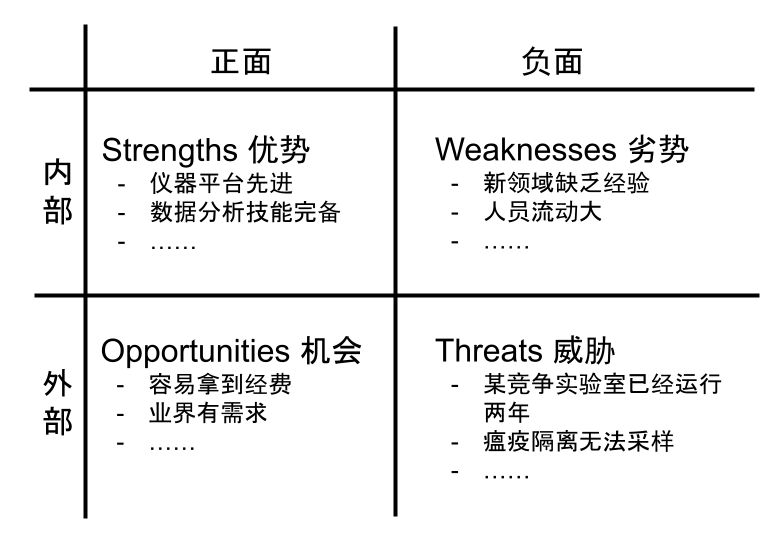
\includegraphics{data/SWOT} \caption[SWOT分析法演示(这里演示的是一个新课题组长的分析过程,列举优势劣势机会威胁后下一步要对其进行排列组合思考对策)]{SWOT分析法演示(这里演示的是一个新课题组长的分析过程,列举优势劣势机会威胁后下一步要对其进行排列组合思考对策)}\label{fig:unnamed-chunk-41}
\end{figure}

每一个项目事先要进行规划。项目规划期间要发挥团队作用,进行内部头脑风暴,每个人都提出跟主题相关的内容,做成思维导图。然后对事项按工作量与影响力进行区分,选取工作量低但影响力大的方案。计划的目的是了解情况而不是制定教条,要预留结果不理想后的其他方案或灵活度。然后分拆出具体有时间期限的可执行的步骤,时间安排上可根据\href{https://wiki.mbalib.com/wiki/\%E6\%97\%B6\%E9\%97\%B4\%E2\%80\%9C\%E5\%9B\%9B\%E8\%B1\%A1\%E9\%99\%90\%E2\%80\%9D\%E6\%B3\%95}{紧急重要四象限}来设计,优化步骤让所有事都在重要但不紧急的阶段完成。然后对项目的安全与经济风险进行列表,设计紧急预案,做到执行成本可控。这个方法又称作艾森豪威尔法则,因为艾森豪威尔说过:我手中的待办事项可分为两个种类,``紧急''和``重要'',重要的事情永远不会紧急,紧急的事情不会重要。

\begin{figure}
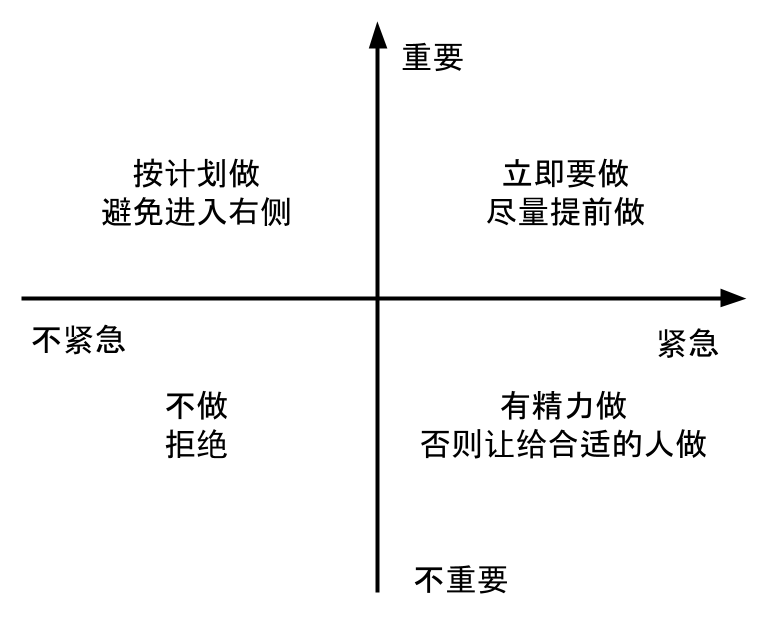
\includegraphics{data/Eisenhower} \caption[紧急-重要四象限及其对策]{紧急-重要四象限及其对策}\label{fig:unnamed-chunk-42}
\end{figure}

实际科研并不是围绕单一项目,每个个体会有自己主导的课题,也会参与其他人的项目或同时主导多个课题。此时要做好整体时间安排,利用不同研究项目切换来转移压力放松,保证时间都浪费在有意义的事上,这里可以使用\href{https://zh.wikipedia.org/wiki/\%E7\%94\%98\%E7\%89\%B9\%E5\%9B\%BE}{甘特图}来做时间规划。以项目为中心的管理是不同于被安排分工的传统模式的,需要扁平化管理,每个项目立项后有独立责任人与分工,项目完成则解散项目组。团队超过10人就要分拆,项目由需求与进展来指定或轮转个体角色,更好锻炼团队每个成员的综合能力,也避免个体螺丝钉化。

项目执行中最大问题是拖延症,此时可参照计划中分拆出具体可执行的步骤来按部就班,执行时不思考整体,关注当下并进行记录,分阶段有始有终,每一阶段要停一下或定期整理记录并思考过程中出得问题与解决方案。如果对后续执行作出修改,一定知会所有团队相关成员。拖延症本质上是跟未来的自己博弈,如果自己对自控力没信心,可以尝试软件开发中的\href{https://www.allthingsdistributed.com/2006/11/working_backwards.html}{向后工作法} :先公开新闻稿,写问答,写用户文档,最后去写代码。在向后工作法中,你会受到来自外界的监督压力,也会在项目开始阶段就考虑审稿人或同行的批评,这样执行时目的更明确。项目进行中遇到新知识或者请教懂得人,或者自学,不要不停犹豫不前,随时把执行放在第一位。如果需要自学,推荐- \href{https://zh.wikipedia.org/wiki/\%E5\%BA\%B7\%E5\%A5\%88\%E5\%B0\%94\%E7\%AC\%94\%E8\%AE\%B0\%E6\%B3\%95}{康奈尔笔记法}与费曼学习法。前者强调回顾,后者强调通过教或写文章总结来学,一般人对新知识自己理解要求低于对他人输出知识的要求,当你需要教别人或公开自己的学习笔记时,会更严谨对待,也是跟自己惰性的博弈。

项目完成后要对项目进行回顾并整理成报告存档。项目计划就是项目报告的前身与扩展,做好文档的版本管理即可。项目计划的步骤与实际步骤没必要一一对应但要有记录,报告要附带对原始记录的索引或直接将原始记录贴上去,所有针对项目的讨论与进展都要体现在报告里。报告可以同时附带更新幻灯片版,在拿到数据的同时做出发表质量的图像,如果需要对外报告可以在半小时内拿出成品。最终报告除了结果也要总结过程得失,特别是对比实际过程与计划步骤的差距,进而优化下一个项目的计划。

这是项目报告模版:

\begin{itemize}
\tightlist
\item
  题目/开题时间/项目参与人
\item
  研究目的
\item
  SWOT分析
\item
  团队头脑风暴脑图与预案分析
\item
  可执行步骤的时间规划
\item
  风险预案
\item
  实际步骤记录与分阶段总结
\item
  结果与讨论
\item
  结论
\item
  得失与下一步计划
\item
  附录
\end{itemize}

\hypertarget{ux7ecfux8d39ux7ba1ux7406}{%
\subsection{经费管理}\label{ux7ecfux8d39ux7ba1ux7406}}

课题组运转需要经费,经费来源主要是分为纵向课题与横向课题。纵向课题经费一般指来自国家财政拨款的经费,如果课题组依赖平台,经费可能是直接划拨,否则是由课题组成员以个人或合作者名义向国家自然科学基金委、教育部、科技部等国家级单位或省市级单位申请获批的。横向课题经费则是课题组通过依托单位或自己从政府以外的机构获得的资金,可能来自企业,也可能来自于非盈利机构。按经费性质可以分为支持个人的与支持项目的,前者使用比较灵活,经常与奖项荣誉挂钩,后者则专款专用,事实上支持个人的经费通常也会限制在科研用途。

对于个人而言,成立课题组时所在单位应配置一定启动资金用来开展科研工作。之后可以阶梯申请国自然、面上、重大项目等以项目为中心的基金,也可以走个人属性比较重的青千、优青、杰青、长江学者等的申请。个人可以作为项目负责人,也可以仅仅就是以合作形式来获取运行经费。要合理根据申请限制来规划申请进度,防止出现经费断档的尴尬。

课题组应根据规模要研究需求来使用人力资源。课题组规模在十人以下时,大概会有一多半不同年级的硕士博士研究生外加一到两名博后与一到两名研究助理或实验室管理员,每年完成成果不少于三项,此时课题组长可借助院系实验室平台来管理课题组行政事物。当课题组规模超过十人,应配专门科研助理或进行课题组分拆,应尽量保持管理扁平化规避层级管理中信息交流不畅的问题。此外课题组可能要负担组内成员的工资,理工科运行经费要在百万人民币量级,而经费中大概两成可以用来作为工资或劳务费且都需要按预算执行,另外院系平台也会按比例向获批经费收取管理费来运行辅助科研的行政、后勤等支撑部门,实验室与办公室也会收取租金与水电费。

基金申请不可使用已经完成的结果,但可提供部分预实验结果来进行支持。要提供摘要、参与者、预算信息,重点给出立项依据、研究内容及关键科学问题、可行性分析,要提供项目特色与创新点并给出时间表。此外,基金申请通常也需要提供研究基础与工作条件方便评审者评估。

基金申请一定要事先看好关键时间节点与年龄节点,评审结果通常有评分,评分超过一定标准才能进入进一步筛选,认真阅读评审意见但没必要完全迎合评审人兴趣。项目获批后一般都需要中期进度报告与结题报告。所有报告都要存档并能追踪到撰写者与原始\href{http://journals.plos.org/plosbiology/article?id=10.1371/journal.pbio.1002333}{数据}。另外基金申请如果要求在发表论文中注明,请仔细核对申请号。

\hypertarget{ux5fc3ux7406ux8f85ux5bfc}{%
\subsection{心理辅导}\label{ux5fc3ux7406ux8f85ux5bfc}}

课题组长或研究生导师应重视自己与研究生的心理辅导,学校与机构应提供免费或补贴的心理咨询。研究工作极大概率会遭遇不顺,伴随的心理压力会很大,负面情绪要学会自我及时疏导与排解,不要排斥寻求外部帮助。

对于课题组长或研究生导师,外部压力来源主要是课题组运行经费筹集与学术荣誉评比。课题组规模要提前根据经费规划,不要盲目扩张或收缩。学术荣誉其实是别人说了算,重在参与,是非功过让时间来说话。研究上的不顺利可以通过教学来互补,正确评估自己的实力,可以激流勇进,也学会激流勇退,为后来者铺路。同时,当研究生目的不在科研时,可以沟通协商后制定退出策略,不要把自己的压力过多转嫁给学生。当学生比较脆弱无法承受项目失败时,要及时中止或暂停项目,预防极端现象。

对于研究生,在读期间会有来自家庭、男女朋友、导师、同龄人的各种压力。因为时代在变,导师、父母还有亲友不一定能理解你,同龄人能理解但可能不但没有解决方案反而给你更多压力。不过,请理解导师与父母会经历你也无法理解的他们成长年代的艰辛,他们看你们总会觉得你们条件比他们好很多,这些都是正常的,人与人间互相理解是小概率事件,所以我们才通过制度与标准降低理解门槛,但这些很难照顾到当时感受。当你被压力折磨时,可以通过发展个人兴趣爱好来转移注意力,但真正能消解压力的还是对未来的信心。读研走科研这条路对于一大半的人而言是死胡同,现有资源无法保证舒舒服服做科研但不用承担失败责任,因此肄业或拿到学位转行是常态,及时跟导师或更高层管理者沟通。要理解导师不见得是心理健康的人,沟通无效可选择转导师。

总之,没有人是天生的抗压者,也不存在零风险的科研,及时的心理辅导对于导师与研究生都很重要。在制度平台不够完美时,请构建不影响别人与伤害自己的自我疏导方式。

\hypertarget{ux8bb2ux8bfe}{%
\section{讲课}\label{ux8bb2ux8bfe}}

现代科研人员所在的研究机构通常会承担教学任务,本节会重点讨论讲课相关的注意事项。

\hypertarget{ux5b66ux751fux5982ux4f55ux5b66ux4e60}{%
\subsection{学生如何学习?}\label{ux5b66ux751fux5982ux4f55ux5b66ux4e60}}

首先搞清楚你自己学科里学习的含义,如何去掌握知识,自己在学习过程中有益的经验。学生的学习方法有深入学习、策略学习还有表面学习。了解个体学习的差异如何影响学习效果,例如前置知识、动机、学习策略还有对于学习智力能力的信仰。掌握元认知方法,掌控自己的思考过程。明白教学是承前启后的受多方面影响,要根据内容与学生调节教学方法,要知道学生对不同教学环境的应对策略。

\hypertarget{ux5982ux4f55ux6fc0ux52b1ux5b66ux751f}{%
\subsection{如何激励学生?}\label{ux5982ux4f55ux6fc0ux52b1ux5b66ux751f}}

激励就是让学生渴望或乐意做某事。激励的理论模型:

\begin{itemize}
\tightlist
\item
  期望-价值理论:学生对目标有一个期望并对这个期望有一个价值判断
\item
  成就目标导向理论:有些人是掌握目标导向,有些是表现目标导向
\item
  成长-固定思维模式:有些人认为能力可以不断发展,有些则认为无法变化
\item
  自我表现理论:人类三个基本需求:能力认可、归属感及自治
  激励方法就是让学生提高激励的体验,例如预先教一些技术提高完成度、课前测试、让学生选择主题、分享学习经验、提供正面反馈、考核时比较灵活(6次作业取5次成绩)
\end{itemize}

在教学时要考虑作业与评价方式、学习活动、反馈还有课堂气氛。给予学生主动权,提高存在感与社交活跃度,建立对教学行为评价的持续反馈机制,记住学生的名字\ldots{}

\hypertarget{ux8bc4ux4ef7ux5b66ux4e60}{%
\subsection{评价学习}\label{ux8bc4ux4ef7ux5b66ux4e60}}

学习金字塔从下往上:记忆-理解-应用-分析-评价-创造,可参照设计不同难度的考核。学生学什么与怎么学经常依赖于如何被评价,评价有三种形式:

\begin{itemize}
\tightlist
\item
  诊断式:小测试、涂鸦板、头脑风暴、一对一会议、思维导图还有概念测试
\item
  形成性:让学生提出最难懂的问题、一分钟论文、小抄、随堂测试(给出比例)、同行评议、反馈、问题集、非正式展示、进展报告
\item
  总结性:期中期末最终展示
\end{itemize}

教学目标、教学行为与反馈之间要相互有联系,给出指引,自己先完成并且对学生作业做出点评。

\hypertarget{ux8bfeux7a0bux8bbeux8ba1}{%
\subsection{课程设计}\label{ux8bfeux7a0bux8bbeux8ba1}}

从教学目标、教学形式和评价三个方面入手考虑课程设计。首先整理课程概念,头脑风暴选出来以后思考概念间的联系,反复思考概念间的相互关系。课程结束后可以让学生自己去绘制自己的课程地图。教学目标上从学生角度出发,考虑他们通过课程知道什么、做什么以及有什么样的感受,就是从脑、心、手三个方面去设立,用强动词例如解决、设计、定义、评价而不要用知道、理解等词来设立目标。评价方法参考上面评价章节。教学形式上明确学习时间不同于上课时间,提供知识与实践反馈,采取主动教学等策略,可参考布鲁姆分类学,另外教案与视频要做到在线化。

\hypertarget{ux4e92ux52a8ux5b66ux4e60}{%
\subsection{互动学习}\label{ux4e92ux52a8ux5b66ux4e60}}

互动学习是提高课堂参与度的组织形式,例如分组相互讨论。课程设计可以按照预热-小教程-团体活动-分享来划分时间。翻转课堂也可以作为一种互动学习的手段来尝试。

\hypertarget{ux6559ux5b66ux7406ux5ff5}{%
\subsection{教学理念}\label{ux6559ux5b66ux7406ux5ff5}}

教学理念是教学档案的一部分,常用来作为简历教学经历的补充。一般一页,列举三个教学理念。整理教学理念常用来整理自己关于教学的理解,作为教学的行动指南,也可以用到教育相关工作申请上。首先去思考理念的来源与如何起源,然后可以采用隐喻来阐述教育理念,例如园丁、教练、瑞士军刀等。

这里简单介绍下常见的教学理念:从已知到未知,也就是在教授任何新东西前先要介绍原来就有或者之前教过的概念,然后从已知概念存在的问题入手,揭示新概念的必要性,打个比方,想讲解持久性有机污染物这个概念可以先从DDT农药这一相对简单的概念开始讲,然后过渡到存在类似问题的其他污染物,最后自然引导出持久性有机污染物的概念;费曼学习法,就是鼓励学生以教代学,把自己刚学会的东西教给另一个同学,当另一个同学提出问题时去反思自己的理解哪里有问题,然后不断加深理解,相当于通过反馈来提高理解力;与费曼学习法类似的一种教学理念是苏格拉底式提问,通过不断的向学生质疑促进学生的思辨能力,当然这个方法用得好学生受益匪浅,用不好杀人诛心。

\hypertarget{career}{%
\chapter{就业}\label{career}}

在第三章中我们提到了博士存在的就业问题,就结果而言,博士在博士阶段结束后选择博士后更多是为了下一人生阶段的就业制造机会,而就业不仅仅只是学术界。本章将重点讨论就业相关议题。求职过程一般包括投简历、搭人脉、面试、获得职位、事业发展等流程。这里还是要强调,伴随扩招与产业升级,取得博士学位后最终留在学术界的比例会越来越低,本章所讨论的问题哪怕你目前认为用不上也最好了解下。

\hypertarget{ux5546ux4e1aux4e0eux5b66ux672f}{%
\section{商业与学术}\label{ux5546ux4e1aux4e0eux5b66ux672f}}

商业的两条规则:营利与持续改进,所有的招聘信息会根据这两条规则来设计。学术界与之对应的则是成果发表与持续改进。其实商业与学术界都有周期性,在学术界,你的周期是:

\begin{itemize}
\tightlist
\item
  提出假设
\item
  成立研究团队
\item
  设计实验做实验
\item
  成果投稿与发表
\item
  改进或提出下一个假设
\end{itemize}

而商业周期则是:

\begin{itemize}
\tightlist
\item
  提出目标
\item
  成立项目组
\item
  执行与生产
\item
  市场检验与宣传
\item
  调整或提出下一个目标
\end{itemize}

你会发现这两个并不矛盾,技能要求也类似,你所需要的是把学术用语转为商业用语。而商业所需要的技能集主要包括创新与风险管理、生产力改进、执行控制与财务规划。

同时有些技能在学术界与商界是通用的,那就是团队管理与交流等社交技能。当你具备这些技能后,进行职业转换其实就是换一套术语体系讲故事。有些主题例如项目管理与时间管理等内容前面章节已经叙述可自行对应。

\hypertarget{ux7b80ux5386}{%
\section{简历}\label{ux7b80ux5386}}

就业的第一步永远是了解自己,尽早进行自己的个人发展规划(individual development plan,IDP)。所谓个人发展规划,就是要对自己的技能、兴趣还有价值观进行评估。所谓技能,就是你能为别人或企业提供的能力,这是招聘方视角重点关注的,要学会从别人视角给自己的能力列清单。兴趣就是你想做的事或理想的事业,这个可能与你的技能匹配或不匹配,但无论如何你得知道自己想要什么。所谓价值观,就是你工作会看重的东西,薪水、团队、安全感等都算。个人发展规划的目标就是把技能、兴趣与价值观列出来然后下阶段努力把这些对齐或调谐,以此为找工作的指导方向。只要你肯列出来,就会消除很多迷茫,有些岗位也许光鲜但不对你胃口,有些岗位短期内痛苦但可能最大限度实现你人生价值,此时有这样一个规划一对比就清楚很多了。网上也存在大量量化的个人职业测评之类的产品,但本质就是要在找工作前充分理解自己对别人的价值及自己想要的价值。

投简历要搞清楚cv跟resume这两个概念,cv 是完整的个人信息,resume一般1-2页,结果导向或者是根据不同职位打造不同 resume 而不是一个文本走天下。招聘中一般只用resume而cv一般是存档或背景检查用的。resume会包含个人陈述部分而cv更多是事实罗列,个人陈述部分一定是要与招聘信息有呼应,符合的条件要多说但不具备的别瞎说。你需要日常维护cv,求职时则要根据招聘信息对cv进行优化。一份简历至少要包括个人联系信息、教育经历、工作经历与成果。有两点要注意:对外对内要用不同邮箱进行区分且最好有个人简短不重复的ID,这对招聘方来说比较有利。

一条招聘信息通常包含三层技能需求:科研技能要求、商业技能要求与社交技能要求。毕业生通常只会关注科研技能要求但其实科研技能要求虽然是门槛,但造成职业竞争力差异的并不是科研技能,而是商业技能与社交要求是否在简历中体现,特别是那些在招聘信息里写的很清楚的却常被忽视的。一份招聘如果标注了团队能力、项目管理就要针对性对你自己的经历进行描述。这些三层内容要在简历的个人陈述中分段体现,给招聘者的信号就是你不但读了招聘信息还读懂了企业的需求。

与简历相关的是求职信(cover letter),通常来说如果没有特别说你要提交就可以告诉招聘者简历是不是目的性的及覆盖的内容,然后就是留下联系方式,简明扼要不要重复简历内容。如果你有与招聘者的社交联系或正面评论等简历里不合适出现的内容可以在求职信里提,例如读过论文及会议上留意过展台,一定要诚实,很多东西大家都懂但不同的表述方式会产生不同效果,这也是你对外交流能力的体现。在邮件联系时要礼貌(及时发送感谢信)且及时跟进(follow up),正常人都想做个好人,特别是对弱联系或一面之缘的人。

\hypertarget{ux4ebaux8109}{%
\section{人脉}\label{ux4ebaux8109}}

简历的准备主要不是指望海投可以投中,而是在理想职位出现后通过最合适的人替你内推并拿到面试机会(占比80\%)。不论职场还是学术界,人们都喜欢从了解的人那里获得推荐候选人,一方面有人背书,另一方面海投过来的信息存在大量非目的性简历而筛选简历经常是很任性的过程。你的求职目标就是找一个自己喜欢且招聘方也会对你满意的职位,不了解自己与对方需求的简历是对双方时间精力的浪费。

在于陌生人建立联系时,可通过亲朋好友或校友老乡等入手,也可以参与主题聚会并通过共同场景建立联系。不同于学术界,社会职场每个人的知识背景是不一样的,不要使用专业术语来跟非专业人士交流。一个合格博士需要有能力用通俗语言跟他人交流,特别是你的研究内容,全是专业术语更多显示的是对本质的不理解。事物可以是复杂的,但不能是说不清楚的。

在与人交流时一定要意识到每个人都是独立的个体,有自己的性格与处事方式,即使跟你不一样也不代表就更厉害或不好。这种对他人的理解首先要建立在对自己的理解上,在你眼里也许自己很完美,但在别人眼里可能存在不同解读,你可以不在乎但不能不知道这种可能性的存在。同样,对别人也不要轻易评价与人云亦云,要能体会尊重他人的独特性或制定相应高效交流方式。你建立联系的人要提供其建立联系后额外的价值或引起兴趣,如果一味放低姿态,对方可能不会尊重你。

商业培训里喜欢用MTBI测试来对职场中人格进行分类。你可以先做一套测试,然后你会得到四个字母来描述你。每个字母代表一种二分法,例如I代表内向而E代表外向,N代表直觉而S代表感觉,T代表思考而F代表情感,J代表判断而P代表感知。虽然学界对这个没有统一意见但不妨碍很多人在用这个对人进行预判与交流方式的试探,例如对于一个TJ的人随意改变计划几乎是不可接受的。

职场人对外交流有三个标签:机构、职业与个人。陌生人间的交流最好从个人经历出发而不是社会机构角色出发,后者是机械且标签化的,不利于有效沟通。对外交流要了解镜像神经元理论,也就是交流双方都会在交流中不自觉尝试模拟对方促进交流,而镜像神经元更多依赖行为与语言引导。一个常见的技巧就是专家到学习者的角色转换,当别人问你问题时,不要着急堆砌专业词汇,而可以反问对方问题来切换为学习者角色来更多了解事实并最终提供其原始问题的答案。

具体训练交际技能可参考3M\&M方法。当A问B一个问题时,B反问A三个问题,问问题前吃一颗糖豆来给自己思考时间而不是用本能去情绪化回答问题,得到答案后再回答A最初问题,提问过程中要注意对方性格类型与情感诉求,然后用个人角色出发在理解同情角度解决或回答对方提出的问题。另一种练习的方式就是准备电梯报告,请参考前一章相关内容。

在建立了有效的联系后,你需要一定的维护,可以通过邮件往来或社交网络关注。注意,你不需要很密切的联系而是更多让对方对你有一个角色标签,这样对方遇到合适职位时会联想到你。而另一种联系方式就是信息面试( information interview),当你特别想取得一个职位时,需要通过人脉来非正式了解情况,此时可以约下相关人来聊天。首先你要自己进行一定调研,这样不浪费双方时间,然后准备好帮助对方想起你的自我介绍,然后对话以寻求建议与背景信息为主而非针对职位,可以涉及对方的背景、日常工作及其建议,特别是在招聘信息或官方网站上没有提及的内容,对话后发送邮件表示感谢。

\hypertarget{ux9762ux8bd5}{%
\section{面试}\label{ux9762ux8bd5}}

要做好充分准备,了解公司运营、财报、新闻,从社交网络里获取面试人的角色信息。要尊重面试官,眼神要直视,回答问题前要停顿一下过脑子,多听少说别打岔。回答问题可采用 STAR 方法,也就是场景(situation)- 任务(task)- 行动(action)- 结果(result)。先给出场景,然后描述你的任务,然后叙述你采取的行动并最终总结结果,要言之有物。

下面是常见的面试问题,可事先准备或练习:

\begin{itemize}
\tightlist
\item
  介绍下自己
\item
  你的哪些科研技能符合职位要求
\item
  你跟其他候选人的最大区别是什么
\item
  举一个你提高实验室效率的例子
\item
  实验不成功如何处理
\item
  如何训练实验室新人
\item
  讲一个别人让你失望的例子
\item
  讲一下你用来保障你研究优势的策略
\item
  当研究中出现意外与挑战如何应对
\item
  描述下你当前研究的工作流程
\item
  你的研究专长是如何应对外部挑战的
\item
  你是如何帮助同事解决你专长的问题的
\item
  除了科研技能,你了解哪些商业技能,你是否应用过
\item
  描述一个外部机遇下你如何扬长避短
\item
  你如何利用人脉来为岗位提高生产力
\item
  讲一个实验室外体现你领导力的案例
\item
  你当前研究的商业价值是什么
\item
  给你1000万美金,你会投给谁
\item
  我们为什么要雇佣你
\item
  基于你的背景,我们能给出的薪水是XX,你会接受吗
\item
  你当前研究项目的成功标准是什么
\item
  你当前研究项目最贵的组成部分是什么
\item
  讲一个你管理时间的案例
\item
  你当前工作的里程碑是什么
\item
  你入职五年的职业计划是什么
\end{itemize}

从面试官角度,他们会重点关注回答的内容是否容易理解,是否完整且会记录时间,不同面试官打分的项目不同,他们会根据结果整体去考察候选人,直接拍板的招聘要警惕。

\hypertarget{ux804cux573a}{%
\section{职场}\label{ux804cux573a}}

日常工作中要懂得向上管理,也就是合理向你的上级表述你的需求、意愿来达成你的工作目标。向上管理意味着你的角色是主动的而不是被动的,对于工作推进总是积极态度而不是一味听指挥。与上级不同意见时,要用对事不对人的态度从数据、外部环境等客观事实出发解释不同决策下会出现的不同境遇,把决策权有导向性的给上级进行传递。同时,要对上级利益关系有清楚了解,如果上级阻碍你的长期个人发展,尽早考虑下一份工作而不是长期内耗。

给同事或上下级反馈要采取绩效反馈(performance feedback)的方式来进行持续改进与量化评价管理(例如six sigma 的黑带认证)。不要泛泛而谈大道理而是专注到具体的事,不要针对个人而是针对行为表现进行反馈,目标是为了帮助而不是打击,给出的意见要具备可执行性且点到为止,要在反馈中询问对方是否听明白,然后之后要跟进结果。在发现低效行为时马上进行反馈纠正,指出期望与评价标准,阐述行为后果与高效的行为后果并鼓励改进,不要抓着一点不妨且避免公开指责,设定截止日期来检查结果,向前推进。发现高效行为时要马上嘉奖给予正反馈,也要指出你的评价标准与该行为对目标的帮助,鼓励是为了保持高水平绩效。

职场里谈判分为分配式谈判(distributive negotiation)与整合式谈判(integrative negotiation),前者是零和博弈非此即彼的谈判而后者是提供双方额外价值的双赢谈判,尽量将谈判做成整合式的而不是分配式的。职业是会换或者需要晋升的,你个人在人生不同阶段需求不一样,对应的职业需求也不一样,一般三到五年一个周期进行调整,原则上非升即走。升可以包括福利升级、工资升级、岗位升级等。在加薪谈判中要更多用数据说话并站在提供更多价值角度择时择机进行整合式谈判。但安于现状或进行工作生活平衡也是个人选择自由,请根据自身需求提出要求。另外,要了解团队加入你或不加入你的区别,这样就知道你自己对外的价值。从公司角度,他们会压低每个人的重要性而保证整体价值最大,此时他们就会出现功能冗余,大公司几乎都会过度雇佣。在一个联盟里,要知道自己的夏普利值,也就是在不同加入次序下你对团队完成任务的平均贡献。在投票中,夏普利值并不与人数对应,团体代表如果达不到一定程度,可能存在就算人数不少,但决策能力为零的情况。

职场成功要牢记这个公式:

\[成功=a×实力+(1-a)×运气\]

搞清楚自己实力与运气的比例,如果你运气很好,那么某个职位上就要虚心多去请教前辈才能更上层楼而不是感觉无所谓。运气只有在实力相当时才会起作用(实力悖论),否则德不配位就比较麻烦。

职场也需要成长,很多公司意识到员工的成长可能带来更高的回报后会持续请人来进行培训。培训的内容可能是新的技术,也可能是新的理念,公司会为员工进修报销,有的连读学位的钱都能出了。如果你所在公司提供进修的福利,一定不要浪费,现代社会每个人的成长都是贯穿终生的。

职场中的项目管理与学术项目管理类似,参考前一章内容。

\hypertarget{ux804cux4e1a}{%
\section{职业}\label{ux804cux4e1a}}

下面列举一些博士的就业方向,仅供参考。

\hypertarget{ux535aux540e}{%
\subsection{博后}\label{ux535aux540e}}

欧洲有玛丽居里博后与洪堡学者,日本有学术振兴会(JSPS),美国国立卫生研究院有 T32 (美国毕业2年内的博士,30\%通过率)与 K99 博后(博士毕业4年内,23\%通过率)。博后要搞清楚经费来源是软钱(soft money)还是硬钱(hard money)。前者 是教授申请项目中用来支持博后的经费,一旦用光了位置就没了。后者是学校从学生学费或研究机构募集后分给课题组用来研究的经费,用光风险比较小。博后自己申到软钱可摆脱课题组对课题限制。企业博后则有较高收入且与业界结合紧密,但转回学术界会略有困难。此外,如果是,可以申请F32

博后是学术界犯错有人兜底的最后一站,如果不出结果可以选择退出学术界,毕竟现在的博士毕业人数根本不可能都在学术界内消化掉。说白了博后是就业前的临时身份,所有博后阶段都要围绕就业规划。如果把博后当成推迟接触社会的避风港保持象牙塔的生存状态,就业所需要的能力得不到提高,那么很难成为学术界的独立研究人员,更不用提转行跨界所需要的能力了。

\hypertarget{ux5e38ux4efbux8f68}{%
\subsection{常任轨}\label{ux5e38ux4efbux8f68}}

常任轨包括研究教授与文理学院教授,目前国内多采用非升即走与稳定事业编两套体系,对自己实力有信心就去选非升即走。在没拿到终身教职之前,常任轨教职可能被看作高阶版博后,因为相对独立,所以会有经费压力,但如果连独立课题组都没有,那么可直接认为就是博后加长版。这一阶段需要给自己在学术界内建立影响力,同时可能也要承担教学任务。拿到终身教职最大的压力就是经费,大量的时间要放在找合作关系与经费申请上,此时要兼顾研究者与课题组管理者身份。

\hypertarget{ux975eux5e38ux4efbux8f68}{%
\subsection{非常任轨}\label{ux975eux5e38ux4efbux8f68}}

研究性教职或偏行政工作,这样的岗位适合只看重老师身份的人去做,通常你的经费来源由课题组长或研究所来兜底。不过非常任轨的职位很难做到完全独立,经费与研究方向跟着项目走,不过相对压力也小。偏行政方面有一类属于科研项目经理,主要负责对接基金申请与技术转化的事。这类职位需要有一定科研背景或学历要求但不需要你去做科研。

对于研究机构而言,常任轨教职是精英化的,很难维持一个很大的体量。现在越来越多的机构设立非常任轨教职来吸纳高学历研究人员做项目或辅助,很多职位其实是给过了年龄的博后准备的,因为确实存在很多研究人员既不想转行也无法长期保持博后身份做想做的研究。伴随学历通胀,这类职位可能在未来变得更普遍。

\hypertarget{ux975eux9ad8ux7b49ux6559ux80b2}{%
\subsection{非高等教育}\label{ux975eux9ad8ux7b49ux6559ux80b2}}

k12教育,教育研究为主,更多人选这个是为了下一代。给小学中学生当老师是很多博士的最终选择,在他们看来降维就业是平衡工作生活的最佳选择。不得不承认的是k12教育在现代社会里确实属于高投入高产出的行业,家长对这一阶段孩子的成绩期望也确实能从高投入里看到成果,对于学校而言就意味着招募高学历教师。相比之下,研究工作则会遇到高投入零产出的问题。因此,k12教育中高学历从业者可以拿到稳定的收入与较高的社会地位,然后把自己的应试技巧传承下去。想从事这个行业,最好去拿个教育硕士或者提早去考教师资格证,否则后面事业发展受限制。

\hypertarget{ux79d1ux5b66ux987eux95ee}{%
\subsection{科学顾问}\label{ux79d1ux5b66ux987eux95ee}}

律所、金融行业需要,注意细节拼写与写作,国内虽不常见但会越来越重要,也是科研人员转金融法律专业人士的重要途径。其中,最常见的高学历科学顾问一般是帮忙来审核专利的,要通过专利方面的考试。金融律所行业之所以雇佣科学顾问,一定是他们带来的收益远高于付给他们的工资。很多科学顾问在很多收购并购案、团体诉讼还有知识产权纠纷中会起到特别关键的作用,如果你的竞争对手或诉讼对手没有科学顾问,那么相同的证据摆出来解读的结果可能完全不同,这也是从事科学顾问行业的人很多最后都做到了合伙人级别的职位的原因。在律所与金融行业里,知识不仅仅是力量,还可以转化为财富。

\hypertarget{ux79d1ux5b66ux4f20ux64ad}{%
\subsection{科学传播}\label{ux79d1ux5b66ux4f20ux64ad}}

把自己的成果讲给别人或把别人的成果通俗讲给大众,需要写作技巧的专门训练。需要的知识大部分内容与前一章类似,不同的在于要针对不同媒体掌握不同交流方式,例如视频跟音频的展示策略,自己演讲还是一问一答等。要始终遵守从已知到未知、从结果到原因、从简单到复杂的讨论模式,否则观众或读者会跟不上你的思路或失去兴趣。公众喜欢听故事但很多科学问题可能有头无尾,此时也要会一些开放式结局的结体手法。学会用网络流行语、形象化语言与多媒体方式来跟无背景知识的人交流但要保持严谨,千万不要堆砌专业术语,这样不但不利于科学传播,反而会加剧科学宗教化的印象。

另外科学传播会更侧重对读者需求与认知水平的尊重,不能动不动就说某某是众所周知的。受众越广,就一定会出现嫌弃讲的过于简单或专业的评论,你只需要为大多数观众或读者负责就可以了。一定要事先了解观众或读者的基本情况,然后去调整内容,可以在报告开始阶段做二维码调查来引起观众兴趣并掌握一些基本情况。提问阶段有人偷换概念过度延伸也是正常的,此时要学会聚焦主题。另外最好事先准备一些常见问题的答案放到报告小册子里防止时间不够用。要学会时刻表示友好而不是跟审稿人一样刻薄,读者或观众带着兴趣来最好带着知识而不是负面情绪走,这就完全不利于科学传播了。

现在国内常见的科学传播职业基本都在自媒体,有些是学术机构的科学传播部门建立的,也有传统媒体转行过来的。只要内容足够优质且对写作有兴趣,借助互联网订阅、线下活动、图书出版等方式都能获得不错的薪资。

\hypertarget{ux653fux5e9cux516cux52a1ux5458}{%
\subsection{政府公务员}\label{ux653fux5e9cux516cux52a1ux5458}}

选调生或定向培养是研究生及以上从政人员的职业途径,但走得高就要放的深,从基层才能累积最务实的经验。博士从政现在不算新闻了,学者型官员目前也比较流行,当然这说的是两回事。博士从政指的是博士毕业就去地方任职这类,一般得是名校选调生才行。博士从政属于典型起点高经验少的公务员,如果没有政绩,很可能就业即巅峰。学者型官员是指在研究机构内走行政路线,一般得到学院院长或副校长这个级别才有可能被调入政府行政部门做官。学者型官员通常需要有政府机关借调或者社会兼职的经历,如果学术水平也不错,那么可能一步就从学术机构管理层转到国家部委等实权单位任职,或者通过智库顾问的方式参与政策制定。想做好公务员,一定要有足够的基层经验、很强的办事能力及社交能力。一路读到博士然后跑去从政的人志向都不可小觑。

\hypertarget{ux975eux8425ux5229ux7ec4ux7ec7ux4e0eux57faux91d1ux4f1a}{%
\subsection{非营利组织与基金会}\label{ux975eux8425ux5229ux7ec4ux7ec7ux4e0eux57faux91d1ux4f1a}}

很多博士就业最终会选择非营利组织或一些私人慈善基金来工作,薪酬上可能会比较低。选这类工作一般是打算追求个人理想的,但这些机构的运行却不是理想化而是现代化的。非营利组织也会有研究机构、需要人来管理基金、协调学术界与业界。很多你在高校或研究机构能见到的职位在非营利组织与基金会里也有。从事这类行业,有热情是起点,关键还是领导组织能力与筹款能力,是人际关系的缝合怪。

很多非营利组织有智库的职能,经常会公布一些报告,资金来源可能是民间筹集或政府。国内智库多多少少有点政府背景,很多是从原来政府机关的政策研究室一类的地方剥离出来的,另外一些则直接可以看成研究所或大学附属机构。智库有时候也是学者转官员或者商人转官员的一个身份过度机构。不过博士就业进入智库的相对比较少,智库对于经验的要求多过对学位的要求而且薪资一般。如果你打算搞清楚政策是怎么制定的,那么可以去智库体验一下,否则可以等你有想法转换职业的时候再考虑不迟。

\hypertarget{ux7f16ux8f91ux51faux7248ux793e}{%
\subsection{编辑/出版社}\label{ux7f16ux8f91ux51faux7248ux793e}}

认真严谨但更重要的是对学科前沿的把握,目前学术期刊倾向于雇佣职业编辑处理稿件及推广,所以要懂点现代社交网络及传播学。当前伴随开放获取的流行与大出版集团对优质稿件的竞争,很多的期刊编辑逐渐从学术兼职的专家教授转为专职人员。专职编辑人员一般都有博士学位或博士后工作经历但并不要求很高的学术水平,出版集团雇佣专职编辑主要是为了加快稿件处理速度并且应对科研领域的一些新生事物,例如预印本还有自媒体等,这些编辑通常会比较年轻且乐于接受新概念。供职于出版集团或学术期刊的专职编辑工作时间、地点都比较自由,大部分工作都可以通过互联网完成。此外,专职编辑是需要给出版集团带来利润或影响力的,很多出版集团看到了文稿润色、内部期刊转投、封面设计等业务的利润与影响力,专职编辑可根据具体情况推荐内部业务来服务读者与作者。

\hypertarget{ux5e94ux7528ux4e13ux5bb6ux53caux9500ux552e}{%
\subsection{应用专家及销售}\label{ux5e94ux7528ux4e13ux5bb6ux53caux9500ux552e}}

主要在科研仪器公司工作,为科研需求提供支持。这类工作一般是从应用工程师开始做,累积足够经验后转销售卖产品。应用工程师的工资是稳定的但相比销售低不少,销售主要收入是订单的提成,因为科研用仪器通常几十上百万,所以经常一年下来就需要跑几个大订单就能完成全年绩效。很多做应用转销售是看重了工作时间灵活自由,收入凭本事赚的特性。但不论应用专家还是销售,每年都需要经常出差,要么是拜访客户,要么是参与企业赞助的学术会议。想从事这个行业,最主要是保持跟之前实验室成员的联系,他们都属于潜在客户。如果做耗材,很多时候吃定几个实验室就能稳定养活一个小公司。

\hypertarget{ux4f01ux4e1aux79d1ux7814ux836fux4f01}{%
\subsection{企业科研/药企}\label{ux4f01ux4e1aux79d1ux7814ux836fux4f01}}

主要在药企与医学院,从事新药研发或实验,最重要是熟悉标准化流程,熟悉质量控制与质量保证。如果你能事先去搞一个六西格玛的黑带认证,那么你的工资会直接提升一个档次,也有可能被当成未来的管理者培养。新兴生物科技公司也会招收高学历的人做包含研发在内的各类工作。在公司做研发,团队成员的知识背景一般差异很大,以产品为导向来进行研究。如果你期望一个相对高的收入、相对宽松的研究环境与几乎为零的经费压力,那么这类行业值得尝试。企业科研的风险在于当外界经济条件非常差的时候有可能整个研发部门都被裁掉。

\hypertarget{ux533bux836fux4ea4ux6d41}{%
\subsection{医药交流}\label{ux533bux836fux4ea4ux6d41}}

这类职业有一定专业要求,需要生命科学或医学药学高学历背景。医药交流主要包括把科研进展带给医生的医学联络官(medical science liaison)
或帮助药厂把新药与疗法传播给客户(medical communication),收取佣金或抽成,要有强大的信息收集处理能力。这个行业是连接药厂、临床大夫与公众的中介,医学联络官薪资不比医生差但需要的技能更侧重交流能力,后面可能成长为医学顾问。

\hypertarget{ux54a8ux8be2}{%
\subsection{咨询}\label{ux54a8ux8be2}}

提供解决问题的方案,典型服务业,得有很强的甲方乙方感。咨询行业是少数只看学历不问研究方向的行业,想从事这个行业,必须要有名校学历撑门面,几大咨询公司的学历要求都非常高。此外,咨询公司招人很多也是走校友途径的,他们需要维护一个精英形象。想进这类公司,要有实习经历、要做模拟案例、要会画饼。不过,很多公司请咨询公司并不一定是他们遇到了无法解决的问题,而是他们需要一个光鲜亮丽的第三方经过层层研究用各种花哨新颖的概念名词给出一个他们内部不太好推进的改革方案。你要真是怀着解决实际问题的心态去做项目,那说明你还不了解甲方这个拥有五颜六色的黑心的现代社会物种。

\hypertarget{ux91d1ux878d}{%
\subsection{金融}\label{ux91d1ux878d}}

工作压力大但收入高,资金流全流程了解,需要洞悉名利场潜规则,容易过度职业化迷失自己。金融行业分为买方与卖方,刚入行一般都是卖方的银行、投行或券商,其主要任务就是将别人的资产包装后卖给买方赚取中介费或佣金,有的则是撰写行业报告或做咨询;买方则是手里有公募或私募来的大笔资金去寻找好的投资标的,赚的是管理费或收益提成。金融行业买方比卖方地位高的同时买方需要的团队也比卖方小,毕竟买或不买是决策,不需要太多人决策。大多数金融行业的人都想从卖方变买方,有科研背景算是一种买方加分。

\hypertarget{ux6570ux636eux79d1ux5b66ux5bb6}{%
\subsection{数据科学家}\label{ux6570ux636eux79d1ux5b66ux5bb6}}

分析数据,更多时候是洗数据与设计数据处理自动化流程,不需要自己写算法但一定要洞悉实际问题的背景知识。这里要说明的是数据科学家跟计算机科学家不一样,喜欢招不限专业博士的是数据科学家,计算机行业招聘几乎一定是限制专业的,所以你要是想做码农,一定要转行拿那边的学位,否则即使进入计算机行业你的博士经历也没有太大用。

数据科学家要同时具备专业知识、统计学知识与计算机编程能力,更多的时候要会传达需求给更专业的人士。数据科学家在不同行业做的事差异挺大的,有的侧重可视化、有的侧重数据库、有的侧重模型等,其实很多数据科学家的职位都有前身,换个名字有时候是为了适应时代需要。博士毕业做数据科学家是需要一些自学能力与相关项目经验的,这些恰好也是很多博士项目培养需要的能力,但并不是说所有拿到学位的博士都适合去做数据科学家,至少你的研究经历得涉及统计跟编程才能靠点谱。

\hypertarget{ux521bux4e1a}{%
\subsection{创业}\label{ux521bux4e1a}}

适合经济背景、技术独占性还有人脉三者兼备的人去做,不要妄想用一个强势因素去覆盖另外的弱势因素,要找靠谱的合伙人。现在创业有成绩的人并不是突发奇想蹦出来的,这些人大多在校园里就开始参加各类创业大赛累积人脉与技术资源,产品原型与中试可能都做过了。如果你博士毕业仅具备技术实力而没有创业经验,那么前面的坑实在太多。不过,高校一般会有一些专门的机构来辅导学生创业,有些甚至会帮助融资或用学校经费融资换股份。如果你打算创业,一定要充分利用学校给的试错资源,一旦走向社会,即便创业者有心当赌徒搏一把遇到的也大都是不同段位的骗子,能无风险骗到钱或技术他们绝对不赌。

\hypertarget{appendix}{%
\chapter*{附录}\label{appendix}}
\addcontentsline{toc}{chapter}{附录}

\hypertarget{ux73b0ux4ee3ux79d1ux7814ux5175ux5203ux8c31}{%
\section*{现代科研兵刃谱}\label{ux73b0ux4ee3ux79d1ux7814ux5175ux5203ux8c31}}
\addcontentsline{toc}{section}{现代科研兵刃谱}

工欲善其事,必先利其器。今天绝大多数知识都是工具生产出来的,也就是想使用知识,肯定要先学工具,而工具又需要知识铺垫,这就成了一个鸡生蛋蛋生鸡的问题。虽然事后总结都有千般道理,但就我人经验而言,工具与知识是相辅相成缺一不可的,过于关注知识会导致脱离实际而沉迷于工具选择则有很高的迁移成本。这里的忠告就是不要想太多,先迈开步子,遵循梯度下降算法来寻优。也就是说,随便找个工具用起来,用实战来丰富需求,根据需求定向选择最适合自己的工具而不做工具的奴隶,如有必要,自己创造工具。另外,尽量选择那些花费百分之二十的精力可以掌握百分之八十的内容或应用场景的工具。同时系统学习那些使用频率高的工具,其余的只要知道其存在即可,不要捡芝麻丢西瓜。

\hypertarget{ux6587ux672cux7f16ux8f91}{%
\subsection*{文本编辑}\label{ux6587ux672cux7f16ux8f91}}
\addcontentsline{toc}{subsection}{文本编辑}

科研用文本编辑工具主要应对排版要求,早期排版系统基本都是通过 TeX 语言来实现的,后来由于个人电脑普及及新兴学科的出现,很多科研人员上手会用的都是可见即可得的文本编辑器。现在期刊投稿一般会支持基于 TeX 的投稿及常见可见即可得文档,这些都是本地编辑。另一个当前流行的可见即可得文本编辑方式是在线协作,例如\href{https://docs.google.com/}{谷歌文档}、\href{https://shimo.im/}{石墨文档}、\href{https://docs.qq.com/}{腾讯文档}等。对于需要协作完成的论文,在线协作文档极大方便了实时交互与版本控制。其实利用基于Git的\href{https://github.com/}{GitHub}也可以实现在线协作与修订,不过门槛比较高,但有希望成为一些期刊今后的投稿系统原型。例如 \href{https://www.authorea.com}{Authorea} 就集成了在线协作、支持markdown、文献管理、数据分析、托管、版本控制、投稿等一系列功能,有希望成为下一代文本编辑工具,价格并不便宜但好于传统办公软件。数据分析环境容器化与\href{https://my.scinote.net/projects}{项目化}正在成为一种流行趋势。部署数据分析环境是很头疼的事,各类包依赖、软件版本混杂与系统平台大大阻碍了分析\href{https://www.nature.com/news/1-500-scientists-lift-the-lid-on-reproducibility-1.19970}{效率}。目前有两个分支解决方案,一种是通过云计算或集群计算平台来实现在线数据分析,目前 \href{https://rcloud.social/index.html}{R Cloud} 与 RStudio 的\href{https://rstudio.cloud}{RStudio Cloud}就是代表;另一种则是对软件配置环境进行打包,确保本地部署的一致性,这条路需要容器化技术作为依托,docker 差不多是目前最流行的轻量容器化技术。目前市面上已经有针对Jupyter notebooks的\href{https://mybinder.org/}{Binder},可以直接将一个Github 仓库打包成 docker 镜像然后一键部署到\href{https://jupyterhub.readthedocs.io/en/latest/index.html}{JupyterHub}上,也可以通过\href{https://stenci.la/}{stencila}本地创作后在线\href{https://github.com/minrk/nbstencilaproxy}{部署}。R社区也有\href{https://www.rocker-project.org/}{Rocker}镜像或\href{https://cran.r-project.org/web/packages/liftr/vignettes/liftr-intro.html}{liftr包}来实现分析环境的快速部署。当然单纯分析脚本是\href{https://markwoodbridge.com/2017/03/05/jupyter-reproducible-science.html}{不够}的,数据也应该可以打包或链接并方便分享,目前支持此功能的此类产品是\href{https://codeocean.com}{CodeOcean},容器叫做胶囊,里面可以打包脚本、数据及生成docker镜像的配置文件,而且也有\href{https://f1000research.com/articles/4-121/v1}{期刊}支持胶囊与论文的同步发表了,但目前版本控制功能还没有,无论如何研究中的可重复性危机有望基于技术来减弱。

还有些文本编辑器是基于纯文本的,通过文本中的控制语句来实现排版,TeX就是其中最流行的。\href{https://www.overleaf.com/}{Overleaf}支持基于 TeX 的在线文档协作,甚至你可以直接用其向特定期刊投稿,同样的工具还有\href{https://www.sharelatex.com/}{sharelatex}。不过,TeX的控制语句实在太丰富,学习起来比较困难。\href{https://pandoc.org/}{Pandoc} 的出现方便了其他更简单的标记语言对 Tex 的转换,其中最容易上手的是\href{https://daringfireball.net/projects/markdown/}{Markdown}。不过 Markdown 存在很多版本,其中基础版支持的排版功能非常有限,Pandoc 对其进行的\href{https://pandoc.org/MANUAL.html\#pandocs-markdown}{扩展}则支持了更丰富的功能方便排版。所以理论上你可以使用 Markdown 来写论文,不过这需要你的编辑器支持一些额外的功能。

总结一下,作为现代科研工具,理想文本编辑器需要至少有以下功能:

\begin{itemize}
\tightlist
\item
  支持在线协作、评论与修订
\item
  支持版本控制
\item
  支持常见文献管理工具
\item
  支持期刊样式排版
\item
  容易上手
\end{itemize}

\hypertarget{ux6587ux732eux7ba1ux7406-1}{%
\subsection*{文献管理}\label{ux6587ux732eux7ba1ux7406-1}}
\addcontentsline{toc}{subsection}{文献管理}

现在的文献管理工具一般都支持常见文本编辑工具,也就是可以很方便的插入参考文献。然而,文献管理工具要同时具有收集、整理与分析的功能为佳。当前主流文献管理工具都已经支持浏览器层次的文献收集,也就是直接通过快捷键、脚本或浏览器扩展一键自动提取文章页面中参考文献信息并存入用户指定的文献库。要实现这个功能,多数需要知道文献数据库网页结构,当前很多文献数据库都推出了自己的文献收集应用,有的直接收购了文献管理软件。

\href{https://endnote.com/}{Endnote}是比较老牌的文献管理工具,不同于前面所说的网页采集,其自身就有与常见数据库的搜索接口,国内科研机构图书馆大都提供培训。与之类似的\href{http://www.inoteexpress.com/aegean/}{NoteExpress}则属于国产软件,据说对中文期刊格式支持更好,类似的还有\href{https://www.mendeley.com/}{Mendeley}、\href{http://refer.medlive.cn/}{医学文献王}、服务 TeX 里 BibTex 的 \href{http://www.jabref.org/}{JabRef} 与Mac OS 下的\href{https://www.readcube.com/papers/mac}{Papers}。这些工具起步较早,从单机时代就有用户,还有些工具诞生于互联网时代,有着更丰富的功能。

\href{https://www.zotero.org/}{Zotero} 属于互联网精神的产物,特别是前者本身就是基于火狐浏览器,其支持的文献格式样式都非常多,而且也有着丰富的文本分析扩展应用。\href{https://paperpile.com/app}{Paperpile}则属于基于谷歌文档的应用,可以很方便地管理在谷歌文档中使用到的文献。\href{https://www.doi.org/}{DOI}与\href{https://www.crossref.org/}{crossref}的出现则更方便了文献的搜索定位。可以说基于互联网的团队化文献管理正在成为趋势。

如果需要文献信息学方面的研究,\href{http://cluster.cis.drexel.edu/~cchen/citespace/}{CiteSpace} 功能比较全,如果需要文本分析,可以利用 R 语言中的自然语言处理包来进行。

总结一下,作为现代科研工具,理想文献管理软件需要至少有以下功能:

\begin{itemize}
\tightlist
\item
  支持常见文本编辑器
\item
  支持在线文献采集
\item
  支持文献库协作与共享
\item
  支持文献信息学探索
\item
  容易上手
\end{itemize}

\hypertarget{ux6570ux636eux5904ux7406ux4e0eux7ed8ux56fe}{%
\subsection*{数据处理与绘图}\label{ux6570ux636eux5904ux7406ux4e0eux7ed8ux56fe}}
\addcontentsline{toc}{subsection}{数据处理与绘图}

数据处理方面很多学科只需要电子表格与基本的统计分析就可以了,很多在线服务就可以完成。然而,有些学科需要更丰富的功能例如多元统计分析与假设检验时,电子表格提供的功能可能就不那么明显了,有时需要学习使用电子表格的宏扩展来实现。此时,很多人容易陷入哪个分析一定要用哪个软件做的误区,其实多数数据分析软件的算法都差不多,只不过默认值可能不同,有些功能则藏的比较深,此时请善用搜索引擎。

所见即所得的数据处理与绘图软件有很多,Excel、\href{https://www.originlab.com/}{Origin}、\href{https://systatsoftware.com/}{SigmaPlot} 与\href{https://www.ibm.com/analytics/spss-statistics-software}{SPSS} 是科研中用的比较多的。这些软件都是图形界面操作且都收费,其内置很多现成的分析模块应对实际科研问题,但这些简化会导致使用者知其然不知其所以然,在分析方法使用上陷入误区。

编程分析与绘图则属于基础的工具,\href{https://www.r-project.org/}{R} 、\href{https://www.python.org/}{Python}、\href{https://www.mathworks.com/products/matlab.html}{Matlab} 与\href{https://www.sas.com/en_us/home.html}{SAS} 都是这类工具的代表,应该说掌握其中任意一个就足够应对科研中需要的数据分析了。不过通常这类工具比较难学,最好是配合数据分析方法的学习同步掌握,而且要通过案例来理解方法,累积经验。如果推荐一个,那么基于 R 的 \href{https://ggplot2.tidyverse.org/}{ggplot2} 作图与其背后的 \href{https://www.tidyverse.org/}{tidyverse} 数据分析套装则是很好的起点。如果更进一步,可以用\href{https://www.rstudio.com/products/shiny/}{shiny} 来制作交互式数据展示界面。

此外,互联网上也有一些在线应用可以很方便地生成特殊图形例如\href{http://naotu.baidu.com/}{百度脑图}可以用来生成流程图或思维导图、\href{https://www.autodraw.com/}{Autodraw}可以用来画简笔画、\href{https://plot.ly/}{plotly}可以在线完成绘图等。甚至网上还有直接上传数据后自动猜测你需要进行分析与制图的\href{https://www.charted.co/}{Charted}。这样的工具只要搜索你所需要的分析然后加上``online''作为关键词就可以找到。

总结一下,作为现代科研工具,理想数据分析与绘图软件至少有以下功能:

\begin{itemize}
\tightlist
\item
  支持科研用统计分析
\item
  图片默认输出美观大方支持绘图自定义
\item
  具备可重复性的宏功能或数据处理脚本
\item
  容易上手
\end{itemize}

\hypertarget{ux6570ux636eux540cux6b65}{%
\subsection*{数据同步}\label{ux6570ux636eux540cux6b65}}
\addcontentsline{toc}{subsection}{数据同步}

科研数据在不涉密情况下一定要备份,实验室要配备专用数据处理电脑,用NAS来进行本地备份,每个项目有独立文件夹结构化管理。工作文件夹原则上在实验室电脑上,通过远程登录软件例如 \href{https://www.teamviewer.com/en-us/}{TeamViewer} 或终端来处理数据。如果使用个人电脑,工作文件夹要做好云存储,国内的话\href{https://www.icloud.com/}{iCloud}或\href{https://onedrive.live.com/about/en-us/}{OneDrive}或\href{https://www.jianguoyun.com/\#/}{坚果云}就可以,国外可选\href{https://www.dropbox.com/}{DropBox}或\href{https://drive.google.com/drive/my-drive}{谷歌云端硬盘}。文献可以通过\href{https://www.jianguoyun.com/\#/}{坚果云}的 Webdev 来同步全文。完成的项目要及时存档备份,可使用\href{https://pan.baidu.com/}{百度网盘}。

\hypertarget{ux5b9eux9a8cux5ba4ux7ba1ux7406}{%
\subsection*{实验室管理}\label{ux5b9eux9a8cux5ba4ux7ba1ux7406}}
\addcontentsline{toc}{subsection}{实验室管理}

实验室内部管理可使用\href{https://slack.com/}{slack}或国内的\href{https://www.dingtalk.com/}{钉钉},最好区别工作与私人的交流工具。项目管理可以直接用GitHub项目功能来做,分为计划、进行中与完成三部分,每次组会进行更新。

\hypertarget{ux5e7bux706fux7247ux5236ux4f5c}{%
\subsection*{幻灯片制作}\label{ux5e7bux706fux7247ux5236ux4f5c}}
\addcontentsline{toc}{subsection}{幻灯片制作}

幻灯片制作的工具不仅仅限于微软出品的PowerPoint(ppt)或苹果公司出品的 keynote,但不可否认的是可见即所得的工具对于幻灯片的制作是很方便的。基于 Beamer 的幻灯片虽然足够简洁美观,但也存在一定的制作难度,需要学习 TeX。基于 html5 技术的幻灯片一般支持 markdown 语法编辑,样式可用 CSS 模版进行控制。例如 \href{https://github.com/yihui/xaringan}{xaringan} 就是基于\href{https://remarkjs.com}{remark.js} 这一网页幻灯片制作工具配合Rmarkdown来制作幻灯片的。不过,幻灯片制作不要沉迷于模版选择,只要不出错就够了,太花哨的功能喧宾夺主。不过从互动角度出发一些挂件例如\href{https://pkg.garrickadenbuie.com/countdown}{countdown} 来进行倒计时, \href{https://directpoll.com}{DirectPoll} 进行实时投票统计,也可以同时开\href{https://yihui.name/en/2017/12/html5-camera/}{视频}或进行\href{https://yihui.shinyapps.io/voice/}{语音输入}。

同样,\href{https://www.google.com/intl/zh-CN_us/slides/about/}{谷歌幻灯片}可以实现在线制作幻灯片。很多网站可以直接制作网页版幻灯片,例如基于\href{https://revealjs.com}{reveal.js}的\href{https://slides.com/}{slides} 或基于有漂亮切换类似\href{https://prezi.com/}{prez}的\href{https://impress.js.org/\#/source}{impress.js}的\href{http://strut.io}{strut}。在线制作幻灯片可以让分享变得很容易并提高了曝光度,很多网站例如\href{https://www.slideshare.net/}{slideshare} 或 \href{https://speakerdeck.com/}{Speaker Deck} 也支持上传本地幻灯片进行分享。

建议日常计划用幻灯片进行总结,图片达到会议级别。

作为现代科研工具,理想幻灯片制作软件至少有以下功能:

\begin{itemize}
\tightlist
\item
  简洁的编辑制作页面
\item
  模版简洁可自定义
\item
  可在线分享
\end{itemize}

\hypertarget{ux5b66ux672fux4ea4ux6d41}{%
\subsection*{学术交流}\label{ux5b66ux672fux4ea4ux6d41}}
\addcontentsline{toc}{subsection}{学术交流}

学术交流是科研生活中可以说最重要的一环,现代科研体系的分工合作都要通过学术交流来实现。主流趋势包括论文预印本服务器、开放获取与线上学术交流。

预印本指在通过同行评议发表之前事先将论文手稿托管在公开服务器的研究工作。预印本服务器可以加速新思想的交流,接受预印本发表的期刊可以从维基百科上\href{https://en.wikipedia.org/wiki/List_of_academic_journals_by_preprint_policy}{查到}。比较知名的预印本服务器包括偏数学物理计算机科学的\href{https://arxiv.org/}{arxiv}、偏生命科学的\href{https://www.biorxiv.org/}{biorxiv} 与偏化学的\href{https://chemrxiv.org/}{chemrxiv}。国内也有中科院的科技论文预发布\href{http://chinaxiv.org/home.htm}{平台}来服务国内科研人员。很多期刊出版方也在推广自己的预印本服务器来吸引高水平研究,所以可酌情选择。

开放获取是另一个趋势,要求研究工作可以公开让大众阅读。目前很多科研基金都开始有了这方面的要求及预算。但值得注意的是虽然开放获取期刊可能有更好的阅读数与引用表现,但有很多机构的开放获取期刊属于掠夺性期刊,给钱就发表,对学术评价与学科发展非常不利,可以通过一些网络上的\href{https://beallslist.net/}{列表}来鉴别或\href{https://doaj.org}{选择}。要实现开放获取或者说透明科研,\href{https://f1000research.com/}{f1000research}、\href{https://peerj.org/}{PeerJ}还有\href{https://www.plos.org/}{Plos}都是还不错的先行者,它们在实践一些新理念,不过显然并不便宜。

线上学术交流除了期刊外,实际还要包括学术博客、多媒体展示、学术出版与网络身份。制作学术博客的工具可以直接借助平台例如\href{http://blog.sciencenet.cn/}{科学网博客},也可以自己搭建例如使用\href{https://zh-cn.wordpress.com/}{Wordpress}、\href{https://bookdown.org/yihui/blogdown/}{Blogdown}或者\href{https://www.netlify.com/}{Netlify}等工具。幻灯片制作也最好使用网页模式方便交流,\href{https://github.com/yihui/xaringan}{xaringan}、\href{https://rstudio.github.io/learnr/}{learnr}等其他基于Markdown语言的幻灯片制作工具可以满足要求。学术出版物则可以通过\href{https://bookdown.org/}{bookdown}或\href{https://github.com/rstudio/rticles}{rticles}等工具来完成。线上的学术身份识别对于存在大量重名现象的中国科研人员也是很有必要的,\href{https://orcid.org/}{ORCID}、\href{http://www.researcherid.com/}{Researcher ID}、\href{https://www.scopus.com/}{Scopus Auther ID}、\href{https://scholar.google.com}{谷歌学术个人主页}及国内的\href{https://xueshu.baidu.com/}{百度学术个人主页}都是不错的网上学术名片。在线出版可以考虑leanpub/gitbook/amazon kindle direct publishing或者按需求出版纸质版的 lulu.com。而在线交流的手段则可通过\href{https://www.researchgate.net/}{ResearchGate}、\href{https://www.academia.edu/}{Academia}、\href{https://www.linkedin.com/}{Linkedin}及\href{https://twitter.com/}{twitter}来完成。

审稿也是很重要的学术交流方式,建议使用 \href{https://publons.com/home/}{Publons} 来构建自己的学术审稿记录。当然你可以在博客或微博上评论最新研究,甚至很多网络期刊网站的评论也有很好的思想碰撞,这里最关键的是要搞清楚你所在学科最活跃的网络交流平台,如果没有,自己搭建一个也无妨。

\hypertarget{ux6570ux636eux5206ux4eab}{%
\subsection*{数据分享}\label{ux6570ux636eux5206ux4eab}}
\addcontentsline{toc}{subsection}{数据分享}

数据分享是一个很重要现代科研特征,越来越多的科研成果正在开放自己的原始数据供社区推动学科进步。其中,\href{https://figshare.com/}{figshare}、\href{https://osf.io/}{Open Science Framework}、\href{https://dataverse.org/}{Dataverse}与\href{https://zenodo.org/}{Zenodo}都是这一潮流的引领者。良好的数据分享不仅包含原始数据,还要包括处理后数据、数据收集相关信息与处理代码,另外对于共享数据的使用也要尊重数据生产者。这里有一份\href{https://www.nature.com/sdata/policies/repositories}{列表}对不同学科的数据分享提供指南。

\hypertarget{ux4ee3ux7801ux7ba1ux7406}{%
\subsection*{代码管理}\label{ux4ee3ux7801ux7ba1ux7406}}
\addcontentsline{toc}{subsection}{代码管理}

后续我们会看到所有学科都会不可逆引入编程,所以代码管理工具也非常重要。\href{https://github.com/}{GitHub}与\href{https://bitbucket.org/}{Bitbucket}都是非常实用的在线代码管理与版本控制平台。而\href{https://rmarkdown.rstudio.com/}{Rmarkdown}与\href{https://ipython.org/notebook.html}{Jupyter Notebook}等工具背后提倡的文学化编程也是很重要的代码开发工具。此外应考虑为未来自己做好注释并记录运行环境保证重复性。\href{https://docs.docker.com/get-started/}{Docker image}等完整的数据分析环境也可能成为现代科研的主流。代码的编写要能站到巨人肩上:

\begin{quote}
Good writers borrow from other authors, great authors steal outright
\end{quote}

如果你进行R语言软件包的开发,建议打印相关Rstudio出品的\href{https://www.rstudio.com/resources/cheatsheets/}{小抄}作为参考。同时作为IDE,Rstiduo提供了包开发的模版,可以使用\href{https://yihui.name/formatr/}{formatR} 与 \href{https://cran.r-project.org/web/packages/Rd2roxygen/index.html}{Rd2roxgen}来重新格式化旧代码。用 Git 进行版本控制,同时使用\href{https://cran.r-project.org/web/packages/roxygen2/index.html}{roxygen2}来编写开发文档。为了让包更容易使用,可以用Rmarkdown来写\href{http://r-pkgs.had.co.nz/vignettes.html}{小品文}方便读者上手,另外就是使用\href{https://github.com/r-lib/testthat}{testthat}来进行代码的单元测试。对于代码的执行效率,可以用\href{https://rstudio.github.io/profvis/}{Profvis}进行可视化而集成在线测试则可以通过\href{https://travis-ci.org/}{travis-ci}或\href{https://www.appveyor.com/}{appveyor}来分别对R包进行Linux与Windows系统下的测试并\href{https://en.wikipedia.org/wiki/Code_coverage}{统计代码覆盖率},本地跨平台测试可以使用 \href{https://cran.r-project.org/web/packages/rhub/index.html}{R-hub} 包。可以\href{https://github.com/}{在 Github 上发布}、选择\href{https://zh.wikipedia.org/wiki/\%E8\%87\%AA\%E7\%94\%B1\%E5\%8F\%8A\%E9\%96\%8B\%E6\%94\%BE\%E5\%8E\%9F\%E5\%A7\%8B\%E7\%A2\%BC\%E8\%BB\%9F\%E9\%AB\%94\%E8\%A8\%B1\%E5\%8F\%AF\%E8\%AD\%89\%E6\%AF\%94\%E8\%BC\%83}{许可证}、在 CRAN 上发布,也可以添加演示数据、提供 shiny 应用、写更新日志与 Readme 文档且放上前面所说的测试结果、下载量及覆盖度的各类徽章\ldots 你甚至还可以用 \href{https://github.com/GuangchuangYu/hexSticker}{hexSticker} 给自己软件包做个六边形贴纸当商标。当然,包完成后可通过 \href{https://github.com/r-lib/pkgdown}{pkgdown}来制作网站并通过\href{https://rstudio.github.io/learnr/}{learnr} 来制作交互式教程。

\hypertarget{ux5168ux6808ux79d1ux5b66ux5bb6ux81eaux6d4bux9898}{%
\section*{全栈科学家自测题}\label{ux5168ux6808ux79d1ux5b66ux5bb6ux81eaux6d4bux9898}}
\addcontentsline{toc}{section}{全栈科学家自测题}

\begin{itemize}
\item
  定性定量分子量100-100万的物质需要用到哪些仪器?优缺点是什么
\item
  多重比较与多重检验的区别与联系是什么?
\item
  傅立叶变换在光谱分析与质谱分析中的应用场景有哪些?
\item
  简述21世纪学术圈出现的``可重复性危机''主要指什么?
\item
  ssh远程登录启用图形界面需要加什么参数?
\item
  野外采样的就餐原则是什么?
\item
  如何快速将牛腩煮烂?这个方法与提取亚细胞结构的内在联系是什么
\item
  伪码写一下梯度下降算法
\item
  简述文献管理的原则与你的方案
\item
  审稿意见该怎么写?
\item
  观察实验与控制实验的模型选择有什么区别与联系?
\item
  两组样品同时测定了100个指标,简述可视化与统计分析两组样品差异与共性的思路
\item
  冷干法不适于测定生物样品的哪类指标?
\item
  t检验、方差分析、线性模型的共性是什么?
\item
  超净台日常使用的注意事项及与通风橱的区别
\item
  15分钟学术报告需要多少张幻灯片?
\item
  简述引用文献的不规范行为有哪些?
\item
  给你的研究写一份新闻稿
\item
  实验室如何进行项目管理
\item
  什么是编译?为什么有些软件需要编译?
\item
  三间分布在调查类研究中的常用统计方法有哪些?
\item
  组学数据的功效分析怎么做?谈下思路
\item
  完全萃取与不完全萃取的定量原理有什么区别?
\item
  简述二代测序的原理
\item
  NCBI的常用数据库有哪些?能查到什么信息?
\item
  石墨、石墨烯、石墨炔、碳纳米管的区别联系
\item
  从头计算、DFT及分子动力学模拟常用来解释什么问题?
\item
  主成分分析与偏最小二乘回归的区别与联系
\item
  用正则表达式提取日期
\item
  分析化学的灵敏度与统计学的灵敏度概念有何异同?
\item
  agent based model 可以用来做什么?
\item
  请列出3D打印实验仪器所需要的硬件与软件平台
\item
  统计模型与仿真模型的区别与联系
\item
  生物学实验数据log转化的物理学基础是什么?
\item
  细胞培养防污染需要哪些措施?
\item
  与非门与异或门是什么?电路标记画一下
\item
  简述下样品命名的原则
\item
  随机数如何重现?
\item
  有限元分析的应用场景有哪些?
\item
  课题组需要一个网站来发布信息,请简述搭建过程及前端设计
\item
  实验用品供应商如何联系与筛选?
\item
  利用网络开放数据可以做什么样的研究,请举例
\item
  如何鉴定采样得到的植物种属?
\item
  实验室数据安全需要注意些什么?
\item
  实验室人员流动时交接程序有哪些?
\item
  实验室垃圾分类该怎么做?
\item
  简单说下你对团队协作软件的看法
\item
  学术伦理主要涉及哪些方面?
\item
  野外采样期间突发事件如何处理?例如生病、交通延误、地方黑恶势力等
\item
  如何甄别实验室数据造假?
\item
  技术重复与生物重复的区别是什么?
\item
  电镜照片计算平均粒径的方法是什么?
\item
  探索性数据分析的常见方法有哪些?应用场景是什么?
\item
  正交试验结果如何解释?
\item
  自制层析柱有哪些指示物可以用来标示洗脱进度?
\item
  不同材质手套的使用场景
\item
  反应釜的温控手段有哪些?
\item
  常用样品脱水材料或手段有哪些?
\item
  如何从论文图片中提取数据?
\item
  如何鉴定培养基污染菌种?
\item
  如何计算数据处理所需内存?
\item
  并行计算在CPU与GPU平台上有哪些流行的框架?
\item
  哪类问题可以进行集群计算?
\item
  贝叶斯统计的可信区间与置信区间有什么区别?
\item
  相关不代表因果,那么能代表什么?有哪些其他解释?
\item
  时间序列最大的特点是什么?
\item
  常用物质数据库有哪些?
\item
  谱图比对匹配的算法原理是什么?
\item
  动态规划算法用来解决什么问题?
\item
  EM算法用来解决什么问题?
\item
  直接质谱分析与表面增强拉曼光谱各自优缺点是什么?
\item
  解释下内标法定量
\item
  无监督聚类有哪些方法?
\item
  用决策树算法配合重采样技术估计变量重要性如何实现?
\item
  线性混合模型用来解决什么问题?
\item
  模型验证方法有哪些?解释下ROC
\item
  常见的认知偏误有哪些?
\item
  当前学术评价体系的优缺点是什么?
\item
  在你的专业领域,过去20年有哪些技术进步值得关注?
\item
  你的研究方向目前存在的难点是什么?
\item
  列举几个思想实验并解释其与科研的关系
\item
  如何看待学术界里的歧视问题?
\item
  设计一门一学期课程的教学大纲
\item
  简述你的探索性数据分析思路
\item
  如何写综述?
\item
  简述几种应对挑战调节心态的方法
\item
  科研团队里你的角色通常是什么?如何做好?
\item
  科研用工作站的配置要求与理由
\item
  机构数据库找不到文献怎么办?
\item
  常见的开源软件许可证有哪些?
\item
  论文挂名原则是什么?
\item
  如何开导遭遇挫折的同事与学生?
\item
  如何做项目预算?超支怎么办?
\item
  如何应对民间科学家的上门挑战?
\item
  如何写感谢信?什么科研场合需要写感谢信?
\item
  发现自己课题组里有人有学术不端行为应如何处理?
\item
  因停电样本污染发生后该如何处理?
\item
  如何写软件文档?
\item
  简述实验室最贵仪器的SOP
\item
  你认为自己的基本工资应该在什么范围?给出理由
\end{itemize}

\hypertarget{ux79d1ux7814ux65e5ux5e38ux8bcdux5178}{%
\section*{科研日常词典}\label{ux79d1ux7814ux65e5ux5e38ux8bcdux5178}}
\addcontentsline{toc}{section}{科研日常词典}

\hypertarget{ux7814ux7a76ux751fux7248}{%
\subsection*{研究生版}\label{ux7814ux7a76ux751fux7248}}
\addcontentsline{toc}{subsection}{研究生版}

\begin{itemize}
\tightlist
\item
  研究生:本科生用来缓解找不到工作尴尬的高虚荣低薪工作,导师的廉价劳动力,20世纪中后期中国社会对本科生前景预计的21世纪版
\item
  博后:博士生用来缓解找不到工作尴尬的高虚荣低薪工作,导师的廉价高产劳动力,北京落户捷径
\item
  本研:本科来实验室加素质发展分或套瓷推研或拿留学推荐信的进步正能量免费劳动力,外表天真可爱背景完全神秘的NPC,研究生获取外界流行趋势的主要途径
\item
  师兄:猥琐全能型NPC,口头禅多为``给你挂个二作'',部分具有强社会人属性,部分则从大学阶段就与社会脱节,格子衬衫篮球鞋迷
\item
  师姐:已婚的为大姐大型NPC,已育后口头禅多为``我家XX'',XX为孩子小名,未婚的则多徘徊在实验与父母逼婚压力之间,轻度忧郁症晚期患者,匿名出没于晋江起点看言情小说
\item
  师弟:师姐最常使唤的劳动力,单身优质的属濒危物种,单身普通的则属前者的NPC,格子衬衫篮球迷
\item
  师妹:最常使唤师兄的非劳动力,大城市单身的不属于但自认属于的濒危物种,匿名出没于晋江起点写言情小说
\item
  隔壁组:论文发表在传说中期刊上国奖赏金猎人,与之对话会掉膝盖的NPC
\item
  聚餐:AA制联谊活动,内因多为撺掇某对师兄弟姐妹,低成功率保障了活动的长期有效
\item
  学术:研究生过往人生某阶段的终身奋斗目标,后伴随各种打击化作硬币、赞或转发输出给了up主、大v或朋友圈,个别会祸害下一代
\item
  组会:管饭的廉价劳动力福利,研究生突然主动读文献的原因,师兄会早起的日子
\item
  学术会议:廉价劳动力平均一年一次的公费旅游/找工作福利,前提是拿到口头报告
\item
  报告:博后/博士/教职近距离套瓷会,照片多为领导人风格的买家秀,投影/电脑/提问中至少有一个环节会出问题
\item
  csc:流行于海外教授圈的知名廉价劳动力输出与基本生活保障基金
\item
  校友会:毕业有成的师兄师姐就业内推与装腔组织,毕业无成的师兄师姐收不到或假装收不到通知的组织
\item
  校友群:毕业后有闲没钱的师兄师姐集赞拉票组织,毕业后无闲没钱的师兄师姐点赞投票组织
\item
  院/系/实验室年会:课题组长炫富哭穷大赛
\item
  宿舍:虽然有书有桌有花有独卫,但唯一用到的只有床跟晾衣绳
\item
  研究生会:存在于楼下大厅海报中的虚拟NPC组织,多运行一个阅读量为泊松分布的院系研会公众号
\item
  工会:职工运动会组织者,但多调用研究生来获取奖品,研究生运动套装报销组织
\item
  校医院:在你病怏怏时咨询你过往用药种类与剂量的地方
\item
  器材:库房里什么都有但就是没有你想要的东西
\item
  行政:课题组间地下红娘组织,导师佚事集散地
\item
  财务:视研究生为亲爱的孙子/孙女的非血缘NPC,经常为了先发票后付款与先付款后发票而跟同行赌气,研究生的财会税法启蒙运动支部
\item
  联合培养:中科院体系广为流行的缓解教育部卡名额的解决方案
\item
  清真餐厅:最后的物美价廉食堂
\item
  外卖:会出现在烤串、小龙虾与糖醋里脊之间犹豫半天最终选了当日特价套餐状况的就餐选择
\item
  番茄工作法:知道、用过、不错、闲置系列产品
\item
  待办事项:知道、用过、不错、外卖小票背面替代系列产品
\item
  终身学习:知道、没用过、不错、想用时都收开收智商税了系列产品
\item
  印象笔记:知道、买过、不错、其实付费功能完全用不到系列产品
\item
  手帐:知道、买过买不起、不错、单面打印论文背面替代系列产品
\item
  份子钱:不读研朋友不定期发放的无息融资手段,单身研究生(多数本金无望)节假日旅游目的地邀请函,与知识付费和健身卡并称三大研究生致贫致困原因
\item
  室友:除了呼噜声都不知其存在的人,桌上灰尘可作画,但其实两人两年都用不了100块的电
\item
  节假日:研究生自认为可以阅读1元拍下的kindle大部头电子书与某新建文件夹里大量文献但实际只会在参加婚礼与补实验两种状态徘徊的日子,三天常被计划三周都完不成的任务,而且更多时候第一天其实是完全睡过去的
\item
  周末:虚拟节假日
\item
  一作:毕业终极目标
\item
  通讯:经费负责人
\item
  二作:跟其他作没区别也没用的致谢名单
\item
  最后一个作者:投稿吉祥物
\item
  前言:别人做的毫无意义工作的汇总与自己做的开天辟地工作的介绍
\item
  方法:英文语序转换训练大全
\item
  结果:阳性结果汇总
\item
  讨论:别人做的毫无意义工作为什么毫无意义与自己做的开天辟地工作为什么开天辟地
\item
  结论:开天辟地的另一种摘要式描述方法
\item
  致谢:导师纠结排序的快结题基金列表
\item
  查重:某神秘软件,网上可买到服务
\item
  外审:彩票促销手段
\item
  毕业论文致谢:实验室过往成员名单,答辩时导师唯一逐字阅读篇章
\item
  答辩:导师低调装腔的重要场合,研究生镀金完工仪式
\item
  拨穗:照片之所以丑是因为不是自己拍的
\item
  审稿:被动读文献的触发条件
\item
  审稿人:匿名掩盖下的不懂装懂者,完美主义者出没地,他引的广告机会
\item
  院系所主页:奖学金申请表下载站
\item
  实验室网站:重点实验室评审时才更新的网站或年轻课题组长默默更新的网站
\item
  BBS:沦为内网后基本消失的研究生吐槽园地
\item
  知乎:BBS没落后研究生吐槽园地,研究生装腔社会人指南
\item
  果壳:中科系研究生吐槽但没落园地
\item
  豆瓣:丧系研究生吐槽园地,此处可自嘲却万不可群嘲,否则后果不堪设想
\item
  B站:研究生不能暴露ID的网站
\item
  得到:研究生智商税主流收取机构
\item
  淘宝:师姐妹只看不买系列网站
\item
  京东:师兄弟只看买不起系列网站
\item
  支付宝:余额稳定在3-4位数但总被当成6-7位数的研究生理财工具
\item
  银行流水:研究生炒股被套日志
\item
  加密钱包流水:研究生炒币被套日志
\item
  科学网:用户平均年龄比果壳知乎高约10岁的有教职学者吐槽园地
\item
  百度:前言拯救者
\item
  小木虫:文献下载利器
\item
  MOOC:下定决心开始学新东西但平均出勤不超过三节的在线技校培训网站
\item
  幻化材生:主流实验学科,科研民工主产区,上述网站研究生的学科来源
\item
  知识分子:研究生都订阅但只在朋友圈看转发的公众号
\item
  ipv6:研究生娱乐圈与个别研究生学术圈
\item
  美剧:研究生等待实验结果阶段开着论文实际在看的拖延症病因
\item
  英剧:其实只为看卷福但要区别于并高于美剧的研究生等待实验结果阶段开着论文实际在看的拖延症病因
\item
  日剧:看过但不讨论的研究生等待实验结果阶段开着论文实际在看的拖延症病因
\item
  韩剧:看过但坚决不承认的研究生等待实验结果阶段开着论文实际在看的拖延症病因
\item
  网剧:为了跟朋友聊天不得不看的等待实验结果阶段开着论文实际在看的拖延症病因
\item
  泰剧:只看过介绍视频就嘲讽的等待实验结果阶段开着论文实际在看的拖延症病因
\item
  TBBT:无论看不看都说看过的美剧,一般掌握些术语梗且强调其不如英剧《IT狂人》,虽然也没看过
\item
  星际迷航:根本看不下去但还是要通过百科等途径了解后说看过的伪geek特征梗
\item
  冰与火之歌:一定要跟着骂马丁但搞不清楚跟《权力的游戏》区别的大尺度美剧的小说,以看过原著为荣
\item
  西部世界:HBO出品的另一大尺度谈资
\item
  唐顿庄园:理想英伦生活的装腔指南
\item
  海贼王:预计啥时完结啥时毕业的动漫
\item
  银魂:研究生同病相怜的卢瑟指南
\item
  微信:实验室管理工具,90前自认为的主流交流工具
\item
  QQ:90后或95后研究生私下交流工具
\item
  朋友圈:论文装腔大赛主会场
\item
  endnote:只在写论文时用但最后还是手工排的文献管理工具
\item
  origin7.0: 网上可下载到的稳定破解版绘图软件
\item
  pdf阅读器:特指adobe acrobat pro而非adobe reader但一定要装破解版的pdf阅读器
\item
  qq邮箱:研究生网上犯事被人肉时的关键线索
\item
  树莓派:伪geek特征属性,除在线教程外并不知道如何使用
\item
  彩票:研究生眼中与按期毕业/论文直接接收概率相当所以每到毕业季会买一注来碰碰手气的梦
\item
  《公务员教材》:研究生代代相传最后全新状态卖了废纸的阶段理想
\item
  《GRE红宝书》:研究生出国必买不看系列,深夜助眠读物
\item
  《百年孤独》:这本书的孤独就在于买的人从来不陪伴,研究生深夜助眠读物
\item
  《麦田里的守望者》:这本书的守望就在于买的人从来不回来,研究生深夜助眠读物
\item
  《三体》:多数研究生眼中科幻的全部
\item
  《明朝那些事儿》:多数研究生眼中历史逻辑的全部
\item
  《解忧杂货店》:读不下去跑去看电影系列
\item
  《追风筝的人》:读不下去跑去看电影系列
\item
  《小王子》:不知道为何这么贵系列
\item
  东野圭吾:日本作家,跟村上春树分不清楚
\item
  村上春树:日本作家,跟东野圭吾分不清楚
\item
  清北:两所互相瞧不起但更瞧不起其他国内高校的在排行榜上世界知名的中国高校,某乎上一半用户能攀上关系
\item
  华东五校:所谓外导除清北外也知道的五所国内高校
\item
  c9: 西交大、哈工大学生网络自我介绍专用
\item
  985: 除c9外985高校学生网络自我介绍专用
\item
  211: 除985高校外211高校学生网络自我介绍专用
\item
  双一流:只有原来不在985里高校学生会用的签名档
\item
  国科大:两所背景深厚高校的共用简称
\item
  中科院:自诩比肩清北但就业时研究生常因不属于985高校毕业而被刷掉简历的学位授予机构
\item
  教育部:各种排名想办法挤兑中科院的学位授予单位
\item
  科技部:有经费但教科研单位申请较少的单位
\item
  基金委:不管钱多钱少都有人来申的单位
\item
  师资博后:多附带口头2年后转讲师或副高的学术过渡期或转行期职位
\item
  讲师:院系高压全能型群体,职位通常需要行政、教学、科研、打杂等技能
\item
  青椒:学术圈无职称低收入的焦虑梦想家群体,通常具有博士学历,身份多为师资博后、讲师或助研
\item
  副高:绝大多数青椒的退休或养老职称
\item
  教授:多有半年到一年国家支持的海外访学经历且顺带让孩子学英语的退休或养老职称
\item
  导师:多为非师范院校出身,对教育学一无所知但要表现出无所不知的校园形象,研究生的老板,实验室级创业公司合伙人,社交活动家,比乞丐学历高(疑似)的职业募捐者
\item
  帽子:各类人才项目总称
\item
  青千:海归博士博后的归国意愿保障体系高校版,已绝版
\item
  百人:海归博士博后的归国意愿保障体系中科院版
\item
  百篇优博:优秀高校土鳖博士认证,中科院系统已退出评选
\item
  优青:杰青的低配版
\item
  海外优青:换皮青千
\item
  长江学者、杰青、大千人:院士的低配版,学科间利益协调系统,各学科子学科代言人队伍,学科级会议分会场keynote报告人
\item
  XX学者:除长江学者外一般为省级或地方人才引进项目负责人,长江学者、杰青、大千人预备队或评审人员
\item
  青基、面上、重大:基金委的职称评定指南,申请人基本对应中级、副高及正高职称,拿到后有希望晋级
\item
  两院院士:学科间利益协调系统,学科级会议大会报告报告人与吉祥物
\item
  基金委子学科主任:身份等同两院院士的金主
\item
  副校长:研究方向跟会议研究主题完全无关的致辞人
\item
  领导:省/市级分管科教的二把手,无研究方向的会议致辞人
\item
  纸:学科内高水平期刊论文
\item
  水:学科内非高水平期刊论文
\item
  中科院分区:期刊划分标准,在除中科院体系外的科教单位中流行
\item
  核心期刊:本科生科研成果汇编
\item
  SCI:研究生科研成果汇编
\item
  h-指数:自引狂魔不会用,青年学者用不了,中年学者纳入讲座海报介绍的指数,一般至少两位数才会报
\item
  影响因子:一般用分来形容,描述期刊的面子,分越高面子越大,但要避免PO,SR等雷区
\item
  CNS:评职称利器,帽子敲门砖,根据学科情况子刊也算
\item
  开放获取:高收费期刊的另一个名字
\end{itemize}

\hypertarget{ux7559ux5b66ux751fux7248}{%
\subsection*{留学生版}\label{ux7559ux5b66ux751fux7248}}
\addcontentsline{toc}{subsection}{留学生版}

\begin{itemize}
\tightlist
\item
  三件套:Costco会员卡、宜家家具与二手车或二十手车
\item
  西服:留学生求职必备,平时吃灰
\item
  Business casual:最灵活的着装要求,但留学生几乎都会overdressed,除非你在东部
\item
  国货:质优价廉代表
\item
  品牌差:国内定位中高端,国外定位平价的品牌,传递的SES(社会经济地位)信号自然也不一样
\item
  双肩包:多为带学校校徽的联名款背包,留学生通勤必备
\item
  微信厨房:以微信群为阵地的中餐预订平台,价格公道不上税,常见一队华人排队在一辆私家车后备箱取餐
\item
  闷烧杯:留学生必买不用系列
\item
  落地灯:留学生必买,因为住处一般没有灯,另外记得同时买灯泡
\item
  慢炖锅:留学生买前想的都是美食,买后只处于吃灰与熬粥两种状态
\item
  平底锅:留学生必买懵圈系列,对炒菜极其不友好,还是去亚超买圆底炒锅熬宽油过瘾
\item
  老干妈、王致和、王守义:拯救留学生厨艺的三位东方先贤
\item
  烤箱:留学生不会用系列,燃气的传统烤炉需要火柴或点火器引燃,玩火系列
\item
  咖啡机:办公室必备,融入美式八卦文化的关键,但至少要分清阿拉比卡种(Arabica)和罗伯氏特种(Robusta),否则还是喝茶或饮水处按水好些
\item
  微波炉:留学生午餐必备
\item
  meal plan:住校生餐厅套餐饭票,贵且难吃的代表
\item
  可乐鸡翅:留学生必会菜谱,包纳了两种超市里差不多最便宜的食材
\item
  冷冻蔬菜:用来制造冰箱比较满幻象的伪健康食品
\item
  西红柿炒鸡蛋:留学生必会菜谱,西红柿一般用番茄酱代替
\item
  左宗棠鸡:美式中餐的典范,lunch special
\item
  橙子鸡:trader joe`s 必买冷餐
\item
  seminar:free lunch special
\item
  Tariarki:日式中餐的典范,口感类似过量的酱油
\item
  Gyro:中东卷饼
\item
  Bagel:空心扁馒头
\item
  pizza:摊大了的馅饼,没有皮
\item
  三明治:方形多层馅饼,对角切开卖
\item
  培根:五花肉替代品,省的腌了
\item
  热狗:便宜的异形肉夹馍
\item
  cheesesteak:长面包夹牛肉奶酪,奶酪要选whiz
\item
  omelette:鸡蛋煎饼,经常放蔬菜火腿
\item
  韦斯特醋:国内叫辣酱油,烧烤肉类用
\item
  spaghetti:面条,需要煮时间长点,配番茄罗勒酱吃
\item
  pita: 中东卷饼
\item
  taco: 墨西哥卷饼
\item
  鲭鱼罐头:日本留学生经常买
\item
  Tandoori:与印度朋友聚餐首选鸡肉,否则你想象不到他们的禁忌会是啥
\item
  Pho:跟兰州拉面一样流行的越南米粉
\item
  pops/soda/coke:碳酸饮料代称,有地域特色
\item
  double double:加拿大TH首选糖奶味咖啡
\item
  subway:其实你只要说all of them就好了而不必纠结调味料单词是什么,防尴尬点餐:daily special-white bread-full length-no cheese-heat, pls-onion/tomato/pickle/cabbage/cucumber-barbecue sauce-that's it-thanks
\item
  电影:手里备几张 AMC black ticket 还是很有必要的
\item
  casino:自助比较便宜,但别买筹码,否则就贵了
\item
  寿司店:老板多是中国人,卖的多是紫菜包饭
\item
  米其林:留学生17年之前的旅游必备体验项目
\item
  城市:一般泛指硅谷与纽约曼哈顿
\item
  谷:特指硅谷,特特指硅谷码农
\item
  街:特指花街,特特指华尔街金融民工
\item
  下谷上街:理工科留学生毕业首选,研究生肄业转行目的地
\item
  农村:绝大多数不在硅谷与曼哈顿学校的生存环境
\item
  CSSA:留学生租房、二手交易、接送机信息集散地,多有公众号
\item
  统舱:大开间,具备厨房独立卫生间,多见于城市
\item
  house:别墅,一般主卧自带卫生间,次卧常需要共享卫生间,所有住客共享大厅与厨房
\item
  公寓:租金比house贵,有的自带卫生间,共享大厅厨房,没有主卧次卧之分
\item
  半土库:一面有出口或落地窗的地下室,多自带卫生间,性价比之王
\item
  土库:租金最便宜的地下室,有些地方不合法
\item
  积分卡:留学生买菜购物累计里程享受折扣必备
\item
  健身卡:留学生钱包里有但几乎不用或几乎天天用的卡
\item
  保险卡:最应该替代钱包健身卡所占卡槽的卡
\item
  prime会员:学生身份免费半年外带半价,但也会有几人共用一个号的情况
\item
  plaza:农村住宅区之间的商区,一般会有一个大超市、一个小超市、一家银行、一家披萨或subway或DQ、一家中餐馆、一家美式餐馆、一家牙医诊所与一家美甲店,路对面会有一到两个带便利店的加油站
\item
  1元店:留学生文具耗材补充基地,可以感受家乡的气息
\item
  photoID:带照片、生日与签名的政府签发身份证明,护照、驾照比较常见
\item
  住址:用来判断税款的信息,但可以租邮箱
\item
  驾照:留学生为了不用天天带护照与身份证明而办的,农村留学生生活必需品
\item
  灰狗:没车留学生进城工具
\item
  carpool:留学生进城或接送机工具,总能找到华人在做
\item
  加油返利信用卡:养车留学生必备
\item
  discovery免年费信用卡:留学生拿到ssn首选信用卡
\item
  唐人街:留学生理发、买熟食与寄快递的地方
\item
  xx大学留学生微信群:通常人数是满的,但常发言的只有几个表演欲强的人
\item
  Asian fit:留学生配眼镜专属型号,不然会达成眼镜贴脸成就
\item
  mitbbs:中年有身份有孩子华人吹牛灌水发泄之处,中年无身份华人求审稿机会平台
\item
  dealmoon:留学生购物指南,返利养活了一个产业
\item
  Reddit:类似贴吧的存在
\item
  cashback:收银处储蓄卡取现金服务,但现在更多人理解为信用卡的返现
\item
  reference number:报案或投诉一定要记住的号码
\item
  小费:留学生手机计算器的主要应用场景
\item
  税表:意外收入来源
\item
  邮件列表:留学生想移到垃圾邮件又不想错过重要信息的学校内部信息源
\item
  月末聚会:系里或学校学生会组织的庆祝月华虚度的饮料畅饮尬聊会
\item
  baby shower:为准妈妈准备的庆祝聚会,要准备礼卡或礼物
\item
  BBQ party:夏天聚会首选,礼物可以带甜点或饼干
\item
  资格考试:title从student变为candidate的一次答辩
\item
  大秘:特指系里秘书,绝对不能惹又绝对可依赖系列
\item
  Dean:退休前faculty的养老服务类职位
\item
  副教授:系里八卦来源,要么云淡风轻,要么忙忙碌碌评教授
\item
  AP:小心翼翼的常任轨新兵,每日遛娃申基金重写论文,重度焦虑患者
\item
  博后:千老居多,虽然大多数期望拿教职,但最后大都转SRA培养下一代去了
\item
  opt:美帝三年暂住证
\item
  宠物:留学生独居心灵寄托,但多数房东不让养,富人区里多为妇女社交工具
\item
  97移民:特指说粤语的香港移民,回归前跑到了其他英联邦国家
\item
  留学炒房团:一出国就买房,上学时同时做房东,房租还按揭,毕业了卖掉,因为是学区房,差价大概相当于留学学费的玩法,投资需谨慎
\item
  新移民:新世纪以来通过留学后拿到身份的留学生,与前面修铁路、偷渡的早期移民及改革开放后八九十年代之交移民的高华聊不到一起,喜欢用微信
\item
  计划生育移民:多数称孩子被强制打掉获取身份的同胞,少数是真的
\item
  民运移民:多数称被政府迫害获取身份的同胞,少数是真的
\item
  大法:多数称被政府迫害获取身份的同胞,多数自认为是真的,领着国内退休金,喜欢强行传教并运营神韵晚会
\item
  华人教会:不少同胞的灵魂归宿,然而不乏龌龊事
\item
  陪读妈妈:这个词本身就是个故事
\item
  政评人:活跃在油管上以取悦海外华人与营造优越感为生的自媒体
\item
  月子中心:制造事实上两国国籍同胞的组织
\item
  孔院:一般跟语言学校混在一起的组织,办公室常年冷清
\item
  ABC:美国华裔二代移民
\item
  CBC:加拿大华裔二代移民
\item
  Amigo:拉美友人统称
\item
  Bro:非洲友人统称
\item
  大妈团:背着单反来国外扫货的退休大妈,特别亲切,但不受待见
\item
  宣讲会:留学生归国鬼门关,多是高校副校长带队
\item
  流浪汉:uptown大街上强词夺理要钱的人
\item
  bless you:可用来估计留学时长的打喷嚏后问候语,不说的一半都是短期访问
\item
  skid row:北美大城市平民窟
\item
  Gaslighting:老板常用的员工心理操控大法,pua祖宗,万恶之源
\item
  care:中英混杂常见词,表示是否关心,假洋鬼子/女口头语标签之一
\item
  judge:中英混杂常见词,表示轻易评判或八卦,假洋鬼子/女口头语标签之一
\item
  show:中英混杂常见词,表示表演演出,假洋鬼子/女口头语标签之一
\item
  make sense:中英混杂常见词,表示是否有意义,假洋鬼子/女口头语标签之一
\item
  due:中英混杂常见词,表示截止日期,假洋鬼子/女口头语标签之一
\end{itemize}

\hypertarget{ux521bux4e1aux7248}{%
\subsection*{创业版}\label{ux521bux4e1aux7248}}
\addcontentsline{toc}{subsection}{创业版}

\begin{itemize}
\tightlist
\item
  投资人:政府或企业
\item
  公司:项目或课题
\item
  董事长:课题组长(PI)
\item
  经理:小老板或子课题负责人
\item
  项目经理:博士生/硕士生/本科生
\item
  员工:无
\item
  idea/论文:产品
\item
  质检员:审稿人
\item
  产品上市:论文发表
\item
  产品发布平台:学术期刊
\item
  产品未通过内部质检:论文拒稿
\item
  产品有销量:论文被引用
\item
  产品成为爆款:论文被大量引用
\item
  产品被媒体推荐:论文被编辑或综述点评
\item
  产品滞销:论文无引用
\item
  产品原料配料表:论文数据共享
\item
  产品生产流程:数据处理
\item
  产品被模仿:论文被重复验证
\item
  产品补丁:论文修正
\item
  产品更新换代:论文跟进发表
\item
  产品推介会:学术会议
\item
  产品退市:论文撤稿
\item
  公司融资:申请基金
\item
  新三板/创业板:申请青基
\item
  A股:申请面上
\item
  路演:项目申请书
\item
  估值:学术影响力
\item
  竞争公司:研究方向
\end{itemize}

\hypertarget{ux4e66ux4e2dux6240ux6709ux4ee3ux7801}{%
\section*{书中所有代码}\label{ux4e66ux4e2dux6240ux6709ux4ee3ux7801}}
\addcontentsline{toc}{section}{书中所有代码}

\begin{Shaded}
\begin{Highlighting}[]
\NormalTok{tb }\OtherTok{\textless{}{-}} \FunctionTok{data.frame}\NormalTok{(}
        \AttributeTok{stringsAsFactors =} \ConstantTok{FALSE}\NormalTok{,}
\NormalTok{        已知 }\OtherTok{=} \FunctionTok{c}\NormalTok{(}\StringTok{"大学教材"}\NormalTok{,}\StringTok{"系统科学"}\NormalTok{),}
\NormalTok{        未知 }\OtherTok{=} \FunctionTok{c}\NormalTok{(}\StringTok{"职业科研"}\NormalTok{, }\StringTok{"科学幻想"}\NormalTok{))}
\FunctionTok{rownames}\NormalTok{(tb) }\OtherTok{\textless{}{-}} \FunctionTok{c}\NormalTok{(}\StringTok{\textquotesingle{}已知\textquotesingle{}}\NormalTok{,}\StringTok{\textquotesingle{}未知\textquotesingle{}}\NormalTok{)}
\NormalTok{knitr}\SpecialCharTok{::}\FunctionTok{kable}\NormalTok{(}
\NormalTok{  tb, }\AttributeTok{booktabs =} \ConstantTok{TRUE}\NormalTok{,}
  \AttributeTok{caption =} \StringTok{\textquotesingle{}已知{-}未知列联表\textquotesingle{}}
\NormalTok{)}
\NormalTok{knitr}\SpecialCharTok{::}\FunctionTok{include\_graphics}\NormalTok{(}\StringTok{"data/knowledge.png"}\NormalTok{)}
\FunctionTok{library}\NormalTok{(showtext)}
\NormalTok{showtext}\SpecialCharTok{::}\FunctionTok{showtext\_auto}\NormalTok{()}
\CommentTok{\# 数据来自维基百科}
\NormalTok{wp }\OtherTok{\textless{}{-}} \FunctionTok{read.csv}\NormalTok{(}\StringTok{\textquotesingle{}data/wp.csv\textquotesingle{}}\NormalTok{, }\AttributeTok{check.names =}\NormalTok{ F)}
\FunctionTok{plot}\NormalTok{(wp}\SpecialCharTok{$}\NormalTok{population}\SpecialCharTok{\textasciitilde{}}\NormalTok{wp}\SpecialCharTok{$}\NormalTok{year,}\AttributeTok{pch =} \DecValTok{19}\NormalTok{,}\AttributeTok{xlab =} \StringTok{\textquotesingle{}年份\textquotesingle{}}\NormalTok{,}\AttributeTok{ylab =} \StringTok{\textquotesingle{}万人\textquotesingle{}}\NormalTok{)}
\CommentTok{\# 数据来自世界银行}
\NormalTok{e2p }\OtherTok{\textless{}{-}} \FunctionTok{read.csv}\NormalTok{(}\StringTok{\textquotesingle{}data/e2p.csv\textquotesingle{}}\NormalTok{, }\AttributeTok{check.names =}\NormalTok{ F)}
\FunctionTok{plot}\NormalTok{(e2p}\SpecialCharTok{$}\NormalTok{World}\SpecialCharTok{\textasciitilde{}}\NormalTok{e2p}\SpecialCharTok{$}\StringTok{\textasciigrave{}}\AttributeTok{Country Name}\StringTok{\textasciigrave{}}\NormalTok{,}\AttributeTok{pch =} \DecValTok{19}\NormalTok{,}\AttributeTok{xlab =} \StringTok{\textquotesingle{}年份\textquotesingle{}}\NormalTok{,}\AttributeTok{ylab =} \StringTok{\textquotesingle{}世界就业人口比(\%)\textquotesingle{}}\NormalTok{)}
\CommentTok{\# 数据来自中国考研网 http://www.chinakaoyan.com/info/article/id/77817.shtml}
\NormalTok{gradapply }\OtherTok{\textless{}{-}} \FunctionTok{read.csv}\NormalTok{(}\StringTok{\textquotesingle{}data/gradapply.csv\textquotesingle{}}\NormalTok{)}
\FunctionTok{plot}\NormalTok{(gradapply}\SpecialCharTok{$}\NormalTok{application}\SpecialCharTok{\textasciitilde{}}\NormalTok{gradapply}\SpecialCharTok{$}\NormalTok{year,}\AttributeTok{pch =} \DecValTok{19}\NormalTok{,}\AttributeTok{xlab =} \StringTok{\textquotesingle{}年份\textquotesingle{}}\NormalTok{,}\AttributeTok{ylab =} \StringTok{\textquotesingle{}研究生报名人数(万人)\textquotesingle{}}\NormalTok{)}
\CommentTok{\# 高考报名与录取数据来自教育部网站}
\NormalTok{cee }\OtherTok{\textless{}{-}} \FunctionTok{read.csv}\NormalTok{(}\StringTok{\textquotesingle{}data/cee.csv\textquotesingle{}}\NormalTok{)}
\FunctionTok{plot}\NormalTok{(cee}\SpecialCharTok{$}\NormalTok{application}\SpecialCharTok{\textasciitilde{}}\NormalTok{cee}\SpecialCharTok{$}\NormalTok{year,}\AttributeTok{pch =} \DecValTok{19}\NormalTok{,}\AttributeTok{xlab =} \StringTok{\textquotesingle{}年份\textquotesingle{}}\NormalTok{,}\AttributeTok{ylab =} \StringTok{\textquotesingle{}人数(万人)\textquotesingle{}}\NormalTok{,}\AttributeTok{ylim =} \FunctionTok{c}\NormalTok{(}\DecValTok{0}\NormalTok{,}\DecValTok{1100}\NormalTok{))}
\FunctionTok{points}\NormalTok{(cee}\SpecialCharTok{$}\NormalTok{entrants}\SpecialCharTok{\textasciitilde{}}\NormalTok{cee}\SpecialCharTok{$}\NormalTok{year,}\AttributeTok{col=}\StringTok{\textquotesingle{}red\textquotesingle{}}\NormalTok{,}\AttributeTok{pch =} \DecValTok{15}\NormalTok{)}
\FunctionTok{legend}\NormalTok{(}\StringTok{\textquotesingle{}bottomright\textquotesingle{}}\NormalTok{,}\AttributeTok{legend =} \FunctionTok{c}\NormalTok{(}\StringTok{\textquotesingle{}报名人数\textquotesingle{}}\NormalTok{,}\StringTok{\textquotesingle{}录取人数\textquotesingle{}}\NormalTok{),}\AttributeTok{pch=}\FunctionTok{c}\NormalTok{(}\DecValTok{19}\NormalTok{,}\DecValTok{15}\NormalTok{),}\AttributeTok{col=}\FunctionTok{c}\NormalTok{(}\StringTok{\textquotesingle{}black\textquotesingle{}}\NormalTok{,}\StringTok{\textquotesingle{}red\textquotesingle{}}\NormalTok{))}
\CommentTok{\# 数据来自教育部}
\NormalTok{graduate }\OtherTok{\textless{}{-}} \FunctionTok{read.csv}\NormalTok{(}\StringTok{\textquotesingle{}data/graduate.csv\textquotesingle{}}\NormalTok{, }\AttributeTok{check.names =}\NormalTok{ F)}
\NormalTok{graduate2 }\OtherTok{\textless{}{-}}\NormalTok{ graduate[graduate}\SpecialCharTok{$}\NormalTok{category }\SpecialCharTok{==} \StringTok{\textquotesingle{}Total\textquotesingle{}}\NormalTok{,]}
\FunctionTok{par}\NormalTok{(}\AttributeTok{mfrow=}\FunctionTok{c}\NormalTok{(}\DecValTok{1}\NormalTok{,}\DecValTok{2}\NormalTok{))}
\FunctionTok{plot}\NormalTok{(graduate2}\SpecialCharTok{$}\NormalTok{year,graduate2}\SpecialCharTok{$}\StringTok{\textasciigrave{}}\AttributeTok{Enrolment(Master)}\StringTok{\textasciigrave{}}\NormalTok{,}\AttributeTok{xlab =} \StringTok{\textquotesingle{}年份\textquotesingle{}}\NormalTok{,}\AttributeTok{ylab =} \StringTok{\textquotesingle{}人数\textquotesingle{}}\NormalTok{,}\AttributeTok{pch=}\DecValTok{19}\NormalTok{,}\AttributeTok{col=}\StringTok{\textquotesingle{}black\textquotesingle{}}\NormalTok{,}\AttributeTok{ylim=}\FunctionTok{c}\NormalTok{(}\FunctionTok{min}\NormalTok{(graduate2}\SpecialCharTok{$}\StringTok{\textasciigrave{}}\AttributeTok{Admitted(Master)}\StringTok{\textasciigrave{}}\NormalTok{),}\FunctionTok{max}\NormalTok{(graduate2}\SpecialCharTok{$}\StringTok{\textasciigrave{}}\AttributeTok{Enrolment(Master)}\StringTok{\textasciigrave{}}\NormalTok{)),}\AttributeTok{main=}\StringTok{\textquotesingle{}硕士研究生\textquotesingle{}}\NormalTok{)}
\FunctionTok{points}\NormalTok{(graduate2}\SpecialCharTok{$}\NormalTok{year,graduate2}\SpecialCharTok{$}\StringTok{\textasciigrave{}}\AttributeTok{Admitted(Master)}\StringTok{\textasciigrave{}}\NormalTok{,}\AttributeTok{pch=}\DecValTok{18}\NormalTok{,}\AttributeTok{col=}\StringTok{\textquotesingle{}blue\textquotesingle{}}\NormalTok{)}
\FunctionTok{points}\NormalTok{(graduate2}\SpecialCharTok{$}\NormalTok{year,graduate2}\SpecialCharTok{$}\StringTok{\textasciigrave{}}\AttributeTok{Graduates(Master)}\StringTok{\textasciigrave{}}\NormalTok{,}\AttributeTok{pch=}\DecValTok{17}\NormalTok{,}\AttributeTok{col =} \StringTok{\textquotesingle{}red\textquotesingle{}}\NormalTok{)}
\FunctionTok{legend}\NormalTok{(}\StringTok{\textquotesingle{}topleft\textquotesingle{}}\NormalTok{,}\AttributeTok{legend =} \FunctionTok{c}\NormalTok{(}\StringTok{\textquotesingle{}在校生\textquotesingle{}}\NormalTok{,}\StringTok{\textquotesingle{}录取人数\textquotesingle{}}\NormalTok{,}\StringTok{\textquotesingle{}毕业人数\textquotesingle{}}\NormalTok{),}\AttributeTok{pch=}\FunctionTok{c}\NormalTok{(}\DecValTok{19}\NormalTok{,}\DecValTok{18}\NormalTok{,}\DecValTok{17}\NormalTok{), }\AttributeTok{col =} \FunctionTok{c}\NormalTok{(}\StringTok{\textquotesingle{}black\textquotesingle{}}\NormalTok{,}\StringTok{\textquotesingle{}blue\textquotesingle{}}\NormalTok{,}\StringTok{\textquotesingle{}red\textquotesingle{}}\NormalTok{))}

\FunctionTok{plot}\NormalTok{(graduate2}\SpecialCharTok{$}\NormalTok{year,graduate2}\SpecialCharTok{$}\StringTok{\textasciigrave{}}\AttributeTok{Enrolment(Doctor)}\StringTok{\textasciigrave{}}\NormalTok{,}\AttributeTok{xlab =} \StringTok{\textquotesingle{}年份\textquotesingle{}}\NormalTok{,}\AttributeTok{ylab =} \StringTok{\textquotesingle{}人数\textquotesingle{}}\NormalTok{,}\AttributeTok{pch=}\DecValTok{19}\NormalTok{,}\AttributeTok{col=}\StringTok{\textquotesingle{}black\textquotesingle{}}\NormalTok{,}\AttributeTok{ylim=}\FunctionTok{c}\NormalTok{(}\FunctionTok{min}\NormalTok{(graduate2}\SpecialCharTok{$}\StringTok{\textasciigrave{}}\AttributeTok{Entrants(Doctor)}\StringTok{\textasciigrave{}}\NormalTok{),}\FunctionTok{max}\NormalTok{(graduate2}\SpecialCharTok{$}\StringTok{\textasciigrave{}}\AttributeTok{Enrolment(Doctor)}\StringTok{\textasciigrave{}}\NormalTok{)),}\AttributeTok{main=}\StringTok{\textquotesingle{}博士研究生\textquotesingle{}}\NormalTok{)}
\FunctionTok{points}\NormalTok{(graduate2}\SpecialCharTok{$}\NormalTok{year,graduate2}\SpecialCharTok{$}\StringTok{\textasciigrave{}}\AttributeTok{Entrants(Doctor)}\StringTok{\textasciigrave{}}\NormalTok{,}\AttributeTok{pch=}\DecValTok{18}\NormalTok{,}\AttributeTok{col=}\StringTok{\textquotesingle{}blue\textquotesingle{}}\NormalTok{)}
\FunctionTok{points}\NormalTok{(graduate2}\SpecialCharTok{$}\NormalTok{year,graduate2}\SpecialCharTok{$}\StringTok{\textasciigrave{}}\AttributeTok{Graduates(Doctor)}\StringTok{\textasciigrave{}}\NormalTok{,}\AttributeTok{pch=}\DecValTok{17}\NormalTok{,}\AttributeTok{col =} \StringTok{\textquotesingle{}red\textquotesingle{}}\NormalTok{)}
\FunctionTok{legend}\NormalTok{(}\StringTok{\textquotesingle{}topleft\textquotesingle{}}\NormalTok{,}\AttributeTok{legend =} \FunctionTok{c}\NormalTok{(}\StringTok{\textquotesingle{}在校生\textquotesingle{}}\NormalTok{,}\StringTok{\textquotesingle{}录取人数\textquotesingle{}}\NormalTok{,}\StringTok{\textquotesingle{}毕业人数\textquotesingle{}}\NormalTok{), }\AttributeTok{col =} \FunctionTok{c}\NormalTok{(}\StringTok{\textquotesingle{}black\textquotesingle{}}\NormalTok{,}\StringTok{\textquotesingle{}blue\textquotesingle{}}\NormalTok{,}\StringTok{\textquotesingle{}red\textquotesingle{}}\NormalTok{),}\AttributeTok{pch=}\FunctionTok{c}\NormalTok{(}\DecValTok{19}\NormalTok{,}\DecValTok{18}\NormalTok{,}\DecValTok{17}\NormalTok{))}
\CommentTok{\# 数据来自教育部}
\NormalTok{faculty }\OtherTok{\textless{}{-}} \FunctionTok{read.csv}\NormalTok{(}\StringTok{\textquotesingle{}data/faculty.csv\textquotesingle{}}\NormalTok{, }\AttributeTok{check.names =}\NormalTok{ F)}
\NormalTok{faculty2 }\OtherTok{\textless{}{-}}\NormalTok{ faculty[faculty}\SpecialCharTok{$}\NormalTok{category }\SpecialCharTok{==} \StringTok{\textquotesingle{}Total\textquotesingle{}}\NormalTok{, ]}

\FunctionTok{par}\NormalTok{(}\AttributeTok{mfrow=}\FunctionTok{c}\NormalTok{(}\DecValTok{1}\NormalTok{,}\DecValTok{2}\NormalTok{))}
\FunctionTok{plot}\NormalTok{(faculty}\SpecialCharTok{$}\NormalTok{year[faculty}\SpecialCharTok{$}\NormalTok{category }\SpecialCharTok{==} \StringTok{\textquotesingle{}Total\textquotesingle{}}\NormalTok{],faculty}\SpecialCharTok{$}\NormalTok{total[faculty}\SpecialCharTok{$}\NormalTok{category }\SpecialCharTok{==} \StringTok{\textquotesingle{}Total\textquotesingle{}}\NormalTok{],}\AttributeTok{pch=}\DecValTok{19}\NormalTok{, }\AttributeTok{main=}\StringTok{\textquotesingle{}教职数\textquotesingle{}}\NormalTok{,}\AttributeTok{ylim=}\FunctionTok{c}\NormalTok{(}\DecValTok{0}\NormalTok{,}\FunctionTok{max}\NormalTok{(faculty}\SpecialCharTok{$}\NormalTok{total)),}\AttributeTok{xlab =} \StringTok{\textquotesingle{}年份\textquotesingle{}}\NormalTok{, }\AttributeTok{ylab =} \StringTok{\textquotesingle{}人数\textquotesingle{}}\NormalTok{)}
\FunctionTok{points}\NormalTok{(faculty}\SpecialCharTok{$}\NormalTok{year[faculty}\SpecialCharTok{$}\NormalTok{category }\SpecialCharTok{==} \StringTok{\textquotesingle{}Professors\textquotesingle{}}\NormalTok{], faculty}\SpecialCharTok{$}\NormalTok{total[faculty}\SpecialCharTok{$}\NormalTok{category }\SpecialCharTok{==} \StringTok{\textquotesingle{}Professors\textquotesingle{}}\NormalTok{],}\AttributeTok{pch=}\DecValTok{18}\NormalTok{,}\AttributeTok{col=}\StringTok{\textquotesingle{}blue\textquotesingle{}}\NormalTok{)}
\FunctionTok{points}\NormalTok{(faculty}\SpecialCharTok{$}\NormalTok{year[faculty}\SpecialCharTok{$}\NormalTok{category }\SpecialCharTok{==} \StringTok{\textquotesingle{}Asso. Professors\textquotesingle{}}\NormalTok{],faculty}\SpecialCharTok{$}\NormalTok{total[faculty}\SpecialCharTok{$}\NormalTok{category }\SpecialCharTok{==} \StringTok{\textquotesingle{}Asso. Professors\textquotesingle{}}\NormalTok{],}\AttributeTok{pch=}\DecValTok{17}\NormalTok{,}\AttributeTok{col=}\StringTok{\textquotesingle{}red\textquotesingle{}}\NormalTok{)}
\FunctionTok{points}\NormalTok{(faculty}\SpecialCharTok{$}\NormalTok{year[faculty}\SpecialCharTok{$}\NormalTok{category }\SpecialCharTok{==} \StringTok{\textquotesingle{}middle\textquotesingle{}}\NormalTok{],faculty}\SpecialCharTok{$}\NormalTok{total[faculty}\SpecialCharTok{$}\NormalTok{category }\SpecialCharTok{==} \StringTok{\textquotesingle{}middle\textquotesingle{}}\NormalTok{],}\AttributeTok{pch=}\DecValTok{15}\NormalTok{,}\AttributeTok{col=}\StringTok{\textquotesingle{}orange\textquotesingle{}}\NormalTok{)}
\FunctionTok{legend}\NormalTok{(}\StringTok{\textquotesingle{}topleft\textquotesingle{}}\NormalTok{,}\AttributeTok{legend =} \FunctionTok{c}\NormalTok{(}\StringTok{\textquotesingle{}总数\textquotesingle{}}\NormalTok{,}\StringTok{\textquotesingle{}教授\textquotesingle{}}\NormalTok{,}\StringTok{\textquotesingle{}副教授\textquotesingle{}}\NormalTok{,}\StringTok{\textquotesingle{}中级职称\textquotesingle{}}\NormalTok{), }\AttributeTok{col =} \FunctionTok{c}\NormalTok{(}\StringTok{\textquotesingle{}black\textquotesingle{}}\NormalTok{,}\StringTok{\textquotesingle{}blue\textquotesingle{}}\NormalTok{,}\StringTok{\textquotesingle{}red\textquotesingle{}}\NormalTok{,}\StringTok{\textquotesingle{}orange\textquotesingle{}}\NormalTok{),}\AttributeTok{pch=}\FunctionTok{c}\NormalTok{(}\DecValTok{19}\NormalTok{,}\DecValTok{18}\NormalTok{,}\DecValTok{17}\NormalTok{,}\DecValTok{15}\NormalTok{))}

\NormalTok{col }\OtherTok{=}\NormalTok{ RColorBrewer}\SpecialCharTok{::}\FunctionTok{brewer.pal}\NormalTok{(}\DecValTok{8}\NormalTok{,}\StringTok{\textquotesingle{}Set2\textquotesingle{}}\NormalTok{)}
\FunctionTok{plot}\NormalTok{(faculty2}\SpecialCharTok{$}\NormalTok{year,faculty2}\SpecialCharTok{$}\StringTok{\textasciigrave{}}\AttributeTok{30 Years \& Under}\StringTok{\textasciigrave{}}\NormalTok{,}\AttributeTok{pch=}\DecValTok{19}\NormalTok{, }\AttributeTok{main=}\StringTok{\textquotesingle{}教职数\textquotesingle{}}\NormalTok{,}\AttributeTok{ylim=}\FunctionTok{c}\NormalTok{(}\DecValTok{0}\NormalTok{,}\DecValTok{110000}\NormalTok{),}\AttributeTok{xlab =} \StringTok{\textquotesingle{}年份\textquotesingle{}}\NormalTok{, }\AttributeTok{ylab =} \StringTok{\textquotesingle{}人数\textquotesingle{}}\NormalTok{,}\AttributeTok{col=}\NormalTok{col[}\DecValTok{1}\NormalTok{])}
\FunctionTok{points}\NormalTok{(faculty2}\SpecialCharTok{$}\NormalTok{year,faculty2}\SpecialCharTok{$}\StringTok{\textasciigrave{}}\AttributeTok{31{-}35years}\StringTok{\textasciigrave{}}\NormalTok{,}\AttributeTok{pch=}\DecValTok{18}\NormalTok{,}\AttributeTok{col=}\NormalTok{col[}\DecValTok{2}\NormalTok{])}
\FunctionTok{points}\NormalTok{(faculty2}\SpecialCharTok{$}\NormalTok{year,faculty2}\SpecialCharTok{$}\StringTok{\textasciigrave{}}\AttributeTok{36{-}40years}\StringTok{\textasciigrave{}}\NormalTok{,}\AttributeTok{pch=}\DecValTok{17}\NormalTok{,}\AttributeTok{col=}\NormalTok{col[}\DecValTok{3}\NormalTok{])}
\FunctionTok{points}\NormalTok{(faculty2}\SpecialCharTok{$}\NormalTok{year,faculty2}\SpecialCharTok{$}\StringTok{\textasciigrave{}}\AttributeTok{41{-}45years}\StringTok{\textasciigrave{}}\NormalTok{,}\AttributeTok{pch=}\DecValTok{15}\NormalTok{,}\AttributeTok{col=}\NormalTok{col[}\DecValTok{4}\NormalTok{])}
\FunctionTok{points}\NormalTok{(faculty2}\SpecialCharTok{$}\NormalTok{year,faculty2}\SpecialCharTok{$}\StringTok{\textasciigrave{}}\AttributeTok{46{-}50years}\StringTok{\textasciigrave{}}\NormalTok{,}\AttributeTok{pch=}\DecValTok{14}\NormalTok{,}\AttributeTok{col=}\NormalTok{col[}\DecValTok{5}\NormalTok{])}
\FunctionTok{points}\NormalTok{(faculty2}\SpecialCharTok{$}\NormalTok{year,faculty2}\SpecialCharTok{$}\StringTok{\textasciigrave{}}\AttributeTok{51{-}55years}\StringTok{\textasciigrave{}}\NormalTok{,}\AttributeTok{pch=}\DecValTok{13}\NormalTok{,}\AttributeTok{col=}\NormalTok{col[}\DecValTok{6}\NormalTok{])}
\FunctionTok{points}\NormalTok{(faculty2}\SpecialCharTok{$}\NormalTok{year,faculty2}\SpecialCharTok{$}\StringTok{\textasciigrave{}}\AttributeTok{56{-}60years}\StringTok{\textasciigrave{}}\NormalTok{,}\AttributeTok{pch=}\DecValTok{12}\NormalTok{,}\AttributeTok{col=}\NormalTok{col[}\DecValTok{7}\NormalTok{])}
\FunctionTok{points}\NormalTok{(faculty2}\SpecialCharTok{$}\NormalTok{year,faculty2}\SpecialCharTok{$}\StringTok{\textasciigrave{}}\AttributeTok{61 Years \& Over}\StringTok{\textasciigrave{}}\NormalTok{,}\AttributeTok{pch=}\DecValTok{11}\NormalTok{,}\AttributeTok{col=}\NormalTok{col[}\DecValTok{8}\NormalTok{])}
\FunctionTok{legend}\NormalTok{(}\StringTok{\textquotesingle{}topleft\textquotesingle{}}\NormalTok{,}\AttributeTok{legend =} \FunctionTok{c}\NormalTok{(}\StringTok{\textquotesingle{}30岁以下\textquotesingle{}}\NormalTok{,}\StringTok{\textquotesingle{}30{-}34\textquotesingle{}}\NormalTok{,}\StringTok{\textquotesingle{}35{-}39\textquotesingle{}}\NormalTok{,}\StringTok{\textquotesingle{}40{-}44\textquotesingle{}}\NormalTok{,}\StringTok{\textquotesingle{}45{-}49\textquotesingle{}}\NormalTok{,}\StringTok{\textquotesingle{}50{-}54\textquotesingle{}}\NormalTok{,}\StringTok{\textquotesingle{}55{-}59\textquotesingle{}}\NormalTok{,}\StringTok{\textquotesingle{}60岁以上\textquotesingle{}}\NormalTok{), }\AttributeTok{col =}\NormalTok{ col,}\AttributeTok{pch=}\FunctionTok{c}\NormalTok{(}\DecValTok{19}\NormalTok{,}\DecValTok{18}\NormalTok{,}\DecValTok{17}\NormalTok{,}\DecValTok{15}\NormalTok{,}\DecValTok{14}\NormalTok{,}\DecValTok{13}\NormalTok{,}\DecValTok{12}\NormalTok{,}\DecValTok{11}\NormalTok{))}
\NormalTok{tb }\OtherTok{\textless{}{-}} \FunctionTok{data.frame}\NormalTok{(}
        \AttributeTok{stringsAsFactors =} \ConstantTok{FALSE}\NormalTok{,}
\NormalTok{        指标 }\OtherTok{=} \FunctionTok{c}\NormalTok{(}\StringTok{"年产文章"}\NormalTok{,}\StringTok{"文章档次"}\NormalTok{,}\StringTok{"年龄"}\NormalTok{,}\StringTok{"规模"}\NormalTok{,}
               \StringTok{"课程"}\NormalTok{,}\StringTok{"会议"}\NormalTok{,}\StringTok{"职称"}\NormalTok{,}\StringTok{"期刊"}\NormalTok{,}\StringTok{"帽子"}\NormalTok{,}\StringTok{"年新增人数/总人数"}\NormalTok{,}\StringTok{"基金/年审批数目"}\NormalTok{,}\StringTok{"行政"}\NormalTok{),}
\NormalTok{        博士博后 }\OtherTok{=} \FunctionTok{c}\NormalTok{(}\StringTok{"1"}\NormalTok{,}\StringTok{"专业期刊"}\NormalTok{,}\StringTok{"32"}\NormalTok{,}\StringTok{"1"}\NormalTok{,}\StringTok{"带学生"}\NormalTok{,}
                 \StringTok{"口头报告"}\NormalTok{,}\StringTok{"讲师/研究员"}\NormalTok{,}\StringTok{"审稿人"}\NormalTok{,}\StringTok{"百篇优博"}\NormalTok{,}\StringTok{"10万/100万"}\NormalTok{,}\StringTok{"青基 /20000"}\NormalTok{,}
                 \StringTok{"跑腿"}\NormalTok{),}
\NormalTok{        独立课题组 }\OtherTok{=} \FunctionTok{c}\NormalTok{(}\StringTok{"2"}\NormalTok{,}\StringTok{"一超多强"}\NormalTok{,}\StringTok{"35"}\NormalTok{,}\StringTok{"\textless{}10"}\NormalTok{,}
                  \StringTok{"本科研究生教学"}\NormalTok{,}\StringTok{"keynote"}\NormalTok{,}\StringTok{"副教授"}\NormalTok{,}\StringTok{"编委"}\NormalTok{,}\StringTok{"百人/优青/青千"}\NormalTok{,}\StringTok{"2000/50万"}\NormalTok{,}
                  \StringTok{"面上 /20000"}\NormalTok{,}\StringTok{"自给自足"}\NormalTok{),}
\NormalTok{        学术带头人 }\OtherTok{=} \FunctionTok{c}\NormalTok{(}\StringTok{"~10"}\NormalTok{,}\StringTok{"综述"}\NormalTok{,}\StringTok{"45"}\NormalTok{,}\StringTok{"20{-}30/有梯队"}\NormalTok{,}
                  \StringTok{"学位培养计划"}\NormalTok{,}\StringTok{"分会场主席"}\NormalTok{,}\StringTok{"教授"}\NormalTok{,}\StringTok{"副主编"}\NormalTok{,}\StringTok{"长江/杰青/千人"}\NormalTok{,}\StringTok{"500/2万"}\NormalTok{,}
                  \StringTok{"重点 /1000"}\NormalTok{,}\StringTok{"院系领导"}\NormalTok{),}
\NormalTok{        学科带头人 }\OtherTok{=} \FunctionTok{c}\NormalTok{(}\StringTok{"\textgreater{}10"}\NormalTok{,}\StringTok{"CNS"}\NormalTok{,}\StringTok{"70"}\NormalTok{,}
                  \StringTok{"50{-}100/有传承"}\NormalTok{,}\StringTok{"学科前沿指导"}\NormalTok{,}\StringTok{"大会报告"}\NormalTok{,}\StringTok{"学生教授"}\NormalTok{,}\StringTok{"主编"}\NormalTok{,}\StringTok{"院士"}\NormalTok{,}\StringTok{"50/2000"}\NormalTok{,}
                  \StringTok{"重大 /个位数"}\NormalTok{,}\StringTok{"院长校长"}\NormalTok{)}
\NormalTok{)}
\NormalTok{knitr}\SpecialCharTok{::}\FunctionTok{kable}\NormalTok{(tb}
\NormalTok{             , }\AttributeTok{longtable =} \ConstantTok{TRUE}\NormalTok{, }\AttributeTok{booktabs =} \ConstantTok{TRUE}\NormalTok{,}
             \AttributeTok{caption =} \StringTok{\textquotesingle{}理想学术路径\textquotesingle{}}
\NormalTok{)}
\FunctionTok{set.seed}\NormalTok{(}\DecValTok{1}\NormalTok{)}
\CommentTok{\# 真实差异}
\NormalTok{x }\OtherTok{\textless{}{-}} \FunctionTok{c}\NormalTok{(}\FunctionTok{rep}\NormalTok{(}\DecValTok{100}\NormalTok{, }\DecValTok{260}\NormalTok{), }\FunctionTok{rep}\NormalTok{(}\DecValTok{200}\NormalTok{, }\DecValTok{260}\NormalTok{))}
\CommentTok{\# 随机差异}
\NormalTok{xr }\OtherTok{\textless{}{-}} \FunctionTok{rnorm}\NormalTok{(}\DecValTok{520}\NormalTok{)}
\CommentTok{\# 考虑误差的真实差异}
\NormalTok{xm }\OtherTok{\textless{}{-}} \FunctionTok{c}\NormalTok{(}\FunctionTok{rep}\NormalTok{(}\DecValTok{100}\NormalTok{, }\DecValTok{260}\NormalTok{), }\FunctionTok{rep}\NormalTok{(}\DecValTok{200}\NormalTok{, }\DecValTok{260}\NormalTok{)) }\SpecialCharTok{+} \FunctionTok{rnorm}\NormalTok{(}\DecValTok{520}\NormalTok{)}
\NormalTok{p }\OtherTok{\textless{}{-}}\NormalTok{ pr }\OtherTok{\textless{}{-}}\NormalTok{ pm }\OtherTok{\textless{}{-}} \FunctionTok{c}\NormalTok{()}
\ControlFlowTok{for}\NormalTok{ (i }\ControlFlowTok{in} \DecValTok{1}\SpecialCharTok{:}\DecValTok{10000}\NormalTok{) \{}
        \CommentTok{\# 随机化分组}
\NormalTok{        g }\OtherTok{\textless{}{-}} \FunctionTok{factor}\NormalTok{(}\FunctionTok{sample}\NormalTok{(}\FunctionTok{c}\NormalTok{(}\DecValTok{1}\NormalTok{, }\DecValTok{2}\NormalTok{), }\DecValTok{520}\NormalTok{, }\AttributeTok{replace =}\NormalTok{ T))}
\NormalTok{        p[i] }\OtherTok{\textless{}{-}} \FunctionTok{t.test}\NormalTok{(x }\SpecialCharTok{\textasciitilde{}}\NormalTok{ g)}\SpecialCharTok{$}\NormalTok{p.value}
\NormalTok{        pr[i] }\OtherTok{\textless{}{-}} \FunctionTok{t.test}\NormalTok{(xr }\SpecialCharTok{\textasciitilde{}}\NormalTok{ g)}\SpecialCharTok{$}\NormalTok{p.value}
\NormalTok{        pm[i] }\OtherTok{\textless{}{-}} \FunctionTok{t.test}\NormalTok{(xm }\SpecialCharTok{\textasciitilde{}}\NormalTok{ g)}\SpecialCharTok{$}\NormalTok{p.value}
\NormalTok{\}}
\CommentTok{\# 显示中文}
\FunctionTok{library}\NormalTok{(}\StringTok{\textquotesingle{}showtext\textquotesingle{}}\NormalTok{)}
\FunctionTok{showtext\_auto}\NormalTok{()}
\FunctionTok{par}\NormalTok{(}\AttributeTok{mfrow =} \FunctionTok{c}\NormalTok{(}\DecValTok{1}\NormalTok{, }\DecValTok{3}\NormalTok{))}
\CommentTok{\# 展示真实差异t检验下p值的分布}
\FunctionTok{hist}\NormalTok{(}
\NormalTok{        p,}
        \AttributeTok{breaks =} \DecValTok{100}\NormalTok{,}
        \AttributeTok{main =} \FunctionTok{substitute}\NormalTok{(}\FunctionTok{paste}\NormalTok{(}\StringTok{\textquotesingle{}存在真实差异时\textquotesingle{}}\NormalTok{, }\FunctionTok{italic}\NormalTok{(}\StringTok{\textquotesingle{}p\textquotesingle{}}\NormalTok{), }\StringTok{"值分布"}\NormalTok{)),}
        \AttributeTok{xlab =} \FunctionTok{substitute}\NormalTok{(}\FunctionTok{paste}\NormalTok{(}\FunctionTok{italic}\NormalTok{(}\StringTok{\textquotesingle{}p\textquotesingle{}}\NormalTok{), }\StringTok{"值"}\NormalTok{)),}
        \AttributeTok{ylab =} \StringTok{\textquotesingle{}频率\textquotesingle{}}
\NormalTok{)}
\CommentTok{\# 展示随机差异t检验下p值的分布}
\FunctionTok{hist}\NormalTok{(}
\NormalTok{        pr,}
        \AttributeTok{breaks =} \DecValTok{100}\NormalTok{,}
        \AttributeTok{main =} \FunctionTok{substitute}\NormalTok{(}\FunctionTok{paste}\NormalTok{(}\StringTok{\textquotesingle{}不存在真实差异时\textquotesingle{}}\NormalTok{, }\FunctionTok{italic}\NormalTok{(}\StringTok{\textquotesingle{}p\textquotesingle{}}\NormalTok{), }\StringTok{"值分布"}\NormalTok{)),}
        \AttributeTok{xlab =} \FunctionTok{substitute}\NormalTok{(}\FunctionTok{paste}\NormalTok{(}\FunctionTok{italic}\NormalTok{(}\StringTok{\textquotesingle{}p\textquotesingle{}}\NormalTok{), }\StringTok{"值"}\NormalTok{)),}
        \AttributeTok{ylab =} \StringTok{\textquotesingle{}频率\textquotesingle{}}
\NormalTok{)}
\CommentTok{\# 展示考虑误差的真实差异t检验下p值的分布}
\FunctionTok{hist}\NormalTok{(}
\NormalTok{        pm,}
        \AttributeTok{breaks =} \DecValTok{100}\NormalTok{,}
        \AttributeTok{main =} \FunctionTok{substitute}\NormalTok{(}\FunctionTok{paste}\NormalTok{(}\StringTok{\textquotesingle{}存在真实差异与噪声时\textquotesingle{}}\NormalTok{, }\FunctionTok{italic}\NormalTok{(}\StringTok{\textquotesingle{}p\textquotesingle{}}\NormalTok{), }\StringTok{"值分布"}\NormalTok{)),}
        \AttributeTok{xlab =} \FunctionTok{substitute}\NormalTok{(}\FunctionTok{paste}\NormalTok{(}\FunctionTok{italic}\NormalTok{(}\StringTok{\textquotesingle{}p\textquotesingle{}}\NormalTok{), }\StringTok{"值"}\NormalTok{)),}
        \AttributeTok{ylab =} \StringTok{\textquotesingle{}频率\textquotesingle{}}
\NormalTok{)}
\FunctionTok{set.seed}\NormalTok{(}\DecValTok{42}\NormalTok{)}
\CommentTok{\# 生成均匀分布}
\NormalTok{ref }\OtherTok{\textless{}{-}} \FunctionTok{runif}\NormalTok{(}\DecValTok{10000}\NormalTok{)}
\FunctionTok{par}\NormalTok{(}\AttributeTok{mfrow =} \FunctionTok{c}\NormalTok{(}\DecValTok{1}\NormalTok{, }\DecValTok{3}\NormalTok{))}
\CommentTok{\# 用分位图对比均匀分布与不同的p值分布}
\FunctionTok{qqplot}\NormalTok{(ref, p, }\AttributeTok{xlab =} \StringTok{\textquotesingle{}均匀分布\textquotesingle{}}\NormalTok{, }\AttributeTok{ylab =} \FunctionTok{substitute}\NormalTok{(}\FunctionTok{paste}\NormalTok{(}\StringTok{\textquotesingle{}存在真实差异时\textquotesingle{}}\NormalTok{, }\FunctionTok{italic}\NormalTok{(}\StringTok{\textquotesingle{}p\textquotesingle{}}\NormalTok{), }\StringTok{"值分布"}\NormalTok{)))}
\FunctionTok{qqplot}\NormalTok{(ref, pr, }\AttributeTok{xlab =} \StringTok{\textquotesingle{}均匀分布\textquotesingle{}}\NormalTok{, }\AttributeTok{ylab =} \FunctionTok{substitute}\NormalTok{(}\FunctionTok{paste}\NormalTok{(}\StringTok{\textquotesingle{}不存在真实差异时\textquotesingle{}}\NormalTok{, }\FunctionTok{italic}\NormalTok{(}\StringTok{\textquotesingle{}p\textquotesingle{}}\NormalTok{), }\StringTok{"值分布"}\NormalTok{)))}
\FunctionTok{qqplot}\NormalTok{(ref, pm, }\AttributeTok{xlab =} \StringTok{\textquotesingle{}均匀分布\textquotesingle{}}\NormalTok{, }\AttributeTok{ylab =} \FunctionTok{substitute}\NormalTok{(}\FunctionTok{paste}\NormalTok{(}\StringTok{\textquotesingle{}存在真实差异与噪声时\textquotesingle{}}\NormalTok{, }\FunctionTok{italic}\NormalTok{(}\StringTok{\textquotesingle{}p\textquotesingle{}}\NormalTok{), }\StringTok{"值分布"}\NormalTok{)))}
\FunctionTok{set.seed}\NormalTok{(}\DecValTok{1}\NormalTok{)}
\CommentTok{\# 固定分组}
\NormalTok{g }\OtherTok{\textless{}{-}} \FunctionTok{factor}\NormalTok{(}\FunctionTok{c}\NormalTok{(}\FunctionTok{rep}\NormalTok{(}\DecValTok{1}\NormalTok{, }\DecValTok{260}\NormalTok{), }\FunctionTok{rep}\NormalTok{(}\DecValTok{2}\NormalTok{, }\DecValTok{260}\NormalTok{)))}
\NormalTok{p }\OtherTok{\textless{}{-}} \FunctionTok{c}\NormalTok{()}
\ControlFlowTok{for}\NormalTok{ (i }\ControlFlowTok{in} \DecValTok{1}\SpecialCharTok{:}\DecValTok{10000}\NormalTok{) \{}
        \CommentTok{\# 随机化采样}
\NormalTok{        x }\OtherTok{\textless{}{-}}  \FunctionTok{sample}\NormalTok{(}\FunctionTok{c}\NormalTok{(}\FunctionTok{rep}\NormalTok{(}\DecValTok{100}\NormalTok{, }\DecValTok{260}\NormalTok{), }\FunctionTok{rep}\NormalTok{(}\DecValTok{200}\NormalTok{, }\DecValTok{260}\NormalTok{)) }\SpecialCharTok{+} \FunctionTok{rnorm}\NormalTok{(}\DecValTok{520}\NormalTok{), }\DecValTok{520}\NormalTok{)}
\NormalTok{        p[i] }\OtherTok{\textless{}{-}} \FunctionTok{t.test}\NormalTok{(x }\SpecialCharTok{\textasciitilde{}}\NormalTok{ g)}\SpecialCharTok{$}\NormalTok{p.value}
\NormalTok{\}}
\FunctionTok{par}\NormalTok{(}\AttributeTok{mfrow =} \FunctionTok{c}\NormalTok{(}\DecValTok{1}\NormalTok{, }\DecValTok{2}\NormalTok{))}
\FunctionTok{hist}\NormalTok{(}
\NormalTok{        p,}
        \AttributeTok{breaks =} \DecValTok{100}\NormalTok{,}
        \AttributeTok{main =} \FunctionTok{substitute}\NormalTok{(}\FunctionTok{paste}\NormalTok{(}\StringTok{\textquotesingle{}采样随机时\textquotesingle{}}\NormalTok{, }\FunctionTok{italic}\NormalTok{(}\StringTok{\textquotesingle{}p\textquotesingle{}}\NormalTok{), }\StringTok{"值分布"}\NormalTok{)),}
        \AttributeTok{xlab =} \FunctionTok{substitute}\NormalTok{(}\FunctionTok{paste}\NormalTok{(}\FunctionTok{italic}\NormalTok{(}\StringTok{\textquotesingle{}p\textquotesingle{}}\NormalTok{), }\StringTok{"值"}\NormalTok{)),}
        \AttributeTok{ylab =} \StringTok{\textquotesingle{}频率\textquotesingle{}}
\NormalTok{)}
\FunctionTok{qqplot}\NormalTok{(ref, p, }\AttributeTok{xlab =} \StringTok{\textquotesingle{}均匀分布\textquotesingle{}}\NormalTok{, }\AttributeTok{ylab =} \FunctionTok{substitute}\NormalTok{(}\FunctionTok{paste}\NormalTok{(}\StringTok{\textquotesingle{}采样随机时\textquotesingle{}}\NormalTok{, }\FunctionTok{italic}\NormalTok{(}\StringTok{\textquotesingle{}p\textquotesingle{}}\NormalTok{), }\StringTok{"值分布"}\NormalTok{)))}
\FunctionTok{library}\NormalTok{(scifigure)}
\NormalTok{exps }\OtherTok{\textless{}{-}} \FunctionTok{init\_experiments}\NormalTok{(}\DecValTok{2}\NormalTok{)}
\NormalTok{exps[}\FunctionTok{c}\NormalTok{(}\StringTok{"analysis\_plan"}\NormalTok{,}\StringTok{"data"}\NormalTok{), }\DecValTok{2}\NormalTok{] }\OtherTok{\textless{}{-}} \StringTok{"unobserved"}
\NormalTok{exps[}\FunctionTok{c}\NormalTok{(}\StringTok{"experimenter"}\NormalTok{, }\StringTok{"analyst"}\NormalTok{, }\StringTok{"estimate"}\NormalTok{,}\StringTok{"claim"}\NormalTok{), }\DecValTok{2}\NormalTok{] }\OtherTok{\textless{}{-}} \StringTok{"different"}
\NormalTok{exps[}\StringTok{"code"}\NormalTok{, }\DecValTok{2}\NormalTok{] }\OtherTok{\textless{}{-}} \StringTok{"incorrect"}
\NormalTok{hide\_stages }\OtherTok{=} \ConstantTok{NULL}
\FunctionTok{sci\_figure}\NormalTok{(exps)}
\CommentTok{\# 代码源自animation包quincunx函数}
\NormalTok{op }\OtherTok{=} \FunctionTok{par}\NormalTok{(}\AttributeTok{mar =} \FunctionTok{c}\NormalTok{(}\DecValTok{1}\NormalTok{, }\FloatTok{0.1}\NormalTok{, }\FloatTok{0.1}\NormalTok{, }\FloatTok{0.1}\NormalTok{), }\AttributeTok{mfcol =} \FunctionTok{c}\NormalTok{(}\DecValTok{4}\NormalTok{, }\DecValTok{1}\NormalTok{))}
\NormalTok{nmax }\OtherTok{=} \DecValTok{10000}\SpecialCharTok{+}\DecValTok{15{-}2}
\CommentTok{\# 15层钉板}
\NormalTok{layers }\OtherTok{=} \DecValTok{15}
\CommentTok{\# 10000个小球}
\NormalTok{balls }\OtherTok{=} \DecValTok{10000}
\CommentTok{\# 模拟三层钉板}
\NormalTok{layerx }\OtherTok{=}\NormalTok{ layery }\OtherTok{=}\NormalTok{ newlayerx }\OtherTok{=}\NormalTok{ newlayery }\OtherTok{=} \ConstantTok{NULL}
\NormalTok{flagi }\OtherTok{=} \FunctionTok{ifelse}\NormalTok{(layers}\SpecialCharTok{\%\%}\DecValTok{2}\NormalTok{, }\DecValTok{1}\NormalTok{, }\DecValTok{0}\NormalTok{)}
\ControlFlowTok{for}\NormalTok{ (i }\ControlFlowTok{in} \DecValTok{1}\SpecialCharTok{:}\NormalTok{layers) \{}
        \ControlFlowTok{if}\NormalTok{ (flagi) \{}
\NormalTok{                newi }\OtherTok{=} \FunctionTok{ifelse}\NormalTok{(i}\SpecialCharTok{\%\%}\DecValTok{2}\NormalTok{, }\DecValTok{1}\NormalTok{, }\DecValTok{2}\NormalTok{)}
\NormalTok{        \}}
        \ControlFlowTok{else}\NormalTok{ \{}
\NormalTok{                newi }\OtherTok{=} \FunctionTok{ifelse}\NormalTok{(i}\SpecialCharTok{\%\%}\DecValTok{2}\NormalTok{, }\DecValTok{2}\NormalTok{, }\DecValTok{1}\NormalTok{)}
\NormalTok{        \}}
\NormalTok{        layerx }\OtherTok{=} \FunctionTok{c}\NormalTok{(layerx, }\FunctionTok{seq}\NormalTok{(}\FloatTok{0.5} \SpecialCharTok{*}\NormalTok{ (i }\SpecialCharTok{+} \DecValTok{1}\NormalTok{), layers }\SpecialCharTok{{-}} \FloatTok{0.5} \SpecialCharTok{*} 
\NormalTok{                                       (i }\SpecialCharTok{{-}} \DecValTok{1}\NormalTok{), }\DecValTok{1}\NormalTok{))}
\NormalTok{        layery }\OtherTok{=} \FunctionTok{c}\NormalTok{(layery, }\FunctionTok{rep}\NormalTok{(i, layers }\SpecialCharTok{{-}}\NormalTok{ i }\SpecialCharTok{+} \DecValTok{1}\NormalTok{))}
        \ControlFlowTok{if}\NormalTok{ (i }\SpecialCharTok{\textgreater{}} \DecValTok{1}\NormalTok{) \{}
\NormalTok{                newlayerx }\OtherTok{=} \FunctionTok{c}\NormalTok{(newlayerx, }\FunctionTok{seq}\NormalTok{(}\FloatTok{0.5} \SpecialCharTok{*}\NormalTok{ (newi }\SpecialCharTok{+} \DecValTok{1}\NormalTok{), layers }\SpecialCharTok{{-}} 
                                                     \FloatTok{0.5} \SpecialCharTok{*}\NormalTok{ (newi }\SpecialCharTok{{-}} \DecValTok{1}\NormalTok{), }\DecValTok{1}\NormalTok{))}
\NormalTok{                newlayery }\OtherTok{=} \FunctionTok{c}\NormalTok{(newlayery, }\FunctionTok{rep}\NormalTok{(i, layers }\SpecialCharTok{{-}}\NormalTok{ newi }\SpecialCharTok{+} \DecValTok{1}\NormalTok{))}
\NormalTok{        \}}
\NormalTok{\}}
\CommentTok{\# 模拟小球过钉板}
\NormalTok{ballx }\OtherTok{=}\NormalTok{ bally }\OtherTok{=} \FunctionTok{matrix}\NormalTok{(}\AttributeTok{nrow =}\NormalTok{ balls, }\AttributeTok{ncol =}\NormalTok{ nmax)}
\NormalTok{finalx }\OtherTok{=}\NormalTok{ newfinalx }\OtherTok{=} \FunctionTok{numeric}\NormalTok{(balls)}
\CommentTok{\# 第一层钉板}
\ControlFlowTok{for}\NormalTok{ (i }\ControlFlowTok{in} \DecValTok{1}\SpecialCharTok{:}\NormalTok{balls) \{}
\NormalTok{        ballx[i, i] }\OtherTok{=}\NormalTok{ (}\DecValTok{1} \SpecialCharTok{+}\NormalTok{ layers)}\SpecialCharTok{/}\DecValTok{2}
        \ControlFlowTok{if}\NormalTok{ (layers }\SpecialCharTok{\textgreater{}} \DecValTok{2}\NormalTok{) \{}
\NormalTok{                tmp }\OtherTok{=} \FunctionTok{rbinom}\NormalTok{(layers }\SpecialCharTok{{-}} \DecValTok{2}\NormalTok{, }\DecValTok{1}\NormalTok{, }\FloatTok{0.5}\NormalTok{) }\SpecialCharTok{*} \DecValTok{2} \SpecialCharTok{{-}} \DecValTok{1}
\NormalTok{                ballx[i, i }\SpecialCharTok{+} \DecValTok{1}\SpecialCharTok{:}\NormalTok{(layers }\SpecialCharTok{{-}} \DecValTok{2}\NormalTok{)] }\OtherTok{=} \FunctionTok{cumsum}\NormalTok{(tmp) }\SpecialCharTok{*} \FloatTok{0.5} \SpecialCharTok{+} 
\NormalTok{                        (}\DecValTok{1} \SpecialCharTok{+}\NormalTok{ layers)}\SpecialCharTok{/}\DecValTok{2}
\NormalTok{        \}}
\NormalTok{        bally[i, (i }\SpecialCharTok{{-}} \DecValTok{1}\NormalTok{) }\SpecialCharTok{+} \DecValTok{1}\SpecialCharTok{:}\NormalTok{(layers }\SpecialCharTok{{-}} \DecValTok{1}\NormalTok{)] }\OtherTok{=}\NormalTok{ (layers }\SpecialCharTok{{-}} \DecValTok{1}\NormalTok{)}\SpecialCharTok{:}\DecValTok{1}
\NormalTok{        finalx[i] }\OtherTok{=}\NormalTok{ ballx[i, i }\SpecialCharTok{+}\NormalTok{ layers }\SpecialCharTok{{-}} \DecValTok{2}\NormalTok{]}
\NormalTok{\}}
\CommentTok{\# 第二层钉板}
\NormalTok{rgx }\OtherTok{=} \FunctionTok{c}\NormalTok{(}\DecValTok{1}\NormalTok{, layers)}
\NormalTok{rgy }\OtherTok{=} \FunctionTok{c}\NormalTok{(}\DecValTok{0}\NormalTok{, }\FunctionTok{max}\NormalTok{(}\FunctionTok{table}\NormalTok{(finalx)))}
\NormalTok{newballx }\OtherTok{=}\NormalTok{ ballx}
\FunctionTok{diag}\NormalTok{(newballx) }\OtherTok{=}\NormalTok{ finalx}
\ControlFlowTok{for}\NormalTok{ (i }\ControlFlowTok{in} \DecValTok{1}\SpecialCharTok{:}\NormalTok{balls) \{}
\NormalTok{        tmp }\OtherTok{=} \FunctionTok{rbinom}\NormalTok{(layers }\SpecialCharTok{{-}} \DecValTok{2}\NormalTok{, }\DecValTok{1}\NormalTok{, }\FloatTok{0.5}\NormalTok{) }\SpecialCharTok{*} \DecValTok{2} \SpecialCharTok{{-}} \DecValTok{1}
\NormalTok{        tmp }\OtherTok{=} \FunctionTok{ifelse}\NormalTok{(newballx[i, i] }\SpecialCharTok{+} \FunctionTok{cumsum}\NormalTok{(tmp) }\SpecialCharTok{\textless{}}\NormalTok{ rgx[}\DecValTok{2}\NormalTok{], tmp, }
                     \SpecialCharTok{{-}}\DecValTok{1}\NormalTok{)}
\NormalTok{        tmp }\OtherTok{=} \FunctionTok{ifelse}\NormalTok{(newballx[i, i] }\SpecialCharTok{+} \FunctionTok{cumsum}\NormalTok{(tmp) }\SpecialCharTok{\textgreater{}}\NormalTok{ rgx[}\DecValTok{1}\NormalTok{], tmp, }
                     \SpecialCharTok{+}\DecValTok{1}\NormalTok{)}
\NormalTok{        newballx[i, i }\SpecialCharTok{+} \DecValTok{1}\SpecialCharTok{:}\NormalTok{(layers }\SpecialCharTok{{-}} \DecValTok{2}\NormalTok{)] }\OtherTok{=}\NormalTok{ newballx[i, i] }\SpecialCharTok{+} \FunctionTok{cumsum}\NormalTok{(tmp) }\SpecialCharTok{*} 
                \FloatTok{0.5}
\NormalTok{        newfinalx[i] }\OtherTok{=}\NormalTok{ newballx[i, i }\SpecialCharTok{+}\NormalTok{ layers }\SpecialCharTok{{-}} \DecValTok{2}\NormalTok{]}
\NormalTok{\}}
\CommentTok{\# 绘制钉板与分布图}
\FunctionTok{plot}\NormalTok{(}\DecValTok{1}\SpecialCharTok{:}\NormalTok{layers, }\AttributeTok{type =} \StringTok{"n"}\NormalTok{, }\AttributeTok{ann =} \ConstantTok{FALSE}\NormalTok{, }\AttributeTok{axes =} \ConstantTok{FALSE}\NormalTok{)}
\FunctionTok{points}\NormalTok{(layerx, layery, }\AttributeTok{pch =} \DecValTok{19}\NormalTok{)}
\FunctionTok{hist}\NormalTok{(finalx,}\AttributeTok{breaks =} \DecValTok{1}\SpecialCharTok{:}\NormalTok{layers,}\AttributeTok{main =} \StringTok{""}\NormalTok{, }\AttributeTok{xlab =} \StringTok{""}\NormalTok{, }\AttributeTok{ylab =} \StringTok{""}\NormalTok{, }\AttributeTok{ann =} \ConstantTok{FALSE}\NormalTok{, }\AttributeTok{axes =} \ConstantTok{FALSE}\NormalTok{, }\AttributeTok{xlim =}\NormalTok{ rgx, }\AttributeTok{ylim =}\NormalTok{ rgy)}
\FunctionTok{plot}\NormalTok{(}\DecValTok{1}\SpecialCharTok{:}\NormalTok{layers, }\AttributeTok{type =} \StringTok{"n"}\NormalTok{, }\AttributeTok{ann =} \ConstantTok{FALSE}\NormalTok{, }\AttributeTok{axes =} \ConstantTok{FALSE}\NormalTok{)}
\FunctionTok{points}\NormalTok{(newlayerx, newlayery, }\AttributeTok{pch =} \DecValTok{19}\NormalTok{)}
\FunctionTok{hist}\NormalTok{(newfinalx,}\AttributeTok{breaks =} \DecValTok{1}\SpecialCharTok{:}\NormalTok{layers,}\AttributeTok{main =} \StringTok{""}\NormalTok{, }\AttributeTok{xlab =} \StringTok{""}\NormalTok{, }\AttributeTok{ylab =} \StringTok{""}\NormalTok{, }\AttributeTok{ann =} \ConstantTok{FALSE}\NormalTok{, }\AttributeTok{axes =} \ConstantTok{FALSE}\NormalTok{, }\AttributeTok{xlim =}\NormalTok{ rgx, }\AttributeTok{ylim =}\NormalTok{ rgy)}
\NormalTok{tb }\OtherTok{\textless{}{-}} \FunctionTok{rbind.data.frame}\NormalTok{(}
        \AttributeTok{stringsAsFactors =} \ConstantTok{FALSE}\NormalTok{,}
\NormalTok{        对照组 }\OtherTok{=} \FunctionTok{c}\NormalTok{(}\DecValTok{34}\NormalTok{,}\DecValTok{13}\NormalTok{,}\DecValTok{13}\SpecialCharTok{/}\DecValTok{47}\NormalTok{,}\DecValTok{16}\NormalTok{,}\DecValTok{12}\NormalTok{,}\DecValTok{12}\SpecialCharTok{/}\DecValTok{28}\NormalTok{,}\DecValTok{18}\NormalTok{,}\DecValTok{1}\NormalTok{,}\DecValTok{1}\SpecialCharTok{/}\DecValTok{19}\NormalTok{),}
\NormalTok{        服药组 }\OtherTok{=} \FunctionTok{c}\NormalTok{(}\DecValTok{38}\NormalTok{,}\DecValTok{11}\NormalTok{,}\DecValTok{11}\SpecialCharTok{/}\DecValTok{49}\NormalTok{,}\DecValTok{4}\NormalTok{,}\DecValTok{8}\NormalTok{,}\DecValTok{8}\SpecialCharTok{/}\DecValTok{12}\NormalTok{,}\DecValTok{34}\NormalTok{,}\DecValTok{3}\NormalTok{,}\DecValTok{3}\SpecialCharTok{/}\DecValTok{37}\NormalTok{)}
\NormalTok{        )}
\NormalTok{tb }\OtherTok{\textless{}{-}} \FunctionTok{round}\NormalTok{(tb,}\DecValTok{2}\NormalTok{)}
\FunctionTok{colnames}\NormalTok{(tb) }\OtherTok{\textless{}{-}} \FunctionTok{c}\NormalTok{(}\StringTok{\textquotesingle{}总康复\textquotesingle{}}\NormalTok{,}\StringTok{\textquotesingle{}总死亡\textquotesingle{}}\NormalTok{, }\StringTok{\textquotesingle{}总病死率\textquotesingle{}}\NormalTok{,}\StringTok{\textquotesingle{}男性康复\textquotesingle{}}\NormalTok{,}\StringTok{\textquotesingle{}男性死亡\textquotesingle{}}\NormalTok{, }\StringTok{\textquotesingle{}男性病死率\textquotesingle{}}\NormalTok{,}\StringTok{\textquotesingle{}女性康复\textquotesingle{}}\NormalTok{,}\StringTok{\textquotesingle{}女性死亡\textquotesingle{}}\NormalTok{, }\StringTok{\textquotesingle{}女性病死率\textquotesingle{}}\NormalTok{)}
\FunctionTok{rownames}\NormalTok{(tb) }\OtherTok{\textless{}{-}} \FunctionTok{c}\NormalTok{(}\StringTok{\textquotesingle{}对照组\textquotesingle{}}\NormalTok{,}\StringTok{\textquotesingle{}服药组\textquotesingle{}}\NormalTok{)}
\NormalTok{knitr}\SpecialCharTok{::}\FunctionTok{kable}\NormalTok{(tb}
\NormalTok{             , }\AttributeTok{booktabs =} \ConstantTok{TRUE}\NormalTok{,}
             \AttributeTok{caption =} \StringTok{\textquotesingle{}辛普森悖论\textquotesingle{}}
\NormalTok{)}
\NormalTok{knitr}\SpecialCharTok{::}\FunctionTok{include\_graphics}\NormalTok{(}\StringTok{\textquotesingle{}data/gerrymandering.png\textquotesingle{}}\NormalTok{)}
\CommentTok{\# 谢林隔离模型,代码源于 https://simulatingcomplexity.wordpress.com/2016/01/06/building{-}a{-}schelling{-}segregation{-}model{-}in{-}r/}
\CommentTok{\# 生成单元格矩阵,两种颜色随机分布}
\NormalTok{number}\OtherTok{\textless{}{-}}\DecValTok{2000}
\NormalTok{group}\OtherTok{\textless{}{-}}\FunctionTok{c}\NormalTok{(}\FunctionTok{rep}\NormalTok{(}\DecValTok{0}\NormalTok{,(}\DecValTok{51}\SpecialCharTok{*}\DecValTok{51}\NormalTok{)}\SpecialCharTok{{-}}\NormalTok{number),}\FunctionTok{rep}\NormalTok{(}\DecValTok{1}\NormalTok{,number}\SpecialCharTok{/}\DecValTok{2}\NormalTok{),}\FunctionTok{rep}\NormalTok{(}\DecValTok{2}\NormalTok{,number}\SpecialCharTok{/}\DecValTok{2}\NormalTok{))}
\NormalTok{grid}\OtherTok{\textless{}{-}}\FunctionTok{matrix}\NormalTok{(}\FunctionTok{sample}\NormalTok{(group,}\DecValTok{2601}\NormalTok{,}\AttributeTok{replace=}\NormalTok{F), }\AttributeTok{ncol=}\DecValTok{51}\NormalTok{)}
\CommentTok{\# 找邻居函数}
\NormalTok{get\_neighbors}\OtherTok{\textless{}{-}}\ControlFlowTok{function}\NormalTok{(coords) \{}
\NormalTok{        n}\OtherTok{\textless{}{-}}\FunctionTok{c}\NormalTok{()}
        \ControlFlowTok{for}\NormalTok{ (i }\ControlFlowTok{in} \FunctionTok{c}\NormalTok{(}\DecValTok{1}\SpecialCharTok{:}\DecValTok{8}\NormalTok{)) \{}
                
                \ControlFlowTok{if}\NormalTok{ (i }\SpecialCharTok{==} \DecValTok{1}\NormalTok{) \{}
\NormalTok{                        x}\OtherTok{\textless{}{-}}\NormalTok{coords[}\DecValTok{1}\NormalTok{] }\SpecialCharTok{+} \DecValTok{1}
\NormalTok{                        y}\OtherTok{\textless{}{-}}\NormalTok{coords[}\DecValTok{2}\NormalTok{]}
\NormalTok{                \}}
                
                \ControlFlowTok{if}\NormalTok{ (i }\SpecialCharTok{==} \DecValTok{2}\NormalTok{) \{}
\NormalTok{                        x}\OtherTok{\textless{}{-}}\NormalTok{coords[}\DecValTok{1}\NormalTok{] }\SpecialCharTok{+} \DecValTok{1}
\NormalTok{                        y}\OtherTok{\textless{}{-}}\NormalTok{coords[}\DecValTok{2}\NormalTok{] }\SpecialCharTok{+} \DecValTok{1}
\NormalTok{                \}}
                
                \ControlFlowTok{if}\NormalTok{ (i }\SpecialCharTok{==} \DecValTok{3}\NormalTok{) \{}
\NormalTok{                        x}\OtherTok{\textless{}{-}}\NormalTok{coords[}\DecValTok{1}\NormalTok{]}
\NormalTok{                        y}\OtherTok{\textless{}{-}}\NormalTok{coords[}\DecValTok{2}\NormalTok{] }\SpecialCharTok{+} \DecValTok{1}
\NormalTok{                \}}
                
                \ControlFlowTok{if}\NormalTok{ (i }\SpecialCharTok{==} \DecValTok{4}\NormalTok{) \{}
\NormalTok{                        x}\OtherTok{\textless{}{-}}\NormalTok{coords[}\DecValTok{1}\NormalTok{] }\SpecialCharTok{{-}} \DecValTok{1}
\NormalTok{                        y}\OtherTok{\textless{}{-}}\NormalTok{coords[}\DecValTok{2}\NormalTok{] }\SpecialCharTok{+} \DecValTok{1}
\NormalTok{                \}}
                
                \ControlFlowTok{if}\NormalTok{ (i }\SpecialCharTok{==} \DecValTok{5}\NormalTok{) \{}
\NormalTok{                        x}\OtherTok{\textless{}{-}}\NormalTok{coords[}\DecValTok{1}\NormalTok{] }\SpecialCharTok{{-}} \DecValTok{1}
\NormalTok{                        y}\OtherTok{\textless{}{-}}\NormalTok{coords[}\DecValTok{2}\NormalTok{]}
\NormalTok{                \}}
                
                \ControlFlowTok{if}\NormalTok{ (i }\SpecialCharTok{==} \DecValTok{6}\NormalTok{) \{}
\NormalTok{                        x}\OtherTok{\textless{}{-}}\NormalTok{coords[}\DecValTok{1}\NormalTok{] }\SpecialCharTok{{-}} \DecValTok{1}
\NormalTok{                        y}\OtherTok{\textless{}{-}}\NormalTok{coords[}\DecValTok{2}\NormalTok{] }\SpecialCharTok{{-}} \DecValTok{1}
\NormalTok{                \}}
                
                \ControlFlowTok{if}\NormalTok{ (i }\SpecialCharTok{==} \DecValTok{7}\NormalTok{) \{}
\NormalTok{                        x}\OtherTok{\textless{}{-}}\NormalTok{coords[}\DecValTok{1}\NormalTok{]}
\NormalTok{                        y}\OtherTok{\textless{}{-}}\NormalTok{coords[}\DecValTok{2}\NormalTok{] }\SpecialCharTok{{-}} \DecValTok{1}
\NormalTok{                \}}
                
                \ControlFlowTok{if}\NormalTok{ (i }\SpecialCharTok{==} \DecValTok{8}\NormalTok{) \{}
\NormalTok{                        x}\OtherTok{\textless{}{-}}\NormalTok{coords[}\DecValTok{1}\NormalTok{] }\SpecialCharTok{+} \DecValTok{1}
\NormalTok{                        y}\OtherTok{\textless{}{-}}\NormalTok{coords[}\DecValTok{2}\NormalTok{] }\SpecialCharTok{{-}} \DecValTok{1}
\NormalTok{                \}}
                
                \ControlFlowTok{if}\NormalTok{ (x }\SpecialCharTok{\textless{}} \DecValTok{1}\NormalTok{) \{}
\NormalTok{                        x}\OtherTok{\textless{}{-}}\DecValTok{51}
\NormalTok{                \}}
                \ControlFlowTok{if}\NormalTok{ (x }\SpecialCharTok{\textgreater{}} \DecValTok{51}\NormalTok{) \{}
\NormalTok{                        x}\OtherTok{\textless{}{-}}\DecValTok{1}
\NormalTok{                \}}
                \ControlFlowTok{if}\NormalTok{ (y }\SpecialCharTok{\textless{}} \DecValTok{1}\NormalTok{) \{}
\NormalTok{                        y}\OtherTok{\textless{}{-}}\DecValTok{51}
\NormalTok{                \}}
                \ControlFlowTok{if}\NormalTok{ (y }\SpecialCharTok{\textgreater{}} \DecValTok{51}\NormalTok{) \{}
\NormalTok{                        y}\OtherTok{\textless{}{-}}\DecValTok{1}
\NormalTok{                \}}
\NormalTok{                n}\OtherTok{\textless{}{-}}\FunctionTok{rbind}\NormalTok{(n,}\FunctionTok{c}\NormalTok{(x,y))}
\NormalTok{        \}}
\NormalTok{        n}
\NormalTok{\}}
\FunctionTok{par}\NormalTok{(}\AttributeTok{mfrow=}\FunctionTok{c}\NormalTok{(}\DecValTok{1}\NormalTok{,}\DecValTok{2}\NormalTok{))}
\FunctionTok{image}\NormalTok{(grid,}\AttributeTok{col=}\FunctionTok{c}\NormalTok{(}\StringTok{"black"}\NormalTok{,}\StringTok{"blue"}\NormalTok{,}\StringTok{"yellow"}\NormalTok{),}\AttributeTok{axes=}\NormalTok{F)}
\CommentTok{\# 设定喜好度,此处设定为50\%,也就是单元格里人周围少于四个单元格的人与自己颜色相同时,这个人就会随机搬家到另一个单元格}
\NormalTok{alike\_preference}\OtherTok{\textless{}{-}}\FloatTok{0.5}
\CommentTok{\# 模拟搬家十次}
\ControlFlowTok{for}\NormalTok{ (t }\ControlFlowTok{in} \FunctionTok{c}\NormalTok{(}\DecValTok{1}\SpecialCharTok{:}\DecValTok{10}\NormalTok{))\{}
\NormalTok{        happy\_cells}\OtherTok{\textless{}{-}}\FunctionTok{c}\NormalTok{()}
\NormalTok{        unhappy\_cells}\OtherTok{\textless{}{-}}\FunctionTok{c}\NormalTok{()}
        \ControlFlowTok{for}\NormalTok{ (j }\ControlFlowTok{in} \FunctionTok{c}\NormalTok{(}\DecValTok{1}\SpecialCharTok{:}\DecValTok{51}\NormalTok{)) \{}
                \ControlFlowTok{for}\NormalTok{ (k }\ControlFlowTok{in} \FunctionTok{c}\NormalTok{(}\DecValTok{1}\SpecialCharTok{:}\DecValTok{51}\NormalTok{)) \{}
\NormalTok{                        current}\OtherTok{\textless{}{-}}\FunctionTok{c}\NormalTok{(j,k)}
\NormalTok{                        value}\OtherTok{\textless{}{-}}\NormalTok{grid[j,k] }
                        \ControlFlowTok{if}\NormalTok{ (value }\SpecialCharTok{\textgreater{}} \DecValTok{0}\NormalTok{) \{}
\NormalTok{                                like\_neighbors}\OtherTok{\textless{}{-}}\DecValTok{0}
\NormalTok{                                all\_neighbors}\OtherTok{\textless{}{-}}\DecValTok{0}
\NormalTok{                                neighbors}\OtherTok{\textless{}{-}}\FunctionTok{get\_neighbors}\NormalTok{(current)}
                                \ControlFlowTok{for}\NormalTok{ (i }\ControlFlowTok{in} \FunctionTok{c}\NormalTok{(}\DecValTok{1}\SpecialCharTok{:}\FunctionTok{nrow}\NormalTok{(neighbors)))\{}
\NormalTok{                                        x}\OtherTok{\textless{}{-}}\NormalTok{neighbors[i,}\DecValTok{1}\NormalTok{]}
\NormalTok{                                        y}\OtherTok{\textless{}{-}}\NormalTok{neighbors[i,}\DecValTok{2}\NormalTok{]}
                                        \ControlFlowTok{if}\NormalTok{ (grid[x,y] }\SpecialCharTok{\textgreater{}} \DecValTok{0}\NormalTok{) \{}
\NormalTok{                                                all\_neighbors}\OtherTok{\textless{}{-}}\NormalTok{all\_neighbors }\SpecialCharTok{+} \DecValTok{1}
\NormalTok{                                        \}}
                                        \ControlFlowTok{if}\NormalTok{ (grid[x,y] }\SpecialCharTok{==}\NormalTok{ value) \{}
\NormalTok{                                                like\_neighbors}\OtherTok{\textless{}{-}}\NormalTok{like\_neighbors }\SpecialCharTok{+} \DecValTok{1}
\NormalTok{                                        \}}
\NormalTok{                                \}}
                                \ControlFlowTok{if}\NormalTok{ (}\FunctionTok{is.nan}\NormalTok{(like\_neighbors }\SpecialCharTok{/}\NormalTok{ all\_neighbors)}\SpecialCharTok{==}\ConstantTok{FALSE}\NormalTok{) \{}
                                        \ControlFlowTok{if}\NormalTok{ ((like\_neighbors }\SpecialCharTok{/}\NormalTok{ all\_neighbors) }\SpecialCharTok{\textless{}}\NormalTok{ alike\_preference) \{}
\NormalTok{                                                unhappy\_cells}\OtherTok{\textless{}{-}}\FunctionTok{rbind}\NormalTok{(unhappy\_cells,}\FunctionTok{c}\NormalTok{(current[}\DecValTok{1}\NormalTok{],current[}\DecValTok{2}\NormalTok{]))}
\NormalTok{                                        \}}
                                        \ControlFlowTok{else}\NormalTok{ \{}
\NormalTok{                                                happy\_cells}\OtherTok{\textless{}{-}}\FunctionTok{rbind}\NormalTok{(happy\_cells,}\FunctionTok{c}\NormalTok{(current[}\DecValTok{1}\NormalTok{],current[}\DecValTok{2}\NormalTok{]))}
\NormalTok{                                        \}}
\NormalTok{                                \}}
                                
                                \ControlFlowTok{else}\NormalTok{ \{}
\NormalTok{                                        happy\_cells}\OtherTok{\textless{}{-}}\FunctionTok{rbind}\NormalTok{(happy\_cells,}\FunctionTok{c}\NormalTok{(current[}\DecValTok{1}\NormalTok{],current[}\DecValTok{2}\NormalTok{]))}
\NormalTok{                                \}}
\NormalTok{                        \}}
\NormalTok{                \}}
\NormalTok{        \} }
\NormalTok{        rand}\OtherTok{\textless{}{-}}\FunctionTok{sample}\NormalTok{(}\FunctionTok{nrow}\NormalTok{(unhappy\_cells))}
        \ControlFlowTok{for}\NormalTok{ (i }\ControlFlowTok{in}\NormalTok{ rand) \{}
\NormalTok{                mover}\OtherTok{\textless{}{-}}\NormalTok{unhappy\_cells[i,]}
\NormalTok{                mover\_val}\OtherTok{\textless{}{-}}\NormalTok{grid[mover[}\DecValTok{1}\NormalTok{],mover[}\DecValTok{2}\NormalTok{]]}
\NormalTok{                move\_to}\OtherTok{\textless{}{-}}\FunctionTok{c}\NormalTok{(}\FunctionTok{sample}\NormalTok{(}\DecValTok{1}\SpecialCharTok{:}\DecValTok{51}\NormalTok{,}\DecValTok{1}\NormalTok{),}\FunctionTok{sample}\NormalTok{(}\DecValTok{1}\SpecialCharTok{:}\DecValTok{51}\NormalTok{,}\DecValTok{1}\NormalTok{))}
\NormalTok{                move\_to\_val}\OtherTok{\textless{}{-}}\NormalTok{grid[move\_to[}\DecValTok{1}\NormalTok{],move\_to[}\DecValTok{2}\NormalTok{]]}
                \ControlFlowTok{while}\NormalTok{ (move\_to\_val }\SpecialCharTok{\textgreater{}} \DecValTok{0}\NormalTok{ )\{}
\NormalTok{                        move\_to}\OtherTok{\textless{}{-}}\FunctionTok{c}\NormalTok{(}\FunctionTok{sample}\NormalTok{(}\DecValTok{1}\SpecialCharTok{:}\DecValTok{51}\NormalTok{,}\DecValTok{1}\NormalTok{),}\FunctionTok{sample}\NormalTok{(}\DecValTok{1}\SpecialCharTok{:}\DecValTok{51}\NormalTok{,}\DecValTok{1}\NormalTok{))}
\NormalTok{                        move\_to\_val}\OtherTok{\textless{}{-}}\NormalTok{grid[move\_to[}\DecValTok{1}\NormalTok{],move\_to[}\DecValTok{2}\NormalTok{]]}
\NormalTok{                \}}
\NormalTok{                grid[mover[}\DecValTok{1}\NormalTok{],mover[}\DecValTok{2}\NormalTok{]]}\OtherTok{\textless{}{-}}\DecValTok{0}
\NormalTok{                grid[move\_to[}\DecValTok{1}\NormalTok{],move\_to[}\DecValTok{2}\NormalTok{]]}\OtherTok{\textless{}{-}}\NormalTok{mover\_val}
\NormalTok{        \}}
\NormalTok{\}}
\CommentTok{\# 观察此时的单元格颜色分布状况}
\FunctionTok{image}\NormalTok{(grid,}\AttributeTok{col=}\FunctionTok{c}\NormalTok{(}\StringTok{"black"}\NormalTok{,}\StringTok{"blue"}\NormalTok{,}\StringTok{"yellow"}\NormalTok{),}\AttributeTok{axes=}\NormalTok{F)}
\FunctionTok{suppressMessages}\NormalTok{(}\FunctionTok{library}\NormalTok{(FrF2))}
\FunctionTok{pb}\NormalTok{(}\DecValTok{12}\NormalTok{,}\AttributeTok{nfactors =} \DecValTok{9}\NormalTok{)}
\NormalTok{plan.annotated }\OtherTok{\textless{}{-}} \FunctionTok{pb}\NormalTok{(}\DecValTok{12}\NormalTok{,}\AttributeTok{nfactors =} \DecValTok{9}\NormalTok{)}
\NormalTok{response }\OtherTok{\textless{}{-}} \FunctionTok{c}\NormalTok{(}\DecValTok{35}\NormalTok{, }\DecValTok{36}\NormalTok{, }\DecValTok{38}\NormalTok{, }\DecValTok{39}\NormalTok{, }\DecValTok{37}\NormalTok{, }\DecValTok{36}\NormalTok{, }\DecValTok{39}\NormalTok{, }\DecValTok{37}\NormalTok{, }\DecValTok{41}\NormalTok{, }\DecValTok{32}\NormalTok{, }\DecValTok{42}\NormalTok{, }\DecValTok{37}\NormalTok{)}
\NormalTok{plan.resp }\OtherTok{\textless{}{-}} \FunctionTok{add.response}\NormalTok{(plan.annotated, response)}
\FunctionTok{MEPlot}\NormalTok{(plan.resp, }\AttributeTok{abbrev =} \DecValTok{5}\NormalTok{, }\AttributeTok{cex.xax =} \FloatTok{1.6}\NormalTok{, }\AttributeTok{cex.main =} \DecValTok{2}\NormalTok{)}
\FunctionTok{summary}\NormalTok{(}\FunctionTok{lm}\NormalTok{(plan.resp))}
\FunctionTok{halfnormal}\NormalTok{(plan.resp)}
\FunctionTok{show.oas}\NormalTok{(}\AttributeTok{nruns =} \FunctionTok{c}\NormalTok{(}\DecValTok{0}\NormalTok{, }\DecValTok{54}\NormalTok{), }\AttributeTok{nlevels =} \FunctionTok{c}\NormalTok{(}\DecValTok{2}\NormalTok{, }\DecValTok{3}\NormalTok{, }\DecValTok{3}\NormalTok{, }\DecValTok{2}\NormalTok{, }\DecValTok{2}\NormalTok{, }\DecValTok{6}\NormalTok{), }\AttributeTok{showmetrics =} \ConstantTok{TRUE}\NormalTok{)}
\CommentTok{\# 设计一个三因素三水平的实验}
\NormalTok{test }\OtherTok{\textless{}{-}} \FunctionTok{oa.design}\NormalTok{(L36.}\DecValTok{2}\NormalTok{.}\DecValTok{10}\NormalTok{.}\DecValTok{3}\NormalTok{.}\DecValTok{8}\NormalTok{.}\FloatTok{6.1}\NormalTok{, }\AttributeTok{nlevels =} \FunctionTok{c}\NormalTok{(}\DecValTok{3}\NormalTok{, }\DecValTok{3}\NormalTok{, }\DecValTok{3}\NormalTok{),}\AttributeTok{columns =} \StringTok{"min34"}\NormalTok{)}
\FunctionTok{oa.design}\NormalTok{(L36.}\DecValTok{2}\NormalTok{.}\DecValTok{10}\NormalTok{.}\DecValTok{3}\NormalTok{.}\DecValTok{8}\NormalTok{.}\FloatTok{6.1}\NormalTok{, }\AttributeTok{nlevels =} \FunctionTok{c}\NormalTok{(}\DecValTok{2}\NormalTok{, }\DecValTok{3}\NormalTok{, }\DecValTok{3}\NormalTok{, }\DecValTok{2}\NormalTok{, }\DecValTok{2}\NormalTok{, }\DecValTok{6}\NormalTok{), }\AttributeTok{columns =} \StringTok{"min34"}\NormalTok{)}
\CommentTok{\# 这里我们故意设计一个A因素无影响,B与C因素有影响但C影响大的响应}
\NormalTok{response }\OtherTok{\textless{}{-}} \FunctionTok{apply}\NormalTok{(}\FunctionTok{as.data.frame}\NormalTok{(test),}\DecValTok{1}\NormalTok{,}\ControlFlowTok{function}\NormalTok{(x) }\FunctionTok{sum}\NormalTok{(}\FunctionTok{as.numeric}\NormalTok{(x)}\SpecialCharTok{\%*\%}\FunctionTok{c}\NormalTok{(}\DecValTok{0}\NormalTok{,}\DecValTok{20}\NormalTok{,}\DecValTok{100}\NormalTok{)))}
\NormalTok{test.resp }\OtherTok{\textless{}{-}} \FunctionTok{add.response}\NormalTok{(test, response)}
\FunctionTok{summary}\NormalTok{(}\FunctionTok{aov}\NormalTok{(test.resp))}
\FunctionTok{summary}\NormalTok{(}\FunctionTok{lm}\NormalTok{(test.resp, }\AttributeTok{response =} \StringTok{"response"}\NormalTok{))}
\FunctionTok{plot}\NormalTok{(test.resp)}
\CommentTok{\# 读入鸢尾花数据集,150个样本及其花萼长度/宽度,花瓣长度/宽度还有种属}
\FunctionTok{data}\NormalTok{(}\StringTok{"iris"}\NormalTok{)}
\CommentTok{\# 一维可视化花萼长度}
\FunctionTok{hist}\NormalTok{(iris}\SpecialCharTok{$}\NormalTok{Sepal.Length, }\AttributeTok{xlab =} \StringTok{\textquotesingle{}花萼长度\textquotesingle{}}\NormalTok{, }\AttributeTok{ylab =} \StringTok{\textquotesingle{}频数\textquotesingle{}}\NormalTok{, }\AttributeTok{main =} \StringTok{\textquotesingle{}\textquotesingle{}}\NormalTok{)}
\CommentTok{\# 二维可视化花萼长度与宽度的关系}
\FunctionTok{plot}\NormalTok{(iris}\SpecialCharTok{$}\NormalTok{Sepal.Length}\SpecialCharTok{\textasciitilde{}}\NormalTok{iris}\SpecialCharTok{$}\NormalTok{Sepal.Width,}\AttributeTok{xlab =} \StringTok{\textquotesingle{}花萼宽度\textquotesingle{}}\NormalTok{, }\AttributeTok{ylab =} \StringTok{\textquotesingle{}花萼长度\textquotesingle{}}\NormalTok{, }\AttributeTok{pch =} \DecValTok{19}\NormalTok{)}
\CommentTok{\# 三维可视化花萼长度、宽度及种属的关系}
\FunctionTok{plot}\NormalTok{(iris}\SpecialCharTok{$}\NormalTok{Sepal.Length}\SpecialCharTok{\textasciitilde{}}\NormalTok{iris}\SpecialCharTok{$}\NormalTok{Sepal.Width,}\AttributeTok{xlab =} \StringTok{\textquotesingle{}花萼宽度\textquotesingle{}}\NormalTok{, }\AttributeTok{ylab =} \StringTok{\textquotesingle{}花萼长度\textquotesingle{}}\NormalTok{, }\AttributeTok{col=}\NormalTok{ iris}\SpecialCharTok{$}\NormalTok{Species, }\AttributeTok{pch =} \FunctionTok{c}\NormalTok{(}\DecValTok{15}\NormalTok{,}\DecValTok{17}\NormalTok{,}\DecValTok{19}\NormalTok{)[}\FunctionTok{as.numeric}\NormalTok{(iris}\SpecialCharTok{$}\NormalTok{Species)])}
\FunctionTok{legend}\NormalTok{(}\StringTok{\textquotesingle{}topright\textquotesingle{}}\NormalTok{,}\AttributeTok{legend =} \FunctionTok{unique}\NormalTok{(iris}\SpecialCharTok{$}\NormalTok{Species), }\AttributeTok{col =} \FunctionTok{unique}\NormalTok{(iris}\SpecialCharTok{$}\NormalTok{Species), }\AttributeTok{pch =} \FunctionTok{c}\NormalTok{(}\DecValTok{15}\NormalTok{,}\DecValTok{17}\NormalTok{,}\DecValTok{19}\NormalTok{))}
\CommentTok{\# 利用样本相关性探索样本间关系,这里用32辆车的10维测试数据}
\NormalTok{cor }\OtherTok{\textless{}{-}} \FunctionTok{cor}\NormalTok{(}\FunctionTok{t}\NormalTok{(mtcars))}
\CommentTok{\# 相关系数阈值0.99}
\NormalTok{cor[cor}\SpecialCharTok{\textless{}}\FloatTok{0.99}\NormalTok{] }\OtherTok{\textless{}{-}} \DecValTok{0}
\NormalTok{df }\OtherTok{\textless{}{-}} \FunctionTok{data.frame}\NormalTok{(}\AttributeTok{from=}\FunctionTok{rownames}\NormalTok{(mtcars)[}\FunctionTok{which}\NormalTok{(}\FunctionTok{lower.tri}\NormalTok{(cor), }\AttributeTok{arr.ind =}\NormalTok{ T)[, }\DecValTok{1}\NormalTok{]],}\AttributeTok{to=}\FunctionTok{rownames}\NormalTok{(mtcars)[}\FunctionTok{which}\NormalTok{(}\FunctionTok{lower.tri}\NormalTok{(cor), }\AttributeTok{arr.ind =}\NormalTok{ T)[, }\DecValTok{2}\NormalTok{]],}\AttributeTok{cor=}\NormalTok{cor[}\FunctionTok{lower.tri}\NormalTok{(cor)])}
\NormalTok{df }\OtherTok{\textless{}{-}}\NormalTok{ df[}\FunctionTok{abs}\NormalTok{(df}\SpecialCharTok{$}\NormalTok{cor)}\SpecialCharTok{\textgreater{}}\DecValTok{0}\NormalTok{,]}
\CommentTok{\# 用网络可视化}
\FunctionTok{library}\NormalTok{(igraph)}
\FunctionTok{library}\NormalTok{(ggraph)}
\NormalTok{net }\OtherTok{\textless{}{-}} \FunctionTok{graph\_from\_data\_frame}\NormalTok{(df,}\AttributeTok{directed =}\NormalTok{ F)}
\FunctionTok{autograph}\NormalTok{(net,}\AttributeTok{layout =} \StringTok{\textquotesingle{}fr\textquotesingle{}}\NormalTok{,}\AttributeTok{node\_size =} \DecValTok{3}\NormalTok{,)}\SpecialCharTok{+}
        \FunctionTok{geom\_node\_text}\NormalTok{(}\FunctionTok{aes}\NormalTok{(}\AttributeTok{label =}\NormalTok{ name), }\AttributeTok{repel =} \ConstantTok{TRUE}\NormalTok{, }
                 \AttributeTok{point.padding =} \FunctionTok{unit}\NormalTok{(}\FloatTok{0.2}\NormalTok{, }\StringTok{"lines"}\NormalTok{)) }\SpecialCharTok{+}
        \FunctionTok{guides}\NormalTok{(}\AttributeTok{size =} \StringTok{\textquotesingle{}none\textquotesingle{}}\NormalTok{)}\SpecialCharTok{+}
        \FunctionTok{theme\_void}\NormalTok{()}
\FunctionTok{set.seed}\NormalTok{(}\DecValTok{42}\NormalTok{)}
\CommentTok{\# 随机数的10000次比较}
\NormalTok{pvalue }\OtherTok{\textless{}{-}} \ConstantTok{NULL}
\ControlFlowTok{for}\NormalTok{ (i }\ControlFlowTok{in} \DecValTok{1}\SpecialCharTok{:}\DecValTok{10000}\NormalTok{) \{}
\NormalTok{  a }\OtherTok{\textless{}{-}} \FunctionTok{rnorm}\NormalTok{(}\DecValTok{10}\NormalTok{)}
\NormalTok{  b }\OtherTok{\textless{}{-}} \FunctionTok{rnorm}\NormalTok{(}\DecValTok{10}\NormalTok{)}
\NormalTok{  c }\OtherTok{\textless{}{-}} \FunctionTok{t.test}\NormalTok{(a, b)}
\NormalTok{  pvalue[i] }\OtherTok{\textless{}{-}}\NormalTok{ c}\SpecialCharTok{$}\NormalTok{p.value}
\NormalTok{\}}
\CommentTok{\# 看下p值分布}
\FunctionTok{hist}\NormalTok{(}
\NormalTok{  pvalue,}
  \AttributeTok{main =} \FunctionTok{substitute}\NormalTok{(}\FunctionTok{paste}\NormalTok{(}\FunctionTok{italic}\NormalTok{(}\StringTok{\textquotesingle{}p\textquotesingle{}}\NormalTok{), }\StringTok{"值分布"}\NormalTok{)),}
  \AttributeTok{xlab =} \FunctionTok{substitute}\NormalTok{(}\FunctionTok{paste}\NormalTok{(}\FunctionTok{italic}\NormalTok{(}\StringTok{\textquotesingle{}p\textquotesingle{}}\NormalTok{), }\StringTok{"值"}\NormalTok{)),}
  \AttributeTok{ylab =} \StringTok{\textquotesingle{}频率\textquotesingle{}}
\NormalTok{)}
\CommentTok{\# 小于0.05的个数}
\FunctionTok{sum}\NormalTok{(pvalue }\SpecialCharTok{\textless{}} \FloatTok{0.05}\NormalTok{)}
\CommentTok{\# 小于0.0001的个数}
\FunctionTok{sum}\NormalTok{(pvalue }\SpecialCharTok{\textless{}} \FloatTok{0.0001}\NormalTok{)}
\FunctionTok{set.seed}\NormalTok{(}\DecValTok{42}\NormalTok{)}
\NormalTok{pvalue }\OtherTok{\textless{}{-}} \ConstantTok{NULL}
\ControlFlowTok{for}\NormalTok{ (i }\ControlFlowTok{in} \DecValTok{1}\SpecialCharTok{:}\DecValTok{10000}\NormalTok{) \{}
\NormalTok{  a }\OtherTok{\textless{}{-}} \FunctionTok{rnorm}\NormalTok{(}\DecValTok{10}\NormalTok{, }\DecValTok{1}\NormalTok{)}
\NormalTok{  b }\OtherTok{\textless{}{-}}\NormalTok{ a }\SpecialCharTok{+} \DecValTok{1}
\NormalTok{  c }\OtherTok{\textless{}{-}} \FunctionTok{t.test}\NormalTok{(a, b)}
\NormalTok{  pvalue[i] }\OtherTok{\textless{}{-}}\NormalTok{ c}\SpecialCharTok{$}\NormalTok{p.value}
\NormalTok{\}}
\CommentTok{\# 看下p值分布}
\FunctionTok{hist}\NormalTok{(}
\NormalTok{  pvalue,}
  \AttributeTok{main =} \FunctionTok{substitute}\NormalTok{(}\FunctionTok{paste}\NormalTok{(}\FunctionTok{italic}\NormalTok{(}\StringTok{\textquotesingle{}p\textquotesingle{}}\NormalTok{), }\StringTok{"值分布"}\NormalTok{)),}
  \AttributeTok{xlab =} \FunctionTok{substitute}\NormalTok{(}\FunctionTok{paste}\NormalTok{(}\FunctionTok{italic}\NormalTok{(}\StringTok{\textquotesingle{}p\textquotesingle{}}\NormalTok{), }\StringTok{"值"}\NormalTok{)),}
  \AttributeTok{ylab =} \StringTok{\textquotesingle{}频率\textquotesingle{}}
\NormalTok{)}
\CommentTok{\# 显示p值里小于0.05的个数}
\FunctionTok{sum}\NormalTok{(pvalue }\SpecialCharTok{\textless{}} \FloatTok{0.05}\NormalTok{)}
\CommentTok{\# 显示p值里小于0.0001的个数}
\FunctionTok{sum}\NormalTok{(pvalue }\SpecialCharTok{\textless{}} \FloatTok{0.0001}\NormalTok{)}
\FunctionTok{set.seed}\NormalTok{(}\DecValTok{42}\NormalTok{)}
\NormalTok{pvalue }\OtherTok{\textless{}{-}} \ConstantTok{NULL}
\ControlFlowTok{for}\NormalTok{ (i }\ControlFlowTok{in} \DecValTok{1}\SpecialCharTok{:}\DecValTok{5000}\NormalTok{) \{}
\NormalTok{  a }\OtherTok{\textless{}{-}} \FunctionTok{rnorm}\NormalTok{(}\DecValTok{10}\NormalTok{, }\DecValTok{1}\NormalTok{)}
\NormalTok{  b }\OtherTok{\textless{}{-}}\NormalTok{ a }\SpecialCharTok{+} \DecValTok{1}
\NormalTok{  c }\OtherTok{\textless{}{-}} \FunctionTok{t.test}\NormalTok{(a, b)}
\NormalTok{  pvalue[i] }\OtherTok{\textless{}{-}}\NormalTok{ c}\SpecialCharTok{$}\NormalTok{p.value}
\NormalTok{\}}
\ControlFlowTok{for}\NormalTok{ (i }\ControlFlowTok{in} \DecValTok{1}\SpecialCharTok{:}\DecValTok{5000}\NormalTok{) \{}
\NormalTok{  a }\OtherTok{\textless{}{-}} \FunctionTok{rnorm}\NormalTok{(}\DecValTok{10}\NormalTok{, }\DecValTok{1}\NormalTok{)}
\NormalTok{  b }\OtherTok{\textless{}{-}} \FunctionTok{rnorm}\NormalTok{(}\DecValTok{10}\NormalTok{, }\DecValTok{1}\NormalTok{)}
\NormalTok{  c }\OtherTok{\textless{}{-}} \FunctionTok{t.test}\NormalTok{(a, b)}
\NormalTok{  pvalue[i }\SpecialCharTok{+} \DecValTok{5000}\NormalTok{] }\OtherTok{\textless{}{-}}\NormalTok{ c}\SpecialCharTok{$}\NormalTok{p.value}
\NormalTok{\}}
\CommentTok{\# 看下p值分布}
\FunctionTok{hist}\NormalTok{(}
\NormalTok{  pvalue,}
  \AttributeTok{main =} \FunctionTok{substitute}\NormalTok{(}\FunctionTok{paste}\NormalTok{(}\FunctionTok{italic}\NormalTok{(}\StringTok{\textquotesingle{}p\textquotesingle{}}\NormalTok{), }\StringTok{"值分布"}\NormalTok{)),}
  \AttributeTok{xlab =} \FunctionTok{substitute}\NormalTok{(}\FunctionTok{paste}\NormalTok{(}\FunctionTok{italic}\NormalTok{(}\StringTok{\textquotesingle{}p\textquotesingle{}}\NormalTok{), }\StringTok{"值"}\NormalTok{)),}
  \AttributeTok{ylab =} \StringTok{\textquotesingle{}频率\textquotesingle{}}
\NormalTok{)}
\CommentTok{\# 显示p值里小于0.05的个数}
\FunctionTok{sum}\NormalTok{(pvalue }\SpecialCharTok{\textless{}} \FloatTok{0.05}\NormalTok{)}
\CommentTok{\# 显示p值里小于0.0001的个数}
\FunctionTok{sum}\NormalTok{(pvalue }\SpecialCharTok{\textless{}} \FloatTok{0.0001}\NormalTok{)}
\CommentTok{\# 比较次数}
\NormalTok{n }\OtherTok{\textless{}{-}} \FunctionTok{c}\NormalTok{(}\DecValTok{1}\SpecialCharTok{:}\DecValTok{10} \SpecialCharTok{\%o\%} \DecValTok{10} \SpecialCharTok{\^{}}\NormalTok{ (}\DecValTok{1}\SpecialCharTok{:}\DecValTok{2}\NormalTok{))}
\CommentTok{\# 整体出现假阳性概率}
\NormalTok{p0 }\OtherTok{\textless{}{-}} \DecValTok{1} \SpecialCharTok{{-}}\NormalTok{ (}\DecValTok{1} \SpecialCharTok{{-}} \FloatTok{0.05}\NormalTok{) }\SpecialCharTok{\^{}}\NormalTok{ n}
\CommentTok{\# Bonferroni方法控制后的整体假阳性概率}
\NormalTok{p }\OtherTok{\textless{}{-}} \DecValTok{1} \SpecialCharTok{{-}}\NormalTok{ (}\DecValTok{1} \SpecialCharTok{{-}} \FloatTok{0.05} \SpecialCharTok{/}\NormalTok{ n) }\SpecialCharTok{\^{}}\NormalTok{ n}
\CommentTok{\# 不进行控制}
\FunctionTok{plot}\NormalTok{(}
\NormalTok{  p0 }\SpecialCharTok{\textasciitilde{}}\NormalTok{ n,}
  \AttributeTok{ylim =} \FunctionTok{c}\NormalTok{(}\DecValTok{0}\NormalTok{, }\DecValTok{1}\NormalTok{),}
  \AttributeTok{pch =} \DecValTok{19}\NormalTok{,}
  \AttributeTok{xlab =} \StringTok{\textquotesingle{}测试数\textquotesingle{}}\NormalTok{,}
  \AttributeTok{ylab =} \StringTok{\textquotesingle{}整体错误率(FWER)\textquotesingle{}}
\NormalTok{)}
\CommentTok{\# Bonferroni方法控制}
\FunctionTok{points}\NormalTok{(p }\SpecialCharTok{\textasciitilde{}}\NormalTok{ n, }\AttributeTok{pch =} \DecValTok{17}\NormalTok{, }\AttributeTok{col =} \StringTok{\textquotesingle{}grey\textquotesingle{}}\NormalTok{)}
\FunctionTok{legend}\NormalTok{(}\StringTok{\textquotesingle{}right\textquotesingle{}}\NormalTok{,}
       \FunctionTok{c}\NormalTok{(}\StringTok{\textquotesingle{}Bonferroni方法\textquotesingle{}}\NormalTok{, }\StringTok{\textquotesingle{}无矫正\textquotesingle{}}\NormalTok{),}
       \AttributeTok{pch =} \FunctionTok{c}\NormalTok{(}\DecValTok{17}\NormalTok{,}\DecValTok{19}\NormalTok{),}
       \AttributeTok{col =} \FunctionTok{c}\NormalTok{(}\StringTok{\textquotesingle{}grey\textquotesingle{}}\NormalTok{,}\StringTok{\textquotesingle{}black\textquotesingle{}}\NormalTok{))}
\CommentTok{\# 所有有差异的}
\NormalTok{R }\OtherTok{\textless{}{-}} \FunctionTok{sum}\NormalTok{(pvalue}\SpecialCharTok{\textless{}}\FloatTok{0.05}\NormalTok{)}
\NormalTok{R}
\CommentTok{\# 假阳性}
\NormalTok{V }\OtherTok{\textless{}{-}} \FunctionTok{sum}\NormalTok{(pvalue[}\DecValTok{5001}\SpecialCharTok{:}\DecValTok{10000}\NormalTok{]}\SpecialCharTok{\textless{}}\FloatTok{0.05}\NormalTok{)}
\NormalTok{V}
\CommentTok{\# 错误发现率}
\NormalTok{Q }\OtherTok{\textless{}{-}}\NormalTok{ V}\SpecialCharTok{/}\NormalTok{R}
\NormalTok{Q}
\CommentTok{\# 所有有差异的}
\NormalTok{R }\OtherTok{\textless{}{-}} \FunctionTok{sum}\NormalTok{(pvalue}\SpecialCharTok{\textless{}}\FloatTok{0.01}\NormalTok{)}
\NormalTok{R}
\CommentTok{\# 假阳性}
\NormalTok{V }\OtherTok{\textless{}{-}} \FunctionTok{sum}\NormalTok{(pvalue[}\DecValTok{5001}\SpecialCharTok{:}\DecValTok{10000}\NormalTok{]}\SpecialCharTok{\textless{}}\FloatTok{0.01}\NormalTok{)}
\NormalTok{V}
\CommentTok{\# 错误发现率}
\NormalTok{Q }\OtherTok{\textless{}{-}}\NormalTok{ V}\SpecialCharTok{/}\NormalTok{R}
\NormalTok{Q}
\CommentTok{\# BH法控制错误发现率}
\NormalTok{pbh }\OtherTok{\textless{}{-}} \FunctionTok{p.adjust}\NormalTok{(pvalue, }\AttributeTok{method =} \StringTok{\textquotesingle{}BH\textquotesingle{}}\NormalTok{)}
\CommentTok{\# holm法控制错误发现率}
\NormalTok{ph }\OtherTok{\textless{}{-}} \FunctionTok{p.adjust}\NormalTok{(pvalue, }\AttributeTok{method =} \StringTok{\textquotesingle{}holm\textquotesingle{}}\NormalTok{)}
\FunctionTok{plot}\NormalTok{(pbh }\SpecialCharTok{\textasciitilde{}}\NormalTok{ pvalue,}
     \AttributeTok{ylab =} \StringTok{\textquotesingle{}错误发现率(FDR)\textquotesingle{}}\NormalTok{,}
     \AttributeTok{xlab =} \FunctionTok{substitute}\NormalTok{(}\FunctionTok{paste}\NormalTok{(}\FunctionTok{italic}\NormalTok{(}\StringTok{\textquotesingle{}p\textquotesingle{}}\NormalTok{), }\StringTok{"值"}\NormalTok{)),}
     \AttributeTok{pch =} \DecValTok{19}\NormalTok{)}
\FunctionTok{points}\NormalTok{(ph }\SpecialCharTok{\textasciitilde{}}\NormalTok{ pvalue, }\AttributeTok{pch =} \DecValTok{17}\NormalTok{, }\AttributeTok{col =} \StringTok{\textquotesingle{}grey\textquotesingle{}}\NormalTok{)}
\FunctionTok{legend}\NormalTok{(}\StringTok{\textquotesingle{}bottomright\textquotesingle{}}\NormalTok{,}
       \FunctionTok{c}\NormalTok{(}\StringTok{\textquotesingle{}Holm 法\textquotesingle{}}\NormalTok{, }\StringTok{\textquotesingle{}BH 法\textquotesingle{}}\NormalTok{),}
       \AttributeTok{col =} \FunctionTok{c}\NormalTok{(}\StringTok{\textquotesingle{}grey\textquotesingle{}}\NormalTok{, }\StringTok{\textquotesingle{}black\textquotesingle{}}\NormalTok{),}
       \AttributeTok{pch =} \FunctionTok{c}\NormalTok{(}\DecValTok{17}\NormalTok{,}\DecValTok{19}\NormalTok{))}
\FunctionTok{library}\NormalTok{(qvalue)}
\NormalTok{q }\OtherTok{\textless{}{-}} \FunctionTok{qvalue}\NormalTok{(pvalue)}
\CommentTok{\# q值}
\FunctionTok{plot}\NormalTok{(}
\NormalTok{  q}\SpecialCharTok{$}\NormalTok{qvalues }\SpecialCharTok{\textasciitilde{}}\NormalTok{ pvalue,}
  \AttributeTok{ylab =} \FunctionTok{substitute}\NormalTok{(}\FunctionTok{paste}\NormalTok{(}\FunctionTok{italic}\NormalTok{(}\StringTok{\textquotesingle{}q\textquotesingle{}}\NormalTok{), }\StringTok{"值"}\NormalTok{)),}
  \AttributeTok{xlab =} \FunctionTok{substitute}\NormalTok{(}\FunctionTok{paste}\NormalTok{(}\FunctionTok{italic}\NormalTok{(}\StringTok{\textquotesingle{}p\textquotesingle{}}\NormalTok{), }\StringTok{"值"}\NormalTok{))}
\NormalTok{)}
\FunctionTok{set.seed}\NormalTok{(}\DecValTok{42}\NormalTok{)}
\NormalTok{pvalue }\OtherTok{\textless{}{-}} \ConstantTok{NULL}
\ControlFlowTok{for}\NormalTok{ (i }\ControlFlowTok{in} \DecValTok{1}\SpecialCharTok{:}\DecValTok{500}\NormalTok{) \{}
\NormalTok{  a }\OtherTok{\textless{}{-}} \FunctionTok{rnorm}\NormalTok{(}\DecValTok{10}\NormalTok{, }\DecValTok{1}\NormalTok{)}
\NormalTok{  b }\OtherTok{\textless{}{-}}\NormalTok{ a }\SpecialCharTok{+} \DecValTok{1}
\NormalTok{  c }\OtherTok{\textless{}{-}} \FunctionTok{t.test}\NormalTok{(a, b)}
\NormalTok{  pvalue[i] }\OtherTok{\textless{}{-}}\NormalTok{ c}\SpecialCharTok{$}\NormalTok{p.value}
\NormalTok{\}}
\ControlFlowTok{for}\NormalTok{ (i }\ControlFlowTok{in} \DecValTok{1}\SpecialCharTok{:}\DecValTok{9500}\NormalTok{) \{}
\NormalTok{  a }\OtherTok{\textless{}{-}} \FunctionTok{rnorm}\NormalTok{(}\DecValTok{10}\NormalTok{, }\DecValTok{1}\NormalTok{)}
\NormalTok{  b }\OtherTok{\textless{}{-}} \FunctionTok{rnorm}\NormalTok{(}\DecValTok{10}\NormalTok{, }\DecValTok{1}\NormalTok{)}
\NormalTok{  c }\OtherTok{\textless{}{-}} \FunctionTok{t.test}\NormalTok{(a, b)}
\NormalTok{  pvalue[i }\SpecialCharTok{+} \DecValTok{500}\NormalTok{] }\OtherTok{\textless{}{-}}\NormalTok{ c}\SpecialCharTok{$}\NormalTok{p.value}
\NormalTok{\}}
\NormalTok{pbh }\OtherTok{\textless{}{-}} \FunctionTok{p.adjust}\NormalTok{(pvalue, }\AttributeTok{method =} \StringTok{\textquotesingle{}BH\textquotesingle{}}\NormalTok{)}
\NormalTok{q }\OtherTok{\textless{}{-}} \FunctionTok{qvalue}\NormalTok{(pvalue)}
\FunctionTok{plot}\NormalTok{(pbh }\SpecialCharTok{\textasciitilde{}}\NormalTok{ pvalue,}
     \AttributeTok{ylab =} \StringTok{\textquotesingle{}错误发现率(FDR)\textquotesingle{}}\NormalTok{,}
     \AttributeTok{xlab =} \FunctionTok{substitute}\NormalTok{(}\FunctionTok{paste}\NormalTok{(}\FunctionTok{italic}\NormalTok{(}\StringTok{\textquotesingle{}p\textquotesingle{}}\NormalTok{), }\StringTok{"值"}\NormalTok{)),}
     \AttributeTok{pch =} \DecValTok{15}\NormalTok{)}
\CommentTok{\# Q值}
\FunctionTok{points}\NormalTok{(q}\SpecialCharTok{$}\NormalTok{qvalues }\SpecialCharTok{\textasciitilde{}}\NormalTok{ pvalue, }\AttributeTok{pch =} \DecValTok{16}\NormalTok{, }\AttributeTok{col =} \StringTok{\textquotesingle{}grey\textquotesingle{}}\NormalTok{)}
\FunctionTok{legend}\NormalTok{(}
  \StringTok{\textquotesingle{}bottomright\textquotesingle{}}\NormalTok{,}
  \FunctionTok{c}\NormalTok{(}\FunctionTok{expression}\NormalTok{(}\FunctionTok{paste}\NormalTok{(}\FunctionTok{italic}\NormalTok{(}
    \StringTok{"q"}
\NormalTok{  ), }\StringTok{" 值"}\NormalTok{)), }\StringTok{\textquotesingle{}BH 法\textquotesingle{}}\NormalTok{),}
  \AttributeTok{pch =} \FunctionTok{c}\NormalTok{(}\DecValTok{16}\NormalTok{,}\DecValTok{15}\NormalTok{),}
  \AttributeTok{col =} \FunctionTok{c}\NormalTok{(}\StringTok{\textquotesingle{}grey\textquotesingle{}}\NormalTok{,}\StringTok{\textquotesingle{}black\textquotesingle{}}\NormalTok{)}
\NormalTok{)}
\FunctionTok{set.seed}\NormalTok{(}\DecValTok{42}\NormalTok{)}
\NormalTok{a }\OtherTok{\textless{}{-}} \FunctionTok{runif}\NormalTok{(}\DecValTok{100}\NormalTok{,}\AttributeTok{min=}\DecValTok{0}\NormalTok{,}\AttributeTok{max=}\DecValTok{10}\NormalTok{)}\SpecialCharTok{+}\FunctionTok{rnorm}\NormalTok{(}\DecValTok{100}\NormalTok{)}
\NormalTok{b }\OtherTok{\textless{}{-}}\NormalTok{ a}\SpecialCharTok{*}\FloatTok{1.2}\SpecialCharTok{+}\FunctionTok{rnorm}\NormalTok{(}\DecValTok{100}\NormalTok{)}
\NormalTok{c }\OtherTok{\textless{}{-}}\NormalTok{ b}\SpecialCharTok{*}\FloatTok{1.2}\SpecialCharTok{+}\FunctionTok{rnorm}\NormalTok{(}\DecValTok{100}\NormalTok{)}
\NormalTok{y }\OtherTok{\textless{}{-}}\NormalTok{ a}\SpecialCharTok{+}\NormalTok{b}\SpecialCharTok{+}\NormalTok{c}\SpecialCharTok{+}\FunctionTok{rnorm}\NormalTok{(}\DecValTok{100}\NormalTok{)}
\FunctionTok{summary}\NormalTok{(}\FunctionTok{lm}\NormalTok{(y}\SpecialCharTok{\textasciitilde{}}\NormalTok{a))}
\FunctionTok{summary}\NormalTok{(}\FunctionTok{lm}\NormalTok{(y}\SpecialCharTok{\textasciitilde{}}\NormalTok{a}\SpecialCharTok{+}\NormalTok{b}\SpecialCharTok{+}\NormalTok{c))}
\NormalTok{knitr}\SpecialCharTok{::}\FunctionTok{include\_graphics}\NormalTok{(}\StringTok{"data/PCA.png"}\NormalTok{)}
\CommentTok{\# remotes::install\_github("yufree/scifetch")}
\FunctionTok{library}\NormalTok{(scifetch)}
\FunctionTok{library}\NormalTok{(lubridate)}
\FunctionTok{library}\NormalTok{(dplyr)}
\FunctionTok{library}\NormalTok{(tidytext)}
\FunctionTok{library}\NormalTok{(stringr)}
\FunctionTok{library}\NormalTok{(ggplot2)}
\FunctionTok{library}\NormalTok{(tidyr)}
\FunctionTok{library}\NormalTok{(broom)}
\FunctionTok{library}\NormalTok{(purrr)}
\FunctionTok{library}\NormalTok{(scales)}
\CommentTok{\# 10年跨度 MeSH 关键词 期刊ES\&T}
\NormalTok{query }\OtherTok{\textless{}{-}} \StringTok{\textquotesingle{}"mass spectrometry"[MeSH Terms] AND 2010/01:2020/01[DP] AND 0013{-}936X[TA]\textquotesingle{}}
\NormalTok{tmdf }\OtherTok{\textless{}{-}} \FunctionTok{getpubmed}\NormalTok{(query, }\AttributeTok{start =} \DecValTok{1}\NormalTok{, }\AttributeTok{end =} \DecValTok{10000}\NormalTok{) }\SpecialCharTok{\%\textgreater{}\%}
        \FunctionTok{getpubmedtbl}\NormalTok{() }\SpecialCharTok{\%\textgreater{}\%}
        \FunctionTok{mutate}\NormalTok{(}\AttributeTok{time =} \FunctionTok{as.POSIXct}\NormalTok{(date, }\AttributeTok{origin =} \StringTok{"1970{-}01{-}01"}\NormalTok{),}
         \AttributeTok{month =} \FunctionTok{round\_date}\NormalTok{(date, }\StringTok{"month"}\NormalTok{))}
\CommentTok{\# 摘要分词}
\NormalTok{wordfabs }\OtherTok{\textless{}{-}}\NormalTok{ tmdf }\SpecialCharTok{\%\textgreater{}\%}
        \FunctionTok{filter}\NormalTok{(}\FunctionTok{nchar}\NormalTok{(abstract) }\SpecialCharTok{\textgreater{}} \DecValTok{0}\NormalTok{) }\SpecialCharTok{\%\textgreater{}\%}
        \FunctionTok{unnest\_tokens}\NormalTok{(word, abstract,}\AttributeTok{drop =}\NormalTok{ F) }\SpecialCharTok{\%\textgreater{}\%}
        \FunctionTok{anti\_join}\NormalTok{(stop\_words) }\SpecialCharTok{\%\textgreater{}\%}
        \FunctionTok{filter}\NormalTok{(}\FunctionTok{str\_detect}\NormalTok{(word, }\StringTok{"[\^{}}\SpecialCharTok{\textbackslash{}\textbackslash{}}\StringTok{d]"}\NormalTok{)) }\SpecialCharTok{\%\textgreater{}\%}
        \FunctionTok{filter}\NormalTok{(}\SpecialCharTok{!}\FunctionTok{str\_detect}\NormalTok{(word, }\StringTok{"abs"}\NormalTok{)) }\SpecialCharTok{\%\textgreater{}\%}
        \FunctionTok{group\_by}\NormalTok{(word) }\SpecialCharTok{\%\textgreater{}\%}
        \FunctionTok{mutate}\NormalTok{(}\AttributeTok{word\_total =} \FunctionTok{n}\NormalTok{()) }\SpecialCharTok{\%\textgreater{}\%}
        \FunctionTok{ungroup}\NormalTok{() }\SpecialCharTok{\%\textgreater{}\%}
        \FunctionTok{mutate}\NormalTok{(}\AttributeTok{source =} \StringTok{\textquotesingle{}abstract\textquotesingle{}}\NormalTok{)}
\CommentTok{\# 可视化词频前20的关键词}
\NormalTok{wordfabs }\SpecialCharTok{\%\textgreater{}\%}
        \FunctionTok{count}\NormalTok{(word, }\AttributeTok{sort =} \ConstantTok{TRUE}\NormalTok{) }\SpecialCharTok{\%\textgreater{}\%}
        \FunctionTok{top\_n}\NormalTok{(}\DecValTok{20}\NormalTok{,n) }\SpecialCharTok{\%\textgreater{}\%}
        \FunctionTok{mutate}\NormalTok{(}\AttributeTok{word =} \FunctionTok{reorder}\NormalTok{(word, n)) }\SpecialCharTok{\%\textgreater{}\%}
        \FunctionTok{ggplot}\NormalTok{(}\FunctionTok{aes}\NormalTok{(word, n)) }\SpecialCharTok{+}
  \FunctionTok{geom\_col}\NormalTok{(}\AttributeTok{show.legend =} \ConstantTok{FALSE}\NormalTok{) }\SpecialCharTok{+}
  \FunctionTok{ggtitle}\NormalTok{(}\StringTok{"摘要中前20常见词"}\NormalTok{) }\SpecialCharTok{+}
  \FunctionTok{ylab}\NormalTok{(}\StringTok{"词频"}\NormalTok{) }\SpecialCharTok{+}
  \FunctionTok{xlab}\NormalTok{(}\StringTok{"词"}\NormalTok{) }\SpecialCharTok{+}
  \FunctionTok{coord\_flip}\NormalTok{()}
\NormalTok{papers\_per\_month }\OtherTok{\textless{}{-}}\NormalTok{ tmdf }\SpecialCharTok{\%\textgreater{}\%}
  \FunctionTok{group\_by}\NormalTok{(month) }\SpecialCharTok{\%\textgreater{}\%}
  \FunctionTok{summarize}\NormalTok{(}\AttributeTok{month\_total =} \FunctionTok{n}\NormalTok{())}
\CommentTok{\# 摘要中关键词}
\NormalTok{word\_month\_counts }\OtherTok{\textless{}{-}}\NormalTok{ wordfabs }\SpecialCharTok{\%\textgreater{}\%}
  \FunctionTok{filter}\NormalTok{(word\_total }\SpecialCharTok{\textgreater{}=} \DecValTok{100}\NormalTok{) }\SpecialCharTok{\%\textgreater{}\%}
  \FunctionTok{count}\NormalTok{(word, month) }\SpecialCharTok{\%\textgreater{}\%}
  \FunctionTok{complete}\NormalTok{(word, month, }\AttributeTok{fill =} \FunctionTok{list}\NormalTok{(}\AttributeTok{n =} \DecValTok{0}\NormalTok{)) }\SpecialCharTok{\%\textgreater{}\%}
  \FunctionTok{inner\_join}\NormalTok{(papers\_per\_month, }\AttributeTok{by =} \StringTok{"month"}\NormalTok{) }\SpecialCharTok{\%\textgreater{}\%}
  \FunctionTok{mutate}\NormalTok{(}\AttributeTok{percent =}\NormalTok{ n }\SpecialCharTok{/}\NormalTok{ month\_total) }\SpecialCharTok{\%\textgreater{}\%}
  \FunctionTok{mutate}\NormalTok{(}\AttributeTok{year =} \FunctionTok{year}\NormalTok{(month) }\SpecialCharTok{+} \FunctionTok{yday}\NormalTok{(month) }\SpecialCharTok{/} \DecValTok{365}\NormalTok{) }\SpecialCharTok{\%\textgreater{}\%}
        \FunctionTok{filter}\NormalTok{(percent}\SpecialCharTok{\textless{}}\DecValTok{1}\NormalTok{)}
\CommentTok{\# 计数数据广义二项回归}
\NormalTok{mod }\OtherTok{\textless{}{-}} \ErrorTok{\textasciitilde{}} \FunctionTok{glm}\NormalTok{(}\FunctionTok{cbind}\NormalTok{(n, month\_total }\SpecialCharTok{{-}}\NormalTok{ n) }\SpecialCharTok{\textasciitilde{}}\NormalTok{ year, ., }\AttributeTok{family =} \StringTok{"binomial"}\NormalTok{)}
\CommentTok{\# 计算斜率}
\NormalTok{slopes }\OtherTok{\textless{}{-}}\NormalTok{ word\_month\_counts }\SpecialCharTok{\%\textgreater{}\%}
  \FunctionTok{nest}\NormalTok{(}\SpecialCharTok{{-}}\NormalTok{word) }\SpecialCharTok{\%\textgreater{}\%}
  \FunctionTok{mutate}\NormalTok{(}\AttributeTok{model =} \FunctionTok{map}\NormalTok{(data, mod)) }\SpecialCharTok{\%\textgreater{}\%}
  \FunctionTok{mutate}\NormalTok{(}\AttributeTok{models =} \FunctionTok{map}\NormalTok{(model,tidy)) }\SpecialCharTok{\%\textgreater{}\%}
  \FunctionTok{unnest}\NormalTok{(}\AttributeTok{cols =} \FunctionTok{c}\NormalTok{(models)) }\SpecialCharTok{\%\textgreater{}\%}
  \FunctionTok{filter}\NormalTok{(term }\SpecialCharTok{==} \StringTok{"year"}\NormalTok{) }\SpecialCharTok{\%\textgreater{}\%}
  \FunctionTok{arrange}\NormalTok{(}\FunctionTok{desc}\NormalTok{(estimate))}
\CommentTok{\# 快速成长关键词}
\NormalTok{slopes }\SpecialCharTok{\%\textgreater{}\%}
  \FunctionTok{head}\NormalTok{(}\DecValTok{9}\NormalTok{) }\SpecialCharTok{\%\textgreater{}\%}
  \FunctionTok{inner\_join}\NormalTok{(word\_month\_counts, }\AttributeTok{by =} \StringTok{"word"}\NormalTok{) }\SpecialCharTok{\%\textgreater{}\%}
  \FunctionTok{mutate}\NormalTok{(}\AttributeTok{word =} \FunctionTok{reorder}\NormalTok{(word, }\SpecialCharTok{{-}}\NormalTok{estimate)) }\SpecialCharTok{\%\textgreater{}\%}
  \FunctionTok{ggplot}\NormalTok{(}\FunctionTok{aes}\NormalTok{(month, n }\SpecialCharTok{/}\NormalTok{ month\_total, }\AttributeTok{color =}\NormalTok{ word)) }\SpecialCharTok{+}
  \FunctionTok{geom\_line}\NormalTok{(}\AttributeTok{show.legend =} \ConstantTok{FALSE}\NormalTok{) }\SpecialCharTok{+}
  \FunctionTok{scale\_y\_continuous}\NormalTok{(}\AttributeTok{labels =} \FunctionTok{percent\_format}\NormalTok{()) }\SpecialCharTok{+}
  \FunctionTok{facet\_wrap}\NormalTok{(}\SpecialCharTok{\textasciitilde{}}\NormalTok{ word, }\AttributeTok{scales =} \StringTok{"free\_y"}\NormalTok{) }\SpecialCharTok{+}
  \FunctionTok{expand\_limits}\NormalTok{(}\AttributeTok{y =} \DecValTok{0}\NormalTok{) }\SpecialCharTok{+}
  \FunctionTok{labs}\NormalTok{(}\AttributeTok{x =} \StringTok{"年份"}\NormalTok{,}
       \AttributeTok{y =} \StringTok{"摘要中含有该关键词的百分比"}\NormalTok{,}
       \AttributeTok{title =} \StringTok{"增长率最快的9个词"}
\NormalTok{              )}
\CommentTok{\# 衰退关键词}
\NormalTok{slopes }\SpecialCharTok{\%\textgreater{}\%}
  \FunctionTok{tail}\NormalTok{(}\DecValTok{9}\NormalTok{) }\SpecialCharTok{\%\textgreater{}\%}
  \FunctionTok{inner\_join}\NormalTok{(word\_month\_counts, }\AttributeTok{by =} \StringTok{"word"}\NormalTok{) }\SpecialCharTok{\%\textgreater{}\%}
  \FunctionTok{mutate}\NormalTok{(}\AttributeTok{word =} \FunctionTok{reorder}\NormalTok{(word, estimate)) }\SpecialCharTok{\%\textgreater{}\%}
  \FunctionTok{ggplot}\NormalTok{(}\FunctionTok{aes}\NormalTok{(month, n }\SpecialCharTok{/}\NormalTok{ month\_total, }\AttributeTok{color =}\NormalTok{ word)) }\SpecialCharTok{+}
  \FunctionTok{geom\_line}\NormalTok{(}\AttributeTok{show.legend =} \ConstantTok{FALSE}\NormalTok{) }\SpecialCharTok{+}
  \FunctionTok{scale\_y\_continuous}\NormalTok{(}\AttributeTok{labels =} \FunctionTok{percent\_format}\NormalTok{()) }\SpecialCharTok{+}
  \FunctionTok{facet\_wrap}\NormalTok{(}\SpecialCharTok{\textasciitilde{}}\NormalTok{ word, }\AttributeTok{scales =} \StringTok{"free\_y"}\NormalTok{) }\SpecialCharTok{+}
  \FunctionTok{expand\_limits}\NormalTok{(}\AttributeTok{y =} \DecValTok{0}\NormalTok{) }\SpecialCharTok{+}
  \FunctionTok{labs}\NormalTok{(}\AttributeTok{x =} \StringTok{"年份"}\NormalTok{,}
       \AttributeTok{y =} \StringTok{"摘要中含有该关键词的百分比"}\NormalTok{,}
       \AttributeTok{title =} \StringTok{"衰退最快的9个词"}
\NormalTok{              )}
\FunctionTok{library}\NormalTok{(widyr)}
\FunctionTok{library}\NormalTok{(igraph)}
\FunctionTok{library}\NormalTok{(ggraph)}
\CommentTok{\# 计算两个词同时出现在摘要的频率,词频用边的宽度来表示}
\NormalTok{word\_pairs }\OtherTok{\textless{}{-}}\NormalTok{ wordfabs }\SpecialCharTok{\%\textgreater{}\%}
        \FunctionTok{pairwise\_count}\NormalTok{(word,line,}\AttributeTok{sort =} \ConstantTok{TRUE}\NormalTok{)}

\FunctionTok{set.seed}\NormalTok{(}\DecValTok{42}\NormalTok{)}
\NormalTok{word\_pairs }\SpecialCharTok{\%\textgreater{}\%}
  \FunctionTok{filter}\NormalTok{(n }\SpecialCharTok{\textgreater{}=} \DecValTok{150}\NormalTok{) }\SpecialCharTok{\%\textgreater{}\%}
  \FunctionTok{graph\_from\_data\_frame}\NormalTok{() }\SpecialCharTok{\%\textgreater{}\%}
  \FunctionTok{ggraph}\NormalTok{(}\AttributeTok{layout =} \StringTok{"fr"}\NormalTok{) }\SpecialCharTok{+}
  \FunctionTok{geom\_edge\_link}\NormalTok{(}\FunctionTok{aes}\NormalTok{(}\AttributeTok{edge\_alpha =}\NormalTok{ n, }\AttributeTok{edge\_width =}\NormalTok{ n), }\AttributeTok{edge\_colour =} \StringTok{"cyan4"}\NormalTok{) }\SpecialCharTok{+}
  \FunctionTok{geom\_node\_point}\NormalTok{(}\AttributeTok{size =} \DecValTok{1}\NormalTok{) }\SpecialCharTok{+}
  \FunctionTok{geom\_node\_text}\NormalTok{(}\FunctionTok{aes}\NormalTok{(}\AttributeTok{label =}\NormalTok{ name), }\AttributeTok{repel =} \ConstantTok{TRUE}\NormalTok{, }
                 \AttributeTok{point.padding =} \FunctionTok{unit}\NormalTok{(}\FloatTok{0.2}\NormalTok{, }\StringTok{"lines"}\NormalTok{)) }\SpecialCharTok{+}
  \FunctionTok{labs}\NormalTok{(}\AttributeTok{title =} \StringTok{"摘要中的词对(Bigrams)"}\NormalTok{) }\SpecialCharTok{+}
  \FunctionTok{theme\_void}\NormalTok{()}
\NormalTok{desc\_dtm }\OtherTok{\textless{}{-}}\NormalTok{ wordfabs }\SpecialCharTok{\%\textgreater{}\%}
        \FunctionTok{count}\NormalTok{(line, word, }\AttributeTok{sort =} \ConstantTok{TRUE}\NormalTok{) }\SpecialCharTok{\%\textgreater{}\%}
        \FunctionTok{ungroup}\NormalTok{() }\SpecialCharTok{\%\textgreater{}\%}
        \FunctionTok{cast\_dtm}\NormalTok{(line, word, n)}

\FunctionTok{library}\NormalTok{(topicmodels)}
\CommentTok{\# 潜在狄利克雷分布模型寻找6个潜在的子领域}
\NormalTok{desc\_lda }\OtherTok{\textless{}{-}} \FunctionTok{LDA}\NormalTok{(desc\_dtm, }\AttributeTok{k =} \DecValTok{6}\NormalTok{, }\AttributeTok{control =} \FunctionTok{list}\NormalTok{(}\AttributeTok{seed =} \DecValTok{42}\NormalTok{))}
\NormalTok{tidy\_lda }\OtherTok{\textless{}{-}} \FunctionTok{tidy}\NormalTok{(desc\_lda)}

\NormalTok{top\_terms }\OtherTok{\textless{}{-}}\NormalTok{ tidy\_lda }\SpecialCharTok{\%\textgreater{}\%}
  \FunctionTok{group\_by}\NormalTok{(topic) }\SpecialCharTok{\%\textgreater{}\%}
  \FunctionTok{top\_n}\NormalTok{(}\DecValTok{10}\NormalTok{, beta) }\SpecialCharTok{\%\textgreater{}\%}
  \FunctionTok{ungroup}\NormalTok{() }\SpecialCharTok{\%\textgreater{}\%}
  \FunctionTok{arrange}\NormalTok{(topic, }\SpecialCharTok{{-}}\NormalTok{beta)}

\NormalTok{top\_terms }\SpecialCharTok{\%\textgreater{}\%}
  \FunctionTok{mutate}\NormalTok{(}\AttributeTok{term =} \FunctionTok{reorder}\NormalTok{(term, beta)) }\SpecialCharTok{\%\textgreater{}\%}
  \FunctionTok{group\_by}\NormalTok{(topic, term) }\SpecialCharTok{\%\textgreater{}\%}    
  \FunctionTok{arrange}\NormalTok{(}\FunctionTok{desc}\NormalTok{(beta)) }\SpecialCharTok{\%\textgreater{}\%}  
  \FunctionTok{ungroup}\NormalTok{() }\SpecialCharTok{\%\textgreater{}\%}
  \FunctionTok{mutate}\NormalTok{(}\AttributeTok{term =} \FunctionTok{factor}\NormalTok{(}\FunctionTok{paste}\NormalTok{(term, topic, }\AttributeTok{sep =} \StringTok{"\_\_"}\NormalTok{), }
                       \AttributeTok{levels =} \FunctionTok{rev}\NormalTok{(}\FunctionTok{paste}\NormalTok{(term, topic, }\AttributeTok{sep =} \StringTok{"\_\_"}\NormalTok{)))) }\SpecialCharTok{\%\textgreater{}\%}
  \FunctionTok{ggplot}\NormalTok{(}\FunctionTok{aes}\NormalTok{(term, beta, }\AttributeTok{fill =} \FunctionTok{as.factor}\NormalTok{(topic))) }\SpecialCharTok{+}
  \FunctionTok{geom\_col}\NormalTok{(}\AttributeTok{show.legend =} \ConstantTok{FALSE}\NormalTok{) }\SpecialCharTok{+}
  \FunctionTok{coord\_flip}\NormalTok{() }\SpecialCharTok{+}
  \FunctionTok{scale\_x\_discrete}\NormalTok{(}\AttributeTok{labels =} \ControlFlowTok{function}\NormalTok{(x) }\FunctionTok{gsub}\NormalTok{(}\StringTok{"\_\_.+$"}\NormalTok{, }\StringTok{""}\NormalTok{, x)) }\SpecialCharTok{+}
  \FunctionTok{labs}\NormalTok{(}\AttributeTok{title =} \StringTok{"6个子领域主题的前10关键词"}\NormalTok{,}
       \AttributeTok{x =} \ConstantTok{NULL}\NormalTok{, }\AttributeTok{y =} \FunctionTok{expression}\NormalTok{(beta)) }\SpecialCharTok{+}
  \FunctionTok{facet\_wrap}\NormalTok{(}\SpecialCharTok{\textasciitilde{}}\NormalTok{ topic, }\AttributeTok{ncol =} \DecValTok{2}\NormalTok{, }\AttributeTok{scales =} \StringTok{"free"}\NormalTok{)}
\CommentTok{\# 10年跨度}
\NormalTok{query }\OtherTok{\textless{}{-}} \StringTok{\textquotesingle{}janusz pawliszyn[AU] AND 2010/01:2020/01[DP]\textquotesingle{}}
\NormalTok{tmdf }\OtherTok{\textless{}{-}} \FunctionTok{getpubmed}\NormalTok{(query, }\AttributeTok{start =} \DecValTok{1}\NormalTok{, }\AttributeTok{end =} \DecValTok{10000}\NormalTok{) }\SpecialCharTok{\%\textgreater{}\%}
        \FunctionTok{getpubmedtbl}\NormalTok{() }\SpecialCharTok{\%\textgreater{}\%}
        \FunctionTok{mutate}\NormalTok{(}\AttributeTok{time =} \FunctionTok{as.POSIXct}\NormalTok{(date, }\AttributeTok{origin =} \StringTok{"1970{-}01{-}01"}\NormalTok{),}
         \AttributeTok{month =} \FunctionTok{round\_date}\NormalTok{(date, }\StringTok{"month"}\NormalTok{))}
\CommentTok{\# 给出发表数前10的期刊}
\FunctionTok{table}\NormalTok{(tmdf}\SpecialCharTok{$}\NormalTok{journal)[}\FunctionTok{order}\NormalTok{(}\FunctionTok{table}\NormalTok{(tmdf}\SpecialCharTok{$}\NormalTok{journal),}\AttributeTok{decreasing =}\NormalTok{ T)][}\DecValTok{1}\SpecialCharTok{:}\DecValTok{10}\NormalTok{]   }
\NormalTok{knitr}\SpecialCharTok{::}\FunctionTok{include\_graphics}\NormalTok{(}\StringTok{"data/SWOT.png"}\NormalTok{)}
\NormalTok{knitr}\SpecialCharTok{::}\FunctionTok{include\_graphics}\NormalTok{(}\StringTok{"data/Eisenhower.png"}\NormalTok{)}
\end{Highlighting}
\end{Shaded}




\end{document}
